% Options for packages loaded elsewhere
\PassOptionsToPackage{unicode}{hyperref}
\PassOptionsToPackage{hyphens}{url}
\PassOptionsToPackage{dvipsnames,svgnames,x11names}{xcolor}
%
\documentclass[
  letterpaper,
  DIV=11,
  numbers=noendperiod]{scrreprt}

\usepackage{amsmath,amssymb}
\usepackage{lmodern}
\usepackage{iftex}
\ifPDFTeX
  \usepackage[T1]{fontenc}
  \usepackage[utf8]{inputenc}
  \usepackage{textcomp} % provide euro and other symbols
\else % if luatex or xetex
  \usepackage{unicode-math}
  \defaultfontfeatures{Scale=MatchLowercase}
  \defaultfontfeatures[\rmfamily]{Ligatures=TeX,Scale=1}
\fi
% Use upquote if available, for straight quotes in verbatim environments
\IfFileExists{upquote.sty}{\usepackage{upquote}}{}
\IfFileExists{microtype.sty}{% use microtype if available
  \usepackage[]{microtype}
  \UseMicrotypeSet[protrusion]{basicmath} % disable protrusion for tt fonts
}{}
\makeatletter
\@ifundefined{KOMAClassName}{% if non-KOMA class
  \IfFileExists{parskip.sty}{%
    \usepackage{parskip}
  }{% else
    \setlength{\parindent}{0pt}
    \setlength{\parskip}{6pt plus 2pt minus 1pt}}
}{% if KOMA class
  \KOMAoptions{parskip=half}}
\makeatother
\usepackage{xcolor}
\setlength{\emergencystretch}{3em} % prevent overfull lines
\setcounter{secnumdepth}{5}
% Make \paragraph and \subparagraph free-standing
\ifx\paragraph\undefined\else
  \let\oldparagraph\paragraph
  \renewcommand{\paragraph}[1]{\oldparagraph{#1}\mbox{}}
\fi
\ifx\subparagraph\undefined\else
  \let\oldsubparagraph\subparagraph
  \renewcommand{\subparagraph}[1]{\oldsubparagraph{#1}\mbox{}}
\fi

\usepackage{color}
\usepackage{fancyvrb}
\newcommand{\VerbBar}{|}
\newcommand{\VERB}{\Verb[commandchars=\\\{\}]}
\DefineVerbatimEnvironment{Highlighting}{Verbatim}{commandchars=\\\{\}}
% Add ',fontsize=\small' for more characters per line
\usepackage{framed}
\definecolor{shadecolor}{RGB}{241,243,245}
\newenvironment{Shaded}{\begin{snugshade}}{\end{snugshade}}
\newcommand{\AlertTok}[1]{\textcolor[rgb]{0.68,0.00,0.00}{#1}}
\newcommand{\AnnotationTok}[1]{\textcolor[rgb]{0.37,0.37,0.37}{#1}}
\newcommand{\AttributeTok}[1]{\textcolor[rgb]{0.40,0.45,0.13}{#1}}
\newcommand{\BaseNTok}[1]{\textcolor[rgb]{0.68,0.00,0.00}{#1}}
\newcommand{\BuiltInTok}[1]{\textcolor[rgb]{0.00,0.23,0.31}{#1}}
\newcommand{\CharTok}[1]{\textcolor[rgb]{0.13,0.47,0.30}{#1}}
\newcommand{\CommentTok}[1]{\textcolor[rgb]{0.37,0.37,0.37}{#1}}
\newcommand{\CommentVarTok}[1]{\textcolor[rgb]{0.37,0.37,0.37}{\textit{#1}}}
\newcommand{\ConstantTok}[1]{\textcolor[rgb]{0.56,0.35,0.01}{#1}}
\newcommand{\ControlFlowTok}[1]{\textcolor[rgb]{0.00,0.23,0.31}{#1}}
\newcommand{\DataTypeTok}[1]{\textcolor[rgb]{0.68,0.00,0.00}{#1}}
\newcommand{\DecValTok}[1]{\textcolor[rgb]{0.68,0.00,0.00}{#1}}
\newcommand{\DocumentationTok}[1]{\textcolor[rgb]{0.37,0.37,0.37}{\textit{#1}}}
\newcommand{\ErrorTok}[1]{\textcolor[rgb]{0.68,0.00,0.00}{#1}}
\newcommand{\ExtensionTok}[1]{\textcolor[rgb]{0.00,0.23,0.31}{#1}}
\newcommand{\FloatTok}[1]{\textcolor[rgb]{0.68,0.00,0.00}{#1}}
\newcommand{\FunctionTok}[1]{\textcolor[rgb]{0.28,0.35,0.67}{#1}}
\newcommand{\ImportTok}[1]{\textcolor[rgb]{0.00,0.46,0.62}{#1}}
\newcommand{\InformationTok}[1]{\textcolor[rgb]{0.37,0.37,0.37}{#1}}
\newcommand{\KeywordTok}[1]{\textcolor[rgb]{0.00,0.23,0.31}{#1}}
\newcommand{\NormalTok}[1]{\textcolor[rgb]{0.00,0.23,0.31}{#1}}
\newcommand{\OperatorTok}[1]{\textcolor[rgb]{0.37,0.37,0.37}{#1}}
\newcommand{\OtherTok}[1]{\textcolor[rgb]{0.00,0.23,0.31}{#1}}
\newcommand{\PreprocessorTok}[1]{\textcolor[rgb]{0.68,0.00,0.00}{#1}}
\newcommand{\RegionMarkerTok}[1]{\textcolor[rgb]{0.00,0.23,0.31}{#1}}
\newcommand{\SpecialCharTok}[1]{\textcolor[rgb]{0.37,0.37,0.37}{#1}}
\newcommand{\SpecialStringTok}[1]{\textcolor[rgb]{0.13,0.47,0.30}{#1}}
\newcommand{\StringTok}[1]{\textcolor[rgb]{0.13,0.47,0.30}{#1}}
\newcommand{\VariableTok}[1]{\textcolor[rgb]{0.07,0.07,0.07}{#1}}
\newcommand{\VerbatimStringTok}[1]{\textcolor[rgb]{0.13,0.47,0.30}{#1}}
\newcommand{\WarningTok}[1]{\textcolor[rgb]{0.37,0.37,0.37}{\textit{#1}}}

\providecommand{\tightlist}{%
  \setlength{\itemsep}{0pt}\setlength{\parskip}{0pt}}\usepackage{longtable,booktabs,array}
\usepackage{calc} % for calculating minipage widths
% Correct order of tables after \paragraph or \subparagraph
\usepackage{etoolbox}
\makeatletter
\patchcmd\longtable{\par}{\if@noskipsec\mbox{}\fi\par}{}{}
\makeatother
% Allow footnotes in longtable head/foot
\IfFileExists{footnotehyper.sty}{\usepackage{footnotehyper}}{\usepackage{footnote}}
\makesavenoteenv{longtable}
\usepackage{graphicx}
\makeatletter
\def\maxwidth{\ifdim\Gin@nat@width>\linewidth\linewidth\else\Gin@nat@width\fi}
\def\maxheight{\ifdim\Gin@nat@height>\textheight\textheight\else\Gin@nat@height\fi}
\makeatother
% Scale images if necessary, so that they will not overflow the page
% margins by default, and it is still possible to overwrite the defaults
% using explicit options in \includegraphics[width, height, ...]{}
\setkeys{Gin}{width=\maxwidth,height=\maxheight,keepaspectratio}
% Set default figure placement to htbp
\makeatletter
\def\fps@figure{htbp}
\makeatother
\newlength{\cslhangindent}
\setlength{\cslhangindent}{1.5em}
\newlength{\csllabelwidth}
\setlength{\csllabelwidth}{3em}
\newlength{\cslentryspacingunit} % times entry-spacing
\setlength{\cslentryspacingunit}{\parskip}
\newenvironment{CSLReferences}[2] % #1 hanging-ident, #2 entry spacing
 {% don't indent paragraphs
  \setlength{\parindent}{0pt}
  % turn on hanging indent if param 1 is 1
  \ifodd #1
  \let\oldpar\par
  \def\par{\hangindent=\cslhangindent\oldpar}
  \fi
  % set entry spacing
  \setlength{\parskip}{#2\cslentryspacingunit}
 }%
 {}
\usepackage{calc}
\newcommand{\CSLBlock}[1]{#1\hfill\break}
\newcommand{\CSLLeftMargin}[1]{\parbox[t]{\csllabelwidth}{#1}}
\newcommand{\CSLRightInline}[1]{\parbox[t]{\linewidth - \csllabelwidth}{#1}\break}
\newcommand{\CSLIndent}[1]{\hspace{\cslhangindent}#1}

\usepackage{booktabs}
\usepackage{longtable}
\usepackage{array}
\usepackage{multirow}
\usepackage{wrapfig}
\usepackage{float}
\usepackage{colortbl}
\usepackage{pdflscape}
\usepackage{tabu}
\usepackage{threeparttable}
\usepackage{threeparttablex}
\usepackage[normalem]{ulem}
\usepackage{makecell}
\usepackage{xcolor}
\KOMAoption{captions}{tableheading}
\makeatletter
\makeatother
\makeatletter
\@ifpackageloaded{bookmark}{}{\usepackage{bookmark}}
\makeatother
\makeatletter
\@ifpackageloaded{caption}{}{\usepackage{caption}}
\AtBeginDocument{%
\ifdefined\contentsname
  \renewcommand*\contentsname{Table of contents}
\else
  \newcommand\contentsname{Table of contents}
\fi
\ifdefined\listfigurename
  \renewcommand*\listfigurename{List of Figures}
\else
  \newcommand\listfigurename{List of Figures}
\fi
\ifdefined\listtablename
  \renewcommand*\listtablename{List of Tables}
\else
  \newcommand\listtablename{List of Tables}
\fi
\ifdefined\figurename
  \renewcommand*\figurename{Figure}
\else
  \newcommand\figurename{Figure}
\fi
\ifdefined\tablename
  \renewcommand*\tablename{Table}
\else
  \newcommand\tablename{Table}
\fi
}
\@ifpackageloaded{float}{}{\usepackage{float}}
\floatstyle{ruled}
\@ifundefined{c@chapter}{\newfloat{codelisting}{h}{lop}}{\newfloat{codelisting}{h}{lop}[chapter]}
\floatname{codelisting}{Listing}
\newcommand*\listoflistings{\listof{codelisting}{List of Listings}}
\usepackage{amsthm}
\theoremstyle{definition}
\newtheorem{definition}{Definition}[chapter]
\theoremstyle{plain}
\newtheorem{theorem}{Theorem}[chapter]
\theoremstyle{plain}
\newtheorem{lemma}{Lemma}[chapter]
\theoremstyle{remark}
\renewcommand*{\proofname}{Proof}
\newtheorem*{remark}{Remark}
\newtheorem*{solution}{Solution}
\makeatother
\makeatletter
\@ifpackageloaded{caption}{}{\usepackage{caption}}
\@ifpackageloaded{subcaption}{}{\usepackage{subcaption}}
\makeatother
\makeatletter
\@ifpackageloaded{tcolorbox}{}{\usepackage[many]{tcolorbox}}
\makeatother
\makeatletter
\@ifundefined{shadecolor}{\definecolor{shadecolor}{rgb}{.97, .97, .97}}
\makeatother
\makeatletter
\makeatother
\ifLuaTeX
  \usepackage{selnolig}  % disable illegal ligatures
\fi
\IfFileExists{bookmark.sty}{\usepackage{bookmark}}{\usepackage{hyperref}}
\IfFileExists{xurl.sty}{\usepackage{xurl}}{} % add URL line breaks if available
\urlstyle{same} % disable monospaced font for URLs
\hypersetup{
  pdftitle={Econometrics M.Sc.},
  pdfauthor={Prof.~Dr.~Dominik Liebl},
  colorlinks=true,
  linkcolor={blue},
  filecolor={Maroon},
  citecolor={Blue},
  urlcolor={Blue},
  pdfcreator={LaTeX via pandoc}}

\title{Econometrics M.Sc.}
\author{Prof.~Dr.~Dominik Liebl}
\date{}

\begin{document}
\maketitle
\ifdefined\Shaded\renewenvironment{Shaded}{\begin{tcolorbox}[enhanced, frame hidden, borderline west={3pt}{0pt}{shadecolor}, interior hidden, breakable, boxrule=0pt, sharp corners]}{\end{tcolorbox}}\fi

\renewcommand*\contentsname{Table of contents}
{
\hypersetup{linkcolor=}
\setcounter{tocdepth}{2}
\tableofcontents
}
\bookmarksetup{startatroot}

\hypertarget{organization-of-the-course}{%
\chapter*{Organization of the Course}\label{organization-of-the-course}}
\addcontentsline{toc}{chapter}{Organization of the Course}

\hypertarget{timetable}{%
\subsection*{Timetable}\label{timetable}}
\addcontentsline{toc}{subsection}{Timetable}

\begin{table}
\centering
\begin{tabular}[t]{l|l|l}
\hline
Day & Time (UTC+2) & Lecture Hall\\
\hline
Monday & 14:15-15:45 & Jur / Hörsaal F\\
\hline
Thursday & 16:15-17:45 & Jur / Hörsaal F\\
\hline
\end{tabular}
\end{table}

\hypertarget{lecture-material}{%
\subsection*{Lecture Material}\label{lecture-material}}
\addcontentsline{toc}{subsection}{Lecture Material}

\begin{itemize}
\tightlist
\item
  \href{https://uni-bonn.sciebo.de/s/utwT9e0txGVDOpP}{eWhiteboard for
  lecture notes}
\item
  \href{https://uni-bonn.sciebo.de/s/Q0bER32lycuw6NV}{eWhiteboard for
  exercises}
\item
  \href{https://www.dliebl.com/Script-Econometrics-MSc/}{This online
  script}
\end{itemize}

The above links can also be found at
\href{https://ecampus.uni-bonn.de/goto_ecampus_crs_2700232.html}{eCampus}.

For students not yet in Bonn, I'll stream the lectures via
\href{https://uni-bonn.zoom.us/j/99283287705?pwd=UHFoRTlwYkNqb0k2ODRjdEluY2FXZz09}{Zoom}
(Meeting-ID: 992 8328 7705, Pwd: 708587) during the first lecture weeks.

\hypertarget{literature}{%
\subsection*{Literature}\label{literature}}
\addcontentsline{toc}{subsection}{Literature}

It's not must, but you can read any of the usual econometrics textbooks
additionally to this script. I can recommend the following ones, but
there are many other good books:

\begin{itemize}
\tightlist
\item
  \emph{Probability and Statistics for Economists}, by Bruce E. Hansen
\item
  \emph{Econometrics}, by Bruce E. Hansen
\item
  \emph{Econometrics}, by F. Hayashi
\item
  \emph{Introduction to econometrics}, by J. Stock and M.W. Watson

  \begin{itemize}
  \tightlist
  \item
    E-Book:
    \url{https://bonnus.ulb.uni-bonn.de/SummonRecord/FETCH-bonn_catalog_45089983}
  \end{itemize}
\item
  \emph{Econometric theory and methods}, by R. Davidson and J.G.
  MacKinnon
\end{itemize}

\bookmarksetup{startatroot}

\hypertarget{introduction-to-r}{%
\chapter{Introduction to R}\label{introduction-to-r}}

This tutorial aims to serve as an introduction to the software package
R. Other very good and much more exhaustive tutorials and useful
reference-cards can be found at the following links:

\begin{itemize}
\tightlist
\item
  \href{http://cran.r-project.org/doc/contrib/refcard.pdf}{Reference
  card for R commands} (always useful)
\item
  \href{http://www.math.umaine.edu/~hiebeler/comp/matlabR.pdf}{Matlab/R
  reference card} (for those who are more familiar with Matlab)
\item
  \href{https://cran.r-project.org/doc/manuals/r-release/R-intro.pdf}{The
  official Introduction to R} (very detailed)
\item
  And many more at
  \href{https://www.r-project.org/other-docs.html}{www.r-project.org}
  (see ``Documents'')
\item
  An R-package for learning R:
  \href{https://swirlstats.com/}{www.swirl.com}
\item
  An excellent book project which covers also advanced issues such as
  ``writing performant code'' and ``package development'':
  \href{http://adv-r.had.co.nz/}{adv-r.had.co.nz}\\
\item
  Another excellent book: \href{https://r4ds.had.co.nz/}{R for Data
  Science}
\end{itemize}

Some other tutorials:

\begin{itemize}
\tightlist
\item
  \href{https://idc9.github.io/stor390/}{Introduction to data science}
\item
  \href{https://stat4701.github.io/edav/2015/04/02/rvest_tutorial/}{Scraping
  the web using R}
\item
  \href{https://gganimate.com/}{Creating dynamic graphics}
\end{itemize}

Why R?

\begin{itemize}
\tightlist
\item
  R is \textbf{free} of charge from:
  \href{https://www.r-project.org/}{www.r-project.org}
\item
  The celebrated IDE \textbf{RStudio} for R is also \textbf{free} of
  charge: \href{http://www.rstudio.com/}{www.rstudio.com}
\item
  R is equipped with one of the most flexible and powerful graphics
  routines available anywhere.\\
  For instance, check out one of the following repositories:

  \begin{itemize}
  \tightlist
  \item
    \href{http://shinyapps.org/apps/RGraphCompendium/index.php}{Clean
    Graphs}
  \item
    \href{http://shiny.stat.ubc.ca/r-graph-catalog/}{R graph catalog}
  \item
    \href{http://www.sthda.com/english/rpkgs/ggpubr/}{Publication Ready
    Plots}
  \end{itemize}
\item
  Today, R is the de-facto standard for statistical science.
\end{itemize}

\hypertarget{short-glossary}{%
\section{Short Glossary}\label{short-glossary}}

Lets start the tutorial with a (very) short glossary:

\begin{itemize}
\tightlist
\item
  \textbf{Console}: The thing with the ``\textbf{\textgreater{}}'' sign
  at the beginning.
\item
  \textbf{Script file}: An ordinary text file with suffix
  ``\textbf{.R}''. For instance, \textbf{yourFavoritFileName.R}.
\item
  \textbf{Working directory}: The file-directory you are working in.
  Useful commands: with \texttt{getwd()} you get the location of your
  current working directory and \texttt{setwd()} allows you to set a new
  location for it.
\item
  \textbf{Workspace}: This is a hidden file (stored in the working
  directory), where all objects you use (e.g., data, matrices, vectors,
  variables, functions, etc.) are stored. Useful commands: \texttt{ls()}
  shows all elements in our current workspace and \texttt{rm(list=ls())}
  deletes all elements in our current workspace.
\end{itemize}

\hypertarget{first-steps}{%
\section{First Steps}\label{first-steps}}

A good idea is to use a script file such as
\textbf{yourFavoritFileName.R} in order to store your R commands. You
can send single lines or marked regions of your R-code to the console by
pressing the keys \textbf{STRG+ENTER}.

To begin with baby steps, do some simple computations:

\begin{Shaded}
\begin{Highlighting}[]
\DecValTok{2}\SpecialCharTok{+}\DecValTok{2} \CommentTok{\# and all the others: *,/,{-},\^{}2,\^{}3,... }
\end{Highlighting}
\end{Shaded}

\begin{verbatim}
[1] 4
\end{verbatim}

Note: Everything that is written after the \texttt{\#}-sign is ignored
by R, which is very useful to comment your code.

The \textbf{assignment operator} will be your most often used tool. Here
an example to create a \textbf{scalar} variable:

\begin{Shaded}
\begin{Highlighting}[]
\NormalTok{x }\OtherTok{\textless{}{-}} \DecValTok{4} 
\NormalTok{x}
\end{Highlighting}
\end{Shaded}

\begin{verbatim}
[1] 4
\end{verbatim}

\begin{Shaded}
\begin{Highlighting}[]
\DecValTok{4} \OtherTok{{-}\textgreater{}}\NormalTok{ x }\CommentTok{\# possible but unusual}
\NormalTok{x}
\end{Highlighting}
\end{Shaded}

\begin{verbatim}
[1] 4
\end{verbatim}

Note: The R community loves the \texttt{\textless{}-} assignment
operator, which is a very unusual syntax. Alternatively, you can use the
\texttt{=} operator.

And now a more interesting object - a \textbf{vector}:

\begin{Shaded}
\begin{Highlighting}[]
\NormalTok{y }\OtherTok{\textless{}{-}} \FunctionTok{c}\NormalTok{(}\DecValTok{2}\NormalTok{,}\DecValTok{7}\NormalTok{,}\DecValTok{4}\NormalTok{,}\DecValTok{1}\NormalTok{)}
\NormalTok{y}
\end{Highlighting}
\end{Shaded}

\begin{verbatim}
[1] 2 7 4 1
\end{verbatim}

The command \texttt{ls()} shows the total content of your current
workspace, and the command \texttt{rm(list=ls())} deletes all elements
of your current workspace:

\begin{Shaded}
\begin{Highlighting}[]
\FunctionTok{ls}\NormalTok{()[}\DecValTok{1}\SpecialCharTok{:}\DecValTok{5}\NormalTok{] }\CommentTok{\# only the first 5 elements}
\end{Highlighting}
\end{Shaded}

\begin{verbatim}
[1] "x" "y" NA  NA  NA 
\end{verbatim}

\begin{Shaded}
\begin{Highlighting}[]
\FunctionTok{rm}\NormalTok{(}\AttributeTok{list=}\FunctionTok{ls}\NormalTok{())}
\FunctionTok{ls}\NormalTok{()}
\end{Highlighting}
\end{Shaded}

\begin{verbatim}
character(0)
\end{verbatim}

Note: RStudio's \textbf{Environment} pane also lists all the elements in
your current workspace. That is, the command \texttt{ls()} becomes a bit
obsolete when working with RStudio.

Let's try how we can compute with vectors and scalars in R.

\begin{Shaded}
\begin{Highlighting}[]
\NormalTok{x }\OtherTok{\textless{}{-}} \DecValTok{4}
\NormalTok{y }\OtherTok{\textless{}{-}} \FunctionTok{c}\NormalTok{(}\DecValTok{2}\NormalTok{,}\DecValTok{7}\NormalTok{,}\DecValTok{4}\NormalTok{,}\DecValTok{1}\NormalTok{)}

\NormalTok{x}\SpecialCharTok{*}\NormalTok{y }\CommentTok{\# each element in y (vector) is multiplied by x (scalar).}
\end{Highlighting}
\end{Shaded}

\begin{verbatim}
[1]  8 28 16  4
\end{verbatim}

\begin{Shaded}
\begin{Highlighting}[]
\NormalTok{y}\SpecialCharTok{*}\NormalTok{y }\CommentTok{\# this is a term by term product of the elements in y}
\end{Highlighting}
\end{Shaded}

\begin{verbatim}
[1]  4 49 16  1
\end{verbatim}

Performing vector multiplications as you might expect from your last
math-course, e.g., an outer product: \(y\,y^\top\):

\begin{Shaded}
\begin{Highlighting}[]
\NormalTok{y }\SpecialCharTok{\%*\%} \FunctionTok{t}\NormalTok{(y)}
\end{Highlighting}
\end{Shaded}

\begin{verbatim}
     [,1] [,2] [,3] [,4]
[1,]    4   14    8    2
[2,]   14   49   28    7
[3,]    8   28   16    4
[4,]    2    7    4    1
\end{verbatim}

Or an inner product \(y^\top y\):

\begin{Shaded}
\begin{Highlighting}[]
\FunctionTok{t}\NormalTok{(y) }\SpecialCharTok{\%*\%}\NormalTok{ y}
\end{Highlighting}
\end{Shaded}

\begin{verbatim}
     [,1]
[1,]   70
\end{verbatim}

Note: Sometimes, R's treatment of vectors can be annoying. The product
\texttt{y\ \%*\%\ y} is treated as the product \texttt{t(y)\ \%*\%\ y}.

The term-by-term execution as in the above example, \texttt{y*y}, is
actually a central strength of R. We can conduct many operations
\textbf{vector-wisely}:

\begin{Shaded}
\begin{Highlighting}[]
\NormalTok{y}\SpecialCharTok{\^{}}\DecValTok{2}
\end{Highlighting}
\end{Shaded}

\begin{verbatim}
[1]  4 49 16  1
\end{verbatim}

\begin{Shaded}
\begin{Highlighting}[]
\FunctionTok{log}\NormalTok{(y)}
\end{Highlighting}
\end{Shaded}

\begin{verbatim}
[1] 0.6931472 1.9459101 1.3862944 0.0000000
\end{verbatim}

\begin{Shaded}
\begin{Highlighting}[]
\FunctionTok{exp}\NormalTok{(y)}
\end{Highlighting}
\end{Shaded}

\begin{verbatim}
[1]    7.389056 1096.633158   54.598150    2.718282
\end{verbatim}

\begin{Shaded}
\begin{Highlighting}[]
\NormalTok{y}\SpecialCharTok{{-}}\FunctionTok{mean}\NormalTok{(y)}
\end{Highlighting}
\end{Shaded}

\begin{verbatim}
[1] -1.5  3.5  0.5 -2.5
\end{verbatim}

\begin{Shaded}
\begin{Highlighting}[]
\NormalTok{(y}\SpecialCharTok{{-}}\FunctionTok{mean}\NormalTok{(y))}\SpecialCharTok{/}\FunctionTok{sd}\NormalTok{(y) }\CommentTok{\# standardization }
\end{Highlighting}
\end{Shaded}

\begin{verbatim}
[1] -0.5669467  1.3228757  0.1889822 -0.9449112
\end{verbatim}

This is a central characteristic of so called matrix based languages
like R (or Matlab). Other programming languages often have to use
\textbf{loops} instead:

\begin{Shaded}
\begin{Highlighting}[]
\NormalTok{N }\OtherTok{\textless{}{-}} \FunctionTok{length}\NormalTok{(y)}
\DecValTok{1}\SpecialCharTok{:}\NormalTok{N}

\NormalTok{y.sq }\OtherTok{\textless{}{-}} \FunctionTok{numeric}\NormalTok{(N)}
\NormalTok{y.sq}

\ControlFlowTok{for}\NormalTok{(i }\ControlFlowTok{in} \DecValTok{1}\SpecialCharTok{:}\NormalTok{N)\{}
\NormalTok{  y.sq[i] }\OtherTok{\textless{}{-}}\NormalTok{ y[i]}\SpecialCharTok{\^{}}\DecValTok{2}
  \ControlFlowTok{if}\NormalTok{(i }\SpecialCharTok{==}\NormalTok{ N)\{}
    \FunctionTok{print}\NormalTok{(y.sq)}
\NormalTok{  \}}
\NormalTok{\}}
\end{Highlighting}
\end{Shaded}

The \texttt{for()}-loop is the most common loop. But there is also a
\texttt{while()}-loop and a \texttt{repeat()}-loop. However, loops in R
can be rather slow, therefore, try to avoid them!

Useful commands to produce \textbf{sequences} of numbers:

\begin{Shaded}
\begin{Highlighting}[]
\DecValTok{1}\SpecialCharTok{:}\DecValTok{10}
\SpecialCharTok{{-}}\DecValTok{10}\SpecialCharTok{:}\DecValTok{10}
\NormalTok{?seq }\CommentTok{\# Help for the seq(){-}function}
\FunctionTok{seq}\NormalTok{(}\AttributeTok{from=}\DecValTok{1}\NormalTok{, }\AttributeTok{to=}\DecValTok{100}\NormalTok{, }\AttributeTok{by=}\DecValTok{7}\NormalTok{)}
\end{Highlighting}
\end{Shaded}

Using the sequence command \texttt{1:16}, we can go for our first
\textbf{matrix}:

\begin{Shaded}
\begin{Highlighting}[]
\NormalTok{?matrix}
\NormalTok{A }\OtherTok{\textless{}{-}} \FunctionTok{matrix}\NormalTok{(}\AttributeTok{data=}\DecValTok{1}\SpecialCharTok{:}\DecValTok{16}\NormalTok{, }\AttributeTok{nrow=}\DecValTok{4}\NormalTok{, }\AttributeTok{ncol=}\DecValTok{4}\NormalTok{)}
\NormalTok{A}
\end{Highlighting}
\end{Shaded}

\begin{verbatim}
     [,1] [,2] [,3] [,4]
[1,]    1    5    9   13
[2,]    2    6   10   14
[3,]    3    7   11   15
[4,]    4    8   12   16
\end{verbatim}

\begin{Shaded}
\begin{Highlighting}[]
\NormalTok{A }\OtherTok{\textless{}{-}} \FunctionTok{matrix}\NormalTok{(}\DecValTok{1}\SpecialCharTok{:}\DecValTok{16}\NormalTok{, }\DecValTok{4}\NormalTok{, }\DecValTok{4}\NormalTok{)}
\end{Highlighting}
\end{Shaded}

Note that a matrix has always two \textbf{dimensions}, but a vector has
only one dimension:

\begin{Shaded}
\begin{Highlighting}[]
\FunctionTok{dim}\NormalTok{(A)    }\CommentTok{\# Dimension of matrix A?}
\end{Highlighting}
\end{Shaded}

\begin{verbatim}
[1] 4 4
\end{verbatim}

\begin{Shaded}
\begin{Highlighting}[]
\FunctionTok{dim}\NormalTok{(y)    }\CommentTok{\# dim() does not operate on vectors.}
\end{Highlighting}
\end{Shaded}

\begin{verbatim}
NULL
\end{verbatim}

\begin{Shaded}
\begin{Highlighting}[]
\FunctionTok{length}\NormalTok{(y) }\CommentTok{\# Length of vector y?}
\end{Highlighting}
\end{Shaded}

\begin{verbatim}
[1] 4
\end{verbatim}

Lets play a bit with the matrix \texttt{A} and the vector \texttt{y}. As
we have seen in the loop above, the \texttt{{[}{]}}-operator
\textbf{selects elements} of vectors and matrices:

\begin{Shaded}
\begin{Highlighting}[]
\NormalTok{A[,}\DecValTok{1}\NormalTok{]}
\NormalTok{A[}\DecValTok{4}\NormalTok{,}\DecValTok{4}\NormalTok{]}
\NormalTok{y[}\FunctionTok{c}\NormalTok{(}\DecValTok{1}\NormalTok{,}\DecValTok{4}\NormalTok{)]}
\end{Highlighting}
\end{Shaded}

This can be done on a more \textbf{logical} basis, too. For example, if
you want to know which elements in the first column of matrix \texttt{A}
are strictly greater than 2:

\begin{Shaded}
\begin{Highlighting}[]
\NormalTok{A[,}\DecValTok{1}\NormalTok{][A[,}\DecValTok{1}\NormalTok{]}\SpecialCharTok{\textgreater{}}\DecValTok{2}\NormalTok{]}
\end{Highlighting}
\end{Shaded}

\begin{verbatim}
[1] 3 4
\end{verbatim}

\begin{Shaded}
\begin{Highlighting}[]
\CommentTok{\# Note that this give you a boolean vector:}
\NormalTok{A[,}\DecValTok{1}\NormalTok{]}\SpecialCharTok{\textgreater{}}\DecValTok{2}
\end{Highlighting}
\end{Shaded}

\begin{verbatim}
[1] FALSE FALSE  TRUE  TRUE
\end{verbatim}

\begin{Shaded}
\begin{Highlighting}[]
\CommentTok{\# And you can use it in a non{-}sense relation, too:}
\NormalTok{y[A[,}\DecValTok{1}\NormalTok{]}\SpecialCharTok{\textgreater{}}\DecValTok{2}\NormalTok{]}
\end{Highlighting}
\end{Shaded}

\begin{verbatim}
[1] 4 1
\end{verbatim}

Note: Logical operations return so-called \textbf{boolean} objects,
i.e., either a \texttt{TRUE} or a \texttt{FALSE}. For instance, if we
ask R whether \texttt{1\textgreater{}2} we get the answer
\texttt{FALSE}.

\hypertarget{further-data-objects}{%
\section{Further Data Objects}\label{further-data-objects}}

Besides classical data objects such as scalars, vectors, and matrices
there are three further data objects in R:\\
\strut \\
1. The \textbf{array}: As a matrix but with more dimensions. Here is an
example of a \(2\times 2\times 2\)-dimensional \texttt{array}:

\begin{Shaded}
\begin{Highlighting}[]
\NormalTok{myFirst.Array }\OtherTok{\textless{}{-}} \FunctionTok{array}\NormalTok{(}\FunctionTok{c}\NormalTok{(}\DecValTok{1}\SpecialCharTok{:}\DecValTok{8}\NormalTok{), }\AttributeTok{dim=}\FunctionTok{c}\NormalTok{(}\DecValTok{2}\NormalTok{,}\DecValTok{2}\NormalTok{,}\DecValTok{2}\NormalTok{)) }\CommentTok{\# Take a look at it!}
\end{Highlighting}
\end{Shaded}

\hfill\break
\hfill\break
2. The \textbf{list}: In \texttt{lists} you can organize different kinds
of data. E.g., consider the following example:

\begin{Shaded}
\begin{Highlighting}[]
\NormalTok{myFirst.List }\OtherTok{\textless{}{-}} \FunctionTok{list}\NormalTok{(}
  \StringTok{"Some\_Numbers"} \OtherTok{=} \FunctionTok{c}\NormalTok{(}\DecValTok{66}\NormalTok{, }\DecValTok{76}\NormalTok{, }\DecValTok{55}\NormalTok{, }\DecValTok{12}\NormalTok{, }\DecValTok{4}\NormalTok{, }\DecValTok{66}\NormalTok{, }\DecValTok{8}\NormalTok{, }\DecValTok{99}\NormalTok{), }
  \StringTok{"Animals"}      \OtherTok{=} \FunctionTok{c}\NormalTok{(}\StringTok{"Rabbit"}\NormalTok{, }\StringTok{"Cat"}\NormalTok{, }\StringTok{"Elefant"}\NormalTok{),}
  \StringTok{"My\_Series"}    \OtherTok{=} \FunctionTok{c}\NormalTok{(}\DecValTok{30}\SpecialCharTok{:}\DecValTok{1}\NormalTok{)}
\NormalTok{) }
\end{Highlighting}
\end{Shaded}

A very useful function to find specific values and entries within lists
is the \texttt{str()}-function:

\begin{Shaded}
\begin{Highlighting}[]
\FunctionTok{str}\NormalTok{(myFirst.List)}
\end{Highlighting}
\end{Shaded}

\begin{verbatim}
List of 3
 $ Some_Numbers: num [1:8] 66 76 55 12 4 66 8 99
 $ Animals     : chr [1:3] "Rabbit" "Cat" "Elefant"
 $ My_Series   : int [1:30] 30 29 28 27 26 25 24 23 22 21 ...
\end{verbatim}

\hfill\break
\hfill\break
3. The \textbf{data frame}: A \texttt{data.frame} is a
\texttt{list}-object but with some more formal restrictions (e.g., equal
number of rows for all columns). As indicated by its name, a
\texttt{data.frame}-object is designed to store data:

\begin{Shaded}
\begin{Highlighting}[]
\NormalTok{myFirst.Dataframe }\OtherTok{\textless{}{-}} \FunctionTok{data.frame}\NormalTok{(}
  \StringTok{"Credit\_Default"}   \OtherTok{=} \FunctionTok{c}\NormalTok{( }\DecValTok{0}\NormalTok{, }\DecValTok{0}\NormalTok{, }\DecValTok{1}\NormalTok{, }\DecValTok{0}\NormalTok{, }\DecValTok{1}\NormalTok{, }\DecValTok{1}\NormalTok{), }
  \StringTok{"Age"}              \OtherTok{=} \FunctionTok{c}\NormalTok{(}\DecValTok{35}\NormalTok{,}\DecValTok{41}\NormalTok{,}\DecValTok{55}\NormalTok{,}\DecValTok{36}\NormalTok{,}\DecValTok{44}\NormalTok{,}\DecValTok{26}\NormalTok{), }
  \StringTok{"Loan\_in\_1000\_EUR"} \OtherTok{=} \FunctionTok{c}\NormalTok{(}\DecValTok{55}\NormalTok{,}\DecValTok{65}\NormalTok{,}\DecValTok{23}\NormalTok{,}\DecValTok{12}\NormalTok{,}\DecValTok{98}\NormalTok{,}\DecValTok{76}\NormalTok{)}
\NormalTok{) }
\CommentTok{\# Take a look at it!}
\end{Highlighting}
\end{Shaded}

\hfill\break

\hypertarget{simple-regression-analysis-using-r}{%
\section{Simple Regression Analysis using
R}\label{simple-regression-analysis-using-r}}

Alright, let's do some statistics with real data. You can download the
data \href{https://github.com/lidom/Teaching_Repo}{HERE}. Save it on
your computer, at a place where you can find it, and give the path
(e.g.~\texttt{"C:\textbackslash{}textbackslash\ path\textbackslash{}textbackslash\ autodata.csv"},
which references to the data, to the \emph{file}-argument of the
function \texttt{read.csv()}:

\begin{Shaded}
\begin{Highlighting}[]
\CommentTok{\# }\AlertTok{ATTENTION}\CommentTok{! YOU HAVE TO CHANGE "\textbackslash{}" TO "/":}
\NormalTok{auto.data }\OtherTok{\textless{}{-}} \FunctionTok{read.csv}\NormalTok{(}\AttributeTok{file   =} \StringTok{"C:/your\_path/autodata.csv"}\NormalTok{, }
                      \AttributeTok{header =} \ConstantTok{TRUE}\NormalTok{)}
\FunctionTok{head}\NormalTok{(auto.data)}
\end{Highlighting}
\end{Shaded}

\hfill\break

If you have problems to read the data into R, go on with these commands.
(For this you need a working internet connection!):

\begin{Shaded}
\begin{Highlighting}[]
\CommentTok{\# install.packages("readr")}
\FunctionTok{library}\NormalTok{(}\StringTok{"readr"}\NormalTok{)}
\NormalTok{auto.data }\OtherTok{\textless{}{-}} \FunctionTok{suppressMessages}\NormalTok{(}
  \FunctionTok{read\_csv}\NormalTok{(}
  \AttributeTok{file =} \StringTok{"https://cdn.rawgit.com/lidom/Teaching\_Repo/bc692b56/autodata.csv"}\NormalTok{,}
  \AttributeTok{col\_names =} \ConstantTok{TRUE}\NormalTok{)}
\NormalTok{)}
\CommentTok{\# head(auto.data)}
\end{Highlighting}
\end{Shaded}

\hfill\break

You can select specific variables of the \texttt{auto.data} using the
\texttt{\$}-operator:

\begin{Shaded}
\begin{Highlighting}[]
\NormalTok{gasolin.consumption      }\OtherTok{\textless{}{-}}\NormalTok{ auto.data}\SpecialCharTok{$}\NormalTok{MPG.city}
\NormalTok{car.weight               }\OtherTok{\textless{}{-}}\NormalTok{ auto.data}\SpecialCharTok{$}\NormalTok{Weight}
\DocumentationTok{\#\# Take a look at the first elements of these vectors:}
\FunctionTok{head}\NormalTok{(}\FunctionTok{cbind}\NormalTok{(gasolin.consumption,car.weight))}
\end{Highlighting}
\end{Shaded}

\begin{verbatim}
     gasolin.consumption car.weight
[1,]                  25       2705
[2,]                  18       3560
[3,]                  20       3375
[4,]                  19       3405
[5,]                  22       3640
[6,]                  22       2880
\end{verbatim}

\hfill\break

This is how you can produce your first plot:

\begin{Shaded}
\begin{Highlighting}[]
\DocumentationTok{\#\# Plot the data:}
\FunctionTok{plot}\NormalTok{(}\AttributeTok{y=}\NormalTok{gasolin.consumption, }\AttributeTok{x=}\NormalTok{car.weight, }
     \AttributeTok{xlab=}\StringTok{"Car{-}Weight (US{-}Pounds)"}\NormalTok{, }
     \AttributeTok{ylab=}\StringTok{"Consumption (Miles/Gallon)"}\NormalTok{, }
     \AttributeTok{main=}\StringTok{"Buy Light{-}Weight Cars!"}\NormalTok{)}
\end{Highlighting}
\end{Shaded}

\begin{figure}[H]

{\centering 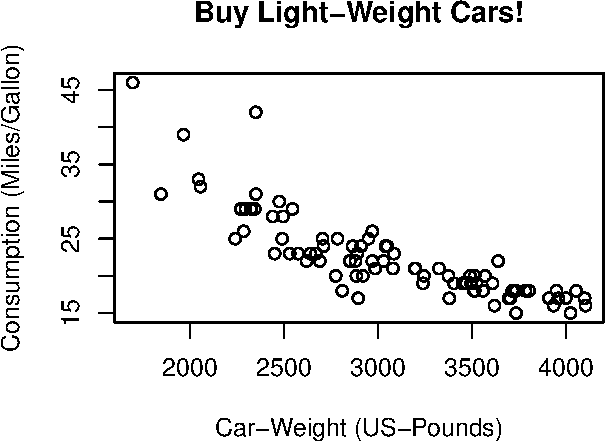
\includegraphics{./01-Introduction-to-R_files/figure-pdf/fig-margin-1.pdf}

}

\caption{\label{fig-margin}\textbf{?(caption)}}

\end{figure}

\hfill\break

As a first step, we might assume a simple kind of linear relationship
between the variables \texttt{gasolin.consumption} and
\texttt{car.weight}. Let us assume that the data was generated by the
following simple regression model:

\[
y_i=\alpha+\beta_1 x_i+\varepsilon_i,\quad i=1,\dots,n
\]

where \(y_i\) denotes the gasoline-consumption, \(x_i\) the weight of
car \(i\), and \(\varepsilon_i\) is a mean zero constant variance noise
term. (This is clearly a non-sense model!)

The command \texttt{lm()} computes the estimates of this linear
regression model. The command (in fact it's a \emph{method})
\texttt{summary()} computes further quantities of general interest from
the \emph{object} that was returned from the \texttt{lm()} function.

\begin{Shaded}
\begin{Highlighting}[]
\NormalTok{lm.result   }\OtherTok{\textless{}{-}} \FunctionTok{lm}\NormalTok{(gasolin.consumption}\SpecialCharTok{\textasciitilde{}}\NormalTok{car.weight)}
\NormalTok{lm.summary  }\OtherTok{\textless{}{-}} \FunctionTok{summary}\NormalTok{(lm.result)}
\NormalTok{lm.summary}
\end{Highlighting}
\end{Shaded}

\begin{verbatim}

Call:
lm(formula = gasolin.consumption ~ car.weight)

Residuals:
    Min      1Q  Median      3Q     Max 
-6.7946 -1.9711  0.0249  1.1855 13.8278 

Coefficients:
             Estimate Std. Error t value Pr(>|t|)    
(Intercept) 47.048353   1.679912   28.01   <2e-16 ***
car.weight  -0.008032   0.000537  -14.96   <2e-16 ***
---
Signif. codes:  0 '***' 0.001 '**' 0.01 '*' 0.05 '.' 0.1 ' ' 1

Residual standard error: 3.038 on 91 degrees of freedom
Multiple R-squared:  0.7109,    Adjusted R-squared:  0.7077 
F-statistic: 223.8 on 1 and 91 DF,  p-value: < 2.2e-16
\end{verbatim}

\hfill\break

Of course, we want to have a possibility to access all the quantities
computed so far, e.g., in order to plot the results. This can be done as
following:

\begin{Shaded}
\begin{Highlighting}[]
\DocumentationTok{\#\# Accessing the computed quantities}
\FunctionTok{names}\NormalTok{(lm.summary) }\DocumentationTok{\#\# Alternatively: str(lm.summary)}
\end{Highlighting}
\end{Shaded}

\begin{verbatim}
 [1] "call"          "terms"         "residuals"     "coefficients" 
 [5] "aliased"       "sigma"         "df"            "r.squared"    
 [9] "adj.r.squared" "fstatistic"    "cov.unscaled" 
\end{verbatim}

\begin{Shaded}
\begin{Highlighting}[]
\NormalTok{alpha }\OtherTok{\textless{}{-}}\NormalTok{ lm.summary}\SpecialCharTok{$}\NormalTok{coefficients[}\DecValTok{1}\NormalTok{]}
\NormalTok{beta  }\OtherTok{\textless{}{-}}\NormalTok{ lm.summary}\SpecialCharTok{$}\NormalTok{coefficients[}\DecValTok{2}\NormalTok{]}

\DocumentationTok{\#\# Plot all:}
\FunctionTok{plot}\NormalTok{(}\AttributeTok{y=}\NormalTok{gasolin.consumption, }\AttributeTok{x=}\NormalTok{car.weight, }
     \AttributeTok{xlab=}\StringTok{"Car{-}Weight (US{-}Pounds)"}\NormalTok{, }
     \AttributeTok{ylab=}\StringTok{"Consumption (Miles/Gallon)"}\NormalTok{, }
     \AttributeTok{main=}\StringTok{"Buy light{-}weight Cars!"}\NormalTok{)}
\FunctionTok{abline}\NormalTok{(}\AttributeTok{a=}\NormalTok{alpha, }
       \AttributeTok{b=}\NormalTok{beta, }\AttributeTok{col=}\StringTok{"red"}\NormalTok{)}
\end{Highlighting}
\end{Shaded}

\begin{figure}[H]

{\centering 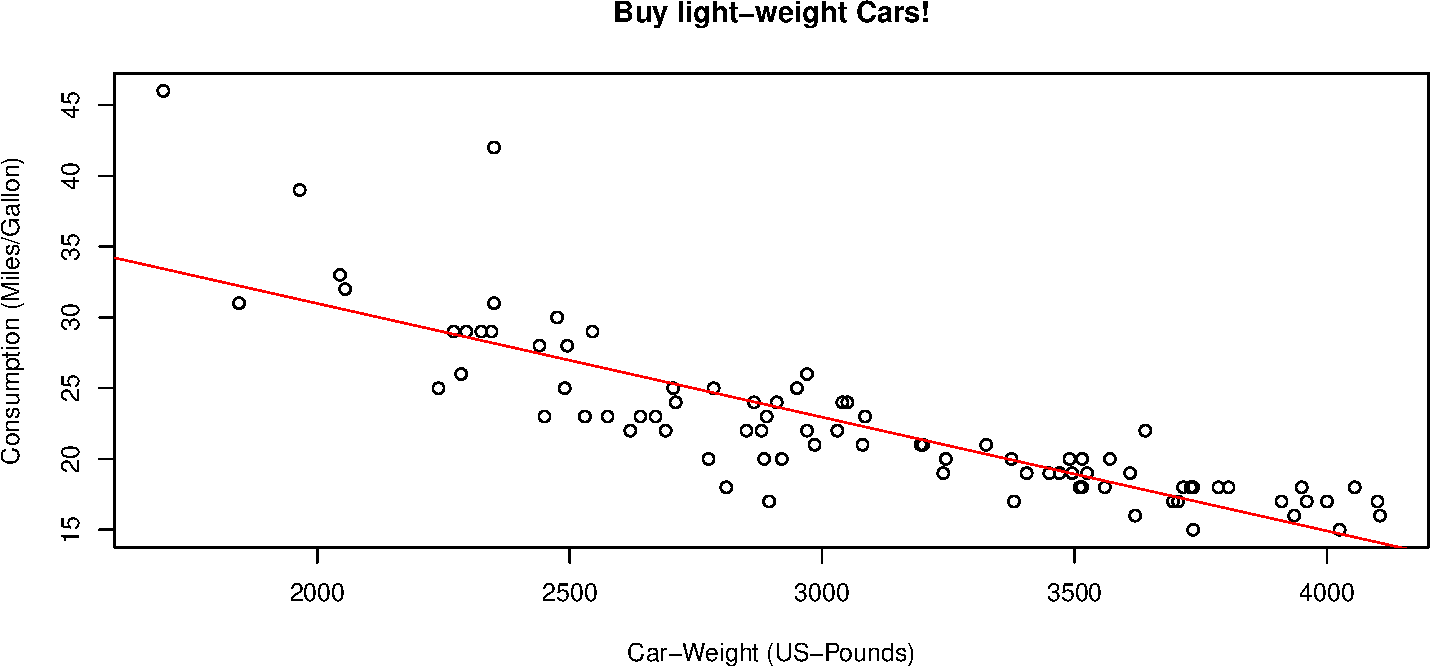
\includegraphics{./01-Introduction-to-R_files/figure-pdf/unnamed-chunk-23-1.pdf}

}

\end{figure}

\hfill\break

\hypertarget{programming-in-r}{%
\section{Programming in R}\label{programming-in-r}}

Let's write, i.e., program our own R-function for estimating linear
regression models. In order to be able to validate our function, we
start with \textbf{simulating data} for which we then \emph{know} all
true parameters. Simulating data is like being the ``Data-God'': For
instance, we generate realizations of the error term \(\varepsilon_i\),
i.e., something which we \emph{never} observe in real data.

\hfill\break

Let us consider the following multiple regression model:

\[y_i=\beta_1 +\beta_2 x_{2i}+\beta_3 x_{3i}+\varepsilon_{i},\quad i=1,\dots,n,\]

where \(\varepsilon_{i}\) is a heteroscedastic error term

\[\varepsilon_{i}\sim N(0,\sigma_i^2),\quad \sigma_i=|x_{3i}|,\]

and where for all \(i=1,\dots,n=50\):

\begin{itemize}
\tightlist
\item
  \(x_{2i}\sim N(10,1.5^2)\)
\item
  \(x_{3i}\) comes from a t-distribution with 5 degrees of freedom and
  non-centrality parameter 2
\end{itemize}

\begin{Shaded}
\begin{Highlighting}[]
\FunctionTok{set.seed}\NormalTok{(}\DecValTok{109}\NormalTok{) }\CommentTok{\# Sets the "seed" of the random number generators:}
\NormalTok{n   }\OtherTok{\textless{}{-}} \DecValTok{50}     \CommentTok{\# Number of observations}

\DocumentationTok{\#\# Generate two explanatory variables plus an intercept{-}variable:}
\NormalTok{X}\FloatTok{.1} \OtherTok{\textless{}{-}} \FunctionTok{rep}\NormalTok{(}\DecValTok{1}\NormalTok{, n)                 }\CommentTok{\# Intercept}
\NormalTok{X}\FloatTok{.2} \OtherTok{\textless{}{-}} \FunctionTok{rnorm}\NormalTok{(n, }\AttributeTok{mean=}\DecValTok{10}\NormalTok{, }\AttributeTok{sd=}\FloatTok{1.5}\NormalTok{) }\CommentTok{\# Draw realizations form a normal distr.}
\NormalTok{X}\FloatTok{.3} \OtherTok{\textless{}{-}} \FunctionTok{rt}\NormalTok{(n, }\AttributeTok{df=}\DecValTok{5}\NormalTok{, }\AttributeTok{ncp=}\DecValTok{2}\NormalTok{)        }\CommentTok{\# Draw realizations form a t{-}distr.}
\NormalTok{X   }\OtherTok{\textless{}{-}} \FunctionTok{cbind}\NormalTok{(X}\FloatTok{.1}\NormalTok{, X}\FloatTok{.2}\NormalTok{, X}\FloatTok{.3}\NormalTok{)      }\CommentTok{\# Save as a Nx3{-}dimensional data matrix.}
\end{Highlighting}
\end{Shaded}

OK, we have regressors, i.e., data that we also have in real data sets.

Now we define the elements of the \(\beta\)-vector. Be aware of the
difference: In real data sets we do not know the true \(\beta\)-vector,
but try to estimate it. However, when simulating data, we determine (as
``Data-Gods'') the true \(\beta\)-vector and can compare our estimate
\(\hat{\beta}\) with the true \(\beta\):

\begin{Shaded}
\begin{Highlighting}[]
\DocumentationTok{\#\# Define the slope{-}coefficients}
\NormalTok{beta.vec  }\OtherTok{\textless{}{-}} \FunctionTok{c}\NormalTok{(}\DecValTok{1}\NormalTok{,}\SpecialCharTok{{-}}\DecValTok{5}\NormalTok{,}\DecValTok{5}\NormalTok{)}
\end{Highlighting}
\end{Shaded}

\hfill\break
We still need to simulate realizations of the dependent variable
\(y_i\). Remember that
\(y_i=\beta_1 x_{1i}+\beta_1 x_{2i}+\beta_3 x_{3i}+\varepsilon_{i}\).
That is, we only need realizations from the error terms
\(\varepsilon_i\) in order to compute the realizations from \(y_i\).
This is how you can simulate realizations from the heteroscedastic error
terms \(\varepsilon_i\):

\begin{Shaded}
\begin{Highlighting}[]
\DocumentationTok{\#\# Generate realizations from the heteroscadastic error term}
\NormalTok{eps       }\OtherTok{\textless{}{-}} \FunctionTok{abs}\NormalTok{(X}\FloatTok{.3}\NormalTok{) }\SpecialCharTok{*} \FunctionTok{rnorm}\NormalTok{(n, }\AttributeTok{mean=}\DecValTok{0}\NormalTok{, }\AttributeTok{sd=}\DecValTok{1}\NormalTok{)}
\end{Highlighting}
\end{Shaded}

Take a look at the heteroscedasticity in the error term:

\begin{Shaded}
\begin{Highlighting}[]
\FunctionTok{plot}\NormalTok{(}\AttributeTok{y=}\NormalTok{eps, }\AttributeTok{x=}\NormalTok{X}\FloatTok{.3}\NormalTok{, }
     \AttributeTok{main=}\StringTok{"Realizations of the }\SpecialCharTok{\textbackslash{}n}\StringTok{Heteroscedastic Error Term"}\NormalTok{)}
\end{Highlighting}
\end{Shaded}

\begin{figure}[H]

{\centering 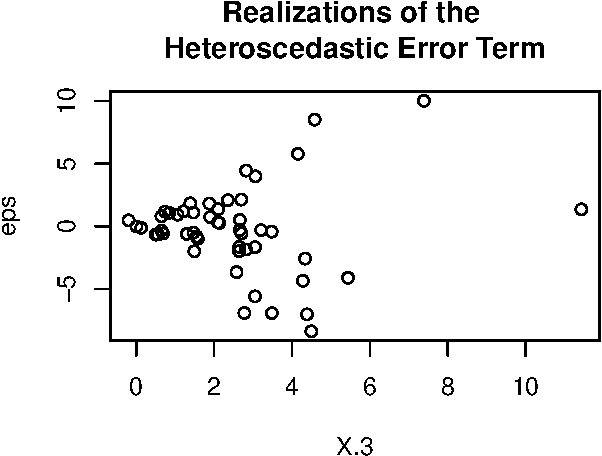
\includegraphics{./01-Introduction-to-R_files/figure-pdf/unnamed-chunk-27-1.pdf}

}

\end{figure}

With the (pseudo-random) realizations from \(\varepsilon_i\), we can
finally generate realizations from the dependent variable \(y_i\):

\begin{Shaded}
\begin{Highlighting}[]
\DocumentationTok{\#\# Dependent variable:}
\NormalTok{y   }\OtherTok{\textless{}{-}}\NormalTok{ X }\SpecialCharTok{\%*\%}\NormalTok{ beta.vec }\SpecialCharTok{+}\NormalTok{ eps}
\end{Highlighting}
\end{Shaded}

Let's take a look at the data:

\begin{Shaded}
\begin{Highlighting}[]
\NormalTok{mydata    }\OtherTok{\textless{}{-}} \FunctionTok{data.frame}\NormalTok{(}\StringTok{"Y"}\OtherTok{=}\NormalTok{y, }\StringTok{"X.1"}\OtherTok{=}\NormalTok{X}\FloatTok{.1}\NormalTok{, }\StringTok{"X.2"}\OtherTok{=}\NormalTok{X}\FloatTok{.2}\NormalTok{, }\StringTok{"X.3"}\OtherTok{=}\NormalTok{X}\FloatTok{.3}\NormalTok{)}
\FunctionTok{pairs}\NormalTok{(mydata[,}\SpecialCharTok{{-}}\DecValTok{2}\NormalTok{]) }\CommentTok{\# The \textquotesingle{}{-}2\textquotesingle{} removes the intercept variable "X.1"}
\end{Highlighting}
\end{Shaded}

\begin{figure}[H]

{\centering 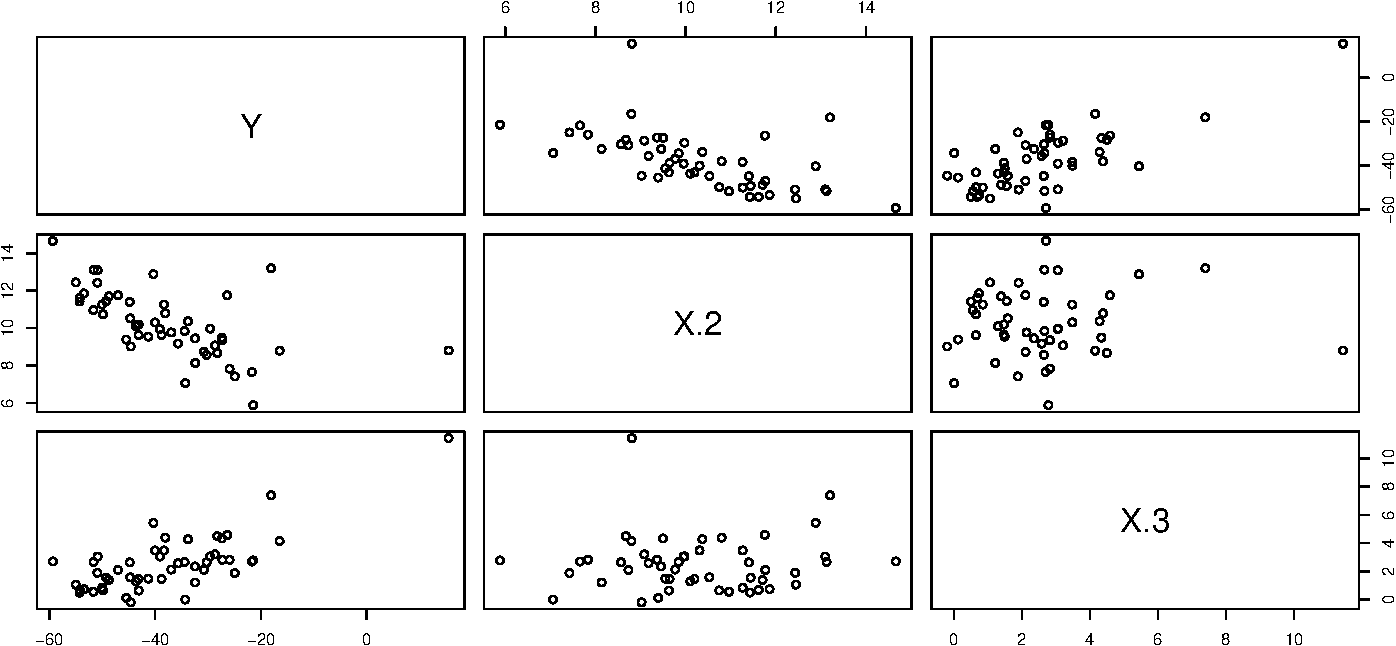
\includegraphics{./01-Introduction-to-R_files/figure-pdf/unnamed-chunk-29-1.pdf}

}

\end{figure}

\hfill\break

Once we have data, we can compute the OLS estimate of the true \(\beta\)
vector. Remember the formula:

\[\hat{\beta}=(X^\top X)^{-1}X^\top y\]

In R-Code this is: \((X^\top X)^{-1}=\)\texttt{solve(t(X)\ \%*\%\ X)},
i.e.:

\begin{Shaded}
\begin{Highlighting}[]
\DocumentationTok{\#\# Computation of the beta{-}Vector:}
\NormalTok{beta.hat }\OtherTok{\textless{}{-}} \FunctionTok{solve}\NormalTok{(}\FunctionTok{t}\NormalTok{(X) }\SpecialCharTok{\%*\%}\NormalTok{ X) }\SpecialCharTok{\%*\%} \FunctionTok{t}\NormalTok{(X) }\SpecialCharTok{\%*\%}\NormalTok{ y}
\NormalTok{beta.hat}
\end{Highlighting}
\end{Shaded}

\begin{verbatim}
         [,1]
X.1 -2.609634
X.2 -4.692735
X.3  5.078342
\end{verbatim}

\hfill\break

Well done. Using the above lines of code we can easily program our own
\texttt{myOLSFun()} function!

\begin{Shaded}
\begin{Highlighting}[]
\NormalTok{myOLSFun }\OtherTok{\textless{}{-}} \ControlFlowTok{function}\NormalTok{(y, x, }\AttributeTok{add.intercept=}\ConstantTok{FALSE}\NormalTok{)\{}
  
  \DocumentationTok{\#\# Number of Observations:}
\NormalTok{  n         }\OtherTok{\textless{}{-}} \FunctionTok{length}\NormalTok{(y)}
  
  \DocumentationTok{\#\# Add an intercept to x:}
  \ControlFlowTok{if}\NormalTok{(add.intercept)\{}
\NormalTok{    Intercept }\OtherTok{\textless{}{-}} \FunctionTok{rep}\NormalTok{(}\DecValTok{1}\NormalTok{, n)}
\NormalTok{    x         }\OtherTok{\textless{}{-}} \FunctionTok{cbind}\NormalTok{(Intercept, x)}
\NormalTok{  \}}
  
  \DocumentationTok{\#\# Estimation of the slope{-}parameters:}
\NormalTok{  beta.hat.vec }\OtherTok{\textless{}{-}} \FunctionTok{solve}\NormalTok{(}\FunctionTok{t}\NormalTok{(x) }\SpecialCharTok{\%*\%}\NormalTok{ x) }\SpecialCharTok{\%*\%} \FunctionTok{t}\NormalTok{(x) }\SpecialCharTok{\%*\%}\NormalTok{ y}
  
  \DocumentationTok{\#\# Return the result:}
  \FunctionTok{return}\NormalTok{(beta.hat.vec)}
\NormalTok{\}}

\DocumentationTok{\#\# Run the function:}
\FunctionTok{myOLSFun}\NormalTok{(}\AttributeTok{y=}\NormalTok{y, }\AttributeTok{x=}\NormalTok{X)}
\end{Highlighting}
\end{Shaded}

\begin{verbatim}
         [,1]
X.1 -2.609634
X.2 -4.692735
X.3  5.078342
\end{verbatim}

\hfill\break

Can you extend the function for the computation of the covariance matrix
of the slope-estimates, several measures of fits (R\(^2\), adj.-R\(^2\),
etc.), t-tests, \ldots?

\hypertarget{r-packages}{%
\section{R-packages}\label{r-packages}}

One of the best features in R are its contributed packages. The list of
all packages on CRAN is impressive! Take a look at it
\href{https://cran.r-project.org/web/packages/available_packages_by_name.html}{HERE}

For instance, nice plots can be produced using the R-package is
\texttt{ggplot2}. You can find an intro do this package
\href{http://ggplot2.tidyverse.org/}{HERE}.

\begin{Shaded}
\begin{Highlighting}[]
\CommentTok{\# install.packages("ggplot2")}
\FunctionTok{library}\NormalTok{(}\StringTok{"ggplot2"}\NormalTok{)}

\FunctionTok{qplot}\NormalTok{(Sepal.Length, Petal.Length, }\AttributeTok{data =}\NormalTok{ iris, }\AttributeTok{color =}\NormalTok{ Species)}
\end{Highlighting}
\end{Shaded}

\begin{figure}[H]

{\centering 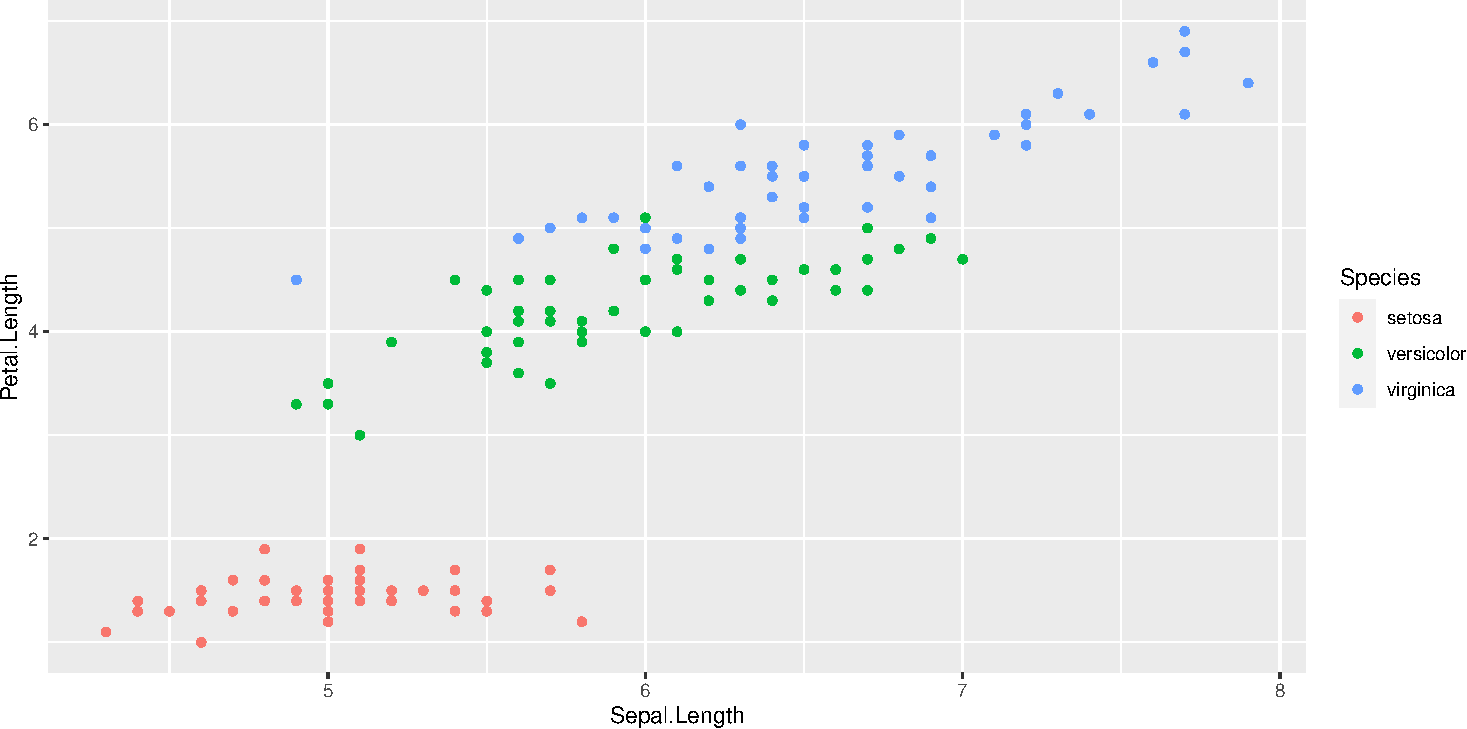
\includegraphics{./01-Introduction-to-R_files/figure-pdf/unnamed-chunk-32-1.pdf}

}

\end{figure}

\hfill\break

Of course, \texttt{ggplot2} concerns ``only'' plotting, but you'll find
R-packages for almost any statistical method out there.

\hypertarget{tidyverse}{%
\section{Tidyverse}\label{tidyverse}}

The \texttt{tidyverse} package is a collection of packages that lets you
import, manipulate, explore, visualize and model data in a harmonized
and consistent way which helps you to be more productive.

Installing the \texttt{tidyverse} package:

\begin{Shaded}
\begin{Highlighting}[]
\FunctionTok{install.packages}\NormalTok{(}\StringTok{"tidyverse"}\NormalTok{)}
\end{Highlighting}
\end{Shaded}

To use the \texttt{tidyverse} package load it using the
\texttt{library()} function:

\begin{Shaded}
\begin{Highlighting}[]
\FunctionTok{library}\NormalTok{(tidyverse)}
\end{Highlighting}
\end{Shaded}

\begin{verbatim}
-- Attaching packages --------------------------------------- tidyverse 1.3.2 --
v tibble  3.1.8      v dplyr   1.0.10
v tidyr   1.2.0      v stringr 1.4.1 
v purrr   0.3.4      v forcats 0.5.2 
-- Conflicts ------------------------------------------ tidyverse_conflicts() --
x dplyr::filter() masks stats::filter()
x dplyr::lag()    masks stats::lag()
\end{verbatim}

\textbf{Chick Weight Data}

R comes with many datasets installed. We will use the
\texttt{ChickWeight} dataset to learn about the tidyverse. The help
system gives a basic summary of the experiment from which the data was
collect:

\begin{quote}
\emph{``The body weights of the chicks were measured at birth and every
second day thereafter until day 20. They were also measured on day 21.
There were four groups of chicks on different protein diets.''}
\end{quote}

You can get more information, including references by typing:

\begin{Shaded}
\begin{Highlighting}[]
\FunctionTok{help}\NormalTok{(}\StringTok{"ChickWeight"}\NormalTok{)}
\end{Highlighting}
\end{Shaded}

\textbf{The Data: } There are 578 observations (rows) and 4 variables:

\begin{itemize}
\tightlist
\item
  \texttt{Chick} -- unique ID for each chick.
\item
  \texttt{Diet} -- one of four protein diets.
\item
  \texttt{Time} -- number of days since birth.
\item
  \texttt{weight} -- body weight of chick in grams.
\end{itemize}

Note: \texttt{weight} has a lower case \texttt{w} (recall R is case
sensitive).

Store the data locally:

\begin{Shaded}
\begin{Highlighting}[]
\NormalTok{ChickWeight }\SpecialCharTok{\%\textgreater{}\%}
  \FunctionTok{select}\NormalTok{(Chick, Diet, Time, weight) }\SpecialCharTok{\%\textgreater{}\%} 
  \FunctionTok{arrange}\NormalTok{(Chick, Diet, Time) }\SpecialCharTok{\%\textgreater{}\%} 
  \FunctionTok{write\_csv}\NormalTok{(}\StringTok{"ChickWeight.csv"}\NormalTok{)}
\end{Highlighting}
\end{Shaded}

First we will import the data from a file called
\texttt{ChickWeight.csv} using the \texttt{read\_csv()} function from
the \texttt{readr} package (part of the \texttt{tidyverse}). The first
thing to do, outside of R, is to open the file \texttt{ChickWeight.csv}
to check what it contains and that it makes sense. Now we can import the
data as follows:

\begin{Shaded}
\begin{Highlighting}[]
\NormalTok{CW }\OtherTok{\textless{}{-}} \FunctionTok{read\_csv}\NormalTok{(}\StringTok{"ChickWeight.csv"}\NormalTok{)}
\end{Highlighting}
\end{Shaded}

\begin{verbatim}
Rows: 578 Columns: 4
-- Column specification --------------------------------------------------------
Delimiter: ","
dbl (4): Chick, Diet, Time, weight

i Use `spec()` to retrieve the full column specification for this data.
i Specify the column types or set `show_col_types = FALSE` to quiet this message.
\end{verbatim}

If all goes well then the data is now stored in an R object called
\texttt{CW}. If you get the following error message then you need to
change the working directory to where the data is stored.

\begin{verbatim}
Error: 'ChickWeight.csv' does not exist in current
working directory ...
\end{verbatim}

\textbf{Changing the working directory:} In RStudio you can use the menu
bar (``Session - Set Working Directory - Choose Directory\ldots{}'').
Alternatively, you can use the function \texttt{setwd()}.

\hfill\break

\textbf{Looking at the Dataset:} To look at the data type just type the
object (dataset) name:

\begin{Shaded}
\begin{Highlighting}[]
\NormalTok{CW}
\end{Highlighting}
\end{Shaded}

\begin{verbatim}
# A tibble: 578 x 4
   Chick  Diet  Time weight
   <dbl> <dbl> <dbl>  <dbl>
 1    18     1     0     39
 2    18     1     2     35
 3    16     1     0     41
 4    16     1     2     45
 5    16     1     4     49
 6    16     1     6     51
 7    16     1     8     57
 8    16     1    10     51
 9    16     1    12     54
10    15     1     0     41
# ... with 568 more rows
\end{verbatim}

If there are too many variables then not all them may be printed. To
overcome this issue we can use the \texttt{glimpse()} function which
makes it possible to see every column in your dataset (called a ``data
frame'' in R speak).

\begin{Shaded}
\begin{Highlighting}[]
\FunctionTok{glimpse}\NormalTok{(CW)}
\end{Highlighting}
\end{Shaded}

\begin{verbatim}
Rows: 578
Columns: 4
$ Chick  <dbl> 18, 18, 16, 16, 16, 16, 16, 16, 16, 15, 15, 15, 15, 15, 15, 15,~
$ Diet   <dbl> 1, 1, 1, 1, 1, 1, 1, 1, 1, 1, 1, 1, 1, 1, 1, 1, 1, 1, 1, 1, 1, ~
$ Time   <dbl> 0, 2, 0, 2, 4, 6, 8, 10, 12, 0, 2, 4, 6, 8, 10, 12, 14, 0, 2, 4~
$ weight <dbl> 39, 35, 41, 45, 49, 51, 57, 51, 54, 41, 49, 56, 64, 68, 68, 67,~
\end{verbatim}

The function \texttt{View()} allows for a spread-sheet type of view on
the data:

\begin{Shaded}
\begin{Highlighting}[]
\FunctionTok{View}\NormalTok{(CW)}
\end{Highlighting}
\end{Shaded}

\hypertarget{tidyverse-plotting-basics}{%
\subsection{Tidyverse: Plotting
Basics}\label{tidyverse-plotting-basics}}

To \textbf{visualise} the chick weight data, we will use the
\texttt{ggplot2} package (part of the \texttt{tidyverse}). Our interest
is in seeing how the \emph{weight changes over time for the chicks by
diet}. For the moment don't worry too much about the details just try to
build your own understanding and logic. To learn more try different
things even if you get an error messages.

Let's plot the weight data (vertical axis) over time (horizontal axis).

\begin{Shaded}
\begin{Highlighting}[]
\CommentTok{\# An empty plot (the plot on the left)}
\FunctionTok{ggplot}\NormalTok{(CW, }\FunctionTok{aes}\NormalTok{(Time, weight))  }
\CommentTok{\# With data (the plot on the right)}
\FunctionTok{ggplot}\NormalTok{(CW, }\FunctionTok{aes}\NormalTok{(Time, weight)) }\SpecialCharTok{+} \FunctionTok{geom\_point}\NormalTok{() }
\end{Highlighting}
\end{Shaded}

\begin{figure}[H]

{\centering 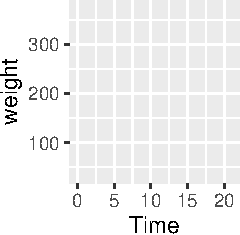
\includegraphics{./01-Introduction-to-R_files/figure-pdf/emptyPlot-1.pdf}

}

\end{figure}

\begin{figure}[H]

{\centering 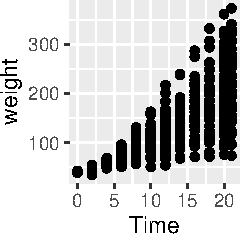
\includegraphics{./01-Introduction-to-R_files/figure-pdf/emptyPlot-2.pdf}

}

\end{figure}

Add color for \texttt{Diet}. The graph above does not differentiate
between the diets. Let's use a different color for each diet.

\begin{Shaded}
\begin{Highlighting}[]
\CommentTok{\# Adding colour for diet}
\FunctionTok{ggplot}\NormalTok{(CW,}\FunctionTok{aes}\NormalTok{(Time,weight,}\AttributeTok{colour=}\FunctionTok{factor}\NormalTok{(Diet))) }\SpecialCharTok{+}
  \FunctionTok{geom\_point}\NormalTok{() }
\end{Highlighting}
\end{Shaded}

\begin{figure}[H]

{\centering 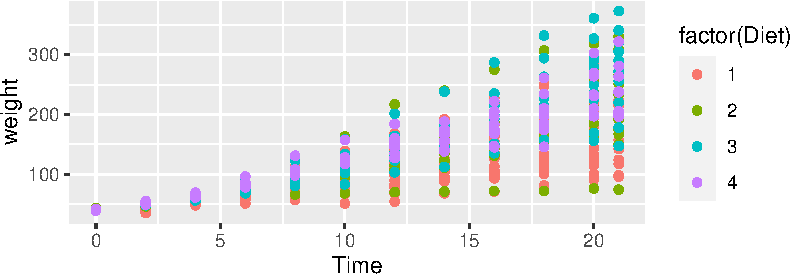
\includegraphics{./01-Introduction-to-R_files/figure-pdf/addColourPlot-1.pdf}

}

\end{figure}

It is difficult to conclude anything from this graph as the points are
printed on top of one another (with diet 1 underneath and diet 4 at the
top).

\textbf{Factor Variables:} Before we continue, we have to make an
important change to the \texttt{CW} dataset by making \texttt{Diet} and
\texttt{Time} \emph{factor variables}. This means that R will treat them
as categorical variables (see the \texttt{\textless{}fct\textgreater{}}
variables below) instead of continuous variables. It will simplify our
coding. The next section will explain the \texttt{mutate()} function.

\begin{Shaded}
\begin{Highlighting}[]
\NormalTok{CW }\OtherTok{\textless{}{-}} \FunctionTok{mutate}\NormalTok{(CW, }\AttributeTok{Diet =} \FunctionTok{factor}\NormalTok{(Diet))}
\NormalTok{CW }\OtherTok{\textless{}{-}} \FunctionTok{mutate}\NormalTok{(CW, }\AttributeTok{Time =} \FunctionTok{factor}\NormalTok{(Time))}
\FunctionTok{glimpse}\NormalTok{(CW)}
\end{Highlighting}
\end{Shaded}

\begin{verbatim}
Rows: 578
Columns: 4
$ Chick  <dbl> 18, 18, 16, 16, 16, 16, 16, 16, 16, 15, 15, 15, 15, 15, 15, 15,~
$ Diet   <fct> 1, 1, 1, 1, 1, 1, 1, 1, 1, 1, 1, 1, 1, 1, 1, 1, 1, 1, 1, 1, 1, ~
$ Time   <fct> 0, 2, 0, 2, 4, 6, 8, 10, 12, 0, 2, 4, 6, 8, 10, 12, 14, 0, 2, 4~
$ weight <dbl> 39, 35, 41, 45, 49, 51, 57, 51, 54, 41, 49, 56, 64, 68, 68, 67,~
\end{verbatim}

The \texttt{facet\_wrap()} function: To plot each diet separately in a
grid using \texttt{facet\_wrap()}:

\begin{Shaded}
\begin{Highlighting}[]
\CommentTok{\# Adding jitter to the points}
\FunctionTok{ggplot}\NormalTok{(CW, }\FunctionTok{aes}\NormalTok{(Time, weight, }\AttributeTok{colour=}\NormalTok{Diet)) }\SpecialCharTok{+}
  \FunctionTok{geom\_point}\NormalTok{() }\SpecialCharTok{+}
  \FunctionTok{facet\_wrap}\NormalTok{(}\SpecialCharTok{\textasciitilde{}}\NormalTok{Diet) }\SpecialCharTok{+}
  \FunctionTok{theme}\NormalTok{(}\AttributeTok{legend.position =} \StringTok{"bottom"}\NormalTok{)}
\end{Highlighting}
\end{Shaded}

\begin{figure}[H]

{\centering 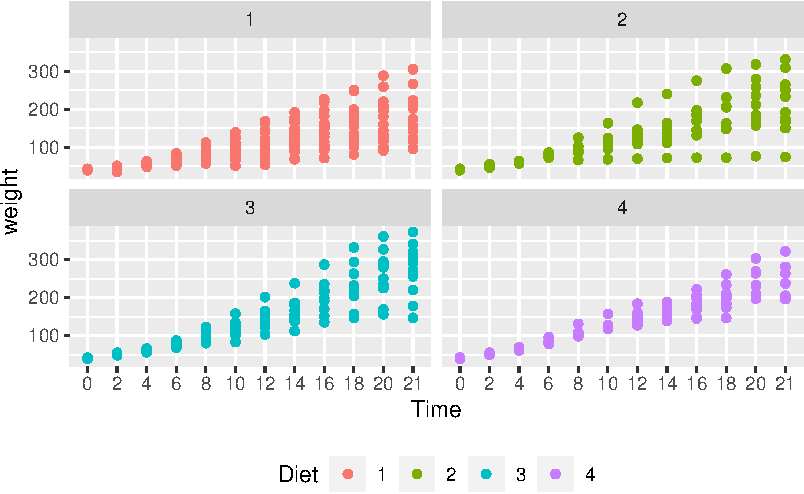
\includegraphics{./01-Introduction-to-R_files/figure-pdf/ScatterPlot-1.pdf}

}

\end{figure}

\textbf{Interpretation:} Diet 4 has the least variability but we can't
really say anything about the mean effect of each diet although diet 3
seems to have the highest.

Next we will plot the \textbf{mean changes} over time for each diet
using the \texttt{stat\_summary()} function:

\begin{Shaded}
\begin{Highlighting}[]
\FunctionTok{ggplot}\NormalTok{(CW, }\FunctionTok{aes}\NormalTok{(Time, weight, }
               \AttributeTok{group=}\NormalTok{Diet, }\AttributeTok{colour=}\NormalTok{Diet)) }\SpecialCharTok{+}
  \FunctionTok{stat\_summary}\NormalTok{(}\AttributeTok{fun=}\StringTok{"mean"}\NormalTok{, }\AttributeTok{geom=}\StringTok{"line"}\NormalTok{) }
\end{Highlighting}
\end{Shaded}

\begin{figure}[H]

{\centering 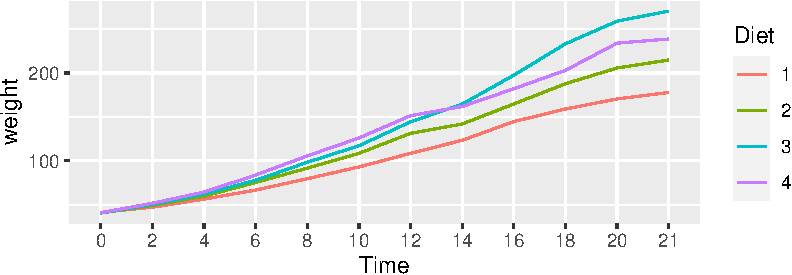
\includegraphics{./01-Introduction-to-R_files/figure-pdf/meanlinesPlot-1.pdf}

}

\end{figure}

\textbf{Interpretation:} We can see that diet 3 has the highest mean
weight gains by the end of the experiment. However, we don't have any
information about the variation (uncertainty) in the data.

To see variation between the different diets we use
\texttt{geom\_boxplot} to plot a box-whisker plot. A note of caution is
that the number of chicks per diet is relatively low to produce this
plot.

\begin{Shaded}
\begin{Highlighting}[]
\FunctionTok{ggplot}\NormalTok{(CW, }\FunctionTok{aes}\NormalTok{(Time, weight, }\AttributeTok{colour=}\NormalTok{Diet)) }\SpecialCharTok{+}
  \FunctionTok{facet\_wrap}\NormalTok{(}\SpecialCharTok{\textasciitilde{}}\NormalTok{Diet) }\SpecialCharTok{+}
  \FunctionTok{geom\_boxplot}\NormalTok{() }\SpecialCharTok{+}
  \FunctionTok{theme}\NormalTok{(}\AttributeTok{legend.position =} \StringTok{"none"}\NormalTok{) }\SpecialCharTok{+}
  \FunctionTok{ggtitle}\NormalTok{(}\StringTok{"Chick Weight over Time by Diet"}\NormalTok{)}
\end{Highlighting}
\end{Shaded}

\begin{figure}[H]

{\centering 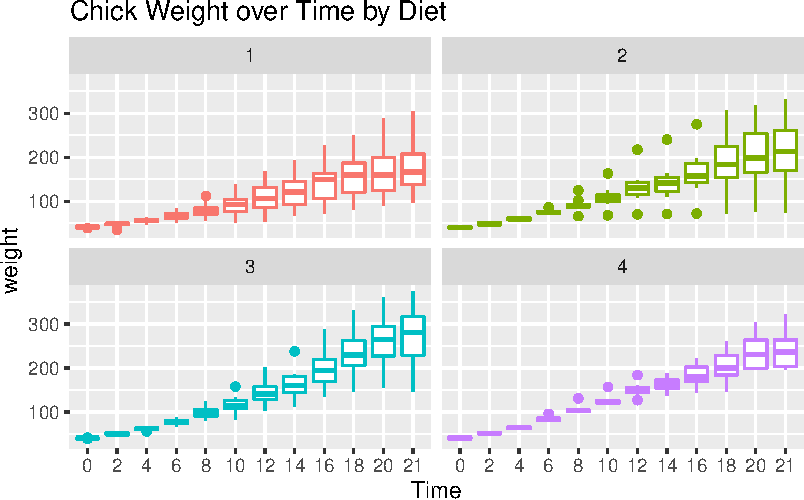
\includegraphics{./01-Introduction-to-R_files/figure-pdf/boxPlot-1.pdf}

}

\end{figure}

\textbf{Interpretation:} Diet 3 seems to have the highest ``average''
weight gain but it has more variation than diet 4 which is consistent
with our findings so far.

Let's finish with a plot that you might include in a publication.

\begin{Shaded}
\begin{Highlighting}[]
\FunctionTok{ggplot}\NormalTok{(CW, }\FunctionTok{aes}\NormalTok{(Time, weight, }\AttributeTok{group=}\NormalTok{Diet, }
                             \AttributeTok{colour=}\NormalTok{Diet)) }\SpecialCharTok{+}
  \FunctionTok{facet\_wrap}\NormalTok{(}\SpecialCharTok{\textasciitilde{}}\NormalTok{Diet) }\SpecialCharTok{+}
  \FunctionTok{geom\_point}\NormalTok{() }\SpecialCharTok{+}
  \CommentTok{\# geom\_jitter() +}
  \FunctionTok{stat\_summary}\NormalTok{(}\AttributeTok{fun=}\StringTok{"mean"}\NormalTok{, }\AttributeTok{geom=}\StringTok{"line"}\NormalTok{,}
               \AttributeTok{colour=}\StringTok{"black"}\NormalTok{) }\SpecialCharTok{+}
  \FunctionTok{theme}\NormalTok{(}\AttributeTok{legend.position =} \StringTok{"none"}\NormalTok{) }\SpecialCharTok{+}
  \FunctionTok{ggtitle}\NormalTok{(}\StringTok{"Chick Weight over Time by Diet"}\NormalTok{) }\SpecialCharTok{+} 
  \FunctionTok{xlab}\NormalTok{(}\StringTok{"Time (days)"}\NormalTok{) }\SpecialCharTok{+}
  \FunctionTok{ylab}\NormalTok{(}\StringTok{"Weight (grams)"}\NormalTok{)}
\end{Highlighting}
\end{Shaded}

\begin{figure}[H]

{\centering 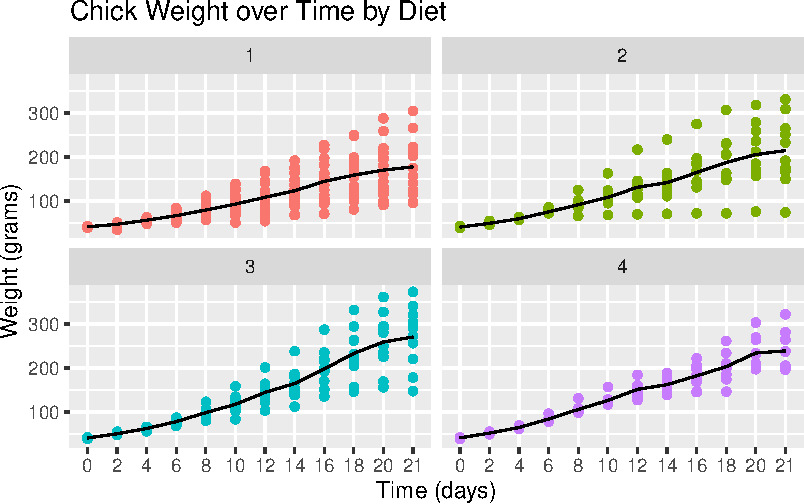
\includegraphics{./01-Introduction-to-R_files/figure-pdf/finalPlot-1.pdf}

}

\end{figure}

\hypertarget{tidyverse-data-wrangling-basics}{%
\subsection{Tidyverse: Data Wrangling
Basics}\label{tidyverse-data-wrangling-basics}}

In this section we will learn how to wrangle (manipulate) datasets using
the \texttt{tidyverse} package. Let's start with the \texttt{mutate()},
\texttt{select()}, \texttt{rename()}, \texttt{filter()} and
\texttt{arrange()} functions.

\hfill\break

\texttt{mutate()}: Adds a new variable (column) or modifies an existing
one. We already used this above to create factor variables.

\begin{Shaded}
\begin{Highlighting}[]
\CommentTok{\# Added a column}
\NormalTok{CWm1 }\OtherTok{\textless{}{-}} \FunctionTok{mutate}\NormalTok{(CW, }\AttributeTok{weightKg =}\NormalTok{ weight}\SpecialCharTok{/}\DecValTok{1000}\NormalTok{)}
\NormalTok{CWm1}
\end{Highlighting}
\end{Shaded}

\begin{verbatim}
# A tibble: 578 x 5
  Chick Diet  Time  weight weightKg
  <dbl> <fct> <fct>  <dbl>    <dbl>
1    18 1     0         39    0.039
2    18 1     2         35    0.035
3    16 1     0         41    0.041
# ... with 575 more rows
\end{verbatim}

\begin{Shaded}
\begin{Highlighting}[]
\CommentTok{\# Modify an existing column}
\NormalTok{CWm2 }\OtherTok{\textless{}{-}} \FunctionTok{mutate}\NormalTok{(CW, }\AttributeTok{Diet =} \FunctionTok{str\_c}\NormalTok{(}\StringTok{"Diet "}\NormalTok{, Diet))}
\NormalTok{CWm2}
\end{Highlighting}
\end{Shaded}

\begin{verbatim}
# A tibble: 578 x 4
  Chick Diet   Time  weight
  <dbl> <chr>  <fct>  <dbl>
1    18 Diet 1 0         39
2    18 Diet 1 2         35
3    16 Diet 1 0         41
# ... with 575 more rows
\end{verbatim}

\hfill\break

\texttt{select()}: Keeps, drops or reorders variables.

\begin{Shaded}
\begin{Highlighting}[]
\CommentTok{\# Drop the weight variable from CWm1 using minus}
\FunctionTok{select}\NormalTok{(CWm1, }\SpecialCharTok{{-}}\NormalTok{weight)}
\end{Highlighting}
\end{Shaded}

\begin{verbatim}
# A tibble: 578 x 4
  Chick Diet  Time  weightKg
  <dbl> <fct> <fct>    <dbl>
1    18 1     0        0.039
2    18 1     2        0.035
3    16 1     0        0.041
# ... with 575 more rows
\end{verbatim}

\begin{Shaded}
\begin{Highlighting}[]
\CommentTok{\# Keep variables Time, Diet and weightKg}
\FunctionTok{select}\NormalTok{(CWm1, Chick, Time, Diet, weightKg)}
\end{Highlighting}
\end{Shaded}

\begin{verbatim}
# A tibble: 578 x 4
  Chick Time  Diet  weightKg
  <dbl> <fct> <fct>    <dbl>
1    18 0     1        0.039
2    18 2     1        0.035
3    16 0     1        0.041
# ... with 575 more rows
\end{verbatim}

\hfill\break

\texttt{rename()}: Renames variables whilst keeping all variables.

\begin{Shaded}
\begin{Highlighting}[]
\FunctionTok{rename}\NormalTok{(CW, }\AttributeTok{Group =}\NormalTok{ Diet, }\AttributeTok{Weight =}\NormalTok{ weight)}
\end{Highlighting}
\end{Shaded}

\begin{verbatim}
# A tibble: 578 x 4
  Chick Group Time  Weight
  <dbl> <fct> <fct>  <dbl>
1    18 1     0         39
2    18 1     2         35
3    16 1     0         41
# ... with 575 more rows
\end{verbatim}

\hfill\break

\texttt{filter()}: Keeps or drops observations (rows).

\begin{Shaded}
\begin{Highlighting}[]
\FunctionTok{filter}\NormalTok{(CW, Time}\SpecialCharTok{==}\DecValTok{21} \SpecialCharTok{\&}\NormalTok{ weight}\SpecialCharTok{\textgreater{}}\DecValTok{300}\NormalTok{)}
\end{Highlighting}
\end{Shaded}

\begin{verbatim}
# A tibble: 8 x 4
  Chick Diet  Time  weight
  <dbl> <fct> <fct>  <dbl>
1     7 1     21       305
2    29 2     21       309
3    21 2     21       331
# ... with 5 more rows
\end{verbatim}

For comparing values in vectors use: \texttt{\textless{}} (less than),
\texttt{\textgreater{}} (greater than), \texttt{\textless{}=} (less than
and equal to), \texttt{\textgreater{}=} (greater than and equal to),
\texttt{==} (equal to) and \texttt{!=} (not equal to). These can be
combined logically using \texttt{\&} (and) and \texttt{\textbar{}} (or).

\hfill\break

\texttt{arrange()}: Changes the order of the observations.

\begin{Shaded}
\begin{Highlighting}[]
\FunctionTok{arrange}\NormalTok{(CW, Chick, Time)}
\end{Highlighting}
\end{Shaded}

\begin{verbatim}
# A tibble: 578 x 4
  Chick Diet  Time  weight
  <dbl> <fct> <fct>  <dbl>
1     1 1     0         42
2     1 1     2         51
3     1 1     4         59
# ... with 575 more rows
\end{verbatim}

\begin{Shaded}
\begin{Highlighting}[]
\FunctionTok{arrange}\NormalTok{(CW, }\FunctionTok{desc}\NormalTok{(weight))}
\end{Highlighting}
\end{Shaded}

\begin{verbatim}
# A tibble: 578 x 4
  Chick Diet  Time  weight
  <dbl> <fct> <fct>  <dbl>
1    35 3     21       373
2    35 3     20       361
3    34 3     21       341
# ... with 575 more rows
\end{verbatim}

What does the \texttt{desc()} do? Try using \texttt{desc(Time)}.

\hypertarget{the-pipe-operator}{%
\subsection{\texorpdfstring{The pipe operator
\texttt{\%\textgreater{}\%}}{The pipe operator \%\textgreater\%}}\label{the-pipe-operator}}

In reality you will end up doing multiple data wrangling steps that you
want to save. The pipe operator \texttt{\%\textgreater{}\%} makes your
code nice and readable:

\begin{Shaded}
\begin{Highlighting}[]
\NormalTok{CW21 }\OtherTok{\textless{}{-}}\NormalTok{ CW }\SpecialCharTok{\%\textgreater{}\%} 
  \FunctionTok{filter}\NormalTok{(Time }\SpecialCharTok{\%in\%} \FunctionTok{c}\NormalTok{(}\DecValTok{0}\NormalTok{, }\DecValTok{21}\NormalTok{)) }\SpecialCharTok{\%\textgreater{}\%} 
  \FunctionTok{rename}\NormalTok{(}\AttributeTok{Weight =}\NormalTok{ weight) }\SpecialCharTok{\%\textgreater{}\%} 
  \FunctionTok{mutate}\NormalTok{(}\AttributeTok{Group =} \FunctionTok{factor}\NormalTok{(}\FunctionTok{str\_c}\NormalTok{(}\StringTok{"Diet "}\NormalTok{, Diet))) }\SpecialCharTok{\%\textgreater{}\%} 
  \FunctionTok{select}\NormalTok{(Chick, Group, Time, Weight) }\SpecialCharTok{\%\textgreater{}\%} 
  \FunctionTok{arrange}\NormalTok{(Chick, Time) }
\NormalTok{CW21}
\end{Highlighting}
\end{Shaded}

\begin{verbatim}
# A tibble: 95 x 4
  Chick Group  Time  Weight
  <dbl> <fct>  <fct>  <dbl>
1     1 Diet 1 0         42
2     1 Diet 1 21       205
3     2 Diet 1 0         40
# ... with 92 more rows
\end{verbatim}

Hint: To understand the code above we should read the pipe operator
\texttt{\%\textgreater{}\%} as ``then''.

\begin{quote}
Create a new dataset (object) called \texttt{CW21} using dataset
\texttt{CW} \textbf{\emph{then}} keep the data for days 0 and 21
\textbf{\emph{then}} rename variable \texttt{weight} to \texttt{Weight}
\textbf{\emph{then}} create a variable called \texttt{Group}
\textbf{\emph{then}} keep variables \texttt{Chick}, \texttt{Group},
\texttt{Time} and \texttt{Weight} and \textbf{\emph{then}} finally
arrange the data by variables \texttt{Chick} and \texttt{Time}.
\end{quote}

This is the same code:

\begin{Shaded}
\begin{Highlighting}[]
\NormalTok{CW21 }\OtherTok{\textless{}{-}}\NormalTok{ CW }\SpecialCharTok{\%\textgreater{}\%} 
  \FunctionTok{filter}\NormalTok{(., Time }\SpecialCharTok{\%in\%} \FunctionTok{c}\NormalTok{(}\DecValTok{0}\NormalTok{, }\DecValTok{21}\NormalTok{)) }\SpecialCharTok{\%\textgreater{}\%} 
  \FunctionTok{rename}\NormalTok{(., }\AttributeTok{Weight =}\NormalTok{ weight) }\SpecialCharTok{\%\textgreater{}\%} 
  \FunctionTok{mutate}\NormalTok{(., }\AttributeTok{Group=}\FunctionTok{factor}\NormalTok{(}\FunctionTok{str\_c}\NormalTok{(}\StringTok{"Diet "}\NormalTok{,Diet))) }\SpecialCharTok{\%\textgreater{}\%} 
  \FunctionTok{select}\NormalTok{(., Chick, Group, Time, Weight) }\SpecialCharTok{\%\textgreater{}\%} 
  \FunctionTok{arrange}\NormalTok{(., Chick, Time) }
\end{Highlighting}
\end{Shaded}

The pipe operator, \texttt{\%\textgreater{}\%}, replaces the dots
(\texttt{.}) with whatever is returned from code preceding it. For
example, the dot in \texttt{filter(.,\ Time\ \%in\%\ c(0,\ 21))} is
replaced by \texttt{CW}. The output of the \texttt{filter(...)} then
replaces the dot in \texttt{rename(.,\ Weight\ =\ weight)} and so on.
Think of it as a data assembly line with each function doing its thing
and passing it to the next.

\hypertarget{the-group_by-function}{%
\subsection{\texorpdfstring{The \texttt{group\_by()}
function}{The group\_by() function}}\label{the-group_by-function}}

From the data visualizations above we concluded that the diet 3 has the
highest mean and diet 4 the least variation. In this section, we will
quantify the effects of the diets using \textbf{summmary statistics}. We
start by looking at the number of observations and the mean by
\textbf{diet} and \textbf{time}.

\begin{Shaded}
\begin{Highlighting}[]
\NormalTok{mnsdCW }\OtherTok{\textless{}{-}}\NormalTok{ CW }\SpecialCharTok{\%\textgreater{}\%} 
  \FunctionTok{group\_by}\NormalTok{(Diet, Time) }\SpecialCharTok{\%\textgreater{}\%} 
  \FunctionTok{summarise}\NormalTok{(}\AttributeTok{N =} \FunctionTok{n}\NormalTok{(), }\AttributeTok{Mean =} \FunctionTok{mean}\NormalTok{(weight)) }\SpecialCharTok{\%\textgreater{}\%} 
  \FunctionTok{arrange}\NormalTok{(Diet, Time)}
\end{Highlighting}
\end{Shaded}

\begin{verbatim}
`summarise()` has grouped output by 'Diet'. You can override using the
`.groups` argument.
\end{verbatim}

\begin{Shaded}
\begin{Highlighting}[]
\NormalTok{mnsdCW}
\end{Highlighting}
\end{Shaded}

\begin{verbatim}
# A tibble: 48 x 4
# Groups:   Diet [4]
  Diet  Time      N  Mean
  <fct> <fct> <int> <dbl>
1 1     0        20  41.4
2 1     2        20  47.2
3 1     4        19  56.5
# ... with 45 more rows
\end{verbatim}

For each distinct combination of \texttt{Diet} and \texttt{Time}, the
chick weight data is summarized into the number of observations
(\texttt{N}) and the mean (\texttt{Mean}) of \texttt{weight}.

\textbf{Further summaries:} Let's also calculate the standard deviation,
median, minimum and maximum values but only at days 0 and 21.

\begin{Shaded}
\begin{Highlighting}[]
\NormalTok{sumCW }\OtherTok{\textless{}{-}}\NormalTok{  CW }\SpecialCharTok{\%\textgreater{}\%} 
  \FunctionTok{filter}\NormalTok{(Time }\SpecialCharTok{\%in\%} \FunctionTok{c}\NormalTok{(}\DecValTok{0}\NormalTok{, }\DecValTok{21}\NormalTok{)) }\SpecialCharTok{\%\textgreater{}\%} 
  \FunctionTok{group\_by}\NormalTok{(Diet, Time) }\SpecialCharTok{\%\textgreater{}\%} 
  \FunctionTok{summarise}\NormalTok{(}\AttributeTok{N =} \FunctionTok{n}\NormalTok{(),}
            \AttributeTok{Mean =} \FunctionTok{mean}\NormalTok{(weight),}
            \AttributeTok{SD =} \FunctionTok{sd}\NormalTok{(weight),}
            \AttributeTok{Median =} \FunctionTok{median}\NormalTok{(weight),}
            \AttributeTok{Min =} \FunctionTok{min}\NormalTok{(weight),}
            \AttributeTok{Max =} \FunctionTok{max}\NormalTok{(weight)) }\SpecialCharTok{\%\textgreater{}\%} 
  \FunctionTok{arrange}\NormalTok{(Diet, Time)}
\end{Highlighting}
\end{Shaded}

\begin{verbatim}
`summarise()` has grouped output by 'Diet'. You can override using the
`.groups` argument.
\end{verbatim}

\begin{Shaded}
\begin{Highlighting}[]
\NormalTok{sumCW}
\end{Highlighting}
\end{Shaded}

\begin{verbatim}
# A tibble: 8 x 8
# Groups:   Diet [4]
  Diet  Time      N  Mean     SD Median   Min   Max
  <fct> <fct> <int> <dbl>  <dbl>  <dbl> <dbl> <dbl>
1 1     0        20  41.4  0.995   41      39    43
2 1     21       16 178.  58.7    166      96   305
3 2     0        10  40.7  1.49    40.5    39    43
# ... with 5 more rows
\end{verbatim}

Let's make the summaries ``prettier'', say, for a report or publication.

\begin{Shaded}
\begin{Highlighting}[]
\FunctionTok{library}\NormalTok{(}\StringTok{"knitr"}\NormalTok{) }\CommentTok{\# to use the kable() function}
\NormalTok{prettySumCW }\OtherTok{\textless{}{-}}\NormalTok{ sumCW }\SpecialCharTok{\%\textgreater{}\%} 
 \FunctionTok{mutate}\NormalTok{(}\StringTok{\textasciigrave{}}\AttributeTok{Mean (SD)}\StringTok{\textasciigrave{}} \OtherTok{=} \FunctionTok{str\_c}\NormalTok{(}\FunctionTok{format}\NormalTok{(Mean, }\AttributeTok{digits=}\DecValTok{1}\NormalTok{),}
           \StringTok{" ("}\NormalTok{, }\FunctionTok{format}\NormalTok{(SD, }\AttributeTok{digits=}\DecValTok{2}\NormalTok{), }\StringTok{")"}\NormalTok{)) }\SpecialCharTok{\%\textgreater{}\%} 
 \FunctionTok{mutate}\NormalTok{(}\AttributeTok{Range =} \FunctionTok{str\_c}\NormalTok{(Min, }\StringTok{" {-} "}\NormalTok{, Max)) }\SpecialCharTok{\%\textgreater{}\%} 
 \FunctionTok{select}\NormalTok{(Diet, Time, N, }\StringTok{\textasciigrave{}}\AttributeTok{Mean (SD)}\StringTok{\textasciigrave{}}\NormalTok{, Median, Range) }\SpecialCharTok{\%\textgreater{}\%}
 \FunctionTok{arrange}\NormalTok{(Diet, Time) }\SpecialCharTok{\%\textgreater{}\%} 
 \FunctionTok{kable}\NormalTok{(}\AttributeTok{format =} \StringTok{"latex"}\NormalTok{)}
\NormalTok{prettySumCW}
\end{Highlighting}
\end{Shaded}

\begin{tabular}{l|l|r|l|r|l}
\hline
Diet & Time & N & Mean (SD) & Median & Range\\
\hline
1 & 0 & 20 & 41 ( 0.99) & 41.0 & 39 - 43\\
\hline
1 & 21 & 16 & 178 (58.70) & 166.0 & 96 - 305\\
\hline
2 & 0 & 10 & 41 ( 1.5) & 40.5 & 39 - 43\\
\hline
2 & 21 & 10 & 215 (78.1) & 212.5 & 74 - 331\\
\hline
3 & 0 & 10 & 41 ( 1) & 41.0 & 39 - 42\\
\hline
3 & 21 & 10 & 270 (72) & 281.0 & 147 - 373\\
\hline
4 & 0 & 10 & 41 ( 1.1) & 41.0 & 39 - 42\\
\hline
4 & 21 & 9 & 239 (43.3) & 237.0 & 196 - 322\\
\hline
\end{tabular}

\textbf{Interpretation:} This summary table offers the same
interpretation as before, namely that diet 3 has the highest mean and
median weights at day 21 but a higher variation than group 4. However it
should be noted that at day 21, diet 1 lost 4 chicks from 20 that
started and diet 4 lost 1 from 10. This could be a sign of some health
related issues.

\hypertarget{further-links}{%
\section{Further Links}\label{further-links}}

\hypertarget{further-r-intros}{%
\subsection{Further R-Intros}\label{further-r-intros}}

\begin{itemize}
\item
  https://eddelbuettel.github.io/gsir-te/Getting-Started-in-R.pdf
\item
  https://www.datacamp.com/courses/free-introduction-to-r
\item
  https://swcarpentry.github.io/r-novice-gapminder/
\item
  https://support.rstudio.com/hc/en-us/articles/200526207-Using-Projects
\end{itemize}

\hypertarget{version-control-gitgithub}{%
\subsection{Version Control
(Git/GitHub)}\label{version-control-gitgithub}}

\begin{itemize}
\item
  https://support.rstudio.com/hc/en-us/articles/200532077-Version-Control-with-Git-and-SVN
\item
  http://happygitwithr.com/
\item
  https://www.gitkraken.com/
\end{itemize}

\hypertarget{r-ladies}{%
\subsection{R-Ladies}\label{r-ladies}}

\begin{itemize}
\tightlist
\item
  https://rladies.org/
\end{itemize}

\bookmarksetup{startatroot}

\hypertarget{ReviewStats}{%
\chapter{Review: Probability and Statistics}\label{ReviewStats}}

The content of this chapter follows closely (often verbatim) the
fantastic book by Wasserman (2004).

\hypertarget{probability-theory}{%
\section{Probability Theory}\label{probability-theory}}

Probability is the mathematical language for quantifying uncertainty. We
can apply probability theory to a diverse set of problems, from coin
flipping to the analysis of econometric problems. The starting point is
to specify the \textbf{sample space}, that is, the set of possible
outcomes.

\hypertarget{sample-spaces-and-elementary-events}{%
\subsection{Sample Spaces and (Elementary)
Events}\label{sample-spaces-and-elementary-events}}

The \textbf{sample space} \(\Omega,\) is the set of possible outcomes of
an experiment. Points \(\omega\) in \(\Omega\) are called \textbf{sample
outcomes} or \textbf{realizations} or \textbf{elementary events}.
\textbf{Events} are subsets of \(\Omega\).

\bigskip

\textbf{Example:} If we toss a coin twice then
\(\Omega=\{H H, H T, T H, T T\} .\) The event that the first toss is
heads is \(A=\{H H, H T\}\).

\bigskip

\textbf{Example:} Let \(\omega\) be the outcome of a measurement of some
physical quantity, for example, temperature. Then
\(\Omega=\mathbb{R}=(-\infty, \infty).\) The event that the measurement
is larger than 10 but less than or equal to 23 is \(A=(10,23]\).

\bigskip

\textbf{Example:} If we toss a coin forever then the sample space is the
infinite set
\(\Omega=\left\{\omega=\left(\omega_{1}, \omega_{2}, \omega_{3}, \ldots,\right)|\omega_{i} \in\{H, T\}\right\}\)
Let \(A\) be the event that the first head appears on the third toss.
Then
\(A=\left\{\left(\omega_{1}, \omega_{2}, \omega_{3}, \ldots,\right)| \omega_{1}=T, \omega_{2}=T, \omega_{3}=H, \omega_{i} \in\{H, T\} \text { for } i>3\right\}\).

\bigskip

Given an event \(A,\) let
\(A^{c}=\{\omega \in \Omega ; \omega \notin A\}\) denote the
\textbf{complement} of \(A\). Informally, \(A^{c}\) can be read as
\say{not $A$.} The complement of \(\Omega\) is the empty set
\(\emptyset\). The \textbf{union} of events \(A\) and \(B\) is defined
as

\[
A\cup B=\{\omega \in \Omega|\omega\in A\text{ or }\omega \in B\text{ or }\omega\in\text{ both}\}
\]

which can be thought of as \say{$A$ or $B$.} If \(A_{1}, A_{2}, \ldots\)
is a sequence of sets then

\[
\bigcup_{i=1}^{\infty} A_{i}=\left\{\omega \in \Omega: \omega \in A_{i} \text { for at least one i }\right\}.
\]

The \textbf{intersection} of \(A\) and \(B\) is defined as

\[
A \cap B=\{\omega \in \Omega ; \omega \in A\text{ and }\omega \in B\}\]
which reads as \say{$A$ and $B$.} Sometimes \(A \cap B\) is also written
shortly as \(AB\). If \(A_{1}, A_{2}, \ldots\) is a sequence of sets
then \$\$

\bigcap\emph{\{i=1\}\^{}\{\infty\} A}\{i\}=\left\{\omega \in \Omega:
\omega \in A\_\{i\} \text { for all i }\right\}.

\$\$ If every element of \(A\) is also contained in \(B\) we write
\(A \subset B\) or, equivalently, \(B \supset A\). If \(A\) is a finite
set, let \(|A|\) denote the number of elements in \(A .\) We say that
\(A_{1}, A_{2}, \ldots\) are \textbf{disjoint} or \textbf{mutually
exclusive} if \(A_{i} \cap A_{j}=\emptyset\) whenever \(i \neq j\). For
example, \(A_{1}=[0,1), A_{2}=[1,2), A_{3}=[2,3), \ldots\) are disjoint.
A \textbf{partition} of \(\Omega\) is a sequence of disjoint sets
\(A_{1}, A_{2}, \ldots\) such that
\(\bigcup_{i=1}^{\infty} A_{i}=\Omega\).

\textbf{Summary:} Sample space and events

\$\$

\begin{array}{ll}
\Omega & \text { sample space } \\
\omega & \text { outcome }\\
A      & \text { event (subset of } \Omega) \\
|A|    & \text { number of points in } A \text { (if } A \text { is finite) }\\
A^{c}  & \text { complement of } A (\operatorname{not} A)\\
A \cup B &\text{ union }(A\text{ or }B)\\
A \cap B &\text{ intersection }(A \text { and } B);\text{ short notation: }AB\\
A \subset B &\text{ set inclusion }(A \text{ is a subset of or equal to }B)\\
\emptyset   &\text{ null event (always false)}\\
\Omega      &\text{ true event (always true)}
\end{array}

\$\$

\hypertarget{probability}{%
\subsection{Probability}\label{probability}}

We want to assign a real number \(P(A)\) to every event \(A,\) called
the \textbf{probability} of \(A .\) We also call \(P\) a
\textbf{probability distribution} or a \textbf{probability measure}. To
qualify as a probability, \(P\) has to satisfy three axioms. That is, a
function \(P\) that assigns a real number \(P(A)\in[0,1]\) to each event
\(A\) is a \textbf{probability distribution} or a \textbf{probability
measure} if it satisfies the following three axioms:

\begin{itemize}
\tightlist
\item
  \textbf{Axiom 1:} \(P(A) \geq 0\) for every \(A\)
\item
  \textbf{Axiom 2:} \(P(\Omega)=1\)
\item
  \textbf{Axiom 3:} If \(A_{1}, A_{2}, \ldots\) are disjoint then
\end{itemize}

\$\$

P\left(\bigcup\emph{\{i=1\}\^{}\{\infty\}
A}\{i\}\right)=\sum\emph{\{i=1\}\^{}\{\infty\} P\left(A}\{i\}\right).

\$\$

\textbf{Note:} It is not always possible to assign a probability to
every event \(A\) if the sample space is large, such as, for instance,
the whole real line, \(\Omega=\mathbb{R}\). In case of
\(\Omega=\mathbb{R}\) strange things can happen. There are pathological
sets that simply break down the mathematics. An example of one of these
pathological sets, also known as non-measurable sets because they
literally can't be measured (i.e.~we cannot assign probabilities to
them), are the Vitali sets. Therefore, in such cases like
\(\Omega=\mathbb{R}\), we assign probabilities to a \emph{limited} class
of sets called a \textbf{\(\sigma\)-field} or
\textbf{\(\sigma\)-algebra}. For \(\Omega=\mathbb{R}\), the canonical
\textbf{\(\sigma\)-algebra} is the \textbf{Borel \(\sigma\)-algebra}.
The Borel \(\sigma\)-algebra on \(\mathbb{R}\) is generated by the
collection of all open subsets of \(R\).

\bigskip

One can derive many properties of \(P\) from the axioms. Here are a few:

\begin{itemize}
\tightlist
\item
  \(P(\emptyset)=0\)
\item
  \(A \subset B\Rightarrow P(A) \leq P(B)\)
\item
  \(0 \leq P(A) \leq 1\) -\(P\left(A^{c}\right)=1-P(A)\)
\item
  \(A \cap B=\emptyset \Rightarrow P(A \cup B)=P(A)+P(B)\)
\end{itemize}

A less obvious property is given in the following: For any events \(A\)
and \(B\) we have that,

\$\$

P(A \cup B)=P(A)+P(B)-P(A B).

\$\$

\textbf{Example:} Two consecutive coin tosses. Let \(H_{1}\) be the
event that heads occurs on toss 1 and let \(H_{2}\) be the event that
heads occurs on toss 2. If all outcomes are equally likely, that is,
\(P\left(\left\{H_{1}, H_{2}\right\}\right)=P\left(\left\{H_{1}, T_{2}\right\}\right)=P\left(\left\{T_{1}, H_{2}\right\}\right)=P\left(\left\{T_{1}, T_{2}\right\}\right)=1 / 4\),
then

\$\$

P\left(H\_\{1\}
\cup H\_\{2\}\right)=P\left(H\_\{1\}\right)+P\left(H\_\{2\}\right)-P\left(H\_\{1\}
H\_\{2\}\right)=\frac{1}{2}+\frac{1}{2}-\frac{1}{4}=\frac{3}{4}.

\$\$

\textbf{Probabilities as frequencies:} One can interpret \(P(A)\) in
terms of \textbf{frequencies}. That is, \(P(A)\) is the (infinitely)
long run proportion of times that \(A\) is true in repetitions. For
example, if we say that the probability of heads is \(1 / 2\), i.e
\(P(H)=1/2\) we mean that if we flip the coin many times then the
proportion of times we get heads tends to \(1 / 2\) as the number of
tosses increases. An infinitely long, unpredictable sequence of tosses
whose limiting proportion tends to a constant is an idealization, much
like the idea of a straight line in geometry. \newline The following
\textsf{R} codes approximates the probability \(P(H)=1/2\) using 5, 50
and 5,000 many (pseudo) random coin flips: ::: \{.cell\}

\begin{Shaded}
\begin{Highlighting}[]
\FunctionTok{set.seed}\NormalTok{(}\DecValTok{869}\NormalTok{)}
\DocumentationTok{\#\# 1 (fair) coin{-}flip:}
\NormalTok{results }\OtherTok{\textless{}{-}} \FunctionTok{sample}\NormalTok{(}\AttributeTok{x =} \FunctionTok{c}\NormalTok{(}\StringTok{"H"}\NormalTok{, }\StringTok{"T"}\NormalTok{), }\AttributeTok{size =} \DecValTok{5}\NormalTok{, }\AttributeTok{replace =} \ConstantTok{TRUE}\NormalTok{)}
\DocumentationTok{\#\# Relative frequency of "H" in 5 coin{-}flips}
\FunctionTok{length}\NormalTok{(results[results}\SpecialCharTok{==}\StringTok{"H"}\NormalTok{])}\SpecialCharTok{/}\DecValTok{5}
\end{Highlighting}
\end{Shaded}

\begin{verbatim}
[1] 0.2
\end{verbatim}

\begin{Shaded}
\begin{Highlighting}[]
\DocumentationTok{\#\# 10 (fair) coin{-}flips:}
\NormalTok{results }\OtherTok{\textless{}{-}} \FunctionTok{sample}\NormalTok{(}\AttributeTok{x =} \FunctionTok{c}\NormalTok{(}\StringTok{"H"}\NormalTok{, }\StringTok{"T"}\NormalTok{), }\AttributeTok{size =} \DecValTok{50}\NormalTok{, }\AttributeTok{replace =} \ConstantTok{TRUE}\NormalTok{)}
\DocumentationTok{\#\# Relative frequency of "H" in 50 coin{-}flips}
\FunctionTok{length}\NormalTok{(results[results}\SpecialCharTok{==}\StringTok{"H"}\NormalTok{])}\SpecialCharTok{/}\DecValTok{50}
\end{Highlighting}
\end{Shaded}

\begin{verbatim}
[1] 0.52
\end{verbatim}

\begin{Shaded}
\begin{Highlighting}[]
\DocumentationTok{\#\# 100000 (fair) coin{-}flips:}
\NormalTok{results }\OtherTok{\textless{}{-}} \FunctionTok{sample}\NormalTok{(}\AttributeTok{x =} \FunctionTok{c}\NormalTok{(}\StringTok{"H"}\NormalTok{, }\StringTok{"T"}\NormalTok{), }\AttributeTok{size =} \DecValTok{5000}\NormalTok{, }\AttributeTok{replace =} \ConstantTok{TRUE}\NormalTok{)}
\DocumentationTok{\#\# Relative frequency of "H" in 5000 coin{-}flips}
\FunctionTok{length}\NormalTok{(results[results}\SpecialCharTok{==}\StringTok{"H"}\NormalTok{])}\SpecialCharTok{/}\DecValTok{5000}
\end{Highlighting}
\end{Shaded}

\begin{verbatim}
[1] 0.5024
\end{verbatim}

:::

\hypertarget{independent-events}{%
\subsection{Independent Events}\label{independent-events}}

If we flip a fair coin twice, then the probability of two heads is
\(\frac{1}{2} \times \frac{1}{2}\). We multiply the probabilities
because we regard the two tosses as independent. Two events \(A\) and
\(B\) are called \textbf{independent} if

\$\$

P(A B)=P(A) P(B).

\$\$

Or more generally, a whole set of events \(\{A_i|i\in I\}\) is
independent if

\$\$

P\left(\bigcap\emph{\{i \in J\} A}\{i\}\right)=\prod\emph{\{i
\in J\}P\left(A}\{i\}\right)

\$\$ for every finite subset \(J\) of \(I\), where \(I\) denotes the not
necessarily finite index set (e.g.~\(I=\{1,2,\dots\}\)).

\bigskip

Independence can arise in two distinct ways. Sometimes, we
\textbf{explicitly assume} that two events are independent. For example,
in tossing a coin twice, we usually assume the tosses are independent
which reflects the fact that the coin has no memory of the first toss.

In other instances, we \textbf{derive} independence by verifying that
the definition of independence \(P(A B)=P(A)P(B)\) holds. For example,
in tossing a fair die \textit{once}, let \(A=\{2,4,6\}\) be the event of
observing an even number and let \(B=\{1,2,3,4\}\) be the event of
observing no \(5\) and no \(6\). Then, \(A \cap B=\{2,4\}\) is the event
of observing either a \(2\) or a \(4\). Are the events \(A\) and \(B\)
independent?\\
\$\$

P(A B)=\frac{2}{6}=P(A)P(B)=\frac{1}{2}\cdot \frac{2}{3}

\$\$ and so \(A\) and \(B\) are independent. In this case, we didn't
assume that \(A\) and \(B\) are independent it just turned out that they
were.

\textbf{Cautionary Notes:} Suppose that \(A\) and \(B\) are
\textbf{disjoint events} (i.e.~\(AB=\emptyset\)), each with positive
probability (i.e.~\(P(A)>0\) and \(P(B)>0\)). Can they be independent?
No! This follows since

\$\$

P(A B)=P(\emptyset)=0\neq P(A)P(B)\textgreater0.

\$\$ Except in this special case, there is no way to judge
(in-)dependence by looking at the sets in a Venn diagram.

\textbf{Summary:} Independence

\begin{enumerate}
\def\labelenumi{\arabic{enumi}.}
\tightlist
\item
  \(A\) and \(B\) are independent if \(P(A B)=P(A) P(B)\).
\item
  Independence is sometimes assumed and sometimes derived.
\item
  Disjoint events with strictly positive probabilities are not
  independent.
\end{enumerate}

\hypertarget{conditional-probability}{%
\subsection{Conditional Probability}\label{conditional-probability}}

If \(P(B)>0\) then the \textbf{conditional probability} of \(A\) given
\(B\) is \$\$

P(A \mid B)=\frac{P(A B)}{P(B)}.

\$\$ Think of \(P(A \mid B)\) as the fraction of times \(A\) occurs
among those in which \(B\) occurs. Here are some facts about conditional
probabilities:

\begin{itemize}
\tightlist
\item
  he rules of probability apply to events on the left of the bar
  \say{$\mid$}. That is, for any fixed \(B\) such that
  \(P(B)>0, P(\cdot \mid B)\) is a probability i.e.~it satisfies the
  three axioms of probability:
  \(P(A \mid B) \geq 0, P(\Omega \mid B)=1\) and if
  \(A_{1}, A_{2}, \ldots\) are disjoint then
  \(P\left(\bigcup_{i=1}^{\infty} A_{i} \mid B\right)=\sum_{i=1}^{\infty} P\left(A_{i} \mid B\right)\).
\item
  But it's generally not true that
  \(P(A \mid B \cup C)=P(A \mid B)+P(A \mid C)\).
\end{itemize}

In general it is also \textbf{not} the case that
\(P(A \mid B)=P(B \mid A)\). People get this confused all the time. For
example, the probability of spots given you have measles is 1 but the
probability that you have measles given that you have spots is not
\(1 .\) In this case, the difference between \(P(A \mid B)\) and
\(P(B \mid A)\) is obvious but there are cases where it is less obvious.
This mistake is made often enough in legal cases that it is sometimes
called the \say{prosecutor's fallacy}.

\textbf{Example:} A medical test for a disease \(D\) has outcomes \(+\)
and \(-\). The probabilities are:

\$\$

\begin{array}{c|cc|c} 
& D & D^{c} \\
\hline
+ & .0081 & .0900 &  .0981\\
- & .0009 & .9010 &  .9019\\
\hline
  & .0090 & .9910 &  1
\end{array}

\$\$ From the definition of conditional probability, we have:

\begin{itemize}
\tightlist
\item
  Sensitivity of the test:
\end{itemize}

\[P(+\mid D)=P(+\cap D) / P(D)=0.0081 /(0.0081+0.0009)=0.9\]

\begin{itemize}
\tightlist
\item
  Specificity of the test:
\end{itemize}

\[P(-\mid D^{c})=P(-\cap D^{c}) / P(D^{c})=0.9010/(0.9010+0.0900)\approx 0.9\]

Apparently, the test is fairly accurate. Sick people yield a positive
test result 90 percent of the time and healthy people yield a negative
test result about 90 percent of the time. Suppose you go for a test and
get a positive result. What is the probability you have the disease?
Most people answer \(0.90=90\%\). The correct answer is
\(P(D \mid+)=P(+\cap D) / P(+)=0.0081 /(0.0081+0.0900)=0.08\). The
lesson here is that you need to compute the answer numerically. Don't
trust your intuition.

If \(A\) and \(B\) are \textbf{independent events} then \$\$

P(A \mid B)=\frac{P(A B)}{P(B)}=\frac{P(A) P(B)}{P(B)}=P(A)

\$\$ So another \textbf{interpretation of independence} is that knowing
\(B\) doesn't change the probability of \(A\).

From the definition of conditional probability we can write \$\$

P(A B)=P(A \mid B) P(B)\quad\text{and also}\quad P(A B)=P(B \mid A)
P(A).

\$\$ Often, these formulas give us a convenient way to compute
\(P(A B)\) when \(A\) and \(B\) are not independent.

Note, sometimes \(P(A B)\) is written as \(P(A,B)\).

\textbf{Example:} Draw two cards from a deck, without replacement. Let
\(A\) be the event that the first draw is Ace of Clubs and let \(B\) be
the event that the second draw is Queen of Diamonds. Then
\(P(A, B)=P(A) P(B \mid A)=(1 / 52) \times(1 / 51)\)

\textbf{Summary:} Conditional Probability

\begin{enumerate}
\def\labelenumi{\arabic{enumi}.}
\tightlist
\item
  If \(P(B)>0\) then \(P(A \mid B)=P(A B)/P(B)\)
\item
  \(P(\cdot \mid B)\) satisfies the axioms of probability, for fixed
  \(B\). In general, \(P(A \mid \cdot)\) does not satisfy the axioms of
  probability, for fixed \(A\).
\item
  In general, \(P(A \mid B) \neq P(B \mid A)\).
\item
  \(A\) and \(B\) are independent if and only if \(P(A \mid B)=P(A)\).
\end{enumerate}

\hypertarget{random-variables}{%
\section{Random Variables}\label{random-variables}}

Statistics and econometrics are concerned with data. How do we link
sample spaces, events and probabilities to data? The link is provided by
the concept of a \textbf{random variable}. A real-valued \textbf{random
variable} is a mapping \(X: \Omega \rightarrow \mathbb{R}\) that assigns
a real number \(X(\omega)\in\mathbb{R}\) to each outcome \(\omega\).

At a certain point in most statistics/econometrics courses, the sample
space, \(\Omega\), is rarely mentioned and we work directly with random
variables. But you should keep in mind that the sample space is really
there, lurking in the background.

\textbf{Example:} Flip a coin ten times. Let \(X(\omega)\) be the number
of heads in the sequence \(\omega.\) For example, if
\(\omega=\text{HHTHHTHHTT}\) then \(X(\omega)=6\).

\textbf{Example:} Let
\(\Omega=\left\{(x, y)|x^{2}+y^{2} \leq 1\right\}\) be the unit disc.
Consider drawing a point \say{at random} from \(\Omega\). A typical
outcome is then of the form \(\omega=(x, y) .\) Some examples of random
variables are
\(X(\omega)=x, Y(\omega)=y, Z(\omega)=x+y, W(\omega)=\sqrt{x^{2}+y^{2}}\).

Given a real-valued random variable \(X\in\mathbb{R}\) and a subset
\(A\) of the real line (\(A\subset\mathbb{R}\)), define
\(X^{-1}(A)=\{\omega \in \Omega|X(\omega) \in A\}\). This allows us to
link the probabilities on the random variable \(X\), i.e.~the
probabilities we are usually working with, to the underlying
probabilities on the events, i.e.~the probabilities lurking in the
background.

\textbf{Example:} Flip a coin twice and let \(X\) be the number of
heads. Then, \(P_X(X=0)=P(\{T T\})=1 / 4\),
\(P_X(X=1)=P(\{H T, T H\})=1 / 2\) and \(P_X(X=2)=P(\{H H\})=1 / 4\).
Thus, the events and their associated probability distribution, \(P\),
and the random variable \(X\) and its distribution, \(P_X\), can be
summarized as follows:

\begin{longtable}[]{@{}lll@{}}
\toprule()
\(\omega\) & \(P(\{\omega\})\) & \(X(\omega)\) \\
\midrule()
\endhead
\(T T\) & \(1 / 4\) & 0 \\
\(T H\) & \(1 / 4\) & 1 \\
\(H T\) & \(1 / 4\) & 1 \\
\(H H\) & \(1 / 4\) & 2 \\
\bottomrule()
\end{longtable}

\begin{longtable}[]{@{}ll@{}}
\toprule()
\(x\) & \(P_X(X=x)\) \\
\midrule()
\endhead
0 & \(1 / 4\) \\
1 & \(1 / 2\) \\
2 & \(1 / 4\) \\
\bottomrule()
\end{longtable}

Here, \(P_{X}\) is not the same probability function as \(P\), because
\(P\) maps from the sample space events, \(\omega\), to \([0,1]\), while
\(P_X\) maps from the random-variable events, \(X(\omega)\), to
\([0,1]\). We will typically forget about the sample space \(\Omega\)
and just think of the random variable as an experiment with real-valued
(possible multivariate) outcomes. We will therefore write
\(P\left(X=x_{k}\right)\) instead of \(P_{X}\left(X=x_{k}\right)\) to
simplify the notation.

\hypertarget{univariate-distribution-and-probability-functions}{%
\subsection{Univariate Distribution and Probability
Functions}\label{univariate-distribution-and-probability-functions}}

\hypertarget{cumulative-distribution-function}{%
\subsubsection{Cumulative Distribution
Function}\label{cumulative-distribution-function}}

The \textbf{cumulative distribution function (cdf)}

\[F_{X}: \mathbb{R} \rightarrow [0,1]\]

of a real-valued random variable \(X\in\mathbb{R}\) is defined by \$\$

F\_\{X\}(x)=\mathbb{P}(X \leq x).

\$\$

You might wonder why we bother to define the cdf. The reason is that it
effectively contains all the information about the random variable.
Indeed, let \(X\in\mathbb{R}\) have cdf \(F\) and let \(Y\in\mathbb{R}\)
have cdf \(G\). If \(F(x)=G(x)\) for all \(x\in\mathbb{R}\) then
\(P(X \in A)=P(Y \in A)\) for all \(A\subset\mathbb{R}\). In order to
denote that two random variables, here \(X\) and \(Y\), have the same
distribution, one can write shortly \(X\overset{d}{=}Y\).

\textbf{Caution:} Equality in distribution, \(X\overset{d}{=}Y\), does
generally \textbf{not} mean equality in realizations, that is
\(X\overset{d}{=}Y \not\Rightarrow X(\omega)=Y(\omega)\) for all
\(\omega\in\Omega\).

\textbf{The defining properties of a cdf:} A function \(F\) mapping the
real line to \([0,1]\), short \(F:\mathbb{R}\to[0,1],\) is called a cdf
for some probability measure \(P\) if and only if it satisfies the
following three properties:

\begin{enumerate}
\def\labelenumi{\arabic{enumi}.}
\item
  \(F\) is non-decreasing i.e.~\(x_{1}<x_{2}\) implies that
  \(F\left(x_{1}\right) \leq F\left(x_{2}\right)\).
\item
  \(F\) is normalized: \(\lim_{x\rightarrow-\infty} F(x)=0\) and
  \(\lim_{x \rightarrow \infty} F(x)=1\)
\item
  \(F\) is right-continuous, i. e. \(F(x)=F\left(x^{+}\right)\) for all
  \(x\), where \[
    F\left(x^{+}\right)=\lim_{y\to x, y>x} F(y).
    \]
\end{enumerate}

Alternatively to cumulative distribution functions one can use
\textbf{probability (mass) functions} in order to describe the
probability law of \textbf{discrete} random variables and
\textbf{density functions} in order to describe the probability law of
\textbf{continuous} random variables.

\hypertarget{probability-functions-for-discrete-random-variables}{%
\subsubsection{Probability Functions for Discrete Random
Variables}\label{probability-functions-for-discrete-random-variables}}

A random variable \(X\) is \textit{discrete} if it takes only countably
many values \$\$

X\in\{x\_\{1\}, x\_\{2\}, \ldots\}.

\$\$ For instance, \(X\in\{1,2,3\}\) or \(X\in\{2,4,6,\dots\}\) or
\(X\in\mathbb{Z}\) or \(X\in\mathbb{Q}\).

We define the \textbf{probability function} or \textbf{probability mass
function (pmf)} for \(X\) by \$\$

f\_\{X\}(x)=\mathbb{P}(X=x)\quad\text{for all}\quad x\in\{x\_1,x\_2,\dots\}

\$\$

\bigskip

\hypertarget{density-functions-for-continuous-random-variables}{%
\subsubsection{Density Functions for Continuous Random
Variables}\label{density-functions-for-continuous-random-variables}}

A random variable \(X\) is \textit{continuous} if there exists a
function \(f_{X}\) such that

-\(f_{X}(x)\geq 0\) for all \(x\) -
\(\int_{-\infty}^{\infty}f_{X}(x)dx=1\) and -
\(\mathbb{P}(a<X<b)=\int_{a}^{b} f_{X}(x) dx\) for every \(a\leq b\).

The function \(f_{X}\) is called the \textbf{probability density
function (pdf)} or short \textbf{density function}. We have that \$\$

F\_\{X\}(x)=\int\emph{\{-\infty\}\^{}\{x\} f}\{X\}(t)
dt\quad\text{and}\quad f\_\{X\}(x)=F\_\{X\}\^{}\{\prime\}(x)

\$\$ at all points \(x\) at which \(F_{X}\) is differentiable.

\hypertarget{multivariate-distribution-and-probability-functions}{%
\subsection{Multivariate Distribution and Probability
Functions}\label{multivariate-distribution-and-probability-functions}}

A \(d\)-dimensional random vector is a column-vector
\(X=(X_1,\dots,X_d)^\prime\), where each element is a univariate random
variable.

\hypertarget{multidimensional-distribution-function}{%
\subsubsection{Multidimensional Distribution
Function}\label{multidimensional-distribution-function}}

The \textbf{multivariate distribution function} \(F\) is given by

\[F(a_1,\dots,a_d)=P(X_1\le a_1,\dots,X_d\le a_d).\]

\begin{Shaded}
\begin{Highlighting}[]
\DocumentationTok{\#\# Install the package if not installed yet}
\CommentTok{\# install.packages("mnormt")}

\FunctionTok{library}\NormalTok{(mnormt)}

\NormalTok{x     }\OtherTok{\textless{}{-}} \FunctionTok{seq}\NormalTok{(}\SpecialCharTok{{-}}\DecValTok{5}\NormalTok{, }\DecValTok{5}\NormalTok{, }\FloatTok{0.25}\NormalTok{) }
\NormalTok{y     }\OtherTok{\textless{}{-}} \FunctionTok{seq}\NormalTok{(}\SpecialCharTok{{-}}\DecValTok{5}\NormalTok{, }\DecValTok{5}\NormalTok{, }\FloatTok{0.25}\NormalTok{)}
\NormalTok{mu    }\OtherTok{\textless{}{-}} \FunctionTok{c}\NormalTok{(}\DecValTok{0}\NormalTok{, }\DecValTok{0}\NormalTok{)}
\NormalTok{sigma }\OtherTok{\textless{}{-}} \FunctionTok{matrix}\NormalTok{(}\FunctionTok{c}\NormalTok{(}\DecValTok{2}\NormalTok{, }\SpecialCharTok{{-}}\DecValTok{1}\NormalTok{, }\SpecialCharTok{{-}}\DecValTok{1}\NormalTok{, }\DecValTok{2}\NormalTok{), }\AttributeTok{nrow =} \DecValTok{2}\NormalTok{)}
\NormalTok{f     }\OtherTok{\textless{}{-}} \ControlFlowTok{function}\NormalTok{(x, y) }\FunctionTok{pmnorm}\NormalTok{(}\FunctionTok{cbind}\NormalTok{(x, y), mu, sigma)}
\NormalTok{z     }\OtherTok{\textless{}{-}} \FunctionTok{outer}\NormalTok{(x, y, f)}

\FunctionTok{persp}\NormalTok{(x, y, z, }\AttributeTok{theta =} \SpecialCharTok{{-}}\DecValTok{30}\NormalTok{, }\AttributeTok{phi =} \DecValTok{25}\NormalTok{, }
      \AttributeTok{shade =} \FloatTok{0.75}\NormalTok{, }\AttributeTok{col =} \StringTok{"blue"}\NormalTok{, }\AttributeTok{expand =} \FloatTok{0.5}\NormalTok{, }\AttributeTok{r =} \DecValTok{2}\NormalTok{, }
      \AttributeTok{ltheta =} \DecValTok{25}\NormalTok{, }\AttributeTok{ticktype =} \StringTok{"detailed"}\NormalTok{)}
\end{Highlighting}
\end{Shaded}

\begin{figure}[H]

{\centering 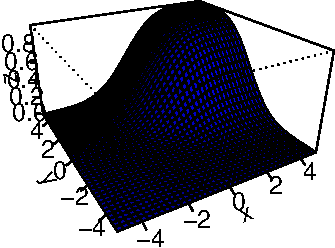
\includegraphics{./02-Review-Prob_n_Stats_files/figure-pdf/unnamed-chunk-2-1.pdf}

}

\end{figure}

\hypertarget{multidimensional-probability-function}{%
\subsubsection{Multidimensional Probability
Function}\label{multidimensional-probability-function}}

\textbf{Discrete random vectors:} \(X\) takes only countably many
(i.e.~discrete) values
\(\mathbf{x}_1,\mathbf{x}_2,\dots\in\mathbb{R}^d\) and has a
\textbf{multidimensional probability function}
\(p(\mathbf{x}_i)=P(X=\mathbf{x}_i)\) for \(i=1,2,\dots\). That is,
\begin{align*}
P(X\in [a_1,b_1]\times\dots\times [a_d,b_d])=
\sum_{\mathbf{x}_i\in [a_1,b_1]\times\dots\times [a_d,b_d]}p(\mathbf{x}_i).
\end{align*}

\hypertarget{multidimensional-density-function}{%
\subsubsection{Multidimensional Density
Function}\label{multidimensional-density-function}}

\textbf{Continuous random vectors:} \(X\) takes values in
\(\mathbb{R}^d\) and has a \textbf{multidimensional density function}
\(f(x_1,\dots,x_d)\). That is, \begin{align*}
P(X\in [a_1,b_1]\times\dots\times [a_d,b_d])=\int\limits_{a_d}^{b_d}\dots \int\limits _{a_1}^{b_1}f(x_1,\dots,x_d)dx_1\dots dx_d.
\end{align*} In the following we focus only on continuous random vectors
-- the discrete cases are treated analogously. Properties of
\textbf{multivariate density} functions:

\begin{itemize}
\tightlist
\item
  \(\displaystyle f(x_1,\dots,x_d)\geq 0\)

  \par
\item
  \(\displaystyle \int_{-\infty}^{\infty}\dots \int_{-\infty}^{\infty}f(x_1,\dots,x_d)dx_1\dots dx_d=1\)
\end{itemize}

\begin{Shaded}
\begin{Highlighting}[]
\DocumentationTok{\#\# Load the package}
\FunctionTok{library}\NormalTok{(mnormt)}

\NormalTok{x     }\OtherTok{\textless{}{-}} \FunctionTok{seq}\NormalTok{(}\SpecialCharTok{{-}}\DecValTok{5}\NormalTok{, }\DecValTok{5}\NormalTok{, }\FloatTok{0.25}\NormalTok{) }
\NormalTok{y     }\OtherTok{\textless{}{-}} \FunctionTok{seq}\NormalTok{(}\SpecialCharTok{{-}}\DecValTok{5}\NormalTok{, }\DecValTok{5}\NormalTok{, }\FloatTok{0.25}\NormalTok{)}
\NormalTok{mu    }\OtherTok{\textless{}{-}} \FunctionTok{c}\NormalTok{(}\DecValTok{0}\NormalTok{, }\DecValTok{0}\NormalTok{)}
\NormalTok{sigma }\OtherTok{\textless{}{-}} \FunctionTok{matrix}\NormalTok{(}\FunctionTok{c}\NormalTok{(}\DecValTok{2}\NormalTok{, }\SpecialCharTok{{-}}\DecValTok{1}\NormalTok{, }\SpecialCharTok{{-}}\DecValTok{1}\NormalTok{, }\DecValTok{2}\NormalTok{), }\AttributeTok{nrow =} \DecValTok{2}\NormalTok{)}
\NormalTok{f     }\OtherTok{\textless{}{-}} \ControlFlowTok{function}\NormalTok{(x, y) }\FunctionTok{dmnorm}\NormalTok{(}\FunctionTok{cbind}\NormalTok{(x, y), mu, sigma)}
\NormalTok{z     }\OtherTok{\textless{}{-}} \FunctionTok{outer}\NormalTok{(x, y, f)}

\FunctionTok{persp}\NormalTok{(x, y, z, }\AttributeTok{theta =} \SpecialCharTok{{-}}\DecValTok{30}\NormalTok{, }\AttributeTok{phi =} \DecValTok{25}\NormalTok{, }
      \AttributeTok{shade =} \FloatTok{0.75}\NormalTok{, }\AttributeTok{col =} \StringTok{"blue"}\NormalTok{, }\AttributeTok{expand =} \FloatTok{0.5}\NormalTok{, }\AttributeTok{r =} \DecValTok{2}\NormalTok{, }
      \AttributeTok{ltheta =} \DecValTok{25}\NormalTok{, }\AttributeTok{ticktype =} \StringTok{"detailed"}\NormalTok{)}
\end{Highlighting}
\end{Shaded}

\begin{figure}[H]

{\centering 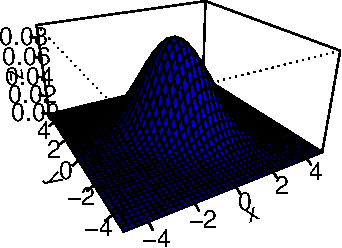
\includegraphics{./02-Review-Prob_n_Stats_files/figure-pdf/unnamed-chunk-3-1.pdf}

}

\end{figure}

\hypertarget{marginal-distribution-and-density-functions}{%
\subsubsection{Marginal Distribution and Density
Functions}\label{marginal-distribution-and-density-functions}}

Each random element, \(X_j\), with \(j=1,\dots,d\), of the random vector
\(X\) has its own \textbf{marginal distribution} \(F_j\). This is just
the univariate distribution of \(X_j\) when ignoring all other random
variables in \(X\). Formally we have:

\begin{itemize}
\tightlist
\item
  \textbf{Marginal distribution function:} \(F_j(x)=P(X_j\leq x)\)
\item
  \textbf{Marginal density function:} \(f_j\), for instance, for
  \(j=1\):
\end{itemize}

\$\$

f\_1(\{\color{blue}x\_1\})=\int\emph{\{-\infty\}\^{}\{\infty\}\dots \int}\{-\infty\}\^{}\{\infty\}f(\{\color{blue}x\_1\},x\_2\dots,
x\_d)dx\_2\dots  dx\_d

\$\$

\begin{figure}

{\centering 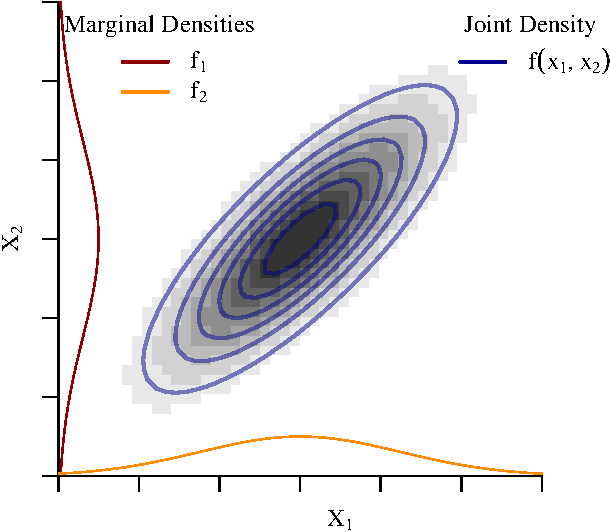
\includegraphics{./02-Review-Prob_n_Stats_files/figure-pdf/unnamed-chunk-4-1.pdf}

}

\end{figure}

\hypertarget{sec-condDistr}{%
\subsubsection{Conditional Distributions}\label{sec-condDistr}}

Often, we are interested in the \textbf{conditional distribution} of
\(X_j\) given certain values of all other random variables

\$\$

X\_1=x\_1,\ldots, X\_\{j-1\}=x\_\{j-1\},
X\_\{j+1\}=x\_\{j+1\},\ldots,X\_d=x\_d.

\[
That is, the distribution of $X_j$ when fixing the values of  
$X_1=x_1,\ldots,$ $X_{j-1}=x_{j-1},$ $X_{j+1}=x_{j+1},\ldots, X_d=x_d$.  An important tool is here the **conditional density** of, for instance, $X_1$ given $X_2=x_2,\ldots,X_d=x_d$:
\]

f(x\_1\mid x\_2,\ldots,x\_d)=\frac{f(x_1,x_2,\ldots,x_d)}{f_{X_{2},\ldots,X_{d}}(x_2,\ldots,x_d)},

\$\$ where \(f_{X_{2},\ldots,X_{d}}\) denotes the joint density of
\(X_2,\ldots,X_d\).

\begin{figure}

{\centering 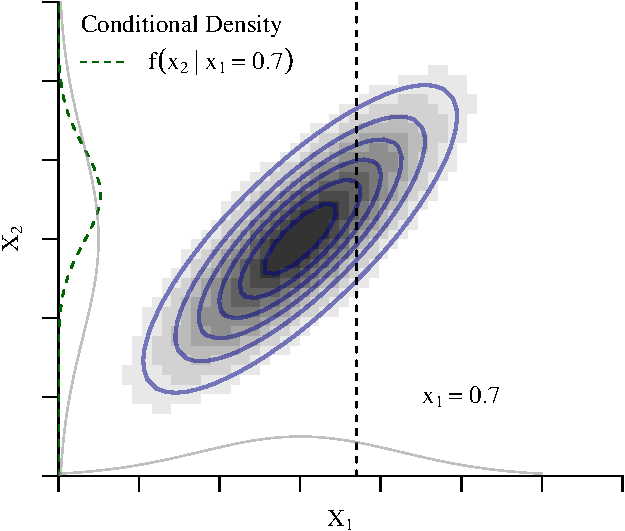
\includegraphics{./02-Review-Prob_n_Stats_files/figure-pdf/unnamed-chunk-5-1.pdf}

}

\end{figure}

\hypertarget{means-and-moments}{%
\subsection{Means and Moments}\label{means-and-moments}}

\hypertarget{unconditional-means}{%
\subsection{Unconditional Means}\label{unconditional-means}}

The \textbf{unconditional mean} of \(X_1\) is given by \$\$

E(X\_1)= \int x f\_\{X\_1\}(x)dx.

\[
The unconditional mean of a random vector $X=(X_1,\dots,X_d)'$ is given by the vector of element-wise means
\]

E(X)=(E(X\_1),\dots,E(X\_d))'.

\$\$

\hypertarget{conditional-means}{%
\subsection{Conditional Means}\label{conditional-means}}

Of central importance in \textbf{regression analysis} is the
\textbf{conditional mean}. The conditional mean of \(X_1\) for given
values \(X_2=x_2,\ldots,X_d=x_d\): \begin{align*}
  m(x_2,\dots,x_d):&=E(X_1|X_2=x_2,\ldots,X_d=x_d)\\
                   &= \int x_1 f(x_1\mid x_2,\ldots,x_d)dx_1,
\end{align*}\\
where \(m(x_2,\dots,x_d)\) denotes the \textbf{regression function}.

\hypertarget{means-of-transformed-random-variables-and-moments}{%
\subsection{Means of Transformed Random Variables and
Moments}\label{means-of-transformed-random-variables-and-moments}}

The \textbf{mean of a transformed random variable} \(r(X)\) is given by
\$\$

E(r(X))=\int r(x) f\_\{X\}(x)dx.

\$\$ Typical transformations are, for instance

\begin{itemize}
\tightlist
\item
  centering \(r(x)=x-E(X)\),
\item
  centering and scaling \(r(x)=(x-E(X))/\sqrt{Var(X)}\),
\item
  or \(r(x)=(x - E(X))^2\),
\end{itemize}

where the latter transformation leads to the \textbf{second central
moment}, i.e.~the variance of \(X\),
\(Var(X)=\int (x - E(X))^2 f_{X}(x)dx\).

\bigskip

\begin{itemize}
\tightlist
\item
  The \(k\)th, \(k>0\), moment is given by \$\$
\end{itemize}

\mu\emph{\{k\}=\mathrm{E}\left[X^{k}\right]=\int}\{-\infty\}\textsuperscript{\{+\infty\}x}\{k\}
f\_X(x)d x.

\$\$

\begin{itemize}
\tightlist
\item
  The \(k\)th, \(k>1\), central moment is given by \$\$
\end{itemize}

\mu\textsuperscript{c\_\{k\}=\mathrm{E}\left[(X-\mathrm{E}[X])}\{k\}\right{]}=\int\_\{-\infty\}\textsuperscript{\{+\infty\}(x-\mu)}\{k\}
f\_X(x)d x,

\$\$ where \(\mu=E(X)\).

\textbf{Note:} Moments determine the tail of a distribution (but not
much else); see Lindsay and Basak (2000). Roughly: The more moments a
distribution has the faster converge its tails to zero. Distributions
with compact supports (e.g.~the uniform distribution \(U[a,b]\)) have
infinitely many moments. The Normal distribution has also infinitely
many moments -- even though this distribution has not a compact support
since \(\phi(x)>0\) for all \(x\in\mathbb{R}\). .

\hypertarget{law-of-total-expectation}{%
\subsubsection{Law of Total
Expectation}\label{law-of-total-expectation}}

As long as we do not fix the values of the conditioning variables,
\(X_2,\dots,X_d\), they are random variables. Consequently, the
conditional mean is generally itself a random variable \$\$

E(X\_1\textbar X\_2,\ldots,X\_d)=\int x\_1
f(x\_1\mid X\_2,\ldots,X\_d)dx\_1.

\$\$ Note that \(f(x_1\mid X_2,\ldots,X_d)\) is just a transformation of
the random variables \(X_2,\dots,X_d\). So we can easily compute the
unconditional mean \(E(X_1)\) by taking the mean of
\(E(X_1|X_2,\ldots,X_d)\) as following, \begin{align*}
&E\big({\color{RedViolet}E(X_1|X_2,\ldots,X_d)}\big)=\\
&=\int\dots\int\;{\color{RedViolet}\int x_1 f(x_1\mid x_2,\ldots,x_d)dx_1}\;f_{X_2,\dots,X_d}(x_2,\ldots,x_d)dx_2\dots dx_d\\
&=\int x_1 \left(\int\dots\int f(x_1,{\color{blue}x_2,\ldots,x_d}){\color{blue}dx_2\dots dx_d}\right)dx_1\\
&=\int x_1 f_{X_1}(x_1)dx_1\\
&=E(X_1).
\end{align*}

The result that \(E\big(E(X_1|X_2,\ldots,X_d)\big)=E(X_1)\) is called
\textbf{law of total expectation} or \textbf{law of iterated
expectation}.

\hypertarget{independent-random-variables}{%
\subsection{Independent Random
Variables}\label{independent-random-variables}}

Random variables \(X_1,\dots,X_d\) are mutually \textbf{independent} if
for all \(x=(x_1,\dots,x_d)^\prime\) it is true that \begin{align*}
  F(x_1,\dots,x_d)&=F_1(x_1)\cdot F_2(x_2)\cdot\ldots\cdot F_d(x_d)\\
  f(x_1,\dots,x_d)&=f_1(x_1)\cdot f_2(x_2)\cdot\ldots\cdot f_d(x_d)
\end{align*}

The following holds true:

\begin{itemize}
\tightlist
\item
  Two real-valued random variables \(X\) and \(Y\) are independent from
  each other \textit{if and only if} the marginal density of \(X\)
  equals the conditional density of \(X\) given \(Y=y\) for all
  \(y\in\mathbb{R}\),
\end{itemize}

\[f_X(x)=f_{X|Y}(x\mid y)\quad \text{ for all } y\in\mathbb{R}.\]

Of course, the same statement applies to the marginal density of \(Y\)
given \(X=x\) for all \(x\in\mathbb{R}\). That is, \(X\) and \(Y\) are
two independent real-valued random variables \textit{if and only if}
\(f_Y(y)=f_{Y|X}(y\mid x)\) for all \(x\in\mathbb{R}.\) - If a
real-valued random variable \(X\) is independent from a real-valued
random variable \(Y\), then the conditional mean of \(X\) given \(Y=y\)
equals the unconditional mean of \(X\) for all \(y\in\mathbb{R}\)
(i.e.~the regression function becomes a constant)

\[E(X\mid Y=y)=E(X)\quad \text{ for all } y\in\mathbb{R}.\]

Of course, the same statement applies to the conditional mean of \(Y\)
given \(X=x\) for all \(x\in\mathbb{R};\) i.e., if \(X\) and \(Y\) are
two independent random variables, then
\(E(Y\mid X=x)=E(Y)\quad \text{ for all } x\in\mathbb{R}.\)\newline
\textbf{Cautionary note:} The properties that \(E(X\mid Y=y)=E(X)\) for
all \(y\in\mathbb{R}\) or that \(E(Y\mid X=x)=E(Y)\) for all
\(x\in\mathbb{R}\), do \textbf{not} imply that \(Y\) and \(X\) are
independent.

\hypertarget{i.i.d.-samples}{%
\subsection{I.I.D. Samples}\label{i.i.d.-samples}}

Tradition dictates that the sample size is denoted by the natural number
\(n\in\{1,2,\dots\}\). A random sample is a collection
\(X=(X_{1}, \ldots, X_{n})\) of random variables
\(X_{1}, \ldots, X_{n}\). If \(X_{1}, \ldots, X_{n}\) are all
\textbf{independent} from each other and if each random variable has the
same marginal distribution, we say that the random sample \$\$

X=(X\_\{1\}, \ldots, X\_\{n\}).

\$\$ is \textbf{i.i.d. (independent and identically distributed).}

\hypertarget{some-important-discrete-random-variables}{%
\subsection{Some Important Discrete Random
Variables}\label{some-important-discrete-random-variables}}

\hypertarget{the-discrete-uniform-distribution}{%
\subsubsection{The Discrete Uniform
Distribution}\label{the-discrete-uniform-distribution}}

Let \(k>1\) be a given integer. Suppose that \(X\) has probability mass
function given by \$\$

f(x)=\left\{

\begin{array}{ll}
1 / k & \text { for } x=1, \ldots, k \\
0 & \text { otherwise. }
\end{array}

\right.

\$\$ We say that \(X\) has a uniform distribution on
\(\{1, \ldots, k\}\).

\begin{Shaded}
\begin{Highlighting}[]
\FunctionTok{set.seed}\NormalTok{(}\DecValTok{51}\NormalTok{)}
\DocumentationTok{\#\# Set the parameter k}
\NormalTok{k }\OtherTok{\textless{}{-}} \DecValTok{10}
\DocumentationTok{\#\# Draw one realization from the discrete uniform distribution}
\FunctionTok{sample}\NormalTok{(}\AttributeTok{x =} \DecValTok{1}\SpecialCharTok{:}\NormalTok{k, }\AttributeTok{size =} \DecValTok{1}\NormalTok{, }\AttributeTok{replace =} \ConstantTok{TRUE}\NormalTok{)}
\end{Highlighting}
\end{Shaded}

\begin{verbatim}
[1] 7
\end{verbatim}

\hypertarget{the-bernoulli-distribution}{%
\subsubsection{The Bernoulli
Distribution}\label{the-bernoulli-distribution}}

Let \(X\) represent a possibly unfair coin flip. Then \(P(X=1)=p\) and
\(P(X=0)=1-p\) for some \(p \in[0,1]\). We say that \(X\) has a
Bernoulli distribution written \(X\sim\operatorname{Bernoulli }(p)\).
The probability function is \(f(x)=p^{x}(1-p)^{1-x}\) for
\(x \in\{0,1\}\)

\begin{Shaded}
\begin{Highlighting}[]
\FunctionTok{set.seed}\NormalTok{(}\DecValTok{51}\NormalTok{)}
\DocumentationTok{\#\# Set the parameter p}
\NormalTok{p }\OtherTok{\textless{}{-}} \FloatTok{0.25}
\DocumentationTok{\#\# Draw n realization from the discrete uniform distribution}
\NormalTok{n }\OtherTok{\textless{}{-}} \DecValTok{5}
\FunctionTok{sample}\NormalTok{(}\AttributeTok{x =} \FunctionTok{c}\NormalTok{(}\DecValTok{0}\NormalTok{,}\DecValTok{1}\NormalTok{), }\AttributeTok{size =}\NormalTok{ n, }\AttributeTok{prob =} \FunctionTok{c}\NormalTok{(}\DecValTok{1}\SpecialCharTok{{-}}\NormalTok{p, p), }\AttributeTok{replace=}\ConstantTok{TRUE}\NormalTok{)}
\end{Highlighting}
\end{Shaded}

\begin{verbatim}
[1] 1 0 0 1 0
\end{verbatim}

\begin{Shaded}
\begin{Highlighting}[]
\DocumentationTok{\#\# Alternatively:}
\DocumentationTok{\#\# (Bernoulli(p) equals Binomial(1,p))}
\FunctionTok{rbinom}\NormalTok{(}\AttributeTok{n =}\NormalTok{ n, }\AttributeTok{size =} \DecValTok{1}\NormalTok{, }\AttributeTok{prob =}\NormalTok{ p)}
\end{Highlighting}
\end{Shaded}

\begin{verbatim}
[1] 1 1 0 1 0
\end{verbatim}

\hypertarget{the-binomial-distribution}{%
\subsubsection{The Binomial
Distribution}\label{the-binomial-distribution}}

Suppose we have a coin which falls heads with probability \(p\) for some
\(p\in[0,1]\). Flip the coin \(n\) times and let \(X\) be the number of
heads (or successes). Assume that the tosses are independent. Let
\(f(x)=P(X=x)\) be the mass function. It can be shown that \$\$

f(x)=\left\{

\begin{array}{ll}
\left(\begin{array}{l}
n \\
x
\end{array}\right) p^{x}(1-p)^{n-x} & \text { for } x=0, \ldots, n \\
0 & \text { otherwise. }
\end{array}

\right.

\$\$ A random variable with this mas function is called a
\textbf{binomial random variable} and we write
\(X \sim \operatorname{Binomial}(n, p)\). If \(X_{1} \sim\) Binomial
\(\left(n_1, p1\right)\) and \(X_{2} \sim\)
Binomial\(\left(n_2, p\right)\) and if \(X_1\) and \(X_2\) are
independent, then
\(X_{1}+X_{2} \sim \operatorname{Binomial}\left(n_1+n_2, p\right)\)

\begin{Shaded}
\begin{Highlighting}[]
\FunctionTok{set.seed}\NormalTok{(}\DecValTok{51}\NormalTok{)}
\DocumentationTok{\#\# Set the parameters n and p}
\NormalTok{size }\OtherTok{\textless{}{-}}   \DecValTok{10} \CommentTok{\# number of trials}
\NormalTok{p    }\OtherTok{\textless{}{-}} \FloatTok{0.25} \CommentTok{\# prob of success}

\DocumentationTok{\#\# Draw n realization from the binomial distribution:}
\NormalTok{n }\OtherTok{\textless{}{-}} \DecValTok{5}
\FunctionTok{rbinom}\NormalTok{(}\AttributeTok{n =}\NormalTok{ n, }\AttributeTok{size =}\NormalTok{ size, }\AttributeTok{prob =}\NormalTok{ p)}
\end{Highlighting}
\end{Shaded}

\begin{verbatim}
[1] 4 1 2 6 1
\end{verbatim}

\hypertarget{some-important-continuous-random-variables}{%
\subsection{Some Important Continuous Random
Variables}\label{some-important-continuous-random-variables}}

\hypertarget{the-uniform-distribution}{%
\subsubsection{The Uniform
Distribution}\label{the-uniform-distribution}}

\(X\) has a \(\operatorname{Uniform}(a, b)\) distribution, written
\(X\sim \operatorname{Uniform}(a, b),\) if \$\$

f(x)=\left\{

\begin{array}{ll}
\frac{1}{b-a} & \text { for } x \in[a, b] \\
0 & \text { otherwise }
\end{array}

\right.

\[
where $a<b$. The distribution function is
\]

F(x)=\left\{

\begin{array}{ll}
0 & x<a \\
\frac{x-a}{b-a} & x \in[a, b] \\
1 & x>b
\end{array}

\right.

\$\$

\begin{Shaded}
\begin{Highlighting}[]
\DocumentationTok{\#\# Drawing from the uniform distribution:}
\NormalTok{n }\OtherTok{\textless{}{-}} \DecValTok{10}
\NormalTok{a }\OtherTok{\textless{}{-}} \DecValTok{0}
\NormalTok{b }\OtherTok{\textless{}{-}} \DecValTok{1}
\FunctionTok{runif}\NormalTok{(}\AttributeTok{n =}\NormalTok{ n, }\AttributeTok{min =}\NormalTok{ a, }\AttributeTok{max =}\NormalTok{ b)}
\end{Highlighting}
\end{Shaded}

\begin{verbatim}
 [1] 0.83442365 0.75138318 0.40601047 0.97101998 0.11233151 0.50750617
 [7] 0.69714201 0.17104008 0.25448233 0.01813812
\end{verbatim}

\hypertarget{the-normal-or-gaussian-distribution}{%
\subsubsection{The Normal (or Gaussian)
Distribution}\label{the-normal-or-gaussian-distribution}}

\(X\) has a Normal (or Gaussian) distribution with parameters \(\mu\)
and \(\sigma,\) denoted by \(X \sim N\left(\mu, \sigma^{2}\right),\) if
\$\$

f(x)=\frac{1}{\sigma \sqrt{2 \pi}}
\exp \left\{-\frac{1}{2 \sigma^{2}}(x-\mu)\^{}\{2\}\right\}, \quad x
\in \mathbb{R}

\$\$ where \(\mu \in \mathbb{R}\) and \(\sigma>0.\) Later we shall see
that \(\mu\) is the \say{center} (or mean of the distribution and
\(\sigma\) is the \say{spread} (or standard deviation) of the
distribution. The Normal plays an important role in probability and
statistics. Many phenomena in nature have approximately Normal
distributions. The \textbf{Central Limit Theorem} gives a special role
to the Normal distribution by stating that the distribution of averages
of random variables can be approximated by a Normal distribution.

We say that \(X\) has a standard Normal distribution if \(\mu=0\) and
\(\sigma=1\). Tradition dictates that a standard Normal random variable
is denoted by \(Z\). The PDF and CDF of a standard Normal are denoted by
\(\phi(z)\) and \(\Phi(z)\). There is no closed-form expression for
\(\Phi\). Here are some useful facts:

\begin{enumerate}
\def\labelenumi{(\roman{enumi})}
\item
  If \(X \sim N\left(\mu, \sigma^{2}\right)\) then
  \(Z=(X-\mu) / \sigma \sim N(0,1)\)
\item
  If \(Z \sim N(0,1)\) then
  \(X=\mu+\sigma Z \sim N\left(\mu, \sigma^{2}\right)\)
\item
  If
  \(X_{i} \sim N\left(\mu_{i}, \sigma_{i}^{2}\right), i=1, \ldots, n\)
  are independent then \$\$
\end{enumerate}

\sum\emph{\{i=1\}\^{}\{n\} X}\{i\}
\sim N\left(\sum\emph{\{i=1\}\^{}\{n\} \mu}\{i\},
\sum\emph{\{i=1\}\^{}\{n\} \sigma}\{i\}\^{}\{2\}\right).

\$\$

The following \textsf{R}-codes plots the standard Normal density
function: ::: \{.cell layout-align=``center''\}

\begin{Shaded}
\begin{Highlighting}[]
\CommentTok{\# draw a plot of the N(0,1) PDF}
\FunctionTok{curve}\NormalTok{(}\FunctionTok{dnorm}\NormalTok{(x),}
      \AttributeTok{xlim =} \FunctionTok{c}\NormalTok{(}\SpecialCharTok{{-}}\FloatTok{3.5}\NormalTok{, }\FloatTok{3.5}\NormalTok{),}
      \AttributeTok{ylab =} \StringTok{"Density"}\NormalTok{, }
      \AttributeTok{main =} \StringTok{"Standard Normal Density Function"}\NormalTok{) }
\end{Highlighting}
\end{Shaded}

\begin{figure}[H]

{\centering 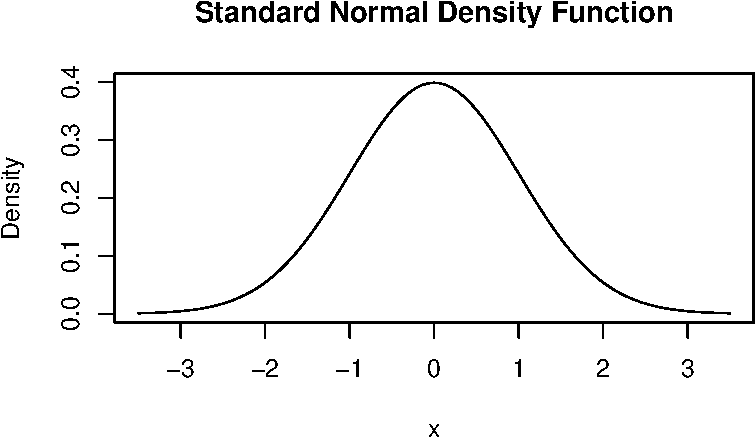
\includegraphics{./02-Review-Prob_n_Stats_files/figure-pdf/unnamed-chunk-10-1.pdf}

}

\end{figure}

:::

This is how you can draw realizations from pseudo random Normal
variables: ::: \{.cell\}

\begin{Shaded}
\begin{Highlighting}[]
\DocumentationTok{\#\# Drawing from the uniform distribution:}
\NormalTok{n     }\OtherTok{\textless{}{-}} \DecValTok{12}
\NormalTok{mu    }\OtherTok{\textless{}{-}} \DecValTok{0}
\NormalTok{sigma }\OtherTok{\textless{}{-}} \DecValTok{1}
\FunctionTok{rnorm}\NormalTok{(}\AttributeTok{n =}\NormalTok{ n, }\AttributeTok{mean =}\NormalTok{ mu, }\AttributeTok{sd =}\NormalTok{ sigma) }
\end{Highlighting}
\end{Shaded}

\begin{verbatim}
 [1]  0.085602504 -0.695791615 -1.364410561 -0.183503290 -1.675347076
 [6]  0.007303551  0.346965187  0.037914318  0.881345676 -0.882815597
[11] -0.883560071 -0.795629557
\end{verbatim}

:::

An extension of the normal distribution in a univariate setting is the
multivariate normal distribution. Let \(X=(X_1,\dots,X_k)'\) be a
\(k\)-dimensional normal variable, short \(X\sim N_k(\mu,\Sigma)\) with
mean vector \(E(X)=\mu\in\mathbb{R}^k\) and covariance matrix
\(\operatorname{Cov}(X)=\Sigma\). The joint density function or
\textbf{probability density function (pdf)} of the \(k\)-dimensional
multivariate normal distribution is \$\$

f\_\{X\}\left(x\_\{1\}, \ldots,
x\_\{k\}\right)=\frac{\exp \left(-\frac{1}{2}(x-\mu)' \Sigma^{-1}(x-\mu)\right)}{\sqrt{(2 \pi)^{k}|\Sigma|}},

\[
where $|\Sigma|$ denotes the determinant of $\Sigma$. For $k=2$ we have the bivariate pdf of two random normal variables, $X$ and $Y$ say
\begin{align*}
&g_{X,Y}(x,y) = \frac{1}{2\pi\sigma_X\sigma_Y\sqrt{1-\rho_{XY}^2}} \\ 
& \cdot \, \exp \left\{ \frac{1}{-2(1-\rho_{XY}^2)} \left[ \left( \frac{x-\mu_x}{\sigma_X} \right)^2 - 2\rho_{XY}\left( \frac{x-\mu_X}{\sigma_X} \right)\left( \frac{y-\mu_Y}{\sigma_Y} \right) + \left( \frac{y-\mu_Y}{\sigma_Y} \right)^2 \right]  \right\}.
\end{align*}
Lets consider the special case where $X$ and $Y$ are independent standard normal random variables with densities $f_X(x)$ and $f_Y(y)$. We then have the parameters $\sigma_X = \sigma_Y = 1$, $\mu_X=\mu_Y=0$ (due to marginal standard normality) and correlation $\rho_{XY}=0$ (due to independence). The joint density of $X$ and $Y$ then becomes
\]

g\_\{X,Y\}(x,y) = f\_X(x) f\_Y(y) = \frac{1}{2\pi} \cdot \exp \left\{
-\frac{1}{2}\left[x^2 + y^2\right]\right\}.

\$\$

\hypertarget{sec-chisqdist}{%
\subsubsection{The Chi-Squared Distribution}\label{sec-chisqdist}}

The chi-squared distribution is another distribution relevant in
econometrics. It is often needed when testing special types of
hypotheses frequently encountered when dealing with regression models.

The sum of \(M\) squared \emph{independent standard normal} distributed
random variables, \(Z_1,\dots,Z_M\) follows a chi-squared distribution
with \(M\) degrees of freedom: \begin{align*}
Z_1^2 + \dots + Z_M^2 = \sum_{m=1}^M Z_m^2 \sim \chi^2_M. 
\end{align*} A \(\chi^2\) distributed random variable with \(M\) degrees
of freedom has expectation \(M\), mode at \(M-2\) for \(M \geq 2\) and
variance \(2 \cdot M\).

Using the code below, we can display the pdf and the distribution
function or \textbf{cumulated density function (cdf)} of a \(\chi^2_3\)
random variable in a single plot. This is achieved by setting the
argument \texttt{add\ =\ TRUE"} in the second call of
\texttt{"curve()"}. Further we adjust limits of both axes using
\texttt{"xlim"} and \texttt{"ylim"} and choose different colors to make
both functions better distinguishable. The plot is completed by adding a
legend with help of \texttt{"legend()"}.

\begin{Shaded}
\begin{Highlighting}[]
\CommentTok{\# plot the PDF}
\FunctionTok{curve}\NormalTok{(}\FunctionTok{dchisq}\NormalTok{(x, }\AttributeTok{df =} \DecValTok{3}\NormalTok{), }
      \AttributeTok{xlim =} \FunctionTok{c}\NormalTok{(}\DecValTok{0}\NormalTok{, }\DecValTok{10}\NormalTok{), }
      \AttributeTok{ylim =} \FunctionTok{c}\NormalTok{(}\DecValTok{0}\NormalTok{, }\DecValTok{1}\NormalTok{), }
      \AttributeTok{col =} \StringTok{"blue"}\NormalTok{,}
      \AttributeTok{ylab =} \StringTok{""}\NormalTok{,}
      \AttributeTok{main =} \StringTok{"pdf and cdf of Chi{-}Squared Distribution, M = 3"}\NormalTok{)}

\CommentTok{\# add the CDF to the plot}
\FunctionTok{curve}\NormalTok{(}\FunctionTok{pchisq}\NormalTok{(x, }\AttributeTok{df =} \DecValTok{3}\NormalTok{), }
      \AttributeTok{xlim =} \FunctionTok{c}\NormalTok{(}\DecValTok{0}\NormalTok{, }\DecValTok{10}\NormalTok{), }
      \AttributeTok{add =} \ConstantTok{TRUE}\NormalTok{, }
      \AttributeTok{col =} \StringTok{"red"}\NormalTok{)}

\CommentTok{\# add a legend to the plot}
\FunctionTok{legend}\NormalTok{(}\StringTok{"topleft"}\NormalTok{, }
       \FunctionTok{c}\NormalTok{(}\StringTok{"PDF"}\NormalTok{, }\StringTok{"CDF"}\NormalTok{), }
       \AttributeTok{col =} \FunctionTok{c}\NormalTok{(}\StringTok{"blue"}\NormalTok{, }\StringTok{"red"}\NormalTok{), }
       \AttributeTok{lty =} \FunctionTok{c}\NormalTok{(}\DecValTok{1}\NormalTok{, }\DecValTok{1}\NormalTok{))}
\end{Highlighting}
\end{Shaded}

\begin{figure}[H]

{\centering 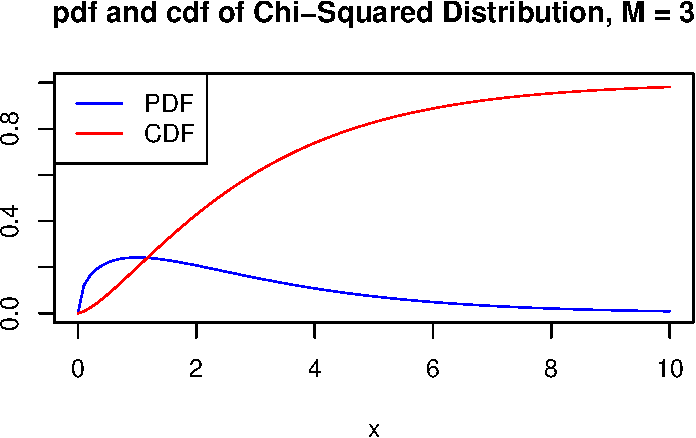
\includegraphics{./02-Review-Prob_n_Stats_files/figure-pdf/unnamed-chunk-12-1.pdf}

}

\end{figure}

Since the outcomes of a \(\chi^2_M\) distributed random variable are
always positive, the support of the related PDF and CDF is
\(\mathbb{R}_{\geq0}\).

As expectation and variance depend (solely!) on the degrees of freedom,
the distribution's shape changes drastically if we vary the number of
squared standard normals that are summed up. This relation is often
depicted by overlaying densities for different \(M\), see the Wikipedia
Article.

We reproduce this here by plotting the density of the \(\chi_1^2\)
distribution on the interval \([0,15]\) with \texttt{"curve()"}. In the
next step, we loop over degrees of freedom \(M=2,...,7\) and add a
density curve for each \(M\) to the plot. We also adjust the line color
for each iteration of the loop by setting \texttt{"col\ =\ M"}. At last,
we add a legend that displays degrees of freedom and the associated
colors.

\begin{Shaded}
\begin{Highlighting}[]
\CommentTok{\# plot the density for M=1}
\FunctionTok{curve}\NormalTok{(}\FunctionTok{dchisq}\NormalTok{(x, }\AttributeTok{df =} \DecValTok{1}\NormalTok{), }
      \AttributeTok{xlim =} \FunctionTok{c}\NormalTok{(}\DecValTok{0}\NormalTok{, }\DecValTok{15}\NormalTok{), }
      \AttributeTok{xlab =} \StringTok{"x"}\NormalTok{, }
      \AttributeTok{ylab =} \StringTok{"Density"}\NormalTok{, }
      \AttributeTok{main =} \StringTok{"Chi{-}Square Distributed Random Variables"}\NormalTok{)}

\CommentTok{\# add densities for M=2,...,7 to the plot using a \textquotesingle{}for()\textquotesingle{} loop }
\ControlFlowTok{for}\NormalTok{ (M }\ControlFlowTok{in} \DecValTok{2}\SpecialCharTok{:}\DecValTok{7}\NormalTok{) \{}
  \FunctionTok{curve}\NormalTok{(}\FunctionTok{dchisq}\NormalTok{(x, }\AttributeTok{df =}\NormalTok{ M),}
        \AttributeTok{xlim =} \FunctionTok{c}\NormalTok{(}\DecValTok{0}\NormalTok{, }\DecValTok{15}\NormalTok{), }
        \AttributeTok{add =}\NormalTok{ T, }
        \AttributeTok{col =}\NormalTok{ M)}
\NormalTok{\}}

\CommentTok{\# add a legend}
\FunctionTok{legend}\NormalTok{(}\StringTok{"topright"}\NormalTok{, }
       \FunctionTok{as.character}\NormalTok{(}\DecValTok{1}\SpecialCharTok{:}\DecValTok{7}\NormalTok{), }
       \AttributeTok{col =} \DecValTok{1}\SpecialCharTok{:}\DecValTok{7}\NormalTok{ , }
       \AttributeTok{lty =} \DecValTok{1}\NormalTok{, }
       \AttributeTok{title =} \StringTok{"D.F."}\NormalTok{)}
\end{Highlighting}
\end{Shaded}

\begin{figure}[H]

{\centering 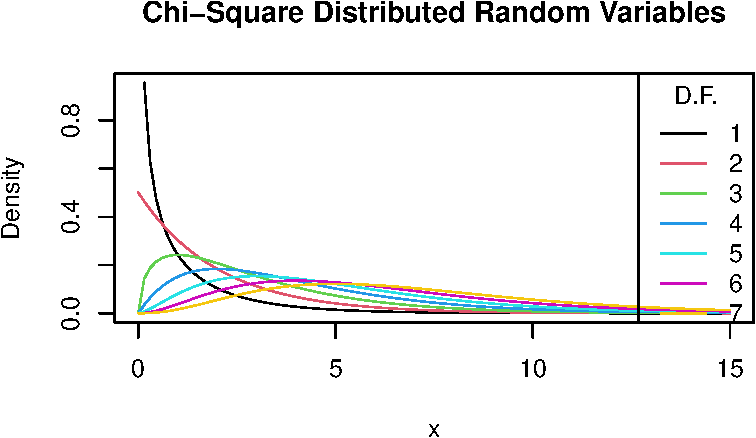
\includegraphics{./02-Review-Prob_n_Stats_files/figure-pdf/unnamed-chunk-13-1.pdf}

}

\end{figure}

Increasing the degrees of freedom shifts the distribution to the right
(the mode becomes larger) and increases the dispersion (the
distribution's variance grows).

\hypertarget{the-student-t-distribution}{%
\subsubsection{The Student t
Distribution}\label{the-student-t-distribution}}

Let \(Z\) be a standard normal random variable, \(W\) a \(\chi^2_\nu\)
random variable and further assume that \(Z\) and \(W\) are independent.
Then it holds that \$\$

\frac{Z}{\sqrt{W/\nu}} =:X \sim t\_\nu

\$\$ and \(X\) follows a \emph{Student \(t\) distribution} (or simply
\(t\) distribution) with \(\nu\) degrees of freedom.

The shape of a \(t_\nu\) distribution depends on \(\nu\). \(t\)
distributions are symmetric, bell-shaped and look similar to a normal
distribution, especially when \(\nu\) is large. This is not a
coincidence: for a sufficiently large \(\nu\), the \(t_\nu\)
distribution can be approximated by the standard normal distribution.
This approximation works reasonably well for \(\nu\geq 30\).

A \(t_\nu\) distributed random variable \(X\) has an expectation if
\(\nu>1\) and it has a variance if \(\nu>2\). \begin{align*}
  E(X) =& 0, \ M>1 \\
  \text{Var}(X) =& \frac{M}{M-2}, \ M>2
\end{align*}

Let us plot some \(t\) distributions with different degrees of freedoms
\(\nu\) and compare them to the standard normal distribution.

\begin{Shaded}
\begin{Highlighting}[]
\CommentTok{\# plot the standard normal density}
\FunctionTok{curve}\NormalTok{(}\FunctionTok{dnorm}\NormalTok{(x), }
      \AttributeTok{xlim =} \FunctionTok{c}\NormalTok{(}\SpecialCharTok{{-}}\DecValTok{4}\NormalTok{, }\DecValTok{4}\NormalTok{), }
      \AttributeTok{xlab =} \StringTok{"x"}\NormalTok{, }
      \AttributeTok{lty =} \DecValTok{2}\NormalTok{, }
      \AttributeTok{ylab =} \StringTok{"Density"}\NormalTok{, }
      \AttributeTok{main =} \StringTok{"Densities of t Distributions"}\NormalTok{)}

\CommentTok{\# plot the t density for M=2}
\FunctionTok{curve}\NormalTok{(}\FunctionTok{dt}\NormalTok{(x, }\AttributeTok{df =} \DecValTok{2}\NormalTok{), }
      \AttributeTok{xlim =} \FunctionTok{c}\NormalTok{(}\SpecialCharTok{{-}}\DecValTok{4}\NormalTok{, }\DecValTok{4}\NormalTok{), }
      \AttributeTok{col =} \DecValTok{2}\NormalTok{, }
      \AttributeTok{add =}\NormalTok{ T)}

\CommentTok{\# plot the t density for M=4}
\FunctionTok{curve}\NormalTok{(}\FunctionTok{dt}\NormalTok{(x, }\AttributeTok{df =} \DecValTok{4}\NormalTok{), }
      \AttributeTok{xlim =} \FunctionTok{c}\NormalTok{(}\SpecialCharTok{{-}}\DecValTok{4}\NormalTok{, }\DecValTok{4}\NormalTok{), }
      \AttributeTok{col =} \DecValTok{3}\NormalTok{, }
      \AttributeTok{add =}\NormalTok{ T)}

\CommentTok{\# plot the t density for M=25}
\FunctionTok{curve}\NormalTok{(}\FunctionTok{dt}\NormalTok{(x, }\AttributeTok{df =} \DecValTok{25}\NormalTok{), }
      \AttributeTok{xlim =} \FunctionTok{c}\NormalTok{(}\SpecialCharTok{{-}}\DecValTok{4}\NormalTok{, }\DecValTok{4}\NormalTok{), }
      \AttributeTok{col =} \DecValTok{4}\NormalTok{, }
      \AttributeTok{add =}\NormalTok{ T)}

\CommentTok{\# add a legend}
\FunctionTok{legend}\NormalTok{(}\StringTok{"topright"}\NormalTok{, }
       \FunctionTok{c}\NormalTok{(}\StringTok{"N(0, 1)"}\NormalTok{, }\StringTok{"M=2"}\NormalTok{, }\StringTok{"M=4"}\NormalTok{, }\StringTok{"M=25"}\NormalTok{), }
       \AttributeTok{col =} \DecValTok{1}\SpecialCharTok{:}\DecValTok{4}\NormalTok{, }
       \AttributeTok{lty =} \FunctionTok{c}\NormalTok{(}\DecValTok{2}\NormalTok{, }\DecValTok{1}\NormalTok{, }\DecValTok{1}\NormalTok{, }\DecValTok{1}\NormalTok{))}
\end{Highlighting}
\end{Shaded}

\begin{figure}[H]

{\centering 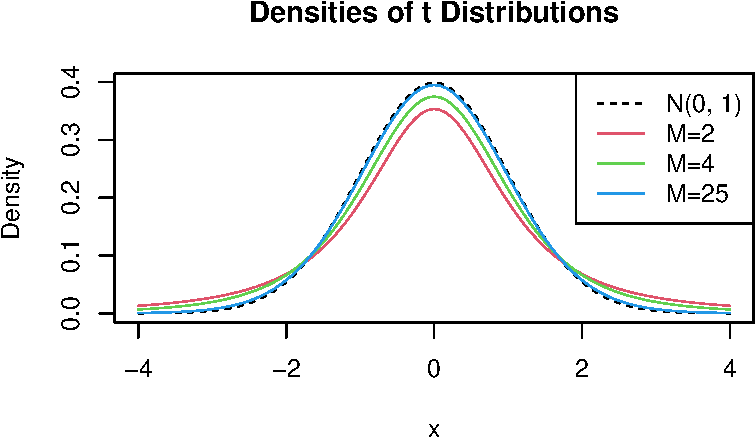
\includegraphics{./02-Review-Prob_n_Stats_files/figure-pdf/unnamed-chunk-14-1.pdf}

}

\end{figure}

The plot illustrates that as the degrees of freedom increase, the shape
of the \(t\) distribution comes closer to that of a standard normal bell
curve. Already for \(\nu=25\) we find little difference to the standard
normal density. If \(\nu\) is small, we find the distribution to have
heavier tails than a standard normal.

\hypertarget{cauchy-distribution}{%
\subsubsection{Cauchy Distribution}\label{cauchy-distribution}}

The Cauchy distribution is a special case of the \(t\) distribution
corresponding to \(\nu=1\). The density is \$\$

f(x)=\frac{1}{\pi\left(1+x^{2}\right)}.

\[
<!-- To see that this is indeed a density, let's do the integral: -->
<!-- \] --\textgreater{}

For the Cauchy distribution, the \textbf{expectation does not exist} --
that is, it has no mean. Let's try to compute the mean of a Cauchy
distribution and see what goes wrong. Its mean should be \$\$

\mu=E(X)=\int\_\{-\infty\}\^{}\{\infty\}
\frac{x d x}{\pi\left(1+x^{2}\right)}.

\[
In order for this improper integral to exist, we need both integrals $\int_{-\infty}^{0}$ and $\int_{0}^{\infty}$ to be finite. Let's look at the second integral.
\]

\int\emph{\{0\}\^{}\{\infty\}
\frac{x d x}{\pi\left(1+x^{2}\right)}=\left.\frac{1}{2 \pi}
\log \left(1+x\^{}\{2\}\right)\right\textbar{}}\{0\}
\^{}\{\infty\}=\infty

\$\$ Similarly, the other integral, \(\int_{-\infty}^{0},\) is
\(-\infty\). Since they're not both finite, the integral
\(\int_{-\infty}^{\infty}\) doesn't exist. In other words
\(\infty-\infty\) is not a number. Thus, the Cauchy distribution has no
mean.

What this means in practice is that if you take a sample
\(x_{1}, x_{2}, \ldots, x_{n}\) from the Cauchy distribution, then the
average \(\bar{x}\) does not tend to a particular number. Instead, every
so often you will get such a huge number, either positive or negative,
that the average is overwhelmed by it.

\hypertarget{sec-Fdist}{%
\subsubsection{The F Distribution}\label{sec-Fdist}}

Another ratio of random variables important to econometricians is the
ratio of two independent \(\chi^2\) distributed random variables that
are divided by their degrees of freedom \(M\) and \(n\). The quantity

\[ \frac{W/M}{V/n} \sim F_{M,n} \ \ \text{with} \ \ W \sim \chi^2_M \ \ , \ \ V \sim \chi^2_n \]

follows an \(F\) distribution with numerator degrees of freedom \(M\)
and denominator degrees of freedom \(n\), denoted \(F_{M,n}\). The
distribution was first derived by George Snedecor but was named in honor
of \href{https://en.wikipedia.org/wiki/Ronald_Fisher}{Sir Ronald
Fisher}.

By definition, the support of both PDF and CDF of an \(F_{M,n}\)
distributed random variable is \(\mathbb{R}_{\geq0}\).

Say we have an \(F\) distributed random variable \(Y\) with numerator
degrees of freedom \(3\) and denominator degrees of freedom \(14\) and
are interested in \(P(Y \geq 2)\). This can be computed with help of the
function \texttt{"pf()"}. By setting the argument \texttt{"lower.tail"}
to \texttt{"FALSE"} we ensure that \textsf{R} computes
\(1- P(Y \leq 2)\), i.e,the probability mass in the tail right of \(2\).

\begin{Shaded}
\begin{Highlighting}[]
\FunctionTok{pf}\NormalTok{(}\DecValTok{2}\NormalTok{, }\AttributeTok{df1 =} \DecValTok{3}\NormalTok{, }\AttributeTok{df2 =} \DecValTok{14}\NormalTok{, }\AttributeTok{lower.tail =}\NormalTok{ F)}
\end{Highlighting}
\end{Shaded}

\begin{verbatim}
[1] 0.1603538
\end{verbatim}

We can visualize this probability by drawing a line plot of the related
density and adding a color shading with \texttt{"polygon()"}.

\begin{Shaded}
\begin{Highlighting}[]
\CommentTok{\# define coordinate vectors for vertices of the polygon}
\NormalTok{x }\OtherTok{\textless{}{-}} \FunctionTok{c}\NormalTok{(}\DecValTok{2}\NormalTok{, }\FunctionTok{seq}\NormalTok{(}\DecValTok{2}\NormalTok{, }\DecValTok{10}\NormalTok{, }\FloatTok{0.01}\NormalTok{), }\DecValTok{10}\NormalTok{)}
\NormalTok{y }\OtherTok{\textless{}{-}} \FunctionTok{c}\NormalTok{(}\DecValTok{0}\NormalTok{, }\FunctionTok{df}\NormalTok{(}\FunctionTok{seq}\NormalTok{(}\DecValTok{2}\NormalTok{, }\DecValTok{10}\NormalTok{, }\FloatTok{0.01}\NormalTok{), }\DecValTok{3}\NormalTok{, }\DecValTok{14}\NormalTok{), }\DecValTok{0}\NormalTok{)}

\CommentTok{\# draw density of F\_\{3, 14\}}
\FunctionTok{curve}\NormalTok{(}\FunctionTok{df}\NormalTok{(x ,}\DecValTok{3}\NormalTok{ ,}\DecValTok{14}\NormalTok{), }
      \AttributeTok{ylim =} \FunctionTok{c}\NormalTok{(}\DecValTok{0}\NormalTok{, }\FloatTok{0.8}\NormalTok{), }
      \AttributeTok{xlim =} \FunctionTok{c}\NormalTok{(}\DecValTok{0}\NormalTok{, }\DecValTok{10}\NormalTok{), }
      \AttributeTok{ylab =} \StringTok{"Density"}\NormalTok{,}
      \AttributeTok{main =} \StringTok{"Density Function"}\NormalTok{)}

\CommentTok{\# draw the polygon}
\FunctionTok{polygon}\NormalTok{(x, y, }\AttributeTok{col =} \StringTok{"orange"}\NormalTok{)}
\end{Highlighting}
\end{Shaded}

\begin{figure}[H]

{\centering 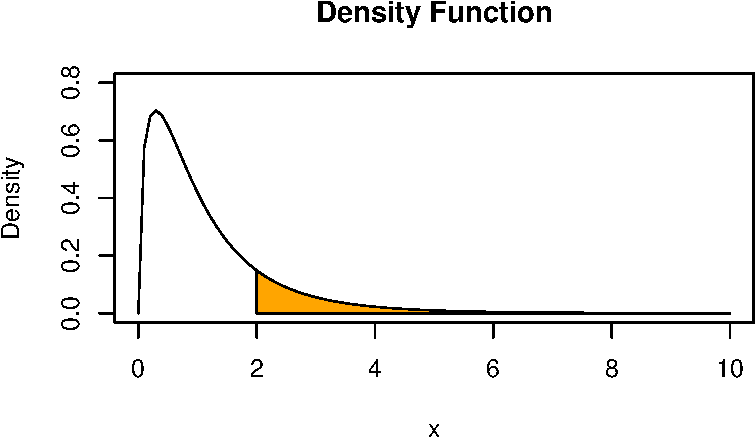
\includegraphics{./02-Review-Prob_n_Stats_files/figure-pdf/unnamed-chunk-16-1.pdf}

}

\end{figure}

The \(F\) distribution is related to many other distributions. An
important special case encountered in econometrics arises if the
denominator degrees of freedom are large such that the \(F_{M,n}\)
distribution can be approximated by the \(F_{M,\infty}\) distribution
which turns out to be simply the distribution of a \(\chi^2_M\) random
variable divided by its degrees of freedom \(M\), i.e.~ \$\$

W/M \sim F\_\{M,\infty\} \quad\text{with}\quad W \sim \chi\^{}2\_M.

\$\$

\bookmarksetup{startatroot}

\hypertarget{references}{%
\chapter*{References}\label{references}}
\addcontentsline{toc}{chapter}{References}

\bookmarksetup{startatroot}

\hypertarget{monte-carlo-simulations}{%
\chapter{Monte Carlo Simulations}\label{monte-carlo-simulations}}

In the following parts of the lecture, we will use Monte Carlo
simulations in oder to check whether a certain estimator is able to
estimate its (usually unknown) target parameter. In this chapter, we
will learn what Monte Carlo simulations are and how they can be
implemented.

\hypertarget{estimator-vs.-estimate}{%
\section{Estimator vs.~Estimate}\label{estimator-vs.-estimate}}

Let's assume that we have an iid random sample \(X_1,\dots,X_n\) with

\[
X_i\overset{iid}{\sim} F_X
\]

for all \(i=1,\dots,n\), and let \(\theta\in\mathbb{R}\) denote some
parameter (e.g.~the mean or the variance) of the distribution \(F_X\).

An \textbf{estimator} \(\hat\theta_n\) of \(\theta\) is a function of
the random sample \(X_1,\dots,X_n\),

\[
\hat\theta_n:=\hat\theta(X_1,\dots,X_n).
\]

Since \(\hat\theta_n\) is a function of the random variables
\(X_1,\dots,X_n\), the estimator \(\hat\theta_n\) is itself a
\textbf{random variable}.

The observed data \(X_{1,obs},\dots,X_{n,obs}\) is assumed to be a
certain realization of the random sample \(X_1,\dots,X_n\). The
corresponding \textbf{realization} of the estimator is called an
\textbf{estimate} of \(\theta\)

\[
\hat\theta_{n,obs}=\hat\theta(X_{1,obs},\dots,X_{n,obs}).
\]

\textbf{Note:} Often we do not use a distinguishing notation, but denote
both the estimator and its realization as \(\hat\theta_{n}\). This
ambiguity is often convenient since both points of views can make sense.

\textbf{Examples:}

\begin{itemize}
\tightlist
\item
  The sample mean as an estimator of the population mean:
\end{itemize}

\[
\hat\theta_n=\bar{X}_n=\frac{1}{n}\sum_{i=1}^nX_i \approx E(X_i) =\theta
\]

\begin{itemize}
\tightlist
\item
  The sample variance as an estimator of the population variance:
\end{itemize}

\[
\hat\theta_n=s_{UB}^2=\frac{1}{n-1}\sum_{i=1}^n\left(X_i - \bar{X}_n\right)^2 \approx Var(X_i) =\theta
\]

\hypertarget{deriving-the-distribution-of-estimators}{%
\section{Deriving the Distribution of
Estimators}\label{deriving-the-distribution-of-estimators}}

Usually, we do not know the distribution \(F_X\) of the random sample
\(X_1,\dots,X_n\) and thus do not know the distribution of the estimator
\(\hat\theta_n=\hat\theta(X_1,\dots,X_n)\). This is a fundamental
statistical problem and we need to overcome this problem in order to do
statistical inference (hypothesis testing, etc.). There are different
possibilities to derive/approximate the distribution of an estimator
\(\hat\theta_n\). In times when when computers were expensive,
statisticians mainly used mathematical derivations:

\begin{itemize}
\tightlist
\item
  \textbf{Mathematical Derivation using Distributional Assumptions.}
  Assuming a certain distribution \(F_X\) for the random sample
  \(X_1,\dots,X_n\) allows us to derive the \emph{exact} distribution of
  \(\hat\theta_n\) mathematically. (We consider this option in
  Chapter~\ref{sec-ssinf}.)

  \begin{itemize}
  \tightlist
  \item
    Pro: If the distributional assumption is correct, one has
    \emph{exact} inference for each sample size \(n\).
  \item
    Con: This option can fail miserably if the distributional assumption
    on \(F_X\) is wrong.
  \item
    Con: Such mathematical derivations are often only possible for
    particular distributions \(F_X\) like the normal distribution.
  \end{itemize}
\item
  \textbf{Mathematical Derivation using Asymptotic Statistics.} Large
  sample \((n\to\infty)\) approximations (i.e.~laws of large numbers and
  central limit theorems) allow us to derive the \emph{approximate}
  distribution of \(\hat\theta_n\). This option uses mathematical limit
  considerations by letting the sample size \(n\) diverge to infinity.
  (We consider this option in Chapter~\ref{sec-lsinf}.)

  \begin{itemize}
  \tightlist
  \item
    Pro: Only a few qualitative distributional assumptions are needed.
  \item
    Con: The derived asymptotic (\(n\to\infty\)) distribution is only
    exact for the practically impossible case where \(n=\infty\) and
    thus can fail to approximate the exact distribution of
    \(\hat\theta_n\) for given (finite) sample sizes \(n\); particularly
    if \(n\) is small.
  \end{itemize}
\end{itemize}

With computers, we have further options to approximate the exact
distribution of estimators using (pseudo-)random number generators. One
example are Monte Carlo simulations:

\begin{itemize}
\tightlist
\item
  \textbf{Monte Carlo Simulations.} Using (pseudo-)random number
  generators, we can draw \texttt{B} many realizations
\end{itemize}

\[
(X_{1,1,obs},\dots,X_{n,1,obs}),\; (X_{1,2,obs},\dots,X_{n,2,obs}),\dots, (X_{1,B,obs},\dots,X_{n,B,obs})
\]

of the random sample \(X_{1},\dots,X_{n}\) from basically any
distribution \(F_X\) and thus can compute \texttt{B} many realizations

\[
\underbrace{\hat\theta(X_{1,1,obs},\dots,X_{n,1,obs})}_{=\hat\theta_{n,1,obs}},\;\underbrace{\hat\theta(X_{1,2,obs},\dots,X_{n,2,obs})}_{=\hat\theta_{n,2,obs}},\dots,\underbrace{\hat\theta(X_{1,B,obs},\dots,X_{n,B,obs})}_{=\hat\theta_{n,B,obs}}
\]

of the estimator \(\hat\theta_n\). This set of realizations
\(\hat\theta_{n,1,obs},\dots,\hat\theta_{n,B,obs}\) allows us then to
approximate the exact distribution of \(\hat\theta_n\) for given sample
sizes \(n\) and given distributions \(F_X\). (We use this option to
validate theoretical statements in Chapter~\ref{sec-ssinf} and
Chapter~\ref{sec-lsinf}.) * Pro: Works for basically every
distributional assumption. * Con: This option can fail miserably if the
distributional assumption on \(F_X\) is wrong.

The following \texttt{R} code generates \texttt{B} many realizations of
the sample mean estimator \(\hat\theta_n=\bar{X}_n\) using a random
sample \(X_1,\dots,X_n\), where \(F_X\) is a normal distribution with
mean \((\theta=)\mu=10\) and variance \(\sigma^2=5\):

\begin{Shaded}
\begin{Highlighting}[]
\DocumentationTok{\#\# True parameter value }
\NormalTok{mu            }\OtherTok{\textless{}{-}} \DecValTok{10}
\DocumentationTok{\#\# Number of Monte Carlo repetitions:}
\NormalTok{B             }\OtherTok{\textless{}{-}} \DecValTok{10000}
\DocumentationTok{\#\# Sequence of different sample sizes:}
\NormalTok{n\_seq         }\OtherTok{\textless{}{-}} \FunctionTok{c}\NormalTok{(}\DecValTok{5}\NormalTok{, }\DecValTok{15}\NormalTok{, }\DecValTok{50}\NormalTok{)}


\DocumentationTok{\#\# \#\#\#\#\#\#\#\#\#\#\#\#\#\#\#\#\#\#\#\#\#\#\#\#\#\#\#\#\#\#\#\#\#\#\#\#\#\#}
\DocumentationTok{\#\# 1st Possibility: Using a for() loop \#\#}
\DocumentationTok{\#\# \#\#\#\#\#\#\#\#\#\#\#\#\#\#\#\#\#\#\#\#\#\#\#\#\#\#\#\#\#\#\#\#\#\#\#\#\#\#}

\DocumentationTok{\#\# Set seed for the random number generator to get reproducible results}
\FunctionTok{set.seed}\NormalTok{(}\DecValTok{3}\NormalTok{)}

\CommentTok{\# Container for the generated estimates:}
\NormalTok{estimates\_mat }\OtherTok{\textless{}{-}} \FunctionTok{matrix}\NormalTok{(}\ConstantTok{NA}\NormalTok{, }\AttributeTok{nrow =}\NormalTok{ B, }\AttributeTok{ncol =} \FunctionTok{length}\NormalTok{(n\_seq))}

\ControlFlowTok{for}\NormalTok{(j }\ControlFlowTok{in} \DecValTok{1}\SpecialCharTok{:}\FunctionTok{length}\NormalTok{(n\_seq))\{}
  \DocumentationTok{\#\# select the sample size}
\NormalTok{  n }\OtherTok{\textless{}{-}}\NormalTok{ n\_seq[j]}
  \ControlFlowTok{for}\NormalTok{(b }\ControlFlowTok{in} \DecValTok{1}\SpecialCharTok{:}\NormalTok{B)\{}
    \DocumentationTok{\#\# generate realization of the random sample }
\NormalTok{    X\_sample }\OtherTok{\textless{}{-}} \FunctionTok{rnorm}\NormalTok{(}\AttributeTok{n =}\NormalTok{ n, }\AttributeTok{mean =}\NormalTok{ mu, }\AttributeTok{sd =} \FunctionTok{sqrt}\NormalTok{(}\DecValTok{5}\NormalTok{))}
    \DocumentationTok{\#\# compute the sample mean and safe it}
\NormalTok{    estimates\_mat[b,j] }\OtherTok{\textless{}{-}} \FunctionTok{mean}\NormalTok{(X\_sample)}
\NormalTok{  \}}
\NormalTok{\}}

\DocumentationTok{\#\# \#\#\#\#\#\#\#\#\#\#\#\#\#\#\#\#\#\#\#\#\#\#\#\#\#\#\#\#\#\#\#\#\#\#\#\#\#}
\DocumentationTok{\#\# 2nd Possibility: Using replicate() \#\#}
\DocumentationTok{\#\# \#\#\#\#\#\#\#\#\#\#\#\#\#\#\#\#\#\#\#\#\#\#\#\#\#\#\#\#\#\#\#\#\#\#\#\#\#}

\DocumentationTok{\#\# Set seed for the random number generator to get reproducible results}
\FunctionTok{set.seed}\NormalTok{(}\DecValTok{3}\NormalTok{)}

\DocumentationTok{\#\# Function that generates estimator realizations }
\NormalTok{my\_estimates\_generator }\OtherTok{\textless{}{-}} \ControlFlowTok{function}\NormalTok{(n)\{}
\NormalTok{  X\_sample }\OtherTok{\textless{}{-}} \FunctionTok{rnorm}\NormalTok{(}\AttributeTok{n =}\NormalTok{ n, }\AttributeTok{mean =}\NormalTok{ mu, }\AttributeTok{sd =} \FunctionTok{sqrt}\NormalTok{(}\DecValTok{5}\NormalTok{))}
  \DocumentationTok{\#\# compute the sample mean realization}
  \FunctionTok{return}\NormalTok{(}\FunctionTok{mean}\NormalTok{(X\_sample))}
\NormalTok{\}}

\NormalTok{estimates\_mat }\OtherTok{\textless{}{-}} \FunctionTok{cbind}\NormalTok{(}
  \FunctionTok{replicate}\NormalTok{(B, }\FunctionTok{my\_estimates\_generator}\NormalTok{(}\AttributeTok{n =}\NormalTok{ n\_seq[}\DecValTok{1}\NormalTok{])),}
  \FunctionTok{replicate}\NormalTok{(B, }\FunctionTok{my\_estimates\_generator}\NormalTok{(}\AttributeTok{n =}\NormalTok{ n\_seq[}\DecValTok{2}\NormalTok{])),}
  \FunctionTok{replicate}\NormalTok{(B, }\FunctionTok{my\_estimates\_generator}\NormalTok{(}\AttributeTok{n =}\NormalTok{ n\_seq[}\DecValTok{3}\NormalTok{]))}
\NormalTok{)}
\end{Highlighting}
\end{Shaded}

Based on the \texttt{B}\(=10,000\) realizations of the estimator
\(\bar{X}_n\), we can compute histograms and non-parametric density
estimates to get an idea about the true distribution of \(\bar{X}_n\)
for the case of random samples \(X_1,\dots,X_n\) from a normal
distribution with mean \(\mu=10\) and variance \(\sigma^2=5\):

\begin{Shaded}
\begin{Highlighting}[]
\FunctionTok{par}\NormalTok{(}\AttributeTok{mfrow=}\FunctionTok{c}\NormalTok{(}\DecValTok{1}\NormalTok{,}\DecValTok{3}\NormalTok{))}
\FunctionTok{hist}\NormalTok{(estimates\_mat[,}\DecValTok{1}\NormalTok{], }\AttributeTok{main=}\StringTok{"n=5"}\NormalTok{, }\AttributeTok{xlab=}\StringTok{""}\NormalTok{,  }\AttributeTok{xlim =} \FunctionTok{range}\NormalTok{(estimates\_mat[,}\DecValTok{1}\NormalTok{]), }\AttributeTok{prob =} \ConstantTok{TRUE}\NormalTok{, }\AttributeTok{ylim =} \FunctionTok{c}\NormalTok{(}\DecValTok{0}\NormalTok{, }\FloatTok{1.2}\NormalTok{))}
\FunctionTok{lines}\NormalTok{(}\FunctionTok{density}\NormalTok{(estimates\_mat[,}\DecValTok{1}\NormalTok{], }\AttributeTok{bw =} \FunctionTok{bw.SJ}\NormalTok{(estimates\_mat[,}\DecValTok{1}\NormalTok{])), }\AttributeTok{col=}\StringTok{"blue"}\NormalTok{, }\AttributeTok{lwd=}\FloatTok{1.5}\NormalTok{)}
\FunctionTok{hist}\NormalTok{(estimates\_mat[,}\DecValTok{2}\NormalTok{], }\AttributeTok{main=}\StringTok{"n=15"}\NormalTok{, }\AttributeTok{xlab=}\StringTok{""}\NormalTok{, }\AttributeTok{xlim =} \FunctionTok{range}\NormalTok{(estimates\_mat[,}\DecValTok{1}\NormalTok{]), }\AttributeTok{prob =} \ConstantTok{TRUE}\NormalTok{, }\AttributeTok{ylim =} \FunctionTok{c}\NormalTok{(}\DecValTok{0}\NormalTok{, }\FloatTok{1.2}\NormalTok{))}
\FunctionTok{lines}\NormalTok{(}\FunctionTok{density}\NormalTok{(estimates\_mat[,}\DecValTok{2}\NormalTok{], }\AttributeTok{bw =} \FunctionTok{bw.SJ}\NormalTok{(estimates\_mat[,}\DecValTok{3}\NormalTok{])), }\AttributeTok{col=}\StringTok{"blue"}\NormalTok{, }\AttributeTok{lwd=}\FloatTok{1.5}\NormalTok{)}
\FunctionTok{hist}\NormalTok{(estimates\_mat[,}\DecValTok{3}\NormalTok{], }\AttributeTok{main=}\StringTok{"n=50"}\NormalTok{, }\AttributeTok{xlab=}\StringTok{""}\NormalTok{, }\AttributeTok{xlim =} \FunctionTok{range}\NormalTok{(estimates\_mat[,}\DecValTok{1}\NormalTok{]), }\AttributeTok{prob =} \ConstantTok{TRUE}\NormalTok{, }\AttributeTok{ylim =} \FunctionTok{c}\NormalTok{(}\DecValTok{0}\NormalTok{, }\FloatTok{1.2}\NormalTok{))}
\FunctionTok{lines}\NormalTok{(}\FunctionTok{density}\NormalTok{(estimates\_mat[,}\DecValTok{2}\NormalTok{], }\AttributeTok{bw =} \FunctionTok{bw.SJ}\NormalTok{(estimates\_mat[,}\DecValTok{3}\NormalTok{])), }\AttributeTok{col=}\StringTok{"blue"}\NormalTok{, }\AttributeTok{lwd=}\FloatTok{1.5}\NormalTok{)}
\end{Highlighting}
\end{Shaded}

\begin{figure}[H]

{\centering 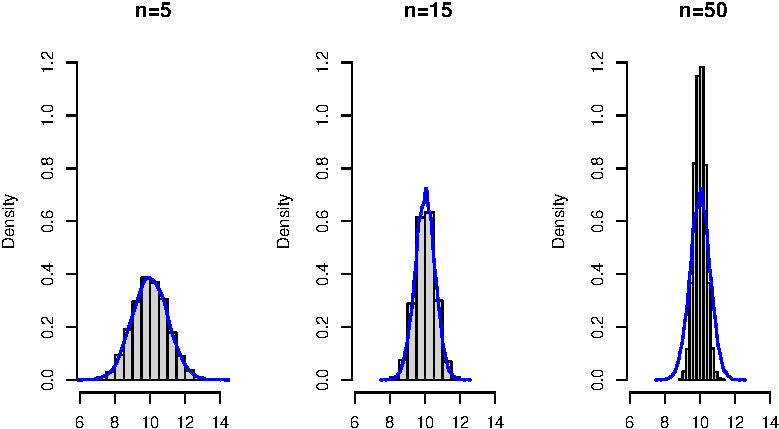
\includegraphics{./03-Monte-Carlo-Simulations_files/figure-pdf/fig-histdensplots-1.pdf}

}

\caption{\label{fig-histdensplots}Histrograms and non-parametric density
estimates of the distributions of the sample mean estimator for
different sample sizes.}

\end{figure}

Observations (Figure~\ref{fig-histdensplots}):

\begin{itemize}
\item
  At least on average, the estimates \(\bar{X}_n\) are close to the
  target parameter \(\mu=10\) for each sample size \(n\in\{5,15,50\}\).
  This feature of the estimator's distribution is summarized by the
  \textbf{bias} (see next section) of an estimator.
\item
  As the sample size increases, the distributions of the estimators
  \(\bar{X}_n\) concentrate around the target parameter \(\mu=10\). This
  feature of the estimator's distribution is summarized by the
  \textbf{mean squared error} (see next section) of an estimator.
\end{itemize}

Thus here the quality of the estimator \(\bar{X}_n\) gets better as
\(n\) gets large. To describe the quality of estimators more compactly,
statisticians/econometricians use specific metrics like bias, variance
and the mean squared error of the distribution of a estimator
\(\hat\theta\).

\hypertarget{assessing-the-quality-of-estimators}{%
\section{Assessing the Quality of
Estimators}\label{assessing-the-quality-of-estimators}}

Any reasonable estimator \(\hat\theta_n\) should be able to approximate
the (usually unknown) parameter value \(\theta\),

\[
\hat\theta_n\approx\theta,
\]

and the approximation should get better as the sample size increases
(i.e.~as \(n\to\infty\)).

Statisticians and econometricians use different metrics to assess the
approximation quality of an estimator \(\hat\theta_n\). The most
prominent metrics are bias, variance, and mean squared error.

\leavevmode\vadjust pre{\hypertarget{def-bias}{}}%
\begin{definition}[Bias of \(\theta\)]\label{def-bias}

The \textbf{bias} of an estimator \(\hat\theta_n\) is defined as

\[
\operatorname{Bias}\left(\hat\theta_n\right) = E\left(\hat\theta_n\right) - \theta.
\]

\end{definition}

We would like to have unbiased estimators
\(\operatorname{Bias}\left(\hat\theta_n\right)=0\) or at least
asymptotically unbiased estimators
\(\lim_{n\to\infty}\operatorname{Bias}\left(\hat\theta_n\right)=0\). If
the bias of an estimator is small (or zero), we know that the estimator
will have a distribution that is centered around the true (usually
unknown) parameter \(\theta\); however, such an estimator may still vary
a lot around \(\theta\). Therefore, is is also important to assess the
variance of the estimator.

\leavevmode\vadjust pre{\hypertarget{def-var}{}}%
\begin{definition}[Variance and Standard Error of
\(\theta\)]\label{def-var}

The \textbf{variance} of an estimator \(\hat\theta_n\) is defined
equivalently to the variance of any other random variable

\[
Var\left(\hat\theta_n\right) = E\left[\left(\hat\theta_n - E(\hat\theta_n)\right)^2\right].
\]

The square root of the variance of an estimator is called
\textbf{standard error} (not standard deviation) of \(\hat\theta_n\),

\[
\operatorname{SE}\left(\hat\theta_n\right) = \sqrt{Var\left(\hat\theta_n\right)}.
\]

\end{definition}

We would like to have estimators with a small as possible variance, and
the variance should decline as the sample size increases, such that
\(\lim_{n\to\infty}Var\left(\hat\theta_n\right)=0\).

\leavevmode\vadjust pre{\hypertarget{def-mse}{}}%
\begin{definition}[Mean Squared Error of \(\theta\)]\label{def-mse}

The \textbf{mean squared error} of an estimator \(\hat\theta_n\) is
defined as

\[
\operatorname{MSE}\left(\hat\theta_n\right) =  E\left[\left(\hat\theta_n - \theta\right)^2\right].
\]

\end{definition}

We would like to have estimators with a small as possible mean squared
error, and the mean squared error should decline as the sample size
increases, such that
\(\lim_{n\to\infty}\operatorname{MSE}\left(\hat\theta_n\right)=0\).

The following holds true:

\begin{itemize}
\tightlist
\item
  The mean squared error equals the sum of the squared bias and the
  variance:
\end{itemize}

\[
\operatorname{MSE}\left(\hat\theta_n\right) = \left(\operatorname{Bias}\left(\hat\theta_n\right)\right)^2 +  Var\left(\hat\theta_n\right) 
\]

\begin{itemize}
\tightlist
\item
  For unbiased estimators (i.e.~\(E(\hat\theta_n)=\theta\)) the mean
  squared error equals the variance, i.e.
\end{itemize}

\[
\underbrace{E\left[\left(\hat\theta_n - \theta\right)^2\right]}_{\operatorname{MSE}\left(\hat\theta_n\right)} = \underbrace{E\left[\left(\hat\theta_n - E\left(\hat\theta_n\right)\right)^2\right]}_{ Var\left(\hat\theta_n\right)} 
\]

Unfortunately, it is often difficult to derive the above assessment
metrics for given sample sizes \(n\) and given data distributions
\(F_X\). Monte Carlo simulations allow us to solve this issue.

\hypertarget{approximating-bias-variance-and-mean-squared-error-using-monte-carlo-simulations}{%
\section{Approximating Bias, Variance, and Mean Squared Error using
Monte Carlo
Simulations}\label{approximating-bias-variance-and-mean-squared-error-using-monte-carlo-simulations}}

We can use Monte Carlo simulations to approximate the assessment metrics
\(\operatorname{Bias}\left(\hat\theta_n\right),\)
\(Var\left(\hat\theta_n\right),\) and
\(\operatorname{MSE}\left(\hat\theta_n\right)\) for given sample sizes
\(n\) and given data distributions \(F_X\) with arbitrary precision.

Any of the the above assessment metrics require us to compute means of
random variables:

\begin{itemize}
\item
  For the \(\operatorname{Bias}\left(\hat\theta_n\right)\) we need to
  compute \(E\left(\hat\theta_n\right)-\theta\)
\item
  For the \(Var\left(\hat\theta_n\right)\) we need to compute
  \(E\left[\left(\hat\theta_n - E(\hat\theta_n)\right)^2\right]\).
\item
  For the \(\operatorname{MSE}\left(\hat\theta_n\right)\) we need to
  compute \(E\left[\left(\hat\theta_n - \theta\right)^2\right]\).
\end{itemize}

A Monte Carlo simulation can approximate these means by using the
\textbf{law of large numbers} which states that a sample mean over iid
random variables is able to approximate the population mean of these
random variables as the number of random variables to average over get
large.\footnote{Take a look at this visualization:
  \url{https://rpsychologist.com/d3/ci/}}

Thus, to compute a very precise approximation to
\(E\left(\hat\theta_n\right)-\theta\), we can use a computer to execute
the following algorithm:

\textbf{Step 1.} Generate \(B\) many (e.g.~\(B=10,000\)) realizations of
the iid random sample

\[
(X_{1,1},\dots,X_{n,1}),\; (X_{1,2},\dots,X_{n,2}),\dots, (X_{1,B},\dots,X_{n,B})
\]

\textbf{Step 2.} Compute the corresponding \(B\) many realizations of
the estimator

\[
\underbrace{\hat\theta(X_{1,1},\dots,X_{n,1})}_{=\hat\theta_{n,1}},\;\underbrace{\hat\theta(X_{1,2},\dots,X_{n,2})}_{=\hat\theta_{n,2}},\dots,\underbrace{\hat\theta(X_{1,B},\dots,X_{n,B})}_{=\hat\theta_{n,B}}
\]

\textbf{Step 3.} Use the sample mean as an approximation to the
population mean

\[
\left(\frac{1}{B}\sum_{b=1}^B \hat\theta_{n,b}\right) - \theta \approx E\left(\hat\theta_n\right)-\theta
\]

By law of large numbers this approximation gets arbitrarily precise as
\(B \to \infty\).

\begin{itemize}
\tightlist
\item
  The bias of \(\hat\theta_n\) can be approximated by
\end{itemize}

\[
\operatorname{Bias}\left(\hat\theta_n\right)=E\left(\hat\theta_n\right)-\theta\approx\left(\frac{1}{B}\sum_{b=1}^B \hat\theta_{n,b}\right) - \theta
\]

\begin{itemize}
\tightlist
\item
  The variance of \(\hat\theta_n\) can be approximated by
\end{itemize}

\[
Var\left(\hat\theta_n\right)=E\left[\left(\hat\theta_n - E(\hat\theta_n)\right)^2\right]\approx \frac{1}{B}\sum_{b=1}^B \left(\hat\theta_{n,b} - \left(\frac{1}{B}\sum_{b=1}^B \hat\theta_{n,b}\right)\right)^2
\]

\begin{itemize}
\tightlist
\item
  The mean squared error of \(\hat\theta_n\) can be approximated by
\end{itemize}

\[
\operatorname{MSE}\left(\hat\theta_n\right)=E\left[\left(\hat\theta_n - \theta\right)^2\right]\approx\frac{1}{B}\sum_{b=1}^B \left(\hat\theta_{n,b} - \theta\right)^2
\]

\hypertarget{example-sample-mean}{%
\subsection*{Example: Sample Mean}\label{example-sample-mean}}
\addcontentsline{toc}{subsection}{Example: Sample Mean}

The following \texttt{R} code contains a Monte Carlo simulation (
\texttt{B\ =\ 10000} replications) computing the bias, variance, and
means squared error for the sample mean
\((\hat\theta_n=)\bar{X}_n=\sum_{i=1}^nX_i\) as the estimator of the
population mean \((\theta=)\mu\). The random sample
\(X_i\overset{iid}{\sim}F_X\), \(i=1,\dots,n\), is drawn from a normal
distribution \(F_X=\mathcal{N}(\mu,\sigma^2)\) with mean \(\mu=10\) and
variance \(\sigma^2=5\). We investigate the accuracy of the estimator
for different sample sizes \(n\in\{5,15,50\}\).

\begin{Shaded}
\begin{Highlighting}[]
\DocumentationTok{\#\# Set seed for the random number generator to get reproducible results}
\FunctionTok{set.seed}\NormalTok{(}\DecValTok{3}\NormalTok{)}
\DocumentationTok{\#\# True parameter value (\textquotesingle{}theta\textquotesingle{} here \textquotesingle{}mu\textquotesingle{})}
\NormalTok{mu            }\OtherTok{\textless{}{-}} \DecValTok{10}
\DocumentationTok{\#\# Number of Monte Carlo repetitions:}
\NormalTok{B             }\OtherTok{\textless{}{-}} \DecValTok{10000}
\DocumentationTok{\#\# Sequence of different sample sizes:}
\NormalTok{n\_seq         }\OtherTok{\textless{}{-}} \FunctionTok{c}\NormalTok{(}\DecValTok{5}\NormalTok{, }\DecValTok{15}\NormalTok{, }\DecValTok{50}\NormalTok{)}

\DocumentationTok{\#\# Function that generates estimator realizations }
\NormalTok{my\_estimates\_generator }\OtherTok{\textless{}{-}} \ControlFlowTok{function}\NormalTok{(n)\{}
\NormalTok{  X\_sample }\OtherTok{\textless{}{-}} \FunctionTok{rnorm}\NormalTok{(}\AttributeTok{n =}\NormalTok{ n, }\AttributeTok{mean =}\NormalTok{ mu, }\AttributeTok{sd =} \FunctionTok{sqrt}\NormalTok{(}\DecValTok{5}\NormalTok{))}
  \DocumentationTok{\#\# compute the sample mean realization}
  \FunctionTok{return}\NormalTok{(}\FunctionTok{mean}\NormalTok{(X\_sample))}
\NormalTok{\}}

\NormalTok{estimates\_mat }\OtherTok{\textless{}{-}} \FunctionTok{cbind}\NormalTok{(}
  \FunctionTok{replicate}\NormalTok{(B, }\FunctionTok{my\_estimates\_generator}\NormalTok{(}\AttributeTok{n =}\NormalTok{ n\_seq[}\DecValTok{1}\NormalTok{])),}
  \FunctionTok{replicate}\NormalTok{(B, }\FunctionTok{my\_estimates\_generator}\NormalTok{(}\AttributeTok{n =}\NormalTok{ n\_seq[}\DecValTok{2}\NormalTok{])),}
  \FunctionTok{replicate}\NormalTok{(B, }\FunctionTok{my\_estimates\_generator}\NormalTok{(}\AttributeTok{n =}\NormalTok{ n\_seq[}\DecValTok{3}\NormalTok{]))}
\NormalTok{)}
\end{Highlighting}
\end{Shaded}

The following \texttt{R} code computes the Monte Carlo (MC)
approximations for the bias, variance, and mean squared error of
\(\bar{X}_n\). The results should capture our observations.

\begin{Shaded}
\begin{Highlighting}[]
\DocumentationTok{\#\# Bias of the sample mean for different sample sizes n}
\NormalTok{MC\_Bias\_n\_seq }\OtherTok{\textless{}{-}} \FunctionTok{apply}\NormalTok{(estimates\_mat, }\DecValTok{2}\NormalTok{, mean) }\SpecialCharTok{{-}}\NormalTok{ mu}

\DocumentationTok{\#\# Variance of the sample mean for different sample sizes n}
\NormalTok{MC\_Var\_n\_seq  }\OtherTok{\textless{}{-}} \FunctionTok{apply}\NormalTok{(estimates\_mat, }\DecValTok{2}\NormalTok{, var)}

\DocumentationTok{\#\# Mean squared error of the sample mean for different sample sizes n}
\NormalTok{MC\_MSE\_n\_seq  }\OtherTok{\textless{}{-}} \FunctionTok{apply}\NormalTok{(estimates\_mat, }\DecValTok{2}\NormalTok{, }\ControlFlowTok{function}\NormalTok{(x)\{}\FunctionTok{mean}\NormalTok{((x }\SpecialCharTok{{-}}\NormalTok{ mu)}\SpecialCharTok{\^{}}\DecValTok{2}\NormalTok{)\})}
\end{Highlighting}
\end{Shaded}

The table shows the numerical values of the Monte Carlo
\emph{approximations} for the true bias, true variance, and true mean
squared error of \(\bar{X}_n\):

\hypertarget{tbl-mcbvmse}{}
\begin{table}
\caption{\label{tbl-mcbvmse}Monte Carlo approximations for the true bias, true variance, and true
mean squared error of sample mean. }\tabularnewline

\centering
\begin{tabular}[t]{r|r|r|r}
\hline
n & Bias (MC-Sim)  & Variance (MC-Sim) & MSE (MC-Sim) \\
\hline
5 & -0.001 & 1.02 & 1.02\\
\hline
15 & 0.000 & 0.33 & 0.33\\
\hline
50 & 0.001 & 0.10 & 0.10\\
\hline
\end{tabular}
\end{table}

These Monte Carlo approximations (Table~\ref{tbl-mcbvmse}) indicate
that:

\begin{itemize}
\tightlist
\item
  The true bias \(\operatorname{Bias}(\bar{X}_n)\) is very likely zero
  for all sample sizes \(n\in\{5,15,50\}\)
\end{itemize}

\begin{itemize}
\tightlist
\item
  The true mean squared error \(\operatorname{MSE}(\bar{X}_n)\) is very
  likely decreasing as the sample size \(n\) get larger.
\end{itemize}

Since this example is chosen to be an extremely simple one, we can
easily derive the \emph{true} bias, variance and mean squared error
values and compare them with their Monte Carlo approximations:

\begin{itemize}
\tightlist
\item
  True bias of \(\bar{X}_n\):
\end{itemize}

\[
\operatorname{Bias}\left(\bar{X}_n\right)=E\left(\frac{1}{n}\sum_{i=1}^nX_i\right) - \mu = \left(\frac{1}{n}\sum_{i=1}^nE(X_i)\right) -\mu = \frac{n}{n}\mu-\mu =0,
\]

thus the mean squared error of \(\bar{X}_n\) equals the variance of
\(\bar{X}_n\).

\begin{itemize}
\tightlist
\item
  True variance of \(\bar{X}_n\):
\end{itemize}

\[
Var\left(\bar{X}_n\right)=Var\left(\frac{1}{n}\sum_{i=1}^nX_i\right) = \frac{1}{n^2} \sum_{i=1}^nVar\left(X_i\right) = \frac{n}{n^2}\sigma^2 = \frac{5}{n} 
\]

The following table shows the true bias, true variance and true mean
squared error values:

\hypertarget{tbl-truebvmse}{}
\begin{table}
\caption{\label{tbl-truebvmse}True bias, true variance, and true mean squared error of sample mean.
(Only computable in simple special cases.) }\tabularnewline

\centering
\begin{tabular}[t]{r|r|r|r}
\hline
n & Bias (true)  & Variance (true) & MSE (true) \\
\hline
5 & 0 & 1.00 & 1.00\\
\hline
15 & 0 & 0.33 & 0.33\\
\hline
50 & 0 & 0.10 & 0.10\\
\hline
\end{tabular}
\end{table}

Obviously, the Monte Carlo approximations (Table~\ref{tbl-mcbvmse}) for
these true values (Table~\ref{tbl-truebvmse}) are very good. If we would
further increase the number of Monte Carlo repetitions \texttt{B}, the
Monte Carlo approximations would get even more precise since we can make
them arbitrarily precise by letting \texttt{B}\(\to\infty\) using the
law of large numbers.

\bookmarksetup{startatroot}

\hypertarget{sec-MLR}{%
\chapter{Multiple Linear Regression}\label{sec-MLR}}

In the following we focus on case of random designs \(X\) (i.e.~\(X\)
being a random variable), since, first, this is the more relevant case
in econometrics and, second, it includes the case of fixed designs
(i.e.~\(X\) being deterministic) as a special case (``degenerated random
variable''). Caution: A random \(X\) requires us to consider conditional
means and variances ``given \(X\).'' That is, if we would be able to
resample from the model, we do so by fixing (conditioning on) the
in-principle random explanatory variable \(X\).

\hypertarget{assumptions}{%
\section{Assumptions}\label{assumptions}}

The multiple linear regression model is defined by the following
assumptions:

\textbf{Assumption 1: The Linear Model Assumption (Data Generating
Process)}

\textbf{Part (a): Model}

\begin{equation}\protect\hypertarget{eq-LinMod}{}{
\begin{align}
  Y_i=\sum_{k=1}^K\beta_k X_{ik}+\varepsilon_i, \quad i=1,\dots,n.
\end{align}
}\label{eq-LinMod}\end{equation}

Usually, a constant (intercept) is included, in this case \(X_{i1}=1\)
for all \(i\). In the following we will always assume that \(X_{i1}=1\)
for all \(i\), unless otherwise stated.\\
It is convenient to write Equation~\ref{eq-LinMod} using matrix notation
\begin{eqnarray*}
  Y_i&=&\underset{(1\times K)}{X_i'}\underset{(K\times 1)}{\beta} +\varepsilon_i, \quad i=1,\dots,n,
\end{eqnarray*} where \(X_i=(X_{i1},\dots,X_{iK})'\) and
\(\beta=(\beta_1,\dots,\beta_K)'\). Stacking all individual rows \(i\)
leads to \begin{eqnarray*}\label{LM}
  \underset{(n\times 1)}{Y}&=&\underset{(n\times K)}{X}\underset{(K\times 1)}{\beta} + \underset{(n\times 1)}{\varepsilon},
\end{eqnarray*} where \begin{equation*}
Y=\left(\begin{matrix}Y_1\\ \vdots\\Y_n\end{matrix}\right),\quad X=\left(\begin{matrix}X_{11}&\dots&X_{1K}\\\vdots&\ddots&\vdots\\ X_{n1}&\dots&X_{nK}\\\end{matrix}\right),\quad\text{and}\quad \varepsilon=\left(\begin{matrix}\varepsilon_1\\ \vdots\\ \varepsilon_n\end{matrix}\right).
\end{equation*}

\textbf{Part (b): Random Sampling}

Moreover, we assume that the observed (``obs'') data points

\[
((Y_{1,obs},X_{11,obs},\dots,X_{1K,obs}),(Y_{2,obs},X_{21,obs},\dots,X_{2K,obs}),\dots,(Y_{n,obs},X_{n1,obs},\dots,X_{nK,obs}))
\]

are a realizations of an \textbf{independent and identically distributed
(i.i.d.)} random sample

\[
((Y_{1},X_{11},\dots,X_{1K}),(Y_{2},X_{21},\dots,X_{2K}),\dots,(Y_{n},X_{n1},\dots,X_{nK}))
\]

That is, the \(i\)th observed \(K+1\) dimensional data point
\((Y_{i,obs},X_{i1,obs},\dots,X_{iK,obs})\in\mathbb{R}^{K+1}\) is a
realization of a \(K+1\) dimensional random variable
\((Y_{i},X_{i1},\dots,X_{iK})\in\mathbb{R}^{K+1},\) where
\((Y_{i},X_{i1},\dots,X_{iK})\) has the identical joint distribution as
\((Y_{j},X_{j1},\dots,X_{jK})\) for all \(i=1,\dots,n\) and all
\(j=1,\dots,n\), and where \((Y_{i},X_{i1},\dots,X_{iK})\) is
independent of \((Y_{j},X_{j1},\dots,X_{jK})\) for all
\(i\neq j=1,\dots,n.\)

Note: Due to Equation~\ref{eq-LinMod}, this i.i.d. assumption is
equivalent to assuming that the multivariate random variables
\((\varepsilon_i,X_{i1},\dots,X_{iK})\in\mathbb{R}^{K+1}\) are i.i.d.
across \(i=1,\dots,n\).

\textbf{Remark:} Usually, we do not use a different notation for
observed realizations
\((Y_{i,obs},X_{i1,obs},\dots,X_{iK,obs})\in\mathbb{R}^{K+1}\) and for
the corresponding random variable
\((Y_{i},X_{i1},\dots,X_{iK})\in\mathbb{R}^{K+1}\) since often both
interpretations (random variable and its realizations) can make sense in
the same statement and then it depends on the considered context whether
the random variables point if view or the realization point of view
applies.

\textbf{Assumption 2: Exogeneity}

\[E(\varepsilon_i|X_i)=0,\quad i=1,\dots,n\]

This assumption demands that the mean of the random error term
\(\varepsilon_i\) is zero irrespective of the realizations of \(X_i\).
Note that together with the random sampling assumption (in Assumption 1)
this assumption implies even \textbf{strict} exogeneity
\(E(\varepsilon_i|X) = 0\) since we have independence across
\(i=1,\dots,n\). Under strict exogeneity, the mean of \(\varepsilon_i\)
is zero irrespective of the realizations of \(X_1,\dots,X_n\). The
exogeneity assumption is also called ``orthogonality assumption'' or
``mean independence assumption''.

\textbf{Assumption 3: Rank Condition (no perfect multicollinearity)}

\[\operatorname{rank}(X)=K\quad\text{a.s.}\]

This assumption demands that the event of one explanatory variable being
linearly dependent on the others occurs with a probability equal to
zero. (This is the literal translation of the ``almost surely (a.s.)''
concept.) The assumption implies that \(n\geq K\).

This assumption is a bit dicey and its violation belongs to one of the
classic problems in applied econometrics (keywords: multicollinearity,
dummy variable trap, variance inflation). The violation of this
assumption harms any economic interpretation as we cannot disentangle
the explanatory variables' individual effects on \(Y\). Therefore, this
assumption is also often called an \textbf{identification assumption}.

\textbf{Assumption 4: Error distribution}

Depending on the context (i.e., parameter estimation vs.~hypothesis
testing and small \(n\) vs.~large \(n\)) there are different more or
less restrictive assumptions. Some of the most common ones are the
following:

\begin{itemize}
\tightlist
\item
  \textbf{Conditional Distribution:}
  \(\varepsilon_i|X_i \sim f_{\varepsilon|X}\) for all \(i=1,\dots,n\)
  and for any distribution \(f_{\varepsilon|X}\) such that
  \(\varepsilon_i|X_i\) has two (or more) finite moments.
\item
  \textbf{Conditional Normal Distribution:}
  \(\varepsilon_i|X_i \sim \mathcal{N}(0,\sigma^2(X_i))\) for all
  \(i=1,\dots,n\).
\item
  \textbf{i.i.d.:}
  \(\varepsilon_i\overset{\operatorname{i.i.d.}}{\sim}f_\varepsilon\)
  for all \(i=1,\dots,n\) and for any distribution \(f_\varepsilon\)
  such that \(\varepsilon_i\) has two (or more) finite moments. Assuming
  that the error terms \(\varepsilon_i\) are themselves i.i.d. across
  \(i=1,\dots,n\) implies that they do not depend on \(X_i\).
\item
  \textbf{i.i.d. Normal:} As above, but with \(f=\mathcal{N}(0,1)\),
  i.e.,
  \(\varepsilon_i\overset{\operatorname{i.i.d.}}{\sim}\mathcal{N}(0,\sigma^2)\)
  for all \(i=1,\dots,n\).
\item
  \textbf{Spherical errors (``Gauss-Markov assumptions''):} The
  conditional distributions of \(\varepsilon_i|X_i\) may generally
  depend on \(X_i\), but without affecting the second moments such that
  \begin{align*}
  E(\varepsilon_i^2|X_i)         &=\sigma^2>0\quad\text{for all }i=1,\dots,n\\
  E(\varepsilon_i\varepsilon_j|X)&=0\quad\text{for all }i\neq j\quad\text{with}\quad i=1,\dots,n\quad\text{and}\quad j=1,\dots,n.
  \end{align*} Thus, here one assumes that, for a given realization of
  \(X_i\), the error process is uncorrelated
  (i.e.~\(Cov(\varepsilon_i,\varepsilon_j|X)=E(\varepsilon_i\varepsilon_j|X)=0\)
  for all \(i\neq j\)) and homoscedastic
  (i.e.~\(Var(\varepsilon_i|X)=\sigma^2\) for all \(i\)).
\end{itemize}

\textbf{Technical Note:} When we write that
\(Var(\varepsilon_i|X)=\sigma^2\) or
\(Var(\varepsilon_i|X_i)=\sigma^2_i,\) we implicitly assume that these
second moments exists and that they are finite.

\hypertarget{homoscedastic-versus-heteroscedastic-error-terms}{%
\subsubsection*{Homoscedastic versus Heteroscedastic Error
Terms}\label{homoscedastic-versus-heteroscedastic-error-terms}}
\addcontentsline{toc}{subsubsection}{Homoscedastic versus
Heteroscedastic Error Terms}

The i.i.d. assumption is not as restrictive as it may seem on first
sight. It allows for dependence between \(\varepsilon_i\) and
\((X_{i1},\dots,X_{iK})\in\mathbb{R}^K\). That is, the error term
\(\varepsilon_i\) can have a conditional distribution which depends on
\((X_{i1},\dots,X_{iK})\); see Section~\ref{sec-condDistr}.

The exogeneity assumption (Assumption 2: Exogeneity) requires that the
conditional mean of \(\varepsilon_i\) is independent of \(X_i\). Besides
this, dependencies between \(\varepsilon_i\) and \(X_{i1},\dots,X_{iK}\)
are allowed. For instance, the variance of \(\varepsilon_i\) can be a
function of \(X_{i1},\dots,X_{iK}\). If this is the case,
\(\varepsilon_i\) is said to be \textbf{heteroscedastic}.

\begin{itemize}
\tightlist
\item
  \textbf{Heteroscedastic error terms:} The conditional variances
  \(Var(\varepsilon_i|X_i=x_i)=\sigma^2(x_i)\) are equal to a
  non-constant variance-function \(\sigma^2(x_i)>0\) which is a function
  of the realization \(x_i\in\mathbb{R}^K\) of \(X_i\in\mathbb{R}^K\).
\end{itemize}

\textbf{Example:}
\(\varepsilon_i|X_i\sim U[-0.5|X_{i2}|, 0.5|X_{i2}|],\) with
\(X_{i2}\sim U[-4,4]\). This error term is mean independent of \(X_i\)
since \(E(\varepsilon_i|X_i)=0\), but it has a heteroscedastic
conditional variance since \(Var(\varepsilon_i|X_i)=\frac{1}{12}X_i^2\)
depends on \(X_i\).

Sometimes, we need to be more restrictive by assuming that also the
variances of the error terms \(\varepsilon_i\) are independent from
\(X_i\). (Higher moments may still depend on \(X_i\).) This assumption
leads to \textbf{homoscedastic} error terms.

\begin{itemize}
\tightlist
\item
  \textbf{Homoscedastic error terms:} The conditional variances
  \(Var(\varepsilon_i|X_i=x_i)=\sigma^2\) are equal to some constant
  \(\sigma^2>0\) for every possible realization \(x_i\in\mathbb{R}^K\)
  of \(X_i\in\mathbb{R}^K\).
\end{itemize}

\textbf{Example:} For doing small sample inference (see
Chapter~\ref{sec-ssinf}), we need to assume that the error terms
\(\varepsilon_i\) are i.i.d. across \(i=1,\dots,n\) plus the normality
assumption, i.e.,
\(\varepsilon_i\stackrel{\textrm{i.i.d.}}{\sim}{\mathcal N} (0, \sigma^2)\)
for all \(i=1,\dots,n\) which leads to homoscedastic variances
\(Var(\varepsilon_i|X_i)=\sigma^2\) for every possible realization of
\(X_i\).

\hypertarget{some-implications-of-the-exogeneity-assumption}{%
\subsection{Some Implications of the Exogeneity
Assumption}\label{some-implications-of-the-exogeneity-assumption}}

\leavevmode\vadjust pre{\hypertarget{thm-a}{}}%
\begin{theorem}[Unconditional Mean]\label{thm-a}

If \(E(\varepsilon_i|X_i)=0\) for all \(i=1,\dots,n\), then the also the
unconditional mean of the error term is zero, i.e.

\[
E(\varepsilon_i)=0,\quad i=1,\dots,n.
\]

\end{theorem}

\begin{proof}

Using the \emph{Law of Total Expectations} (i.e., \(E[E(Z|X)]=E(Z)\)) we
can rewrite \(E(\varepsilon_i)\) as

\[
E(\varepsilon_i)=E[E(\varepsilon_i|X_i)]
\]

for all \(i=1,\dots,n.\) But the exogeneity assumption yields

\[
E[E(\varepsilon_i|X_i)]=E[0]=0
\]

for all \(i=1,\dots,n,\) which completes the proof. \(\square\)

\end{proof}

Generally, two random variables \(X\) and \(Y\) are said to be
\textbf{orthogonal} if their cross moment is zero, i.e.~if \(E(XY)=0\).
Exogeneity is sometimes also called ``orthogonality,'' due to the
following result.

\leavevmode\vadjust pre{\hypertarget{thm-b}{}}%
\begin{theorem}[Orthogonality]\label{thm-b}

Under exogeneity, i.e.~if \(E(\varepsilon_i|X_{i})=0\), the regressors
and the error term are orthogonal to each other, i.e,

\[
E(X_{ik}\varepsilon_i)=0
\]

for all \(i=1,\dots,n\) and \(k=1,\dots,K\).

\end{theorem}

\begin{proof}

\begin{align*}
E(X_{ik}\varepsilon_i)
&=E(E(X_{ik}\varepsilon_i|X_{ik}))\quad{\small\text{(By the Law of Total Expectations)}}\\
&=E(X_{ik}E(\varepsilon_i|X_{ik}))\quad{\small\text{(By the linearity of cond.~expectations)}}
\end{align*} Now, to show that \(E(X_{ik}\varepsilon_i)=0\), we need to
show that \(E(\varepsilon_i|X_{ik})=0,\) which is done in the following:

Since \(X_{ik}\) is an element of \(X_i,\) a slightly more sophisticated
use of the \emph{Law of Total Expectations} (i.e.,
\(E(Y|X)=E(E(Y|X,Z)|X)\)) implies that

\[
E(\varepsilon_i|X_{ik})=E(E(\varepsilon_i|X_i)|X_{ik}).
\]

So, the exogeneity assumption, \(E(\varepsilon_i|X_i)=0\) yields

\[
E(\varepsilon_i|X_{ik})=E(\underbrace{E(\varepsilon_i|X_i)}_{=0}|X_{ik})=E(0|X_{ik})=0.
\]

I.e., we have that \(E(\varepsilon_i|X_{ik})=0\) which allows us to
conclude that

\[
E(X_{ik}\varepsilon_i)=E(X_{ik}E(\varepsilon_i|X_{ik}))=E(X_{ik}0)=0
\]

which completes the proof. \(\square\)

\end{proof}

Because the mean of the error term is zero (\(E(\varepsilon_i)=0\) for
all \(i\) (see Theorem~\ref{thm-a}), it follows that the orthogonality
property, \(E(X_{ik}\varepsilon_i)=0,\) is equivalent to a zero
correlation property.

\leavevmode\vadjust pre{\hypertarget{thm-c}{}}%
\begin{theorem}[No Correlation]\label{thm-c}

If \(E(\varepsilon_i|X_{i})=0\), then \begin{eqnarray*}
  Cov(\varepsilon_i,X_{ik})&=&0\quad\text{for all}\quad i=1,\dots,n\quad\text{and}\quad k=1,\dots,K.
\end{eqnarray*}

\end{theorem}

\begin{proof}

\begin{eqnarray*}
  Cov(\varepsilon_i,X_{ik})&=&E(X_{ik}\varepsilon_i)-E(X_{ik})\,E(\varepsilon_i)\quad{\small\text{(Def. of Cov)}}\\
  &=&E(X_{ik}\varepsilon_i)\quad{\small\text{(By point (a): $E(\varepsilon_i)=0$)}}\\
  &=&0\quad{\small\text{(By orthogonality result in point (b))}}\quad\square
\end{eqnarray*}

\end{proof}

\hypertarget{deriving-the-expression-of-the-ols-estimator}{%
\section{Deriving the Expression of the OLS
Estimator}\label{deriving-the-expression-of-the-ols-estimator}}

We derive the expression for the OLS estimator
\(\hat\beta=(\hat\beta_1,\dots,\hat\beta_K)'\in\mathbb{R}^K\) as the
vector-valued minimizing argument of the sum of squared residuals,
\(S_n(b)\) with \(b\in\mathbb{R}^K\), for a given sample
\(((Y_1,X_1),\dots,(Y_n,X_n))\). In matrix terms this is \begin{align*}
S_n(b)&=(Y-X b)^{\prime}(Y-X b)=Y^{\prime}Y-2 Y^{\prime} X b+b^{\prime} X^{\prime} X b.
\end{align*} To find the minimizing argument
\[\hat\beta=\arg\min_{b\in\mathbb{R}^K}S_n(b)\] we compute all partial
derivatives

\[
\begin{aligned}
\underset{(K\times 1)}{\frac{\partial S(b)}{\partial b}} &=-2\left(X^{\prime}Y -X^{\prime} Xb\right).
\end{aligned}
\]

and set them equal to zero which leads to \(K\) linear equations (the
``normal equations'') in \(K\) unknowns. This system of equations
defines the OLS estimates, \(\hat{\beta}\), for a given data-set:

\[
\begin{aligned}
-2\left(X^{\prime}Y -X^{\prime} X\hat{\beta}\right)=\underset{(K\times 1)}{0}.
\end{aligned}
\]

From our rank assumption (Assumption 3) it follows that \(X^{\prime}X\)
is an invertible matrix which allows us to solve the equation system by

\[
\begin{aligned}
\underset{(K\times 1)}{\hat{\beta}} &=\left(X^{\prime} X\right)^{-1} X^{\prime} Y
\end{aligned}
\]

The following codes computes the estimate \(\hat{\beta}\) for a given
realization \((Y,X)\) of the random sample \((Y,X)\).

\begin{Shaded}
\begin{Highlighting}[]
\CommentTok{\# Some given data}
\NormalTok{X\_1 }\OtherTok{\textless{}{-}} \FunctionTok{c}\NormalTok{(}\FloatTok{1.9}\NormalTok{,}\FloatTok{0.8}\NormalTok{,}\FloatTok{1.1}\NormalTok{,}\FloatTok{0.1}\NormalTok{,}\SpecialCharTok{{-}}\FloatTok{0.1}\NormalTok{,}\FloatTok{4.4}\NormalTok{,}\FloatTok{4.6}\NormalTok{,}\FloatTok{1.6}\NormalTok{,}\FloatTok{5.5}\NormalTok{,}\FloatTok{3.4}\NormalTok{)}
\NormalTok{X\_2 }\OtherTok{\textless{}{-}} \FunctionTok{c}\NormalTok{(}\DecValTok{66}\NormalTok{, }\DecValTok{62}\NormalTok{, }\DecValTok{64}\NormalTok{, }\DecValTok{61}\NormalTok{, }\DecValTok{63}\NormalTok{, }\DecValTok{70}\NormalTok{, }\DecValTok{68}\NormalTok{, }\DecValTok{62}\NormalTok{, }\DecValTok{68}\NormalTok{, }\DecValTok{66}\NormalTok{)}
\NormalTok{Y   }\OtherTok{\textless{}{-}} \FunctionTok{c}\NormalTok{(}\FloatTok{0.7}\NormalTok{,}\SpecialCharTok{{-}}\FloatTok{1.0}\NormalTok{,}\SpecialCharTok{{-}}\FloatTok{0.2}\NormalTok{,}\SpecialCharTok{{-}}\FloatTok{1.2}\NormalTok{,}\SpecialCharTok{{-}}\FloatTok{0.1}\NormalTok{,}\FloatTok{3.4}\NormalTok{,}\FloatTok{0.0}\NormalTok{,}\FloatTok{0.8}\NormalTok{,}\FloatTok{3.7}\NormalTok{,}\FloatTok{2.0}\NormalTok{)}
\NormalTok{dataset }\OtherTok{\textless{}{-}}  \FunctionTok{cbind.data.frame}\NormalTok{(X\_1,X\_2,Y)}
\DocumentationTok{\#\# Compute the OLS estimation}
\NormalTok{my.lm }\OtherTok{\textless{}{-}} \FunctionTok{lm}\NormalTok{(Y }\SpecialCharTok{\textasciitilde{}}\NormalTok{ X\_1 }\SpecialCharTok{+}\NormalTok{ X\_2, }\AttributeTok{data =}\NormalTok{ dataset)}
\DocumentationTok{\#\# Plot sample regression surface}
\FunctionTok{library}\NormalTok{(}\StringTok{"scatterplot3d"}\NormalTok{) }\CommentTok{\# library for 3d plots}
\NormalTok{plot3d }\OtherTok{\textless{}{-}} \FunctionTok{scatterplot3d}\NormalTok{(}\AttributeTok{x =}\NormalTok{ X\_1, }\AttributeTok{y =}\NormalTok{ X\_2, }\AttributeTok{z =}\NormalTok{ Y,}
          \AttributeTok{angle=}\DecValTok{33}\NormalTok{, }\AttributeTok{scale.y=}\FloatTok{0.8}\NormalTok{, }\AttributeTok{pch=}\DecValTok{16}\NormalTok{,}
          \AttributeTok{color =}\StringTok{"red"}\NormalTok{, }\AttributeTok{main =}\StringTok{"OLS Regression Surface"}\NormalTok{)}
\NormalTok{plot3d}\SpecialCharTok{$}\FunctionTok{plane3d}\NormalTok{(my.lm, }\AttributeTok{lty.box =} \StringTok{"solid"}\NormalTok{, }\AttributeTok{col=}\FunctionTok{gray}\NormalTok{(.}\DecValTok{5}\NormalTok{), }
          \AttributeTok{draw\_polygon=}\ConstantTok{TRUE}\NormalTok{)}
\end{Highlighting}
\end{Shaded}

\begin{figure}[H]

{\centering 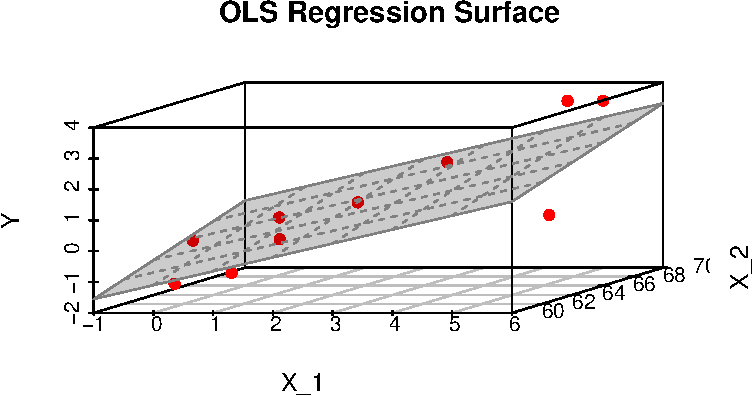
\includegraphics{./04-MultipleReg_files/figure-pdf/unnamed-chunk-1-1.pdf}

}

\end{figure}

\hypertarget{some-quantities-of-interest}{%
\section{Some Quantities of
Interest}\label{some-quantities-of-interest}}

\textbf{Predicted values and residuals.}

\begin{itemize}
\tightlist
\item
  The (OLS) \textbf{predicted values}: \(\hat{Y}_i=X_i'\hat\beta\).\\
  In matrix notation:
  \(\hat Y=X\underbrace{(X'X)^{-1}X'Y}_{\hat\beta}=P_X Y\)
\item
  The (OLS) \textbf{residuals}: \(\hat\varepsilon_i=Y_i-\hat{Y}_i\). In
  matrix notation:
  \(\hat\varepsilon=Y-\hat{Y}=\left(I_n-X(X'X)^{-1}X'\right)Y=M_X Y\)
\end{itemize}

\textbf{Projection matrices.}

The matrix

\[
P_X=X(X'X)^{-1}X'
\]

is the \((n\times n)\) \textbf{projection matrix} that projects any
vector from \(\mathbb{R}^n\) into the column space spanned by the column
vectors of \(X\) and

\[
M_X=I_n-X(X'X)^{-1}X'=I_n-P_X
\]

is the associated \((n\times n)\) \textbf{orthogonal projection matrix}
that projects any vector from \(\mathbb{R}^n\) into the vector space
that is orthogonal to that spanned by \(X\).

The projection matrices \(P_X\) and \(M_X\) have some nice properties:

\begin{enumerate}
\def\labelenumi{(\alph{enumi})}
\tightlist
\item
  \(P_X\) and \(M_X\) are \textbf{symmetric}, i.e.~\(P_X=P_X'\) and
  \(M_X=M_X'\).
\item
  \(P_X\) and \(M_X\) are \textbf{idempotent}, i.e.~\(P_XP_X=P_X\) and
  \(M_X M_X=M_X\).
\item
  Moreover, we have that \(X'P_X=X'\), \(P_XX=X\), \(X'M_X=0\),
  \(M_XX=0\), and \(P_XM_X=0\).
\end{enumerate}

All of these properties follow directly from the definitions of \(P_X\)
and \(M_X\) (check it out). Using these properties one can show that the
residual vector
\(\hat\varepsilon=(\hat\varepsilon_1,\dots,\hat\varepsilon_n)'\) is
orthogonal to each of the column vectors in \(X\), i.e \begin{eqnarray}
X'\hat\varepsilon&=&X'M_XY\quad\text{\small(By Def.~of $M_X$)}\\
\Leftrightarrow X'\hat\varepsilon&=&\underset{(K\times n)}{0}\underset{(n\times 1)}{Y}\quad\text{\small(since $X'M_X=0$)}\\
\Leftrightarrow X'\hat\varepsilon&=&\underset{(K\times 1)}{0}
\end{eqnarray} Note that, in the case with intercept, the result
\(X'\hat\varepsilon=0\) implies that
\(\sum_{i=1}^n\hat\varepsilon_i=0\). Moreover, the equation
\(X'\hat\varepsilon=0\) implies also that the residual vector
\(\hat{\varepsilon}\) is orthogonal to the predicted values vector,
since \begin{align*}
X'\hat\varepsilon&=0\\
\Rightarrow\;\hat\beta'X'\hat\varepsilon&=\hat\beta'0\\
\Leftrightarrow\;\hat Y'\hat\varepsilon&=0.
\end{align*}

Another insight from equation \(X'\hat\varepsilon=0\) is that the vector
\(\hat\varepsilon\) has to satisfy \(K\) linear restrictions which means
it looses \(K\) degrees of freedom.\footnote{Take a look at this
  visualization: \url{https://rpsychologist.com/d3/ci/}} Consequently,
the vector of residuals \(\hat\varepsilon\) has only \(n-K\) so-called
\emph{degrees of freedom}. This loss of \(K\) degrees of freedom also
appears in the definition of the \emph{unbiased} variance estimator
\begin{align}
  s_{UB}^2&=\frac{1}{n-K}\sum_{i=1}^n\hat\varepsilon_i^2\label{EqVarEstim}.
\end{align}

\textbf{Variance decomposition:} A further useful result that can be
shown using the properties of \(P_X\) and \(M_X\) is that
\(Y'Y=\hat{Y}'\hat{Y}+\hat\varepsilon'\hat\varepsilon\), i.e.
\begin{eqnarray*}
Y'Y&=&(\hat Y+\hat\varepsilon)'(\hat Y+\hat\varepsilon)\notag\\
  &=&(P_XY+M_XY)'(P_XY+M_XY)\notag\\
  &=&(Y'P_X'+Y'M_X')(P_XY+M_XY)\notag\\
  &=&Y'P_X'P_XY+Y'M_X'M_XY+0\notag\\
  &=&\hat{Y}'\hat{Y}+\hat\varepsilon'\hat\varepsilon
\end{eqnarray*} The decomposition

\[
\hat{Y}'\hat{Y}+\hat\varepsilon'\hat\varepsilon
\]

is the basis for the well-known variance decomposition result for OLS
regressions.

\leavevmode\vadjust pre{\hypertarget{thm-vardecomp}{}}%
\begin{theorem}[]\label{thm-vardecomp}

For the linear OLS regression model Equation~\ref{eq-LinMod} with
intercept, the total sample variance of the dependent variable
\(Y_1,\dots,Y_n\) can be decomposed as following: \begin{eqnarray}
\underset{\text{total sample variance}}{\frac{1}{n}\sum_{i=1}^n\left(Y_i-\bar{Y}\right)^2}&=&\underset{\text{explained sample variance}}{\frac{1}{n}\sum_{i=1}^n\left(\hat{Y}_i-\bar{\hat{Y}}\right)^2}+\underset{\text{unexplained sample variance}}{\frac{1}{n}\sum_{i=1}^n\hat\varepsilon_i^2,}\label{VarDecomp}
\end{eqnarray} where \(\bar{Y}=\frac{1}{n}\sum_{i=1}^nY_i\) and
\(\bar{\hat{Y}}=\frac{1}{n}\sum_{i=1}^n\hat{Y}_i\).

\end{theorem}

\begin{proof}

From equation \(X'\hat\varepsilon=0\) we have for regressions with
intercept that \(\sum_{i=1}^n\hat\varepsilon_i=0\). Hence, from
\(Y_i=\hat{Y}_i+\hat\varepsilon_i\) it follows that \begin{eqnarray*}
  \frac{1}{n}\sum_{i=1}^n Y_i&=&\frac{1}{n}\sum_{i=1}^n \hat{Y}_i+\frac{1}{n}\sum_{i=1}^n \hat\varepsilon_i\\
  \bar{Y}&=&\bar{\hat{Y}}+0
\end{eqnarray*}

Using the decomposition
\(Y'Y=\hat{Y}'\hat{Y}+\hat\varepsilon'\hat\varepsilon\), we can now
derive the result: \begin{eqnarray*}
   Y'Y&=&\hat{Y}'\hat{Y}+\hat\varepsilon'\hat\varepsilon\\
   Y'Y-n\bar{Y}^2&=&\hat{Y}'\hat{Y}-n\bar{Y}^2+\hat\varepsilon'\hat\varepsilon\\
   Y'Y-n\bar{Y}^2&=&\hat{Y}'\hat{Y}-n\bar{\hat{Y}}^2+\hat\varepsilon'\hat\varepsilon\quad\text{(by $\bar{Y}=\bar{\hat{Y}}$)}\\
   \sum_{i=1}^nY_i^2-n\bar{Y}^2&=&\sum_{i=1}^n\hat{Y}_i^2-n\bar{\hat{Y}}^2+\sum_{i=1}^n\hat\varepsilon_i^2\\
   \sum_{i=1}^n(Y_i-\bar{Y})^2&=&\sum_{i=1}^n(\hat{Y}_i-\bar{\hat{Y}})^2+\sum_{i=1}^n\hat\varepsilon_i^2\quad\square\\
\end{eqnarray*}

\end{proof}

\hypertarget{coefficients-of-determination-r2-and-overliner2}{%
\subsubsection*{\texorpdfstring{Coefficients of determination: \(R^2\)
and
\(\overline{R}^2\)}{Coefficients of determination: R\^{}2 and \textbackslash overline\{R\}\^{}2}}\label{coefficients-of-determination-r2-and-overliner2}}
\addcontentsline{toc}{subsubsection}{Coefficients of determination:
\(R^2\) and \(\overline{R}^2\)}

The larger the proportion of the explained variance, the better is the
fit of the model. This motivates the definition of the so-called \(R^2\)
coefficient of determination: \begin{eqnarray*}
R^2=\frac{\sum_{i=1}^n\left(\hat{Y}_i-\bar{\hat{Y}}\right)^2}{\sum_{i=1}^n\left(Y_i-\bar{Y}\right)^2}\;=\;1-\frac{\sum_{i=1}^n\hat{\varepsilon}_i^2}{\sum_{i=1}^n\left(Y_i-\bar{Y}\right)^2}
\end{eqnarray*} Obviously, we have that \(0\leq R^2\leq 1\). The closer
\(R^2\) lies to \(1\), the better is the fit of the model to the
observed data. However, a high/low \(R^2\) does not mean a
validation/falsification of the estimated model. Any relation (i.e.,
model assumption) needs a plausible explanation from relevant economic
theory. The most often criticized disadvantage of the \(R^2\) is that
additional regressors (relevant or not) will always increase the
\(R^2\). Here is an example of the problem.

\begin{Shaded}
\begin{Highlighting}[]
\FunctionTok{set.seed}\NormalTok{(}\DecValTok{123}\NormalTok{)}
\NormalTok{n     }\OtherTok{\textless{}{-}} \DecValTok{100}               \CommentTok{\# Sample size}
\NormalTok{X     }\OtherTok{\textless{}{-}} \FunctionTok{runif}\NormalTok{(n, }\DecValTok{0}\NormalTok{, }\DecValTok{10}\NormalTok{)   }\CommentTok{\# Relevant X variable}
\NormalTok{X\_ir  }\OtherTok{\textless{}{-}} \FunctionTok{runif}\NormalTok{(n, }\DecValTok{5}\NormalTok{, }\DecValTok{20}\NormalTok{)   }\CommentTok{\# Irrelevant X variable}
\NormalTok{error }\OtherTok{\textless{}{-}} \FunctionTok{rt}\NormalTok{(n, }\AttributeTok{df =} \DecValTok{10}\NormalTok{)}\SpecialCharTok{*}\DecValTok{10}  \CommentTok{\# True error}
\NormalTok{Y     }\OtherTok{\textless{}{-}} \DecValTok{1} \SpecialCharTok{+} \DecValTok{5} \SpecialCharTok{*}\NormalTok{ X }\SpecialCharTok{+}\NormalTok{ error    }\CommentTok{\# Y variable}
\NormalTok{lm1   }\OtherTok{\textless{}{-}} \FunctionTok{summary}\NormalTok{(}\FunctionTok{lm}\NormalTok{(Y}\SpecialCharTok{\textasciitilde{}}\NormalTok{X))     }\CommentTok{\# Correct OLS regression }
\NormalTok{lm2   }\OtherTok{\textless{}{-}} \FunctionTok{summary}\NormalTok{(}\FunctionTok{lm}\NormalTok{(Y}\SpecialCharTok{\textasciitilde{}}\NormalTok{X}\SpecialCharTok{+}\NormalTok{X\_ir))}\CommentTok{\# OLS regression with X\_ir }
\NormalTok{lm1}\SpecialCharTok{$}\NormalTok{r.squared }\SpecialCharTok{\textless{}}\NormalTok{ lm2}\SpecialCharTok{$}\NormalTok{r.squared}
\end{Highlighting}
\end{Shaded}

\begin{verbatim}
[1] TRUE
\end{verbatim}

So, \(R^2\) increases here even though \texttt{X\_ir} is a completely
irrelevant explanatory variable. Because of this, the \(R^2\) cannot be
used as a criterion for model selection. Possible solutions are given by
penalized criterions such as the so-called \textbf{adjusted} \(R^2\),
\(\overline{R}^2,\) defined as \begin{eqnarray*}
  \overline{R}^2&=&1-\frac{\frac{1}{n-K}\sum_{i=1}^n\hat{\varepsilon}^2_i}{\frac{1}{n-1}\sum_{i=1}^n\left(Y_i-\bar{Y}\right)^2}\leq R^2%\\
  %=\dots=
  %&=&1-\frac{n-1}{n-K}\left(1-R^2\right)\quad{\small\text{(since $1-R^2=(\sum_i\hat\varepsilon_i^2)/(\sum_i(Y_i-\bar{Y}))$)}}\\
  %&=&1-\frac{n-1}{n-K}+\frac{n-1}{n-K}R^2\quad+\frac{K-1}{n-K}R^2-\frac{K-1}{n-K}R^2\\
  %&=&1-\frac{n-1}{n-K}+R^2\quad+\frac{K-1}{n-K}R^2\\
  %&=&-\frac{K-1}{n-K}+R^2\quad+\frac{K-1}{n-K}R^2\\
  %&=&R^2-\underbrace{\frac{K-1}{n-K}\left(1-R^2\right)}_{\geq 0\;\text{and}\;\leq(K-1)/(n-K)}\;\leq\;R^2
\end{eqnarray*} The adjustment is in terms of the degrees of freedom
\(n-K\).

\hypertarget{method-of-moments-estimator}{%
\section{Method of Moments
Estimator}\label{method-of-moments-estimator}}

The methods of moments estimator exploits the exogeneity assumption that
\(E(\varepsilon_i|X_i)=0\) for all \(i=1,\dots,n\) (Assumption 2).
Remember that \(E(\varepsilon_i|X_i)=0\) implies that
\(E(X_{ik}\varepsilon_i)=0\) for all \(i=1,\dots,n\) and all
\(k=1,\dots,K\). The fundamental idea behind ``method of moments
estimation'' is to use the sample analogues of the population moment
restrictions \(E(X_{ik}\varepsilon_i)=0\), \(k=1,\dots,K,\) for deriving
the estimator:

\[
\begin{array}{c||c}
\text{$K$ population moment restrictions\quad}&\text{$K$ sample moment restrictions}\\[2ex]
\left.\begin{array}{c}
E(\varepsilon_i)=0\\
E(X_{i2}\varepsilon_i)=0\\
\vdots\\
E(X_{iK}\varepsilon_i)=0
\end{array}
\right\}\Leftrightarrow E(X_i\varepsilon_i)=\underset{(K\times 1)}{0} &
\left.\begin{array}{c}
\displaystyle
\frac{1}{n}\sum_{i=1}^n\hat\varepsilon_i=0\\
\displaystyle
\frac{1}{n}\sum_{i=1}^nX_{i2}\hat\varepsilon_i=0\\
\vdots\\
\displaystyle
\frac{1}{n}\sum_{i=1}^nX_{iK}\hat\varepsilon_i=0\\
\end{array}
\right\}\Leftrightarrow \displaystyle\frac{1}{n}\sum_{i=1}^nX_i\hat\varepsilon_i=\underset{(K\times 1)}{0}
\end{array}
\]

\bookmarksetup{startatroot}

\hypertarget{sec-ssinf}{%
\chapter{Small Sample Inference}\label{sec-ssinf}}

The content of this chapter is very much inspired by the book by Hayashi
(2000).

It's is very hard to say when a sample size \(n\) is small. Often people
say something like \(n<30\) means small samples and \(n\geq 30\) large
samples, but this is, of course, only a very rough rule of thumb that
may fail. The core issue with small sample sizes is that we cannot do
inference using the central limit theorem. Thus we need rather strict
assumptions on the distribution of the error term, in order to do
\textbf{exact} inference in finite samples.

\textbf{Exact inference:} By ``exact inference'' we mean correct
inference for each sample size \(n\). That is, no asymptotic
\((n\to\infty)\) arguments will be used.

\textbf{Assumptions:} Recall that we, in general, did not impose a
complete distributional assumption on \(\varepsilon\) in Assumption 4
(Chapter~\ref{sec-MLR}); the i.i.d. normal case in Assumption 4 was only
one possible \emph{option}. However, to do exact inference, the
normality Assumption on the error terms is not a mere option, but a
\emph{necessity}. So for this chapter we assume that Assumptions 1-3
from Chapter~\ref{sec-MLR} hold and that additionally the following
assumption holds:

\textbf{Assumption 4\(^\boldsymbol{\ast}\): Error distribution:} For
small sample cases, we assume that the error terms are \textbf{i.i.d.
normal}, i.e.,
\(\varepsilon_i\overset{\operatorname{i.i.d.}}{\sim}\mathcal{N}(0,\sigma^2)\)
for all \(i=1,\dots,n\) which leads to spherical errors. That is,

\[
\varepsilon\sim\mathcal{N}\left(0,\sigma^2I_n\right),
\]

where \(\varepsilon=(\varepsilon_1,\dots,\varepsilon_n)'\).

\bigskip

\leavevmode\vadjust pre{\hypertarget{thm-normalbeta}{}}%
\begin{theorem}[]\label{thm-normalbeta}

\bookmarksetup{startatroot}

\hypertarget{normality-of-hatbeta}{%
\chapter{\texorpdfstring{Normality of
\(\hat\beta\)}{Normality of \textbackslash hat\textbackslash beta}}\label{normality-of-hatbeta}}

Under Assumptions 1-4\(^\ast\) we have that

\begin{equation}\protect\hypertarget{eq-ssnorm}{}{
\hat\beta_n|X \sim \mathcal{N}\left(\beta,Var(\hat\beta_n|X)\right),
}\label{eq-ssnorm}\end{equation}

where \(Var(\hat\beta_n|X)=\sigma^2(X'X)^{-1}\).

\end{theorem}

This result follows from noting that
\(\hat\beta_n=(X'X)^{-1}X'Y=\beta+(X'X)^{-1}X'\varepsilon\) and because
\((X'X)^{-1}X'\varepsilon\) is just a linear combination of the normally
distributed error terms \(\varepsilon\) which, therefore, is again
normally distributed, conditionally on \(X\). Note that the specific
normal distribution depends on the observed realization of \(X\).

\textbf{Remark:} The subscript \(n\) in \(\hat\beta_n\) is here only to
emphasize that the distribution of \(\hat\beta_n\) depends on \(n\); we
will, however, often simply write \(\hat\beta\).

\hypertarget{sec-testmultp}{%
\section{Hypothesis Tests about Multiple Parameters
(F-Tests)}\label{sec-testmultp}}

Let us consider the following system of \(q\)-many null hypotheses:
\begin{align*}
H_0: \underset{(q\times K)}{R}\underset{(K\times 1)}{\beta} - \underset{(q\times 1)}{r} = \underset{(q\times 1)}{0},
\end{align*} where the \((q \times K)\) matrix \(R\) and the
\(q\)-vector \(r=(r_{1},\dots,r_{q})'\) are chosen by the statistician
to specify her/his null hypothesis about the unknown true parameter
vector \(\beta\). To make sure that there are no redundant equations, it
is required that \(\operatorname{rank}(R)=q\).

We must also specify the alternative against which we are testing the
null hypothesis, for instance \begin{equation*}
H_A: R\beta -r \neq 0
\end{equation*}

The above multiple parameter hypotheses cover also the special case of
single parameter hypothesis; for instance, by setting
\(R=(0,1,0\dots,0)\) and \(r=0\) one get's \begin{equation*}
\begin{array}{ll}
H_0:  & \beta_{k}=0 \\
H_A:  & \beta_{k} \ne 0 \\
\end{array}
\end{equation*}

Under our assumptions (Assumptions 1 to 4\(^\ast\)), we have that

\[
(R\hat\beta_n-r)|X\sim\mathcal{N}\left(R\beta -r,RVar(\hat\beta_n|X)R'\right).
\]

So, the realizations of \((R\hat\beta_n -r)|X\) will scatter around the
\emph{unknown} \((R\beta -r)\) in a non-systematical, Gaussian fashion.
Therefore, if the null hypothesis is correct (i.e., \((R\beta-r)=0\)),
the realizations of \((R\hat\beta_n-r)|X\) scatter around the
\(q\)-vector \(0\). If, however, the alternative hypothesis is correct
(i.e., \((R\beta-r)=a\neq 0\)), the realizations of \(R\hat\beta_n-r|X\)
scatter around the \(q\)-vector \(a\neq 0\). So, under the alternative
hypothesis, there will be a systematic location-shift of the
\(q\)-dimensional random variable \(R\hat\beta_n|X\) away from \(r\)
which we try to detect using statistical hypothesis testing.

\hypertarget{the-test-statistic-and-its-null-distribution}{%
\subsection{The Test Statistic and its Null
Distribution}\label{the-test-statistic-and-its-null-distribution}}

The fact that \((R\hat\beta_n-r)\in\mathbb{R}^q\) is a \(q\)-dimensional
random variable makes it a little bothersome to use as a test-statistic.
Fortunately, we can turn \((R\hat\beta_n-r)\) into a scalar-valued test
statistic using the following quadratic form:

\[
W=\underbrace{(R\hat\beta_n -r)'}_{(1\times q)}\underbrace{[RVar(\hat\beta_n|X)R']^{-1}}_{(q\times q)}\underbrace{(R\hat\beta_n -r)}_{(q\times 1)}
\]

Note that the test statistic \(W\) is simply measuring the distance
(it's a weighted L2-distance of two vectors) between \(R\hat\beta_n\)
and \(r\).

Under the null hypothesis (i.e., if the null hypothesis is true), \(W\)
is just a sum of \(q\)-many independent squared standard normal random
variables. Therefore, under the null hypothesis, \(W\) is chi-square
distributed with \(q\) degrees of freedom (see
Section~\ref{sec-chisqdist}),

\[
W\overset{H_0}{\sim} \chi^2_{(q)}.
\]

Note that the distribution of \(W\) conditional on \(X\) does not depend
on \(X\); i.e.~\(W|X\overset{H_0}{\sim}\chi^2_{(q)}\), but
\(\chi^2_{(q)}\) does not depend on \(X\), thus we can write
\(W\overset{H_0}{\sim} \chi^2_{(q)}.\)

Usually, we do not know \(Var(\hat\beta_n|X)\) , but need to estimate
this quantity from the data. Unfortunately, in the small sample case, we
can only deal with homoskedastic error terms. For truly exact finite
sample inference, we need a variance estimator for which we can derive
the exact small sample distribution. Therefore, we assume in Assumption
4\(^*\) spherical errors (i.e., \(Var(\varepsilon|X)=I_n\sigma^2\))
which yields that \(Var(\hat\beta_n|X)=\sigma^2(X'X)^{-1}\), and where
\(\sigma^2\) can be estimated by the unbiased (\(UB\)) variance
estimator

\[
s_{UB}^2=(n-K)^{-1}\sum_{i=1}^n\hat\varepsilon_i^2.
\]

From the normality assumption in Assumption 4\(^*\), it follows then
that

\begin{equation}\protect\hypertarget{eq-distsquared}{}{
\frac{(n-K)}{\sigma^{2}}s_{UB}^2\sim\chi^2_{(n-K)}.
}\label{eq-distsquared}\end{equation}

The \(F\) test statistic

\[
F=(R\hat\beta_n -r)'[R(s_{UB}^2(X'X)^{-1})R']^{-1}(R\hat\beta_n -r)/q
\]

takes into account the additional randomness due to the estimator
\(s_{UB}^2\), which leads to the following exact null distribution of
the \(F\) test

\begin{equation}\protect\hypertarget{eq-Ftest}{}{
F\overset{H_0}{\sim} F_{(q,n-K)},
}\label{eq-Ftest}\end{equation}

where \(F_{(q,n-K)}\) denotes the \(F\)-distribution with \(q\)
numerator and \(n-K\) denominator degrees of freedom. As in the case of
\(W\), the distribution of \(F\) conditional on \(X\) does not depend on
\(X\); i.e.~\(F|X\overset{H_0}{\sim}F_{(q,n-K)}\), but \(F_{(q,n-K)}\)
does not depend on \(X\), thus we can write
\(F\overset{H_0}{\sim}F_{(q,n-K)}.\)

The distributional statements in Equation~\ref{eq-distsquared} and
Equation~\ref{eq-Ftest} are a little cumbersome to derive and we do not
go into details here, but in case you're interested you can find some
more details in Chapter 1 of Hayashi (2000).

By contrast to \(W\), \(F\) is now a practically useful test statistic,
and we can use the observed value \(F_{\text{obs}}\) to measure the
distance of our estimate \(R\hat\beta_n\) from value \(r\). Observed
values, \(F_{\text{obs}}\), that are ``unusually large'' under the null
hypothesis, lead to a rejection of the null hypothesis. The null
distribution \(F_{(q,n-K)}\) of \(F\) is used to judge what's
``unusually large'' under the null hypothesis.

\textbf{The F distribution:} The F distribution is a ratio of two
\(\chi^2\) distributions. It has two parameters: the numerator degrees
of freedom, and the denominator degrees of freedom. Each combination of
the parameters yields a different F distribution. See
Section~\ref{sec-Fdist} for more information on the \(F\) distribution.

\begin{figure}

{\centering 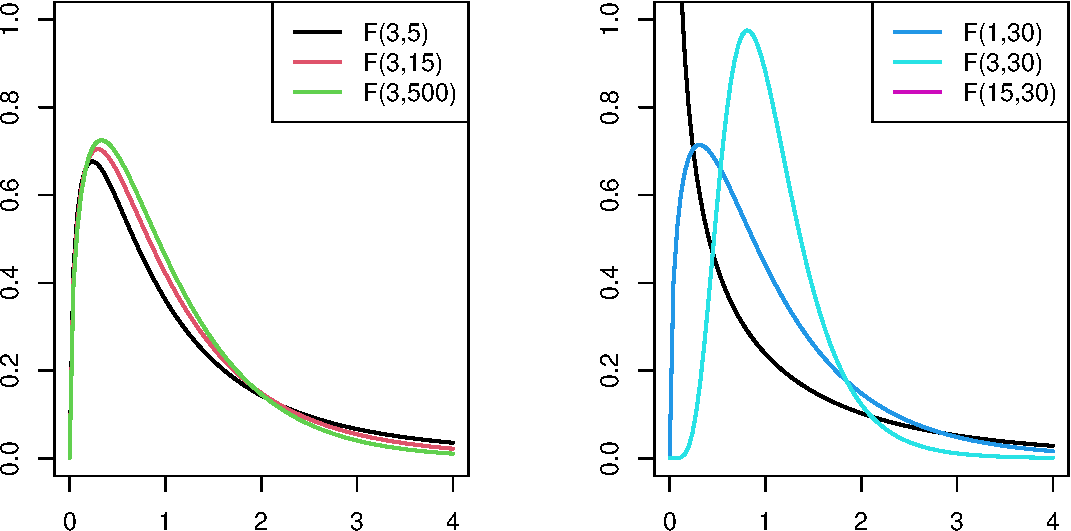
\includegraphics{./05-Small-Sample-Inference_files/figure-pdf/unnamed-chunk-1-1.pdf}

}

\end{figure}

\hypertarget{ch:testingsinglep}{%
\section{Tests about One Parameter (t-Tests)}\label{ch:testingsinglep}}

For testing a hypothesis about only one parameter \(\beta_k\), with
\(k=1,\dots,K\) \begin{equation*}
\begin{array}{ll}
H_0: & \beta_k=r\\
H_A: & \beta_k\ne r\\
\end{array}
\end{equation*} the \((q\times K)=(1\times K)\)-matrix \(R\) equals a
row-vector of zeros but with a one as the \(k\)th element; e.g., for
\(k=2\) we have \(R=(0,1,0,\dots,0).\) Thus, the \(F\) test statistic
simplifies to

\[
F=\frac{\left(\hat{\beta}_k-r\right)^2}{\widehat{Var}(\hat{\beta}_k|X)},
\]

where \(\widehat{Var}(\hat{\beta}_k|X)=s^2_{UB}[(X'X)^{-1}]_{kk}.\)

Taking square roots yields the \(t\) test statistic

\[
t=\frac{\hat{\beta}_k-r}{\widehat{\operatorname{SE}}(\hat{\beta}_k|X)},
\]

where
\(\widehat{\operatorname{SE}}(\hat{\beta}_k|X)=s_{UB}[(X'X)^{-1/2}]_{kk}.\)

Under the null hypothesis, the \(t\) test statistic is \(t\)-distributed
with \(n-K\) degrees of freedom

\[
t\overset{H_0}{\sim}t_{(n-K)}.
\]

Thus the \(t\)-distribution with \(n-K\) degrees of freedom is the
appropriate distribution to judge whether or not an observed value
\(t_{obs}\) of the test statistic is unusually small or large under the
null hypothesis.

\textbf{Note:} All commonly used statistical software packages report
\(t\)-tests testing the null hypothesis \(H_0:\beta_k=0\), i.e., with
\(r=0\). This means to test the null hypothesis that \(X_k\) has ``no
(linear) effect'' on \(Y\).

The following plot illustrates that as the degrees of freedom increase,
the shape of the \(t\) distribution comes closer to that of a standard
normal bell curve. Already for \(25\) degrees of freedom we find little
difference to the standard normal density. In case of small degrees of
freedom values, we find the distribution to have heavier tails than a
standard normal.

\begin{figure}

{\centering 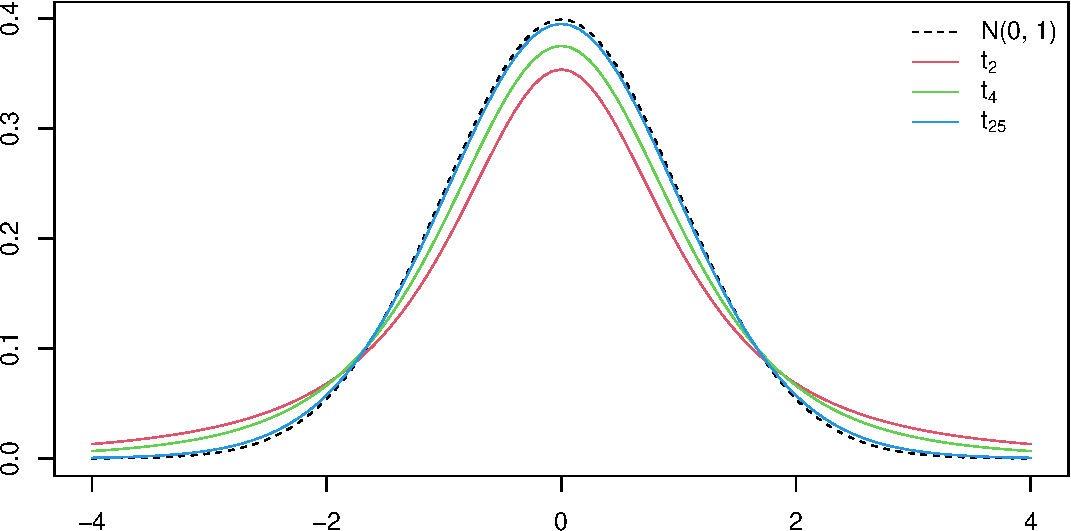
\includegraphics{./05-Small-Sample-Inference_files/figure-pdf/unnamed-chunk-2-1.pdf}

}

\end{figure}

\hypertarget{testtheory}{%
\section{Testtheory}\label{testtheory}}

\hypertarget{significance-level-alpha}{%
\subsection{\texorpdfstring{Significance Level
\(\alpha\)}{Significance Level \textbackslash alpha}}\label{significance-level-alpha}}

To actually test the null hypothesis (e.g., \(H_0\): \(R\beta-r=0\) or
\(H_0\): \(\beta_k=0\)), we need to have a decision rule on when we will
reject or not reject the null hypothesis. This amounts to deciding on a
probability with which we are comfortable with committing a Type I error
(\(\alpha\)-error): rejecting the null hypothesis when it is in fact
true. The probability of such a Type I error shall be bounded from above
by a (small) significance level \(\alpha\), that is

\[
P(\text{reject } H_0| H_0\text{ is true})=P(\text{Type I Error})=\alpha
\]

For a given significance level (e.g., \(\alpha=0.05\)) and a given
alternative hypothesis, we can divide the range of all possible values
of the test statistic (i.e., \(\mathbb{R}\) since both
\(t\in\mathbb{R}\) and \(F\in\mathbb{R}\)) into a \textbf{rejection
region} and a \textbf{non-rejection region} by using \textbf{critical
values} derived from the distribution of the test statistic under the
null hypothesis. We can do this because the test statistics \(t\) and
\(F\) have known distributions under the null hypothesis
(\(t\overset{H_0}{\sim}t_{n-K}\) and
\(F\overset{H_0}{\sim}F_{(q,n-K)}\)).

Indeed, under Assumption 4\(^\ast\), we know the \emph{exact} null
distributions for every sample size \(n\). Having decided on the
rejection and non-rejection regions, we only need to check whether the
observed (obs) sample values \(t_{obs}\) or \(F_{obs}\) of the test
statistics \(t\) or \(F\) are either in the rejection or in the
non-rejection region to either rejection the null hypothesis or not to
rejection the null hypothesis.

\textbf{Non-conservative versus conservative tests:} Since the test
statistics \(F\) and \(t\) are continuous random variables of which we
know the \emph{exact} distributions (under Assumptions 1-4\(^\ast\)), we
can find critical values such that

\[
P(\text{Type I Error})=\alpha
\]

We call such tests ``non-conservative'' since the probability of a type
I error equals the significance level \(\alpha\). Test statistics with

\[
P(\text{Type I Error})<\alpha
\]

are called \emph{conservative} test statistics; they lead to valid
inferences, but will detect a correct violation of the null hypothesis
less often than a non-conservative test. A test statistic with
\(P(\text{Type I Error})>\alpha\) leads to \emph{invalid} inferences!

\hypertarget{critical-values}{%
\subsection{Critical Values}\label{critical-values}}

\hypertarget{the-f-test}{%
\subsubsection*{\texorpdfstring{The
\(F\)-Test}{The F-Test}}\label{the-f-test}}
\addcontentsline{toc}{subsubsection}{The \(F\)-Test}

The critical value \(c_{1-\alpha}>0\) defines the

\begin{itemize}
\tightlist
\item
  rejection region, \(]c_{1-\alpha},\infty[\), and
\item
  non-rejection region, \(]0,c_{1-\alpha}]\)
\end{itemize}

which together divide the range of test-statistic values (here
\(\mathbb{R}^+\) since \(F\in\mathbb{R}^+\)) for a given significance
level \(\alpha\in(0,1)\), such that

\[
P(\text{Type I Error})=P_{H_0}\Big(F\in]c_{1-\alpha},\infty[\Big)=\alpha,
\]

where \(c_{1-\alpha}\) is here the \((1-\alpha)\) quantile of the
\(F\)-distribution with \((q,n-K)\) degrees of freedom, and where
\(P_{H_0}\) means that we compute the probability under the assumption
that \(H_0\) is true.

\begin{figure}

{\centering 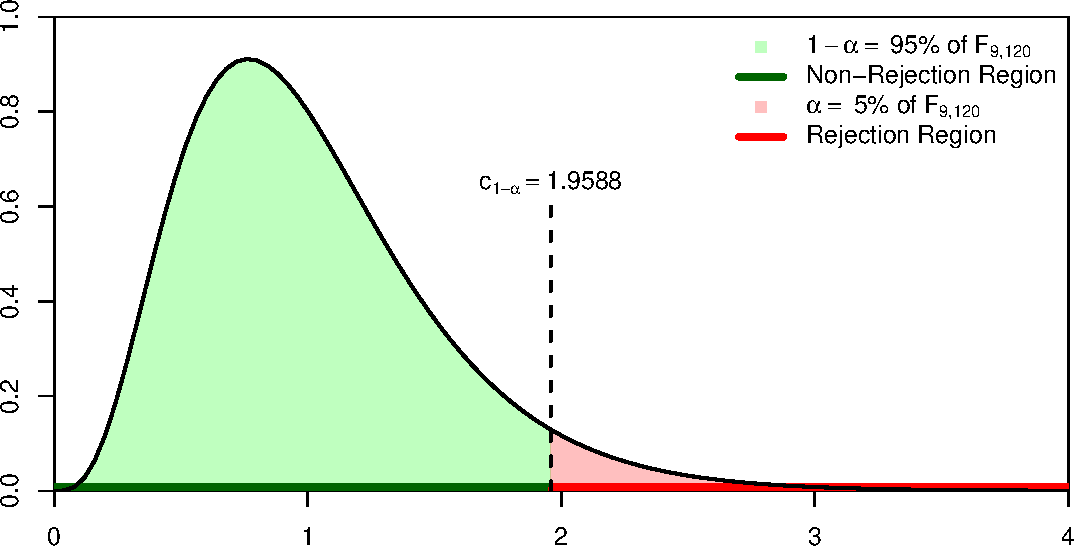
\includegraphics{./05-Small-Sample-Inference_files/figure-pdf/unnamed-chunk-3-1.pdf}

}

\end{figure}

\textbf{The rejection region:} The rejection region describes a range of
values of the test statistic \(F\) which we rarely see if the null
hypothesis is true (only in at most \(\alpha \cdot 100\%\) cases). If
the observed value of the test statistic, \(F_{\text{obs}}\), falls in
this region, we will reject the null hypothesis and accept Type I error
rate of \(\alpha\).

\textbf{The non-rejection region:} The non-rejection region describes a
range of values of the test statistic \(F\) which we expect to see (in
\((1-\alpha) \cdot 100\%\) cases) if the null hypothesis is true. If the
observed value of the test statistic, \(F_{\text{obs}}\) falls in this
region, we will not reject the null hypothesis.

\textbf{Caution:} Not rejecting the null hypothesis does not mean that
we can conclude that the null hypothesis is true. We only had no
sufficiently strong evidence against the null hypothesis. A violation of
the null hypothesis, for instance \(R\beta -r=a\neq 0\), may simply be
too small (too small \(a\) value) to stand out from the estimation
errors (measured by the standard error) in \(\hat\beta_k.\)

Fortunately, you do not need to read old-school distribution tables to
find the critical value \(c_{1-\alpha}\), but can simply use \texttt{R}

\begin{Shaded}
\begin{Highlighting}[]
\NormalTok{df1   }\OtherTok{\textless{}{-}} \DecValTok{9}    \CommentTok{\# numerator df}
\NormalTok{df2   }\OtherTok{\textless{}{-}} \DecValTok{120}  \CommentTok{\# denominator df}
\NormalTok{alpha }\OtherTok{\textless{}{-}} \FloatTok{0.05} \CommentTok{\# significance level}
\DocumentationTok{\#\# Critical value:}
\NormalTok{crit\_value }\OtherTok{\textless{}{-}} \FunctionTok{qf}\NormalTok{(}\AttributeTok{p =} \DecValTok{1}\SpecialCharTok{{-}}\NormalTok{alpha, }\AttributeTok{df1 =}\NormalTok{ df1, }\AttributeTok{df2 =}\NormalTok{ df2)}
\NormalTok{crit\_value}
\end{Highlighting}
\end{Shaded}

\begin{verbatim}
[1] 1.958763
\end{verbatim}

\noindent Changing the significance level from \(\alpha=0.05\) to
\(\alpha=0.01\) makes the critical value \(c_{1-\alpha}\) larger and,
therefore, the rejection region smaller (fewer Type I errors)

\begin{Shaded}
\begin{Highlighting}[]
\NormalTok{alpha }\OtherTok{\textless{}{-}} \FloatTok{0.01}
\DocumentationTok{\#\# Critical value:}
\NormalTok{crit\_value }\OtherTok{\textless{}{-}} \FunctionTok{qf}\NormalTok{(}\AttributeTok{p =} \DecValTok{1}\SpecialCharTok{{-}}\NormalTok{alpha, }\AttributeTok{df1 =}\NormalTok{ df1, }\AttributeTok{df2 =}\NormalTok{ df2)}
\NormalTok{crit\_value}
\end{Highlighting}
\end{Shaded}

\begin{verbatim}
[1] 2.558574
\end{verbatim}

\hypertarget{the-t-test}{%
\subsubsection*{\texorpdfstring{The
\(t\)-Test}{The t-Test}}\label{the-t-test}}
\addcontentsline{toc}{subsubsection}{The \(t\)-Test}

In case of the \(t\)-test, we need to differentiate between two-sided
and one-sided testing.

\hypertarget{two-sided-t-test}{%
\paragraph*{\texorpdfstring{Two-Sided
\(t\)-Test}{Two-Sided t-Test}}\label{two-sided-t-test}}
\addcontentsline{toc}{paragraph}{Two-Sided \(t\)-Test}

Two-sided hypothesis: \begin{equation*}
\begin{array}{ll}
H_0: & \beta_k=r \\
H_A: & \beta_k\ne r
\end{array}
\end{equation*} In case of a two-sided \(t\)-test, we reject the null
hypothesis if the observed realization of the \(t\)-test, \(t_{obs}\),
is ``far away'' from zero either by being sufficiently smaller or
greater than \(r\). The corresponding two-sided critical values are
denoted by \(-c_{1-\alpha/2}=c_{\alpha/2}<0\) and \(c_{1-\alpha/2}>0\),
where \(c_{1-\alpha/2}>0\) is the \((1-\alpha/2)\) quantile of the
\(t\)-distribution with \((n-K)\) degrees of freedom, and where
\(-c_{1-\alpha/2}=c_{\alpha/2}\) due to the symmetry of the
\(t\)-distribution. These critical values defines the following
rejection and the non-rejection regions \begin{align*}
\text{rejection region:}&\hspace{1cm}]-\infty,c_{\alpha/2}[\;\;\cup\;\;]c_{1-\alpha/2}, \infty[\\
\text{non-rejection region:}&\hspace{1cm}[c_{\alpha/2},c_{1-\alpha/2}].
\end{align*} For this rejection region it holds true that

\[
P(\text{Type I Error})=P_{H_0}\Big(t\in\;]-\infty,c_{\alpha/2}[\;\;\cup\;\;]c_{1-\alpha/2}, \infty[\Big)=\alpha.
\]

\begin{figure}

{\centering 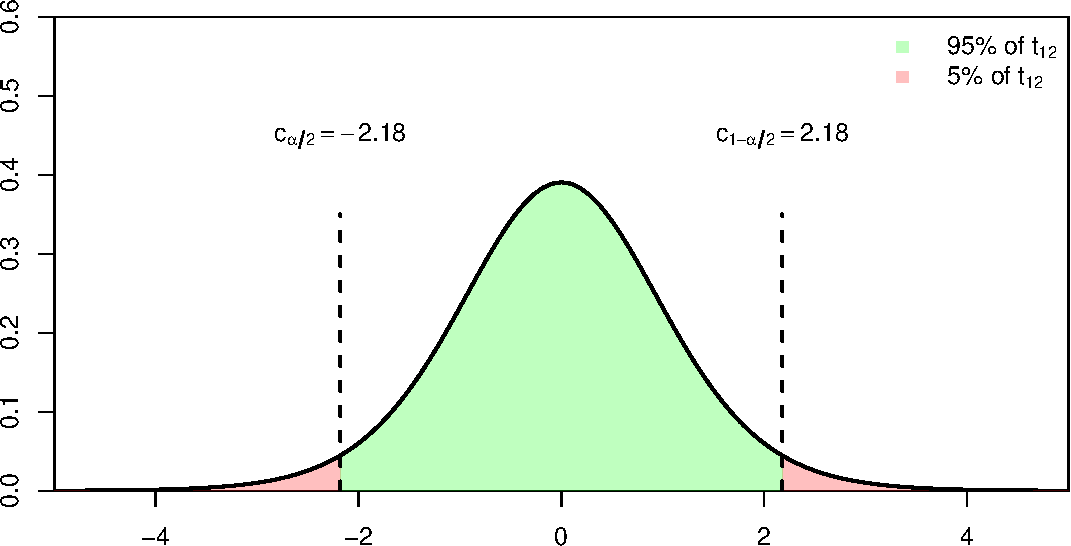
\includegraphics{./05-Small-Sample-Inference_files/figure-pdf/unnamed-chunk-6-1.pdf}

}

\end{figure}

\hypertarget{one-sided-t-test}{%
\paragraph*{\texorpdfstring{One-Sided
\(t\)-Test}{One-Sided t-Test}}\label{one-sided-t-test}}
\addcontentsline{toc}{paragraph}{One-Sided \(t\)-Test}

One-sided hypothesis: \begin{equation*}
\begin{array}{lll}
&H_0: & \beta_k =r\\
&H_A: & \beta_k >r\\
(\text{or}&H_A: & \beta_k< r)
\end{array}
\end{equation*} In case of a one-sided \(t\)-test, we will reject the
null if \(t_{obs}\) is sufficiently ``far away'' from zero in the
relevant direction of \(H_A\). The corresponding critical value is
either \(-c_{1-\alpha}\) (\(H_A:\beta_k< r\)) or \(c_{1-\alpha}\)
(\(H_A:\beta_k> r\)), where \(c_{1-\alpha}\) is the \((1-\alpha)\)
quantile of the \(t\)-distribution with \((n-K)\) degrees of freedom,
and where \(-c_{1-\alpha}=c_{\alpha}\) due to the symmetry of the
\(t\)-distribution. The critical value \(c_{1-\alpha}\) defines the
following rejection and the non-rejection regions:

For \(H_0: \beta_k=0\) \quad versus\quad \(H_A: \beta_k < 0\):
\begin{align*}
\text{rejection region:}   &\hspace{2cm}]-\infty,c_{\alpha}[ \\
\text{non-rejection region:}&\hspace{2cm}[c_{\alpha},\infty[
\end{align*} such that

\[
P(\text{Type I Error})=P_{H_0}\Big(t\in\;]-\infty,c_{\alpha}[\Big)=\alpha.
\]

For \(H_0: \beta_k=0\)\quad versus\quad\(H_A: \beta_k > 0\):
\begin{align*}
\text{rejection region:}&\hspace{1cm}]c_{1-\alpha}, \infty[\\
\text{non-rejection region:}&\hspace{1cm}]-\infty,c_{1-\alpha}]
\end{align*} such that

\[
P(\text{Type I Error})=P_{H_0}\Big(t\in\;]c_{1-\alpha}, \infty[\Big)=\alpha.
\]

\begin{figure}

{\centering 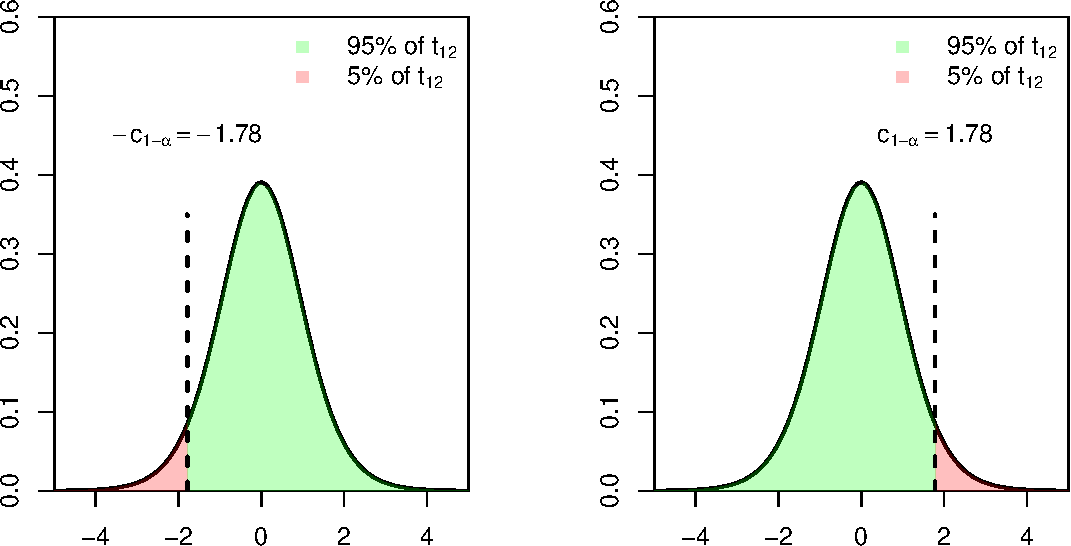
\includegraphics{./05-Small-Sample-Inference_files/figure-pdf/unnamed-chunk-7-1.pdf}

}

\end{figure}

Fortunately, you do not need to read old-school distribution tables to
find the critical values, but you can simply use \texttt{R}

\begin{Shaded}
\begin{Highlighting}[]
\NormalTok{df    }\OtherTok{\textless{}{-}} \DecValTok{16}   \CommentTok{\# degrees of freedom }
\NormalTok{alpha }\OtherTok{\textless{}{-}} \FloatTok{0.05} \CommentTok{\# significance level}
\DocumentationTok{\#\# One{-}sided critical value (= (1{-}alpha) quantile):}
\NormalTok{c\_oneSided }\OtherTok{\textless{}{-}} \FunctionTok{qt}\NormalTok{(}\AttributeTok{p =} \DecValTok{1}\SpecialCharTok{{-}}\NormalTok{alpha, }\AttributeTok{df =}\NormalTok{ df)}
\NormalTok{c\_oneSided}
\end{Highlighting}
\end{Shaded}

\begin{verbatim}
[1] 1.745884
\end{verbatim}

\begin{Shaded}
\begin{Highlighting}[]
\DocumentationTok{\#\# Two{-}sided critical value (= (1{-}alpha/2) quantile):}
\NormalTok{c\_twoSided }\OtherTok{\textless{}{-}} \FunctionTok{qt}\NormalTok{(}\AttributeTok{p =} \DecValTok{1}\SpecialCharTok{{-}}\NormalTok{alpha}\SpecialCharTok{/}\DecValTok{2}\NormalTok{, }\AttributeTok{df =}\NormalTok{ df)}
\DocumentationTok{\#\# lower critical value}
\SpecialCharTok{{-}}\NormalTok{c\_twoSided}
\end{Highlighting}
\end{Shaded}

\begin{verbatim}
[1] -2.119905
\end{verbatim}

\begin{Shaded}
\begin{Highlighting}[]
\DocumentationTok{\#\# upper critical value}
\NormalTok{c\_twoSided}
\end{Highlighting}
\end{Shaded}

\begin{verbatim}
[1] 2.119905
\end{verbatim}

\hypertarget{type-ii-error-and-power}{%
\subsection{Type II Error and Power}\label{type-ii-error-and-power}}

A Type II error is the mistake of not rejecting the null hypothesis when
in fact it should have been rejected. The probability of making a Type
II error equals one minus the probability of correctly rejecting the
null hypothesis (``Power''). For instance, in the case of using the
\(t\)-test to test the null hypothesis \(H_0: \beta_k=0\) versus the
one-sided alternative hypothesis \(H_A:\beta_k>0\)) we have that
\begin{align*}
P(\text{Type II Error})
&=P_{H_A}\Big(t\;\in\;\overbrace{]-\infty,c_{1-\alpha}]}^{\text{non-rejection region}}\Big)\\
&=1-\underbrace{P_{H_A}\Big(t\;\in\;\overbrace{]c_{1-\alpha},\infty[}^{\text{rejection region}}\Big)}_{\text{"Power"}},
\end{align*} where \(P_{H_A}\) means that we compute the probability
under the assumption that \(H_A\) is true.

There is a trade off between the probability of making a Type I error
and the probability of making a Type II error: a lower significance
level \(\alpha\), decreases \(P(\text{Type I Error})\), but necessarily
increases \(P(\text{Type II Error})\) and vice versa. Ideally, we would
have some sense of the costs of making each of these errors, and would
choose our significance level to minimize these total costs. However,
the costs are often difficult to know. Moreover, the probability of
making a Type II error is usually impossible to compute, since we
usually do not know the true distribution of \(\hat\beta_k\) under the
alternative.

For illustration purposes, consider the case of a \(t\) test for a
one-sided hypothesis \begin{equation*}
\begin{array}{ll}
H_0:  & \beta_k=0 \\
H_A:  & \beta_k>0,
\end{array}
\end{equation*} where the true (usually unknown) parameter value is
\(\beta_k=3\) and where the true (usually also unknown) standard error
is
\(\operatorname{SE}(\hat\beta_k|X)=\sqrt{\sigma^2[(X'X)^{-1}]_{kk}}=1.5\).
Only with the knowledge about these usually unknown quantities, we can
derive the distribution of the \(t\)-test statistic under the
alternative hypothesis. The distribution of the \(t\)-test statistic
becomes here a standard normal distribution, since we assume
\(\operatorname{SE}(\hat\beta_k|X)=\sqrt{\sigma^2[(X'X)^{-1}]_{kk}}=1.5\)
to be a known \textbf{deterministic} quantity. (This completely
unrealistic assumption is only used for illustrative purposes; namely to
explain the probability of making a Type II error and the power
(i.e.~\(1-P(\text{Type II Error})\)).)

Under this setup, the distribution under the null hypothesis (i.e., if
\(\beta_k=0\) were true) is:

\[
t=\frac{\hat\beta_k-0}{\sqrt{\sigma^2[(X'X)^{-1}]_{kk}}}\overset{H_0}{\sim}\mathcal{N}(0,1)
\]

Likewise, the distribution under the alternative hypothesis (i.e., for
the actual \(\beta_k=3\)) is: \begin{align*}
t=\frac{\hat\beta_k-0}{\sqrt{\sigma^2[(X'X)^{-1}]_{kk}}}
&=\frac{\hat\beta_k+3-3-0}{\sqrt{\sigma^2[(X'X)^{-1}]_{kk}}}\\[2ex]
\Rightarrow\quad&\underbrace{\frac{\hat\beta_k-3}{\sqrt{\sigma^2[(X'X)^{-1}]_{kk}}}}_{\sim \mathcal{N}(0,1)}+\underbrace{\frac{3-0}{\sqrt{\sigma^2[(X'X)^{-1}]_{kk}}}}_{=\Delta\text{ (mean-shift)}}\overset{H_A}{\sim}\mathcal{N}(\Delta,1)
\end{align*}

So, the mean-shift \(\Delta\) depends on the value of
\(\sqrt{\sigma^2[(X'X)^{-1}]_{kk}}\) (here \(1.5\)) and the difference
between the actual parameter value (\(\beta_k=3\)) and the hypothetical
parameter value under the null-hypothesis (here \(0\)). The following
Graphic illustrates the probability of a type II error and the power for
the case where \(\sqrt{\sigma^2[(X'X)^{-1}]_{kk}}=1.5\) such that
\(\Delta=3/1.5=2\).

\begin{figure}

{\centering 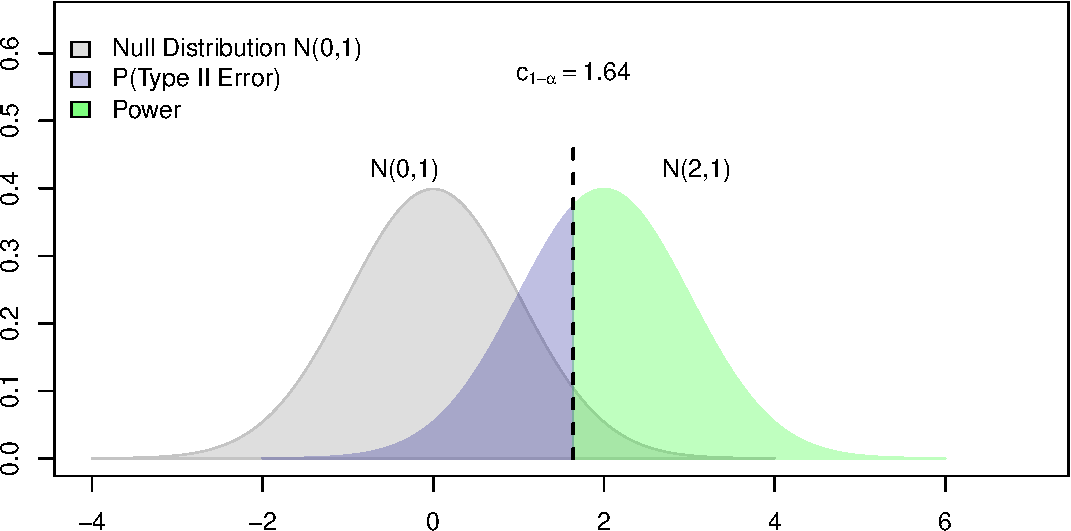
\includegraphics{./05-Small-Sample-Inference_files/figure-pdf/unnamed-chunk-9-1.pdf}

}

\end{figure}

\hypertarget{p-value}{%
\subsection{\texorpdfstring{\(p\)-Value}{p-Value}}\label{p-value}}

The \(p\)-value of a test statistic is the significance level we would
obtain if we took the sample value of the observed test statistic,
\(F_{\text{obs}}\) or \(t_{\text{obs}},\) as the border between the
rejection and non-rejection regions.

\begin{itemize}
\tightlist
\item
  \textbf{\(F\)-test:} \(p=P_{H_0}(F\geq F_{\text{obs}})\)
\item
  \textbf{\(t\)-test:} (\(H_A:\beta_k\neq r\)){]}
  \(p=2\cdot\min\{P_{H_0}(t\leq t_{\text{obs}}),P_{H_0}(t\geq t_{\text{obs}})\}\)
\item
  \textbf{\(t\)-test:} (\(H_A:\beta_k> r\)){]}
  \(p=P_{H_0}(t\geq t_{\text{obs}})\)
\item
  \textbf{\(t\)-test:} (\(H_A:\beta_k< r\)){]}
  \(p=P_{H_0}(t\leq t_{\text{obs}})\)
\end{itemize}

Put another way, the \(p\)-value is the greatest significance level for
which we just fail to reject the null. Therefore, the \(p\)-value is
sometimes also called the marginal significance value.

If the \(p\)-value is strictly smaller than the chosen significance
level \(\alpha\), we reject the null hypothesis.

\hypertarget{sec-CIsmallsample}{%
\section{Confidence Intervals}\label{sec-CIsmallsample}}

We define a two-sided \((1-\alpha)\cdot 100\%\) percent confidence
interval for the \emph{deterministic} (unknown) true \(\beta_k\) as the
\textbf{random interval} \(\operatorname{CI}_{1-\alpha}\) for which

\[
P\Big(\beta_k\in\operatorname{CI}_{1-\alpha}\Big)\geq 1-\alpha.
\]

Derivation of the random interval \(\operatorname{CI}_{1-\alpha}\):

Observe that

\[
\frac{\hat\beta_k-\beta_k}{\widehat{\operatorname{SE}}(\hat\beta_k|X)}\sim t_{(n-K)}
\]

Therefore, \begin{align*}
P\left(-t_{1-\alpha/2,n-K}\leq\frac{\hat\beta_k-\beta_k}{\widehat{\operatorname{SE}}(\hat\beta_k|X)}\leq t_{1-\alpha/2,n-K}\right)=1-\alpha,
\end{align*} where \(t_{1-\alpha/2,n-K}\) denotes the \((1-\alpha)\)
quantile of the \(t\)-distribution with \(n-K\) degrees of freedom.
Next, we can do the following equivalent transformations \begin{align*}
P\left(-t_{1-\alpha/2,n-K}\leq\frac{\hat\beta_k-\beta_k}{\widehat{\operatorname{SE}}(\hat\beta_k|X)}\leq t_{1-\alpha/2,n-K}\right)&=1-\alpha\\
\Leftrightarrow P\left(\hat\beta_k-t_{1-\alpha/2,n-K}\widehat{\operatorname{SE}}(\hat\beta_k|X)\leq \beta_k\leq\hat\beta_k +t_{1-\alpha/2,n-K}\widehat{\operatorname{SE}}(\hat\beta_k|X)\right)&=1-\alpha\\
\Leftrightarrow P\left(\beta_k\in\underbrace{\left[\hat\beta_k-t_{1-\alpha/2,n-K}\widehat{\operatorname{SE}}(\hat\beta_k|X),\;\hat\beta_k +t_{1-\alpha/2,n-K}\widehat{\operatorname{SE}}(\hat\beta_k|X)\right]}_{=:\operatorname{CI}_{1-\alpha}}\right)&=1-\alpha
\end{align*} That is, the random interval

\[
\operatorname{CI}_{1-\alpha}=\left[\hat\beta_k-t_{1-\alpha/2,n-K}\widehat{\operatorname{SE}}(\hat\beta_k|X),\;\hat\beta_k +t_{1-\alpha/2,n-K}\widehat{\operatorname{SE}}(\hat\beta_k|X)\right]
\]

is our \((1-\alpha)\cdot 100\%\) percent confidence interval for
\(\beta_k\).

\textbf{Interpretation:} The random interval
\(\operatorname{CI}_{1-\alpha}\) for \(\beta_k\) contains the true
parameter value \(\beta_k\) in \((1-\alpha)\cdot 100\%\) cases of its
realizations when considering infinitely many realizations.\footnote{Take
  a look at this visualization: \url{https://rpsychologist.com/d3/ci/}}
Unfortunately, this interpretation is not a statement about a single
\(\operatorname{CI}_{1-\alpha}\) computed for given data. A given,
realized \(\operatorname{CI}_{1-\alpha}\) will either contain the true
parameter \(\beta_k\) or not, and usually we do not know the answer. So,
the problem with \(\operatorname{CI}\)s is that they are quite hard to
interpret. However, they are very well suited for a visual comparison of
the estimation uncertainties in different parameter estimators, for
instance, across \(\hat\beta_k\), \(k=1,\dots,K\).

\begin{figure}

{\centering 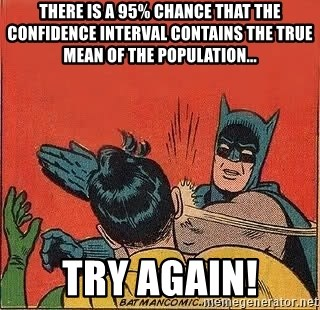
\includegraphics{./images/Meme_CI.jpg}

}

\caption{Try again!}

\end{figure}

\hypertarget{sec-PSSI}{%
\section{Practice: Small Sample Inference}\label{sec-PSSI}}

Let's apply the above exact inference methods using \texttt{R}. First,
we program a function \texttt{myDataGenerator()} which allows us to
generate data from the following model, i.e., from the following fully
specified data generating process: \begin{align*}
Y_i &=\beta_1+\beta_2X_{i2}+\beta_3X_{i3}+\varepsilon_i,\qquad i=1,\dots,n\\
\beta &=(\beta_1,\beta_2,\beta_3)'=(2,3,4)'\\
X_{i2}&\sim U[2,10]\\
X_{i3}&\sim U[12,22]\\
\varepsilon_i&\sim\mathcal{N}(0,3^2),
\end{align*} where \((Y_i,X_i)\) is assumed i.i.d. across
\(i=1,\dots,n\). Below, in the codes, I use \(n=10\), but, of course,
other sample sizes can be considered too. Under the assumptions of this
chapter, we do exact inference that is specific to any given sample size
\(n\).

The below function \texttt{myDataGenerator()} allows to sample new
realizations of \(Y_1,\dots,Y_n\) conditionally on a given data matrix
\(X\). Moreover, you can provide your own values for the sample size
\(n\) and for the parameter vector \(\beta=(\beta_1,\beta_2,\beta_3)'\).

\begin{Shaded}
\begin{Highlighting}[]
\DocumentationTok{\#\# Function to generate artificial data}
\DocumentationTok{\#\# If X=NULL: new X variables are generated}
\DocumentationTok{\#\# If the user gives X variables, }
\DocumentationTok{\#\# the sampling of new Y variables is conditionally on }
\DocumentationTok{\#\# the given X variables.}
\NormalTok{myDataGenerator }\OtherTok{\textless{}{-}} \ControlFlowTok{function}\NormalTok{(n, beta, }\AttributeTok{X=}\ConstantTok{NULL}\NormalTok{, }\AttributeTok{sigma=}\DecValTok{3}\NormalTok{)\{}
  \ControlFlowTok{if}\NormalTok{(}\FunctionTok{is.null}\NormalTok{(X))\{}
\NormalTok{    X   }\OtherTok{\textless{}{-}} \FunctionTok{cbind}\NormalTok{(}\FunctionTok{rep}\NormalTok{(}\DecValTok{1}\NormalTok{, n), }
                 \FunctionTok{runif}\NormalTok{(n, }\DecValTok{2}\NormalTok{, }\DecValTok{10}\NormalTok{), }
                 \FunctionTok{runif}\NormalTok{(n,}\DecValTok{12}\NormalTok{, }\DecValTok{22}\NormalTok{))}
\NormalTok{  \}}
\NormalTok{  eps  }\OtherTok{\textless{}{-}} \FunctionTok{rnorm}\NormalTok{(n, }\AttributeTok{sd=}\NormalTok{sigma)}
\NormalTok{  Y    }\OtherTok{\textless{}{-}}\NormalTok{ X }\SpecialCharTok{\%*\%}\NormalTok{ beta }\SpecialCharTok{+}\NormalTok{ eps}
\NormalTok{  data }\OtherTok{\textless{}{-}} \FunctionTok{data.frame}\NormalTok{(}\StringTok{"Y"}\OtherTok{=}\NormalTok{Y, }
                     \StringTok{"X\_1"}\OtherTok{=}\NormalTok{X[,}\DecValTok{1}\NormalTok{], }\StringTok{"X\_2"}\OtherTok{=}\NormalTok{X[,}\DecValTok{2}\NormalTok{], }\StringTok{"X\_3"}\OtherTok{=}\NormalTok{X[,}\DecValTok{3}\NormalTok{])}
  \DocumentationTok{\#\#}
  \FunctionTok{return}\NormalTok{(data)}
\NormalTok{\}}

\DocumentationTok{\#\# Define a true beta vector}
\NormalTok{beta\_true }\OtherTok{\textless{}{-}} \FunctionTok{c}\NormalTok{(}\DecValTok{2}\NormalTok{,}\DecValTok{3}\NormalTok{,}\DecValTok{4}\NormalTok{)}

\DocumentationTok{\#\# Check:}
\DocumentationTok{\#\# Generate Y and X data }
\NormalTok{test\_data     }\OtherTok{\textless{}{-}} \FunctionTok{myDataGenerator}\NormalTok{(}\AttributeTok{n =} \DecValTok{10}\NormalTok{, }\AttributeTok{beta=}\NormalTok{beta\_true)}
\DocumentationTok{\#\# Generate new Y data conditionally on X}
\NormalTok{X\_cond }\OtherTok{\textless{}{-}} \FunctionTok{cbind}\NormalTok{(test\_data}\SpecialCharTok{$}\NormalTok{X\_1,}
\NormalTok{                test\_data}\SpecialCharTok{$}\NormalTok{X\_2,}
\NormalTok{                test\_data}\SpecialCharTok{$}\NormalTok{X\_3)}
\NormalTok{test\_data\_new }\OtherTok{\textless{}{-}} \FunctionTok{myDataGenerator}\NormalTok{(}\AttributeTok{n    =} \DecValTok{10}\NormalTok{, }
                                 \AttributeTok{beta =}\NormalTok{ beta\_true, }
                                 \AttributeTok{X    =}\NormalTok{ X\_cond)}
\DocumentationTok{\#\# compare}
\FunctionTok{round}\NormalTok{(}\FunctionTok{head}\NormalTok{(test\_data,     }\DecValTok{3}\NormalTok{), }\DecValTok{2}\NormalTok{) }\CommentTok{\# New Y, new X}
\end{Highlighting}
\end{Shaded}

\begin{verbatim}
       Y X_1  X_2   X_3
1 107.59   1 8.92 19.84
2 110.83   1 6.99 20.98
3  67.06   1 2.65 15.84
\end{verbatim}

\begin{Shaded}
\begin{Highlighting}[]
\FunctionTok{round}\NormalTok{(}\FunctionTok{head}\NormalTok{(test\_data\_new, }\DecValTok{3}\NormalTok{), }\DecValTok{2}\NormalTok{) }\CommentTok{\# New Y, conditionally on X}
\end{Highlighting}
\end{Shaded}

\begin{verbatim}
       Y X_1  X_2   X_3
1 109.53   1 8.92 19.84
2 113.83   1 6.99 20.98
3  67.31   1 2.65 15.84
\end{verbatim}

\hypertarget{normally-distributed-hatbetax}{%
\subsection{\texorpdfstring{Normally Distributed
\(\hat\beta|X\)}{Normally Distributed \textbackslash hat\textbackslash beta\textbar X}}\label{normally-distributed-hatbetax}}

The above data generating process fulfills our regulatory assumptions
Assumption 1-4\(^*\). So, by theory, the estimators \(\hat\beta_k|X\)
should be normal distributed conditionally on \(X\),

\[
\hat\beta_k|X\sim\mathcal{N}(\beta_k,\sigma^2[(X'X)^{-1}]_{kk}),
\]

where \([(X'X)^{-1}]_{kk}\) denotes the element in the \(k\)th row and
\(k\)th column of the \(K\times K\) matrix \((X'X)^{-1}\). Let's check
the distribution by means of a Monte Carlo simulation for the case of
\(\hat\beta_2|X\) with a small sample size of \(n=10\).

\begin{Shaded}
\begin{Highlighting}[]
\FunctionTok{set.seed}\NormalTok{(}\DecValTok{123}\NormalTok{)}
\NormalTok{n         }\OtherTok{\textless{}{-}} \DecValTok{10}       \CommentTok{\# a small sample size}
\NormalTok{beta\_true }\OtherTok{\textless{}{-}} \FunctionTok{c}\NormalTok{(}\DecValTok{2}\NormalTok{,}\DecValTok{3}\NormalTok{,}\DecValTok{4}\NormalTok{) }\CommentTok{\# true data vector}
\NormalTok{sigma     }\OtherTok{\textless{}{-}} \DecValTok{3}        \CommentTok{\# true standard deviation of the error term (var=sigma\^{}2)}

\DocumentationTok{\#\# Let\textquotesingle{}s generate a data set from our data generating process}
\NormalTok{mydata  }\OtherTok{\textless{}{-}} \FunctionTok{myDataGenerator}\NormalTok{(}\AttributeTok{n =}\NormalTok{ n, }\AttributeTok{beta=}\NormalTok{beta\_true)}
\NormalTok{X\_cond  }\OtherTok{\textless{}{-}} \FunctionTok{cbind}\NormalTok{(mydata}\SpecialCharTok{$}\NormalTok{X\_1, mydata}\SpecialCharTok{$}\NormalTok{X\_2, mydata}\SpecialCharTok{$}\NormalTok{X\_3)}

\DocumentationTok{\#\# True mean and variance of the true normal distribution }
\DocumentationTok{\#\# of beta\_hat\_2|X=X\_cond:}
\CommentTok{\# true mean}
\NormalTok{beta\_true\_2     }\OtherTok{\textless{}{-}}\NormalTok{ beta\_true[}\DecValTok{2}\NormalTok{] }
\CommentTok{\# true variance}
\NormalTok{var\_true\_beta\_2 }\OtherTok{\textless{}{-}}\NormalTok{ sigma}\SpecialCharTok{\^{}}\DecValTok{2} \SpecialCharTok{*} \FunctionTok{diag}\NormalTok{(}\FunctionTok{solve}\NormalTok{(}\FunctionTok{t}\NormalTok{(X\_cond) }\SpecialCharTok{\%*\%}\NormalTok{ X\_cond))[}\DecValTok{2}\NormalTok{]}

\DocumentationTok{\#\# Let\textquotesingle{}s generate 5000 realizations from beta\_hat\_2 }
\DocumentationTok{\#\# conditionally on X=X\_cond and check whether the empirical  }
\DocumentationTok{\#\# distribution of these 5000 realizations is close }
\DocumentationTok{\#\# to the true normal distribution of beta\_hat\_2:}
\NormalTok{rep        }\OtherTok{\textless{}{-}} \DecValTok{5000} \CommentTok{\# MC replications}
\NormalTok{beta\_hat\_2 }\OtherTok{\textless{}{-}} \FunctionTok{rep}\NormalTok{(}\ConstantTok{NA}\NormalTok{, }\AttributeTok{times=}\NormalTok{rep)}
\DocumentationTok{\#\#}
\ControlFlowTok{for}\NormalTok{(r }\ControlFlowTok{in} \DecValTok{1}\SpecialCharTok{:}\NormalTok{rep)\{}
\NormalTok{    MC\_data }\OtherTok{\textless{}{-}} \FunctionTok{myDataGenerator}\NormalTok{(}\AttributeTok{n    =}\NormalTok{ n, }
                               \AttributeTok{beta =}\NormalTok{ beta\_true, }
                               \AttributeTok{X    =}\NormalTok{ X\_cond)}
\NormalTok{    lm\_obj        }\OtherTok{\textless{}{-}} \FunctionTok{lm}\NormalTok{(Y }\SpecialCharTok{\textasciitilde{}}\NormalTok{ X\_2 }\SpecialCharTok{+}\NormalTok{ X\_3, }\AttributeTok{data =}\NormalTok{ MC\_data)}
\NormalTok{    beta\_hat\_2[r] }\OtherTok{\textless{}{-}} \FunctionTok{coef}\NormalTok{(lm\_obj)[}\DecValTok{2}\NormalTok{]}
\NormalTok{\}}

\DocumentationTok{\#\# Compare}
\DocumentationTok{\#\# True beta\_2 versus average of beta\_hat\_2 estimates}
\FunctionTok{c}\NormalTok{(beta\_true\_2, }\FunctionTok{round}\NormalTok{(}\FunctionTok{mean}\NormalTok{(beta\_hat\_2), }\DecValTok{4}\NormalTok{))}
\end{Highlighting}
\end{Shaded}

\begin{verbatim}
[1] 3.0000 3.0091
\end{verbatim}

The values are very close to each other, thus, on average the estimation
results are basically equal to the true parameter value.

\begin{Shaded}
\begin{Highlighting}[]
\DocumentationTok{\#\# Compare}
\DocumentationTok{\#\# True variance of beta\_hat\_2 versus }
\DocumentationTok{\#\# empirical variance of beta\_hat\_2 estimates}
\FunctionTok{c}\NormalTok{(}\FunctionTok{round}\NormalTok{(var\_true\_beta\_2, }\DecValTok{4}\NormalTok{), }\FunctionTok{round}\NormalTok{(}\FunctionTok{var}\NormalTok{(beta\_hat\_2), }\DecValTok{4}\NormalTok{))}
\end{Highlighting}
\end{Shaded}

\begin{verbatim}
[1] 0.4160 0.4235
\end{verbatim}

The values are very close to each other, thus the theoretical variance
describes very well the actual variance of \(\hat\beta_2|X\).

\begin{Shaded}
\begin{Highlighting}[]
\DocumentationTok{\#\# True normal distribution of beta\_hat\_2 versus }
\DocumentationTok{\#\# empirical density of beta\_hat\_2 estimates}
\FunctionTok{library}\NormalTok{(}\StringTok{"scales"}\NormalTok{)}
\FunctionTok{curve}\NormalTok{(}\AttributeTok{expr =} \FunctionTok{dnorm}\NormalTok{(x, }\AttributeTok{mean =}\NormalTok{ beta\_true\_2, }
                   \AttributeTok{sd=}\FunctionTok{sqrt}\NormalTok{(var\_true\_beta\_2)), }
      \AttributeTok{xlab=}\StringTok{""}\NormalTok{,}\AttributeTok{ylab=}\StringTok{""}\NormalTok{, }\AttributeTok{col=}\FunctionTok{gray}\NormalTok{(.}\DecValTok{2}\NormalTok{), }\AttributeTok{lwd=}\DecValTok{3}\NormalTok{, }\AttributeTok{lty=}\DecValTok{1}\NormalTok{, }
      \AttributeTok{xlim=}\FunctionTok{range}\NormalTok{(beta\_hat\_2), }\AttributeTok{ylim=}\FunctionTok{c}\NormalTok{(}\DecValTok{0}\NormalTok{,}\FloatTok{1.1}\NormalTok{))}
\FunctionTok{hist}\NormalTok{(beta\_hat\_2, }\AttributeTok{freq=}\ConstantTok{FALSE}\NormalTok{, }\AttributeTok{col=}\FunctionTok{alpha}\NormalTok{(}\StringTok{"blue"}\NormalTok{,.}\DecValTok{35}\NormalTok{), }\AttributeTok{add=}\ConstantTok{TRUE}\NormalTok{)}
\FunctionTok{lines}\NormalTok{(}\FunctionTok{density}\NormalTok{(beta\_hat\_2, }\AttributeTok{bw =} \FunctionTok{bw.SJ}\NormalTok{(beta\_hat\_2)), }
      \AttributeTok{col=}\FunctionTok{alpha}\NormalTok{(}\StringTok{"blue"}\NormalTok{,.}\DecValTok{5}\NormalTok{), }\AttributeTok{lwd=}\DecValTok{3}\NormalTok{)}
\FunctionTok{legend}\NormalTok{(}\StringTok{"topleft"}\NormalTok{, }\AttributeTok{lty=}\FunctionTok{c}\NormalTok{(}\DecValTok{1}\NormalTok{,}\ConstantTok{NA}\NormalTok{,}\DecValTok{1}\NormalTok{), }\AttributeTok{lwd=}\FunctionTok{c}\NormalTok{(}\DecValTok{3}\NormalTok{,}\ConstantTok{NA}\NormalTok{,}\DecValTok{3}\NormalTok{), }\AttributeTok{pch=}\FunctionTok{c}\NormalTok{(}\ConstantTok{NA}\NormalTok{,}\DecValTok{15}\NormalTok{,}\ConstantTok{NA}\NormalTok{), }\AttributeTok{pt.cex=}\FunctionTok{c}\NormalTok{(}\ConstantTok{NA}\NormalTok{,}\DecValTok{2}\NormalTok{,}\ConstantTok{NA}\NormalTok{),}
     \AttributeTok{col=}\FunctionTok{c}\NormalTok{(}\FunctionTok{gray}\NormalTok{(.}\DecValTok{2}\NormalTok{), }\FunctionTok{alpha}\NormalTok{(}\StringTok{"blue"}\NormalTok{,.}\DecValTok{45}\NormalTok{), }\FunctionTok{alpha}\NormalTok{(}\StringTok{"blue"}\NormalTok{,.}\DecValTok{5}\NormalTok{)), }\AttributeTok{bty=}\StringTok{"n"}\NormalTok{, }\AttributeTok{legend=} 
\FunctionTok{c}\NormalTok{(}\FunctionTok{expression}\NormalTok{(}
  \StringTok{"Theoretical Gaussian Density of"}\SpecialCharTok{\textasciitilde{}}\FunctionTok{hat}\NormalTok{(beta)[}\DecValTok{2}\NormalTok{]}\SpecialCharTok{\textasciitilde{}}\StringTok{\textquotesingle{}|\textquotesingle{}}\SpecialCharTok{\textasciitilde{}}\NormalTok{X), }
  \FunctionTok{expression}\NormalTok{(}
  \StringTok{"Histogram based on the 5000 MC realizations of"}\SpecialCharTok{\textasciitilde{}}
  \FunctionTok{hat}\NormalTok{(beta)[}\DecValTok{2}\NormalTok{]}\SpecialCharTok{\textasciitilde{}}\StringTok{\textquotesingle{}|\textquotesingle{}}\SpecialCharTok{\textasciitilde{}}\NormalTok{X), }
  \FunctionTok{expression}\NormalTok{(}
  \StringTok{"Nonparametric Density Estimation based on the 5000 MC realizations of"}\SpecialCharTok{\textasciitilde{}}
  \FunctionTok{hat}\NormalTok{(beta)[}\DecValTok{2}\NormalTok{]}\SpecialCharTok{\textasciitilde{}}\StringTok{\textquotesingle{}|\textquotesingle{}}\SpecialCharTok{\textasciitilde{}}\NormalTok{X)))}
\end{Highlighting}
\end{Shaded}

\begin{figure}[H]

{\centering 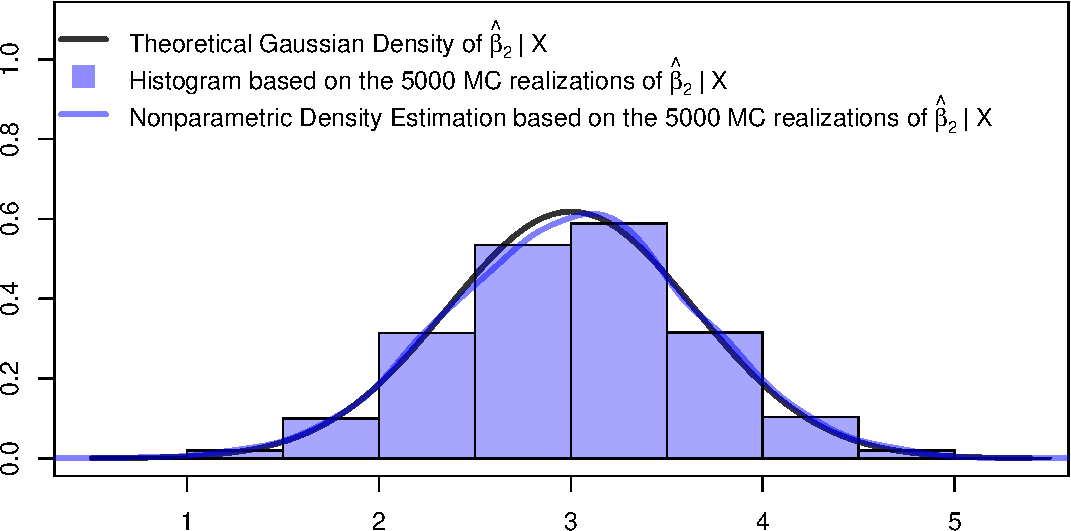
\includegraphics{./05-Small-Sample-Inference_files/figure-pdf/unnamed-chunk-13-1.pdf}

}

\end{figure}

Great! The nonparametric density estimation (estimated via
\texttt{density()}) and the histogram computed based on the 5000
simulated realizations of \(\hat\beta_2|X\) are indicating that
\(\hat\beta_2|X\) is really normally distributed as described by our
theoretical result in Equation Equation~\ref{eq-ssnorm}.

However, what would happen if we would sample \emph{unconditionally} on
\(X\)? How does the distribution of \(\hat\beta_2\) would then look
like?

\begin{Shaded}
\begin{Highlighting}[]
\FunctionTok{set.seed}\NormalTok{(}\DecValTok{1110}\NormalTok{)}
\DocumentationTok{\#\# Let\textquotesingle{}s generate 5000 realizations from beta\_hat\_2 }
\DocumentationTok{\#\# WITHOUT conditioning on X}
\NormalTok{beta\_hat\_2\_uncond }\OtherTok{\textless{}{-}} \FunctionTok{rep}\NormalTok{(}\ConstantTok{NA}\NormalTok{, }\AttributeTok{times=}\NormalTok{rep)}
\DocumentationTok{\#\#}
\ControlFlowTok{for}\NormalTok{(r }\ControlFlowTok{in} \DecValTok{1}\SpecialCharTok{:}\NormalTok{rep)\{}
\NormalTok{    MC\_data }\OtherTok{\textless{}{-}} \FunctionTok{myDataGenerator}\NormalTok{(}\AttributeTok{n    =}\NormalTok{ n, }
                               \AttributeTok{beta =}\NormalTok{ beta\_true)}
\NormalTok{    lm\_obj               }\OtherTok{\textless{}{-}} \FunctionTok{lm}\NormalTok{(Y }\SpecialCharTok{\textasciitilde{}}\NormalTok{ X\_2 }\SpecialCharTok{+}\NormalTok{ X\_3, }\AttributeTok{data =}\NormalTok{ MC\_data)}
\NormalTok{    beta\_hat\_2\_uncond[r] }\OtherTok{\textless{}{-}} \FunctionTok{coef}\NormalTok{(lm\_obj)[}\DecValTok{2}\NormalTok{]}
\NormalTok{\}}

\DocumentationTok{\#\# Compare:}
\DocumentationTok{\#\# True beta\_2 versus average of beta\_hat\_2 estimates}
\FunctionTok{c}\NormalTok{(beta\_true\_2, }\FunctionTok{round}\NormalTok{(}\FunctionTok{mean}\NormalTok{(beta\_hat\_2\_uncond), }\DecValTok{4}\NormalTok{))}
\end{Highlighting}
\end{Shaded}

\begin{verbatim}
[1] 3.0000 3.0078
\end{verbatim}

OK, at least on average the point point estimates are basically equal to
the true parameter value.

\begin{Shaded}
\begin{Highlighting}[]
\DocumentationTok{\#\# Compare: }
\DocumentationTok{\#\# True variance of beta\_hat\_2 versus }
\DocumentationTok{\#\# empirical variance of beta\_hat\_2 estimates}
\FunctionTok{c}\NormalTok{(}\FunctionTok{round}\NormalTok{(var\_true\_beta\_2, }\DecValTok{4}\NormalTok{), }\FunctionTok{round}\NormalTok{(}\FunctionTok{var}\NormalTok{(beta\_hat\_2\_uncond), }\DecValTok{4}\NormalTok{))}
\end{Highlighting}
\end{Shaded}

\begin{verbatim}
[1] 0.4160 0.2478
\end{verbatim}

Ouch! The theoretical variance of \(\hat\beta_2|X\) is quite different
from the actual variance of \(\hat\beta_2\) (i.e.~simulated without
conditioning in \(X\)). That is, we cannot simply neglect that the
variance of \(\hat\beta_2\) depends on the observed realization of \(X\)
in small samples.

\begin{Shaded}
\begin{Highlighting}[]
\DocumentationTok{\#\# Plotting the theoretical distribution of beta\_hat\_2|X }
\DocumentationTok{\#\# versus the simulated distribution}
\FunctionTok{curve}\NormalTok{(}\AttributeTok{expr =} \FunctionTok{dnorm}\NormalTok{(x, }\AttributeTok{mean =}\NormalTok{ beta\_true\_2, }\AttributeTok{sd=}\FunctionTok{sqrt}\NormalTok{(var\_true\_beta\_2)), }
      \AttributeTok{xlab=}\StringTok{""}\NormalTok{,}\AttributeTok{ylab=}\StringTok{""}\NormalTok{, }\AttributeTok{col=}\FunctionTok{gray}\NormalTok{(.}\DecValTok{2}\NormalTok{), }\AttributeTok{lwd=}\DecValTok{3}\NormalTok{, }\AttributeTok{lty=}\DecValTok{1}\NormalTok{, }
      \AttributeTok{xlim=}\FunctionTok{range}\NormalTok{(beta\_hat\_2\_uncond), }\AttributeTok{ylim=}\FunctionTok{c}\NormalTok{(}\DecValTok{0}\NormalTok{,}\FloatTok{1.5}\NormalTok{))}
\FunctionTok{hist}\NormalTok{(beta\_hat\_2\_uncond, }\AttributeTok{freq=}\ConstantTok{FALSE}\NormalTok{, }\AttributeTok{col=}\FunctionTok{alpha}\NormalTok{(}\StringTok{"blue"}\NormalTok{,.}\DecValTok{35}\NormalTok{), }\AttributeTok{add=}\ConstantTok{TRUE}\NormalTok{)}
\FunctionTok{lines}\NormalTok{(}\FunctionTok{density}\NormalTok{(beta\_hat\_2\_uncond, }\AttributeTok{bw=}\FunctionTok{bw.SJ}\NormalTok{(beta\_hat\_2\_uncond)), }
      \AttributeTok{col=}\FunctionTok{alpha}\NormalTok{(}\StringTok{"blue"}\NormalTok{,.}\DecValTok{5}\NormalTok{), }\AttributeTok{lwd=}\DecValTok{3}\NormalTok{)}
\FunctionTok{legend}\NormalTok{(}\StringTok{"topleft"}\NormalTok{, }\AttributeTok{lty=}\FunctionTok{c}\NormalTok{(}\DecValTok{1}\NormalTok{,}\ConstantTok{NA}\NormalTok{,}\DecValTok{1}\NormalTok{), }\AttributeTok{lwd=}\FunctionTok{c}\NormalTok{(}\DecValTok{3}\NormalTok{,}\ConstantTok{NA}\NormalTok{,}\DecValTok{3}\NormalTok{), }\AttributeTok{pch=}\FunctionTok{c}\NormalTok{(}\ConstantTok{NA}\NormalTok{,}\DecValTok{15}\NormalTok{,}\ConstantTok{NA}\NormalTok{), }\AttributeTok{pt.cex=}\FunctionTok{c}\NormalTok{(}\ConstantTok{NA}\NormalTok{,}\DecValTok{2}\NormalTok{,}\ConstantTok{NA}\NormalTok{),}
     \AttributeTok{col=}\FunctionTok{c}\NormalTok{(}\FunctionTok{gray}\NormalTok{(.}\DecValTok{2}\NormalTok{), }\FunctionTok{alpha}\NormalTok{(}\StringTok{"blue"}\NormalTok{,.}\DecValTok{45}\NormalTok{), }\FunctionTok{alpha}\NormalTok{(}\StringTok{"blue"}\NormalTok{,.}\DecValTok{5}\NormalTok{)), }\AttributeTok{bty=}\StringTok{"n"}\NormalTok{, }\AttributeTok{legend=} 
\FunctionTok{c}\NormalTok{(}\FunctionTok{expression}\NormalTok{(}
  \StringTok{"Theoretical Gaussian Density of"}\SpecialCharTok{\textasciitilde{}}\FunctionTok{hat}\NormalTok{(beta)[}\DecValTok{2}\NormalTok{]}\SpecialCharTok{\textasciitilde{}}\StringTok{\textquotesingle{}|\textquotesingle{}}\SpecialCharTok{\textasciitilde{}}\NormalTok{X), }
\FunctionTok{expression}\NormalTok{(}
  \StringTok{"Histogram based on the 5000 MC realizations of"}\SpecialCharTok{\textasciitilde{}}
  \FunctionTok{hat}\NormalTok{(beta)[}\DecValTok{2}\NormalTok{]), }
\FunctionTok{expression}\NormalTok{(}\StringTok{"Nonparam. Density Estimation based on the 5000 MC realizations of"}\SpecialCharTok{\textasciitilde{}}
  \FunctionTok{hat}\NormalTok{(beta)[}\DecValTok{2}\NormalTok{])))}
\end{Highlighting}
\end{Shaded}

\begin{figure}[H]

{\centering 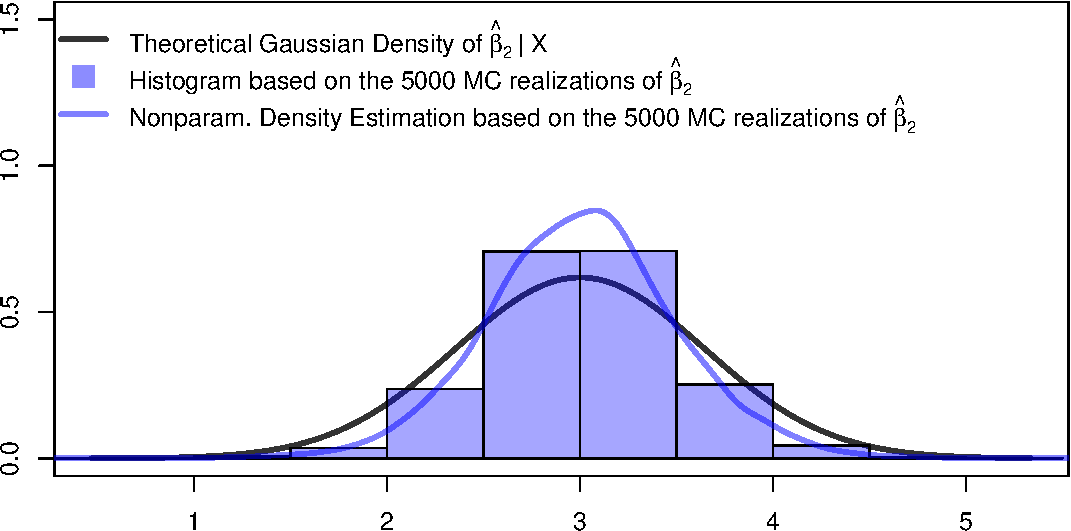
\includegraphics{./05-Small-Sample-Inference_files/figure-pdf/unnamed-chunk-16-1.pdf}

}

\end{figure}

Not so good. The theoretical distribution of \(\hat\beta_2|X\) has much
fatter tails than the simulated distribution of \(\hat\beta_2\)
(i.e.~simulated without conditioning in \(X\)). That is, we cannot
simply neglect that the distribution of \(\hat\beta_2\) depends on the
observed realization of \(X\) in small samples. In large sample,
however, the effect of a given realization \(X\) is (fortunately)
negligible, as we will see in Chapter~\ref{sec-lsinf}.

\hypertarget{testing-multiple-parameters}{%
\subsection{Testing Multiple
Parameters}\label{testing-multiple-parameters}}

In the following, we do inference about multiple parameters. We test
\begin{align*}
H_0:\;&\beta_2=3\quad\text{and}\quad\beta_3=4\\
\text{versus}\quad H_A:\;&\beta_2\neq 3\quad\text{and/or}\quad\beta_3\neq 4.
\end{align*} Or equivalently \begin{align*}
H_0:\;&R\beta -r = 0 \\
H_A:\;&R\beta -r \neq 0,
\end{align*} where

\[
R=\left(
\begin{matrix}
0&1&0\\
0&0&1\\
\end{matrix}\right)\quad\text{ and }\quad 
r=\left(\begin{matrix}3\\4\\\end{matrix}\right).
\]

The following \texttt{R} code can be used to test this hypothesis:

\begin{Shaded}
\begin{Highlighting}[]
\FunctionTok{suppressMessages}\NormalTok{(}\FunctionTok{library}\NormalTok{(}\StringTok{"car"}\NormalTok{)) }\CommentTok{\# for linearHyothesis()}
\CommentTok{\# ?linearHypothesis}

\DocumentationTok{\#\# Estimate the linear regression model parameters}
\NormalTok{lm\_obj }\OtherTok{\textless{}{-}} \FunctionTok{lm}\NormalTok{(Y }\SpecialCharTok{\textasciitilde{}}\NormalTok{ X\_2 }\SpecialCharTok{+}\NormalTok{ X\_3, }\AttributeTok{data =}\NormalTok{ mydata)}

\DocumentationTok{\#\# Option 1:}
\NormalTok{car}\SpecialCharTok{::}\FunctionTok{linearHypothesis}\NormalTok{(}\AttributeTok{model =}\NormalTok{ lm\_obj, }
                      \AttributeTok{hypothesis.matrix =} \FunctionTok{c}\NormalTok{(}\StringTok{"X\_2=3"}\NormalTok{, }\StringTok{"X\_3=4"}\NormalTok{))}
\end{Highlighting}
\end{Shaded}

\begin{verbatim}
Linear hypothesis test

Hypothesis:
X_2 = 3
X_3 = 4

Model 1: restricted model
Model 2: Y ~ X_2 + X_3

  Res.Df    RSS Df Sum of Sq      F  Pr(>F)  
1      9 87.285                              
2      7 37.599  2    49.686 4.6252 0.05246 .
---
Signif. codes:  0 '***' 0.001 '**' 0.01 '*' 0.05 '.' 0.1 ' ' 1
\end{verbatim}

The \(p\)-value is larger than the chosen significance level
\(\alpha=0.05\) thus we cannot reject the null hypothesis.

The following codes gives an alternative, equivalent way to compute the
test result:

\begin{Shaded}
\begin{Highlighting}[]
\DocumentationTok{\#\# Option 2:}
\NormalTok{R }\OtherTok{\textless{}{-}} \FunctionTok{rbind}\NormalTok{(}\FunctionTok{c}\NormalTok{(}\DecValTok{0}\NormalTok{,}\DecValTok{1}\NormalTok{,}\DecValTok{0}\NormalTok{),}
           \FunctionTok{c}\NormalTok{(}\DecValTok{0}\NormalTok{,}\DecValTok{0}\NormalTok{,}\DecValTok{1}\NormalTok{))}
\NormalTok{car}\SpecialCharTok{::}\FunctionTok{linearHypothesis}\NormalTok{(}\AttributeTok{model =}\NormalTok{ lm\_obj, }
                      \AttributeTok{hypothesis.matrix =}\NormalTok{ R, }
                      \AttributeTok{rhs =} \FunctionTok{c}\NormalTok{(}\DecValTok{3}\NormalTok{,}\DecValTok{4}\NormalTok{))}
\end{Highlighting}
\end{Shaded}

\begin{verbatim}
Linear hypothesis test

Hypothesis:
X_2 = 3
X_3 = 4

Model 1: restricted model
Model 2: Y ~ X_2 + X_3

  Res.Df    RSS Df Sum of Sq      F  Pr(>F)  
1      9 87.285                              
2      7 37.599  2    49.686 4.6252 0.05246 .
---
Signif. codes:  0 '***' 0.001 '**' 0.01 '*' 0.05 '.' 0.1 ' ' 1
\end{verbatim}

Again, we cannot reject the null hypothesis at a significance level of,
for instance, \(\alpha=0.05\) since we actually test the true null
hypothesis. However, in repeated samples we should nevertheless observe
\(\alpha\cdot 100\%\) type I errors (false rejections of \(H_0\)). Let's
check this using the following Monte Carlo simulation:

\begin{Shaded}
\begin{Highlighting}[]
\DocumentationTok{\#\# Let\textquotesingle{}s generate 5000 F{-}test decisions and check }
\DocumentationTok{\#\# whether the empirical rate of type I errors is }
\DocumentationTok{\#\# close to the theoretical significance level. }
\NormalTok{rep             }\OtherTok{\textless{}{-}} \DecValTok{5000} \CommentTok{\# MC replications}
\NormalTok{F\_test\_pvalues  }\OtherTok{\textless{}{-}} \FunctionTok{rep}\NormalTok{(}\ConstantTok{NA}\NormalTok{, }\AttributeTok{times=}\NormalTok{rep)}
\DocumentationTok{\#\#}
\ControlFlowTok{for}\NormalTok{(r }\ControlFlowTok{in} \DecValTok{1}\SpecialCharTok{:}\NormalTok{rep)\{}
  \DocumentationTok{\#\# generate new MC\_data conditionally on X\_cond}
\NormalTok{    MC\_data }\OtherTok{\textless{}{-}} \FunctionTok{myDataGenerator}\NormalTok{(}\AttributeTok{n    =}\NormalTok{ n, }
                               \AttributeTok{beta =}\NormalTok{ beta\_true, }
                               \AttributeTok{X    =}\NormalTok{ X\_cond)}
\NormalTok{    lm\_obj            }\OtherTok{\textless{}{-}} \FunctionTok{lm}\NormalTok{(Y }\SpecialCharTok{\textasciitilde{}}\NormalTok{ X\_2 }\SpecialCharTok{+}\NormalTok{ X\_3, }\AttributeTok{data =}\NormalTok{ MC\_data)}
    \DocumentationTok{\#\# save the p{-}value}
\NormalTok{    p }\OtherTok{\textless{}{-}} \FunctionTok{linearHypothesis}\NormalTok{(lm\_obj, }
                          \FunctionTok{c}\NormalTok{(}\StringTok{"X\_2=3"}\NormalTok{, }\StringTok{"X\_3=4"}\NormalTok{))}\SpecialCharTok{$}\StringTok{\textasciigrave{}}\AttributeTok{Pr(\textgreater{}F)}\StringTok{\textasciigrave{}}\NormalTok{[}\DecValTok{2}\NormalTok{]}
\NormalTok{    F\_test\_pvalues[r] }\OtherTok{\textless{}{-}}\NormalTok{ p}
\NormalTok{\}}
\DocumentationTok{\#\#}
\NormalTok{signif\_level }\OtherTok{\textless{}{-}}  \FloatTok{0.05}
\NormalTok{rejections   }\OtherTok{\textless{}{-}}\NormalTok{ F\_test\_pvalues[F\_test\_pvalues }\SpecialCharTok{\textless{}}\NormalTok{ signif\_level]}
\FunctionTok{round}\NormalTok{(}\FunctionTok{length}\NormalTok{(rejections)}\SpecialCharTok{/}\NormalTok{rep, }\DecValTok{4}\NormalTok{)}
\end{Highlighting}
\end{Shaded}

\begin{verbatim}
[1] 0.047
\end{verbatim}

\begin{Shaded}
\begin{Highlighting}[]
\DocumentationTok{\#\# }
\NormalTok{signif\_level }\OtherTok{\textless{}{-}}  \FloatTok{0.01}
\NormalTok{rejections   }\OtherTok{\textless{}{-}}\NormalTok{ F\_test\_pvalues[F\_test\_pvalues }\SpecialCharTok{\textless{}}\NormalTok{ signif\_level]}
\FunctionTok{round}\NormalTok{(}\FunctionTok{length}\NormalTok{(rejections)}\SpecialCharTok{/}\NormalTok{rep, }\DecValTok{4}\NormalTok{)}
\end{Highlighting}
\end{Shaded}

\begin{verbatim}
[1] 0.0092
\end{verbatim}

Note that this is actually a very strong result. First, it means that we
correctly control for the type I error rate since the type I error rate
is not larger than the chosen significance level \(\alpha\). Second, it
means that the test is not conservative (i.e.~very efficient) since the
empirical type I error rate is really close to the chosen significance
level \(\alpha\). (In fact, if we would increase the number of Monte
Carlo repetitions, the empirical type I error rate would converge to the
selected significance level \(\alpha\) due to the law of large numbers.)

Next, we check how well the \(F\) test detects certain violations of the
null hypothesis. We do this by using the same data generating process,
but by testing the following incorrect null hypothesis: \begin{align*}
H_0:\;&\beta_2=4\quad\text{and}\quad\beta_3=4\\
H_A:\;&\beta_2\neq 4\quad\text{and/or}\quad\beta_3\neq 4
\end{align*}

\begin{Shaded}
\begin{Highlighting}[]
\FunctionTok{set.seed}\NormalTok{(}\DecValTok{321}\NormalTok{)}
\NormalTok{rep             }\OtherTok{\textless{}{-}} \DecValTok{5000} \CommentTok{\# MC replications}
\NormalTok{F\_test\_pvalues  }\OtherTok{\textless{}{-}} \FunctionTok{rep}\NormalTok{(}\ConstantTok{NA}\NormalTok{, }\AttributeTok{times=}\NormalTok{rep)}
\DocumentationTok{\#\#}
\ControlFlowTok{for}\NormalTok{(r }\ControlFlowTok{in} \DecValTok{1}\SpecialCharTok{:}\NormalTok{rep)\{}
  \DocumentationTok{\#\# generate new MC\_data conditionally on X\_cond}
\NormalTok{    MC\_data }\OtherTok{\textless{}{-}} \FunctionTok{myDataGenerator}\NormalTok{(}\AttributeTok{n    =}\NormalTok{ n, }
                               \AttributeTok{beta =}\NormalTok{ beta\_true, }
                               \AttributeTok{X    =}\NormalTok{ X\_cond)}
\NormalTok{    lm\_obj            }\OtherTok{\textless{}{-}} \FunctionTok{lm}\NormalTok{(Y }\SpecialCharTok{\textasciitilde{}}\NormalTok{ X\_2 }\SpecialCharTok{+}\NormalTok{ X\_3, }\AttributeTok{data =}\NormalTok{ MC\_data)}
    \DocumentationTok{\#\# save p{-}values of all rep{-}many tests}
\NormalTok{    F\_test\_pvalues[r] }\OtherTok{\textless{}{-}} \FunctionTok{linearHypothesis}\NormalTok{(lm\_obj,}
                         \FunctionTok{c}\NormalTok{(}\StringTok{"X\_2=4"}\NormalTok{,}\StringTok{"X\_3=4"}\NormalTok{))}\SpecialCharTok{$}\StringTok{\textasciigrave{}}\AttributeTok{Pr(\textgreater{}F)}\StringTok{\textasciigrave{}}\NormalTok{[}\DecValTok{2}\NormalTok{]}
\NormalTok{\}}
\DocumentationTok{\#\#}
\NormalTok{signif\_level }\OtherTok{\textless{}{-}}  \FloatTok{0.05}
\NormalTok{rejections   }\OtherTok{\textless{}{-}}\NormalTok{ F\_test\_pvalues[F\_test\_pvalues }\SpecialCharTok{\textless{}}\NormalTok{ signif\_level]}
\FunctionTok{length}\NormalTok{(rejections)}\SpecialCharTok{/}\NormalTok{rep}
\end{Highlighting}
\end{Shaded}

\begin{verbatim}
[1] 0.3924
\end{verbatim}

Indeed, we can now reject the (here false) null hypothesis in
approximately \(39\%\) of all resamplings from the true data generating
process. \textbf{Caution:} This also means that we are not able to
``see'' the violation of the null hypothesis in \(100\%-39\%=62\%\) of
cases. Therefore, we can never use an insignificant test result
(p-value\(\geq\alpha\)) as a justification to accept the null
hypothesis. Obviously, there are Type II error events, but since we
typically do not know the distribution of the test statistic under the
alternative hypothesis, we cannot control the Type II error rate. We can
only control the Type I error rate by using a small significance level
\(\alpha\).

Moreover, note that the \(F\) test is not informative about which part
of the null hypothesis (\(\beta_2=4\) and/or \(\beta_3=4\)) is violated
-- we only get the information that at least one of the multiple
parameter hypotheses is violated:

\begin{Shaded}
\begin{Highlighting}[]
\NormalTok{car}\SpecialCharTok{::}\FunctionTok{linearHypothesis}\NormalTok{(lm\_obj, }\FunctionTok{c}\NormalTok{(}\StringTok{"X\_2=4"}\NormalTok{, }\StringTok{"X\_3=4"}\NormalTok{))}
\end{Highlighting}
\end{Shaded}

\begin{verbatim}
Linear hypothesis test

Hypothesis:
X_2 = 4
X_3 = 4

Model 1: restricted model
Model 2: Y ~ X_2 + X_3

  Res.Df     RSS Df Sum of Sq      F   Pr(>F)   
1      9 141.245                                
2      7  32.572  2    108.67 11.677 0.005889 **
---
Signif. codes:  0 '***' 0.001 '**' 0.01 '*' 0.05 '.' 0.1 ' ' 1
\end{verbatim}

\hypertarget{dualty-of-confidence-intervals-and-hypothesis-tests}{%
\subsection{Dualty of Confidence Intervals and Hypothesis
Tests}\label{dualty-of-confidence-intervals-and-hypothesis-tests}}

Confidence intervals can be computed using \texttt{R} as following:

\begin{Shaded}
\begin{Highlighting}[]
\NormalTok{signif\_level }\OtherTok{\textless{}{-}} \FloatTok{0.05}
\DocumentationTok{\#\# 95\% CI for beta\_2}
\FunctionTok{confint}\NormalTok{(lm\_obj, }\AttributeTok{parm =} \StringTok{"X\_2"}\NormalTok{, }\AttributeTok{level =} \DecValTok{1} \SpecialCharTok{{-}}\NormalTok{ signif\_level)}
\end{Highlighting}
\end{Shaded}

\begin{verbatim}
       2.5 %   97.5 %
X_2 1.370315 3.563536
\end{verbatim}

\begin{Shaded}
\begin{Highlighting}[]
\DocumentationTok{\#\# 95\% CI for beta\_3 }
\FunctionTok{confint}\NormalTok{(lm\_obj, }\AttributeTok{parm =} \StringTok{"X\_3"}\NormalTok{, }\AttributeTok{level =} \DecValTok{1} \SpecialCharTok{{-}}\NormalTok{ signif\_level)}
\end{Highlighting}
\end{Shaded}

\begin{verbatim}
       2.5 %   97.5 %
X_3 3.195389 4.695134
\end{verbatim}

We can use these two-sided confidence intervals to do hypothesis tests.
For instance, when testing the null hypothesis \begin{align*}
H_0:&\beta_3=4\\
\text{versus}\quad H_A: &\beta_3\neq 4
\end{align*} we can check whether the confidence interval
\(\operatorname{CI}_{1-\alpha}\) contains the hypothetical value \(4\)
or not. In case of \(4\in \operatorname{CI}_{1-\alpha}\), we cannot
reject the null hypothesis. In case of
\(4\not\in \operatorname{CI}_{1-\alpha}\), we reject the null
hypothesis.

If the Assumption 1-4\(^\ast\) hold true, then
\(\operatorname{CI}_{1-\alpha}\) is an exact confidence interval. That
is, under the null hypothesis, it falsely rejects the null hypothesis in
only \(\alpha\cdot 100\%\) of resamplings. Let's check this in the
following \texttt{R} code:

\begin{Shaded}
\begin{Highlighting}[]
\DocumentationTok{\#\# Let\textquotesingle{}s generate 1000 CIs }
\FunctionTok{set.seed}\NormalTok{(}\DecValTok{123}\NormalTok{)}
\NormalTok{signif\_level }\OtherTok{\textless{}{-}}  \FloatTok{0.05}
\NormalTok{rep          }\OtherTok{\textless{}{-}} \DecValTok{5000} \CommentTok{\# MC replications}
\NormalTok{confint\_m    }\OtherTok{\textless{}{-}} \FunctionTok{matrix}\NormalTok{(}\ConstantTok{NA}\NormalTok{, }\AttributeTok{nrow=}\DecValTok{2}\NormalTok{, }\AttributeTok{ncol=}\NormalTok{rep)}
\DocumentationTok{\#\#}
\ControlFlowTok{for}\NormalTok{(r }\ControlFlowTok{in} \DecValTok{1}\SpecialCharTok{:}\NormalTok{rep)\{}
  \DocumentationTok{\#\# generate new MC\_data conditionally on X\_cond}
\NormalTok{    MC\_data }\OtherTok{\textless{}{-}} \FunctionTok{myDataGenerator}\NormalTok{(}\AttributeTok{n    =}\NormalTok{ n, }
                               \AttributeTok{beta =}\NormalTok{ beta\_true, }
                               \AttributeTok{X    =}\NormalTok{ X\_cond)}
\NormalTok{    lm\_obj            }\OtherTok{\textless{}{-}} \FunctionTok{lm}\NormalTok{(Y }\SpecialCharTok{\textasciitilde{}}\NormalTok{ X\_2 }\SpecialCharTok{+}\NormalTok{ X\_3, }\AttributeTok{data =}\NormalTok{ MC\_data)}
    \DocumentationTok{\#\# save the p{-}value}
\NormalTok{    CI }\OtherTok{\textless{}{-}} \FunctionTok{confint}\NormalTok{(lm\_obj, }\AttributeTok{parm=}\StringTok{"X\_2"}\NormalTok{, }\AttributeTok{level=}\DecValTok{1}\SpecialCharTok{{-}}\NormalTok{signif\_level)}
\NormalTok{    confint\_m[,r] }\OtherTok{\textless{}{-}}\NormalTok{ CI}
\NormalTok{\}}
\DocumentationTok{\#\#}
\NormalTok{inside\_CI  }\OtherTok{\textless{}{-}}\NormalTok{ confint\_m[}\DecValTok{1}\NormalTok{,] }\SpecialCharTok{\textless{}=}\NormalTok{ beta\_true\_2 }\SpecialCharTok{\&} 
\NormalTok{                beta\_true\_2 }\SpecialCharTok{\textless{}=}\NormalTok{ confint\_m[}\DecValTok{2}\NormalTok{,]}

\DocumentationTok{\#\# CI{-}lower, CI{-}upper, beta\_true\_2 inside?}
\FunctionTok{head}\NormalTok{(}\FunctionTok{cbind}\NormalTok{(}\FunctionTok{t}\NormalTok{(confint\_m), inside\_CI))}
\end{Highlighting}
\end{Shaded}

\begin{verbatim}
                        inside_CI
[1,] 0.8555396 3.639738         1
[2,] 0.9143542 3.270731         1
[3,] 1.9336526 4.984167         1
[4,] 1.9985874 3.812695         1
[5,] 3.0108642 5.621791         0
[6,] 2.0967675 4.716398         1
\end{verbatim}

The following code computes the relative frequency of confidence
intervals \textbf{not containing} the true parameter value
\((\beta_2=3)\):

\begin{Shaded}
\begin{Highlighting}[]
\FunctionTok{round}\NormalTok{(}\FunctionTok{length}\NormalTok{(inside\_CI[inside\_CI }\SpecialCharTok{==} \ConstantTok{FALSE}\NormalTok{])}\SpecialCharTok{/}\NormalTok{rep, }\DecValTok{4}\NormalTok{)}
\end{Highlighting}
\end{Shaded}

\begin{verbatim}
[1] 0.0516
\end{verbatim}

That's good! The relative frequency is basically equal to the chosen
\(\alpha=0.05\) value.

Next, we visualize a sample of \texttt{nCIs\ \textless{}-\ 100}
realizations of the random confidence interval:

\begin{Shaded}
\begin{Highlighting}[]
\NormalTok{nCIs }\OtherTok{\textless{}{-}} \DecValTok{100}
\FunctionTok{plot}\NormalTok{(}\AttributeTok{x=}\DecValTok{0}\NormalTok{,}\AttributeTok{y=}\DecValTok{0}\NormalTok{,}\AttributeTok{type=}\StringTok{"n"}\NormalTok{,}\AttributeTok{xlim=}\FunctionTok{c}\NormalTok{(}\DecValTok{0}\NormalTok{,nCIs),}\AttributeTok{ylim=}\FunctionTok{range}\NormalTok{(confint\_m[,}\DecValTok{1}\SpecialCharTok{:}\NormalTok{nCIs]),}
     \AttributeTok{ylab=}\StringTok{""}\NormalTok{, }\AttributeTok{xlab=}\StringTok{"Resamplings"}\NormalTok{, }\AttributeTok{main=}\StringTok{"Confidence Intervals"}\NormalTok{)}
\ControlFlowTok{for}\NormalTok{(r }\ControlFlowTok{in} \DecValTok{1}\SpecialCharTok{:}\NormalTok{nCIs)\{}
  \ControlFlowTok{if}\NormalTok{(inside\_CI[r]}\SpecialCharTok{==}\ConstantTok{TRUE}\NormalTok{)\{}
      \FunctionTok{lines}\NormalTok{(}\AttributeTok{x=}\FunctionTok{c}\NormalTok{(r,r), }\AttributeTok{y=}\FunctionTok{c}\NormalTok{(confint\_m[}\DecValTok{1}\NormalTok{,r], confint\_m[}\DecValTok{2}\NormalTok{,r]), }
            \AttributeTok{lwd=}\DecValTok{2}\NormalTok{, }\AttributeTok{col=}\FunctionTok{gray}\NormalTok{(.}\DecValTok{5}\NormalTok{,.}\DecValTok{5}\NormalTok{))}
\NormalTok{  \}}\ControlFlowTok{else}\NormalTok{\{}
      \FunctionTok{lines}\NormalTok{(}\AttributeTok{x=}\FunctionTok{c}\NormalTok{(r,r), }\AttributeTok{y=}\FunctionTok{c}\NormalTok{(confint\_m[}\DecValTok{1}\NormalTok{,r], confint\_m[}\DecValTok{2}\NormalTok{,r]), }
            \AttributeTok{lwd=}\DecValTok{2}\NormalTok{, }\AttributeTok{col=}\StringTok{"darkred"}\NormalTok{)}
\NormalTok{    \}}
\NormalTok{\}}
\FunctionTok{axis}\NormalTok{(}\DecValTok{4}\NormalTok{, }\AttributeTok{at=}\NormalTok{beta\_true\_2, }\AttributeTok{labels =} \FunctionTok{expression}\NormalTok{(beta[}\DecValTok{2}\NormalTok{]))}
\FunctionTok{abline}\NormalTok{(}\AttributeTok{h=}\NormalTok{beta\_true\_2)}
\end{Highlighting}
\end{Shaded}

\begin{figure}[H]

{\centering 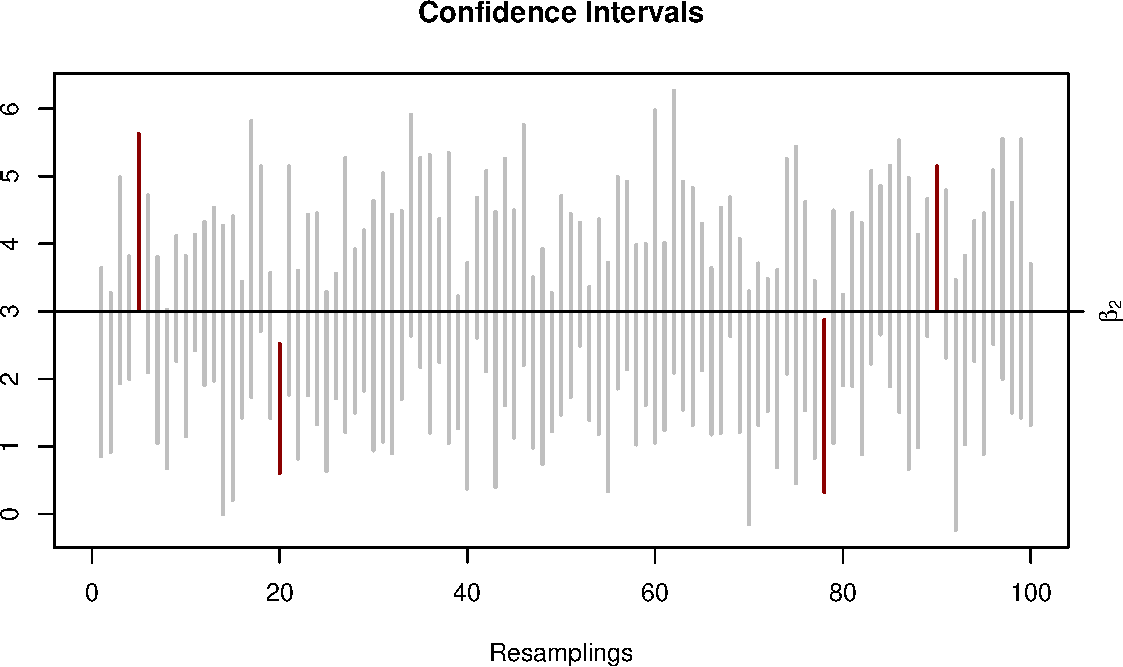
\includegraphics{./05-Small-Sample-Inference_files/figure-pdf/unnamed-chunk-25-1.pdf}

}

\end{figure}

As expected, only about \(\alpha\cdot 100\%=5\%\) of all confidence
intervals do not contain the true parameter value \(\beta_2=3\), but
about \((1-\alpha)\cdot 100\%=95\%\) of all confidence intervals contain
the true parameter value \(\beta_2=3\).

\bookmarksetup{startatroot}

\hypertarget{references-1}{%
\chapter*{References}\label{references-1}}
\addcontentsline{toc}{chapter}{References}

\bookmarksetup{startatroot}

\hypertarget{sec-lsinf}{%
\chapter{Large Sample Inference}\label{sec-lsinf}}

The content of this chapter is very much inspired by the book by Hayashi
(2000).

\hypertarget{tools-for-asymptotic-statistics}{%
\section{Tools for Asymptotic
Statistics}\label{tools-for-asymptotic-statistics}}

\hypertarget{modes-of-convergence}{%
\subsection{Modes of Convergence}\label{modes-of-convergence}}

In the following we will discuss the four most important convergence
concepts for sequences of random variables \((z_1,z_2,\dots,z_n)\)
shortly denoted by \(\{z_n\}\). Non-random scalars (or vectors or
matrices) will be denoted by Greek letters such as \(\alpha\).

\hypertarget{four-important-modes-of-convergence}{%
\subsection*{Four Important Modes of
Convergence}\label{four-important-modes-of-convergence}}
\addcontentsline{toc}{subsection}{Four Important Modes of Convergence}

\leavevmode\vadjust pre{\hypertarget{def-conv_prop}{}}%
\begin{definition}[Convergence in Probability]\label{def-conv_prop}

A sequence of random scalars \(\{z_n\}\) \textbf{converges in
probability} to a constant (non-random) \(\alpha\) if, for any
(arbitrarily small) \(\varepsilon>0\), \begin{eqnarray*}
  \lim_{n\to\infty} P\left(|z_n-\alpha|>\varepsilon\right)=0.
\end{eqnarray*} We write:
\(\operatorname{plim}_{n\to\infty}z_n=\alpha\), or \(z_n\to_{p}\alpha\).
Convergence in probability of a sequence of random vectors (or matrices)
\(\{z_n\}\) to a constant vector (or matrix) \(\alpha\) requires
\emph{element-wise} convergence in probability.

\end{definition}

\leavevmode\vadjust pre{\hypertarget{def-conv_as}{}}%
\begin{definition}[Almost Sure Convergence]\label{def-conv_as}

A sequence of random scalars \(\{z_n\}\) \textbf{converges almost
surely} to a constant (non-random) \(\alpha\) if \begin{eqnarray*}
P\left(\lim_{n\to\infty}z_n=\alpha\right)=1.
\end{eqnarray*} We write: \(z_n\to_{as}\alpha\). Almost sure convergence
of a sequence of random vectors (or matrices) \(\{z_n\}\) to a constant
vector (or matrix) \(\alpha\) requires \emph{element-wise} almost sure
convergence.

\end{definition}

Almost sure convergence is (usually) rather hard to derive, since the
probability is about an event concerning an infinite sequence.
Fortunately, however, there are established strong laws of large numbers
that we can use for showing almost sure convergence.

\leavevmode\vadjust pre{\hypertarget{def-conv_ms}{}}%
\begin{definition}[Convergence in Mean Square]\label{def-conv_ms}

A sequence of random scalars \(\{z_n\}\) \textbf{converges in mean
square} (or \textbf{in quadratic mean}) to a constant (non-random)
\(\alpha\) if \begin{eqnarray*}
  \lim_{n\to\infty}E\left((z_n-\alpha)^2\right)=0
\end{eqnarray*} We write: \(z_n\to_{ms}\alpha\). If \(z_n\) is an
estimator (e.g., \(z_n=\hat\beta_{k,n}\)) the expression
\(E\left((z_n-\alpha)^2\right)\) is termed the \textbf{mean squared
error}: \(\text{MSE}(z_n)=E\left((z_n-\alpha)^2\right)\). Mean square
convergence of a sequence of random vectors (or matrices) \(\{z_n\}\) to
a deterministic vector (or matrix) \(\alpha\) requires
\emph{element-wise} mean square convergence.

\end{definition}

\leavevmode\vadjust pre{\hypertarget{def-conv_distr}{}}%
\begin{definition}[Convergence in Distribution]\label{def-conv_distr}

Let \(F_n\) be the cumulative distribution function (cdf) of \(z_n\) and
\(F\) the cdf of \(z\). A sequence of random scalars \(\{z_n\}\)
\textbf{converges in distribution} to a random scalar \(z\) if for all
\(t\) such that \(F(t)\) is continuous at \(t\), \begin{eqnarray*}
  \lim_{n\to\infty}F_n(t)=F(t).
\end{eqnarray*} We write: \(z_n\to_{d} z\) and call \(F\) the
\textbf{asymptotic} (or \textbf{limit}) \textbf{distribution} of
\(z_n\). Sometimes you will see statements like \(z_n\to_{d} N(0,1)\) or
\(z_n\overset{a}{\sim}N(0,1)\), which should be read as
\(z_n\to_{d} z\), where \(z\sim N(0,1)\).

\end{definition}

A stochastic sequence \(\{z_n\}\) can also convergence in distribution
to a \textbf{deterministic scalar} \(\alpha\). In this case \(\alpha\)
is treated as a degenerated random variable with cdf

\[
F_\alpha(t)=\left\{\begin{matrix}0&\text{if}\;\;t<\alpha\\ 1&\text{if}\;\;t\geq\alpha\end{matrix}\right.
\]

\leavevmode\vadjust pre{\hypertarget{def-conv_multdistr}{}}%
\begin{definition}[Multivariate Convergence in
Distribution]\label{def-conv_multdistr}

Let \(z_n,z\in\mathbb{R}^K\) be \(K\)-dimensional random variables, then

\[
z_n\to_{d} z\text{\quad if and only if \quad}\lambda'z_n\to_{d}\lambda'z
\]

for any \(\lambda\in\mathbb{R}^K\).

\end{definition}

This statement is known as the \textbf{Cramer Wold Device}. It is needed
since element-wise convergence in distribution does generally not imply
convergence of the \emph{joint} distribution of \(z_n\) to the
\emph{joint} distribution of \(z\); except, if all elements are
independent from each other.

\hypertarget{relations-among-modes-of-convergence}{%
\subsection*{Relations among Modes of
Convergence}\label{relations-among-modes-of-convergence}}
\addcontentsline{toc}{subsection}{Relations among Modes of Convergence}

\leavevmode\vadjust pre{\hypertarget{lem-Relations}{}}%
\begin{lemma}[Relationship among the four modes of
convergence]\label{lem-Relations}

The following relationships hold:

\begin{enumerate}
\def\labelenumi{(\roman{enumi})}
\tightlist
\item
  \(z_n\to_{ms}\alpha\Rightarrow z_n\to_{p}\alpha.\)
\item
  \(z_n\to_{as}\alpha\Rightarrow z_n\to_{p}\alpha.\)
\item
  \(z_n\to_{d}\alpha\Leftrightarrow z_n\to_{p}\alpha.\) I.e., if the
  limiting random variable is a constant (i.e., a degenerated random
  variable), then convergence in distribution is equivalent to
  convergence in probability.
\end{enumerate}

\end{lemma}

Proofs can be found, e.g., here:
\url{https://www.statlect.com/asymptotic-theory/relations-among-modes-of-convergence}

\hypertarget{continuous-mapping-theorem-cmt}{%
\subsection{Continuous Mapping Theorem
(CMT)}\label{continuous-mapping-theorem-cmt}}

\leavevmode\vadjust pre{\hypertarget{lem-Preserv}{}}%
\begin{lemma}[Preservation of convergence for continuous transformations
(or ``continuous mapping theorem (CMT)'')]\label{lem-Preserv}

Suppose \(\{z_n\}\) is a stochastic sequence of random scalars, vectors,
or matrices and that \(a(\cdot)\) is a continuous function that does not
depended on \(n\). Then

\begin{enumerate}
\def\labelenumi{(\roman{enumi})}
\tightlist
\item
  \(z_n\to_{p}\alpha\Rightarrow a(z_n)\to_{p} a(\alpha)\)
\item
  \(z_n\to_{as} \alpha\Rightarrow a(z_n)\to_{as} a(\alpha)\)
\item
  \(z_n\to_{d}\alpha\Rightarrow a(z_n)\to_{d} a(\alpha)\)
\end{enumerate}

\end{lemma}

Proof can be found, e.g., in \emph{Asymptotic Statistics}, van der Vaart
(1998), Theorem 2.3. Or here:
\url{https://www.statlect.com/asymptotic-theory/continuous-mapping-theorem}

\textbf{Note:} The CMT does \emph{not} hold for m.s.-convergence except
for the case where \(a(.)\) is linear.\\

\textbf{Examples:} As a consequence of the CMT (Lemma~\ref{lem-Preserv})
we have that the usual arithmetic operations preserve convergence in
probability (equivalently for almost sure convergence and convergence in
distribution):

\begin{itemize}
\tightlist
\item
  If \(x_n\to_{p} \beta\) and \(y_n\to_{p} \gamma\) then
  \(x_n+y_n\to_{p} \beta+\gamma\)
\item
  If \(x_n\to_{p} \beta\) and \(y_n\to_{p} \gamma\) then
  \(x_n\cdot y_n\to_{p} \beta\cdot\gamma\)
\item
  If \(x_n\to_{p} \beta\) and \(y_n\to_{p} \gamma\) then
  \(x_n/y_n\to_{p} \beta/\gamma\), provided that \(\gamma\neq 0\)
\item
  If \(X_n'X_n\to_{p} \Sigma_{X'X}\) then
  \((X_n'X_n)^{-1}\to_{p} \Sigma_{X'X}^{-1}\), provided \(\Sigma_{X'X}\)
  is a nonsingular matrix.
\end{itemize}

\hypertarget{slutsky-theorem}{%
\subsection{Slutsky Theorem}\label{slutsky-theorem}}

The following results are concerned with combinations of convergence in
probability and convergence in distribution. These are particularly
important for the derivation of the asymptotic distribution of
estimators.

\leavevmode\vadjust pre{\hypertarget{lem-Slutsky}{}}%
\begin{lemma}[Slutsky Theorem]\label{lem-Slutsky}

Let \(x_n\) and \(y_n\) denote sequences of random scalars or vectors
and let \(A_n\) denote a sequences of random matrices. Moreover,
\(\alpha\) and \(A\) are deterministic limits of appropriate dimensions
and \(x\) is a random limit of appropriate dimension.

\begin{enumerate}
\def\labelenumi{(\roman{enumi})}
\tightlist
\item
  If \(x_n\to_{d} x\)\quad and \quad \(y_n\to_{p} \alpha\) \quad then;;
  \(x_n+y_n\to_{d} x+\alpha\)
\item
  If \(x_n\to_{d} x\)\quad and \quad \(y_n\to_{p} 0\) \quad then;;
  \(x_n'y_n\to_{p} 0\)
\item
  If \(x_n\to_{d} x\)\quad and \quad \(A_n\to_{p} A\) \quad then;;
  \(A_nx_n\to_{d} Ax\), where it is assumed that \(A_n\) and \(x_n\) are
  ``conformable''(i.e., the matrix- and vector-dimensions fit to each
  other).
\end{enumerate}

Important special case:

If \(x_n\to_{d} N(0,\Sigma)\)\quad and \quad \(A_n\to_{p} A\)
\quad then;; \(A_nx_n\to_{d} N(0,A\Sigma A')\)

\end{lemma}

Proofs can be found, e.g., in \emph{Asymptotic Statistics}, van der
Vaart, Theorem 2.8. Or here:
\url{https://www.statlect.com/asymptotic-theory/Slutsky-theorem}

\textbf{Note:} Sometimes, only parts \emph{(i)} and \emph{(ii)} of
Lemma~\ref{lem-Slutsky} are called ``Slutsky's theorem.''

\hypertarget{law-of-large-numbers-lln-and-central-limit-theorem-clt}{%
\subsection{Law of Large Numbers (LLN) and Central Limit Theorem
(CLT)}\label{law-of-large-numbers-lln-and-central-limit-theorem-clt}}

So far, we discussed the definitions of the four most important
convergence modes, their relations among each other, and basic theorems
(CMT and Slutsky) about functionals of stochastic sequences. Though, we
still lack of tools that allow us to actually show that a stochastic
sequence convergences (in some of the discussed modes) to some limit.

In the following we consider the stochastic sequences \(\{\bar{z}_n\}\)
of sample means \(\bar{z}_n=n^{-1}\sum_{i=1}^nz_i\), where \(z_i\),
\(i=1,\dots,n\), are (scalar, vector, or matrix-valued) \emph{random
variables}. Remember: the sample mean \(\bar{z}_n\) is an estimator of
the deterministic population mean \(\mu\).

Weak LLNs, strong LLNs, and CLTs tell us conditions under which
arithmetic means \(\bar{z}_n=n^{-1}\sum_{i=1}^nz_i\) converge:
\begin{eqnarray*}
  \bar{z}_n&\to_{p}&\mu\quad\text{(weak LLN)}\\
  \bar{z}_n&\to_{as}&\mu\quad\text{(strong LLN)}\\
  \sqrt{n}(\bar{z}_n-\mu)&\to_{d}&N(0,\sigma^2)\quad\text{(CLT)}
\end{eqnarray*}

In the following we introduce the most well-known versions of the weak,
the strong LLN, and the CLT.

\leavevmode\vadjust pre{\hypertarget{thm-WLLN1}{}}%
\begin{theorem}[Weak LLN (Chebychev)]\label{thm-WLLN1}

If \(\lim_{n\to\infty} E(\bar{z}_n)=\mu\) and
\(\lim_{n\to\infty}Var(\bar{z}_n)=0\) then \(\bar{z}_n\to_{p}\mu.\)

\end{theorem}

Proof can be found, for instance, here:
\url{https://www.statlect.com/asymptotic-theory/law-of-large-numbers}

\leavevmode\vadjust pre{\hypertarget{thm-SLLN1}{}}%
\begin{theorem}[Strong LLN (Kolmogorov)]\label{thm-SLLN1}

If \(\{z_i\}\) is an iid sequence and \(E(z_i)=\mu\) then
\(\bar{z}_n\to_{as}\mu.\)

\end{theorem}

Proof can be found, e.g., in \emph{Linear Statistical Inference and Its
Applications}, Rao (1973), pp.~112-114.

\textbf{Note:} The weak and the strong LLN for random vectors follow
from requiring element-by-element convergence.

\leavevmode\vadjust pre{\hypertarget{thm-CLT1}{}}%
\begin{theorem}[CLT (Lindeberg-Levy)]\label{thm-CLT1}

If \(\{z_i\}\) is an iid sequence and \(E(z_i)=\mu\) and
\(Var(z_i)=\sigma^2\) then

\[
\sqrt{n}(\bar{z}_n-\mu)\to_{d} N(0,\sigma^2)\quad\text{as}\quad n\to\infty
\]

\end{theorem}

Proof can be found, e.g., in \emph{Asymptotic Statistics}, van der Vaart
(1998), Theorem 2.17.

The Lindeberg-Levy CLT for \(K\)-dimensional random vectors follows from
our above discussion on ``Multivariate Convergence in
Distribution.''From this we know that if \(\bar{z}_n\in\mathbb{R}^K\)
and \(\mu\in\mathbb{R}^K\), then

\[\sqrt{n}(\bar{z}_n-\mu)\to_{d} \mathcal{N}(0,\Sigma)\quad\Leftrightarrow\quad \sqrt{n}(\lambda'\bar{z}_n-\lambda'\mu)\to_{d} \mathcal{N}(0,\lambda'\Sigma\lambda),\]

for any \(\lambda\in\mathbb{R}^K\).

That is, to apply the Lindeberg-Levy CLT (Theorem~\ref{thm-CLT1}) to
multivariate (e.g., \(K\)-dimensional) stochastic sequences, we need to
check whether the univariate stochastic sequence \(\{\lambda'z_i\}\) is
i.i.d. with \(E(\lambda'z_i)=\lambda'\mu\) and
\(Var(\lambda'z_i)=\lambda'\Sigma\lambda\) for any
\(\lambda\in\mathbb{R}^K\). This is the case if the multivariate
(\(K\)-dimensional) stochastic sequence \(\{z_i\}\) is an i.i.d.
sequence with \(E(z_i)=\mu\) and \(Var(z_i)=\Sigma\).

\textbf{Note:} The LLNs and the CLT are stated with respect to sequences
of sample means \(\{\bar{z}_n\}\); i.e., the simplest estimators you
probably can think of. We will see, however, that this is all we need in
order to analyze also more complicated estimators such as the OLS
estimator.

\hypertarget{estimators-as-a-sequences-of-random-variables}{%
\subsection{Estimators as a Sequences of Random
Variables}\label{estimators-as-a-sequences-of-random-variables}}

Our concepts above readily apply to general scalar-valued (univariate)
or vector-valued (\(K\)-dimensional) estimators, say
\(\hat\theta_n\in\mathbb{R}^K\), that are computed from i.i.d. random
samples.

\textbf{(Weak) Consistency:} We say that an estimator \(\hat\theta_n\)
is \emph{(weakly) consistent for \(\theta\)} if

\[\hat\theta_n\to_{p}\theta\quad\text{as}\quad n\to\infty\]

\textbf{Asymptotic Bias:} The \emph{asymptotic bias} of an estimator
\(\hat\theta_n\) of some true parameter \(\theta\) is defined as:

\[\text{ABias}(\hat\theta_n)=\lim_{n\to\infty}E(\hat\theta_n)-\theta\]

If \(\text{ABias}(\hat\theta_n)=0\), then \(\hat\theta\) is called an
\textbf{asymptotically unbiased}.

\textbf{Asymptotic Normality:} A consistent estimator \(\hat\theta_n\)
is \emph{asymptotically normal distributed} if

\[\sqrt{n}(\hat\theta_n-\theta)\to_{d} \mathcal{N}(0,\Sigma)\quad\text{as}\quad n\to\infty\]

where
\(\lim_{n\to\infty}Var(\sqrt{n}(\hat\theta_n-\theta))=\lim_{n\to\infty}Var(\sqrt{n}\hat\theta_n)=\Sigma\)
as called the asymptotic variance of \(\sqrt{n}(\hat\theta_n-\theta)\).

\textbf{\(\sqrt{n}\)-consistent:} Consistent estimators
\(\hat{\theta}_n\to_{p}\theta\) are called *\(\sqrt{n*\)-consistent\} if

\[\sqrt{n}(\hat\theta_n-\theta)\to_{d} z \quad\text{as}\quad n\to\infty\]

If additionally the random vector \(z\) is normal distributed, then
\(\hat\theta_n\) is often called \emph{consistent and asymptotically
normal.}

\hypertarget{asymptotics-under-the-classic-regression-model}{%
\section{Asymptotics under the Classic Regression
Model}\label{asymptotics-under-the-classic-regression-model}}

Given the above introduced machinery on asymptotic concepts and results,
we can now proof that the OLS estimators \(\hat\beta\) and \(s_{UB}^2\)
applied to the classic regression model (defined by Assumptions 1-4 in
Chapter~\ref{sec-MLR} are both consistent, and that \(\hat\beta\) is
asymptotically normal distributed as \(n\to\infty\). That is, we can
drop the unrealistic normality and spherical errors assumption
(Assumption 4\(^\ast\)), but still use the usual test statistics
(\(t\)-test, \(F\)-test); as long as the sample size \(n\) is ``large.''

However, before we can formally state the asymptotic properties, we,
first, need to adjust our ``data generating process''assumption
(Assumption 1) such that we can apply Kolmogorov's strong LLN and
Lindeberg-Levy's CLT. Second, we need to adjust the rank assumption
(Assumption 3), such that the full column rank of \(X\) is guaranteed
for the limiting case as \(n\to\infty\), too. Assumptions 2 and 4 from
Chapter~\ref{sec-MLR} are assumed to hold (and do not need to be
changed).

\textbf{Assumption 1\(^\ast\): Data Generating Process (for
Asymptotics)} Assumption 1 of Chapter~\ref{sec-MLR} applies, but
\emph{additionally} we assume that
\((\varepsilon_i, X_i)\in\mathbb{R}^{K+1}\) (or equivalently
\((Y_i,X_i)\in\mathbb{R}^{K+1}\)) is jointly i.i.d. for all
\(i=1,\dots,n\), with existing and finite second moments for \(X_i\) and
fourth moments for \(\varepsilon_i\).

\textbf{Note 1:} The fourth moment of \(\varepsilon_i\) is actually only
needed for Theorem~\ref{thm-Consistency_s1}; for the rest two moments
are sufficient.

\textbf{Note 2:} The above adjustment of Assumption 1 is far less
restrictive than assuming that the error-terms \(\varepsilon_i\) are
i.i.d. normally distributed and independent from \(X_i\) (as it's
necessary for small sample inference in Chapter~\ref{sec-ssinf}).

\textbf{Assumption 3\(^\ast\): Rank Condition (for Asymptotics)} The
\((K\times K)\) matrix

\[\Sigma_{X'X}:=E(S_{X'X})=E(n^{-1}X'X)=E(X_iX_i')\]

has full rank \(K\). I.e., \(\Sigma_{X'X}\) is nonsingular and
invertible.

\leavevmode\vadjust pre{\hypertarget{thm-Sxx1}{}}%
\begin{theorem}[Consistency of \(S_{X'X}^{-1}\)]\label{thm-Sxx1}

Under Assumption 1\(^\ast\) and 3\(^\ast\) we have that

\[\left(\frac{1}{n}X'X\right)^{-1}=S_{X'X}^{-1}\quad\to_{p}\quad\Sigma_{X'X}^{-1}\quad\text{as}\quad n\to\infty\]

\end{theorem}

Proof is done in the lecture.

\leavevmode\vadjust pre{\hypertarget{thm-bconsistent1}{}}%
\begin{theorem}[Consistency of \(\hat\beta\)]\label{thm-bconsistent1}

Under Assumption 1\(^\ast\), 2 and 3\(^\ast\) we have that

\[\hat\beta_n\to_{p}\beta\quad\text{as}\quad n\to\infty\]

\end{theorem}

Proof is done in the lecture.

Furthermore, we can show that the appropriately scaled (by \(\sqrt{n}\))
sampling error \(\hat\beta-\beta\) of the OLS estimator is
asymptotically normal distributed.

\leavevmode\vadjust pre{\hypertarget{thm-OLSnormality1}{}}%
\begin{theorem}[Sampling error limiting normality (the classic
case)]\label{thm-OLSnormality1}

For simplicity, we consider here the special case of spherical errors
(\(Var(\varepsilon|X)=\sigma^2I_n\)). Under Assumption 1\(^\ast\), 2 and
3\(^\ast\) we then have that

\[\sqrt{n}(\hat\beta_n-\beta)\to_{d} \mathcal{N}\left(0,\sigma^2 \Sigma^{-1}_{X'X}\right)\quad\text{as}\quad n\to\infty\]

\end{theorem}

Proof is done in the lecture.

In principle, we can derive the usual test statistics from the latter
result. Though, as long as we do not know (we usually don't)
\(\sigma^2\) and \(\Sigma_{X'X}\) we need to plug-in the (consistent!)
estimators \(S_{X'X}^{-1}\) and \(s_{UB}^2\), where the consistency of
the former estimator is provided by Theorem~\ref{thm-Sxx1} and the
consistency of \(s_{UB}^2\) is provided by the following result.

\leavevmode\vadjust pre{\hypertarget{thm-Consistency_s1}{}}%
\begin{theorem}[Consistency of \(s^2_{UB}\)]\label{thm-Consistency_s1}

\[s_{UB}^2\to_{p}\sigma^2\quad\text{as}\quad n\to\infty\]

\end{theorem}

Proof is skipped, but a detailed proof can be found here:
\url{https://www.statlect.com/fundamentals-of-statistics/OLS-estimator-properties}

\hypertarget{the-case-of-heteroscedasticity}{%
\subsection{The Case of
Heteroscedasticity}\label{the-case-of-heteroscedasticity}}

Theorem~\ref{thm-OLSnormality1} can also be stated and proofed for
conditionally heteroscedastic error terms. In this case one gets

\begin{equation}\protect\hypertarget{eq-OLSnormality1Rob}{}{
\sqrt{n}(\hat\beta_n-\beta)\to_{d} \mathcal{N}\left(0,\Sigma_{X'X}^{-1}E(\varepsilon^2_iX_iX_i')\Sigma_{X'X}^{-1}\right)\quad\text{as}\quad n\to\infty
}\label{eq-OLSnormality1Rob}\end{equation}

where \(\Sigma_{X'X}^{-1}E(\varepsilon_i^2X_iX_i')\Sigma_{X'X}^{-1}\)
(i.e., the asymptotic variance of \(\sqrt{n}(\hat\beta_n-\beta)\)) is
usually unknown and needs to be estimated from the data by

\[
S_{X'X}^{-1}\widehat{E}(\varepsilon^2_iX_iX_i')S^{-1}_{X'X}\to_{p} \Sigma_{X'X}^{-1}E(\varepsilon^2_iX_iX_i')\Sigma_{X'X}^{-1}\quad\text{as}\quad n\to\infty,
\]

where \(\widehat{E}(\varepsilon^2_iX_iX_i')\) denotes some consistent
estimator of \(E(\varepsilon^2X_iX_i')\) such as one of the following
choices:

\begin{itemize}
\tightlist
\item
  HC0:
  \(\widehat{E}(\varepsilon^2_iX_iX_i')=\frac{1}{n}\sum_{i=1}^n\hat\varepsilon_i^2X_iX_i'\)
\item
  HC1:
  \(\widehat{E}(\varepsilon^2_iX_iX_i')=\frac{1}{n}\sum_{i=1}^n\frac{n}{n-K}\hat\varepsilon_i^2X_iX_i'\)
\item
  HC2:
  \(\widehat{E}(\varepsilon^2_iX_iX_i')=\frac{1}{n}\sum_{i=1}^n\frac{\hat{\varepsilon}_{i}^{2}}{1-h_{i}}X_iX_i'\)
\item
  HC3:
  \(\widehat{E}(\varepsilon^2_iX_iX_i')=\frac{1}{n}\sum_{i=1}^n\frac{\hat{\varepsilon}_{i}^{2}}{\left(1-h_{i}\right)^{2}}X_iX_i'\text{\quad($\leftarrow$ Most often used)}\)
\item
  HC4:
  \(\widehat{E}(\varepsilon^2_iX_iX_i')=\frac{1}{n}\sum_{i=1}^n\frac{\hat{\varepsilon}_{i}^{2}}{\left(1-h_{i}\right)^{\delta_{i}}}X_iX_i'\)
\end{itemize}

\textbf{Note:} In order to show that any of the above versions (HC0-4)
of \(\widehat{E}(\varepsilon^2_iX_iX_i')\) is a consistent estimator of
\(E(\varepsilon^2_iX_iX_i')\) we actually need to assume that the
explanatory variables in \(X\) have finite \emph{fourth} moments (see
Chapter 2.5 of Hayashi (2000)). So, for this, we would need to make our
Assumption 1\(^\ast\) more restrictive (so far, only two moments are
assumed for \(X\)).

\hypertarget{hypothesis-testing-and-confidence-intervals}{%
\subsection{Hypothesis Testing and Confidence
Intervals}\label{hypothesis-testing-and-confidence-intervals}}

From our asymptotic results under the classic regression model
(Assumptions 1\(^\ast\), 2, 3\(^\ast\), and 4) we get the following
results important for testing statistical hypothesis.

\hypertarget{robust-hypothesis-testing-multiple-parameters}{%
\subsubsection{Robust Hypothesis Testing: Multiple
Parameters}\label{robust-hypothesis-testing-multiple-parameters}}

Let us reconsider the following system of \(q\)-many null hypotheses:
\begin{align*}
H_0: \underset{(q\times K)}{R}\underset{(K\times 1)}{\beta} - \underset{(q\times 1)}{r} = \underset{(q\times 1)}{0},
\end{align*} where the \((q \times K)\) matrix \(R\) and the
\(q\)-vector \(r=(r_{1},\dots,r_{q})'\) are chosen by the statistician
to specify her/his null hypothesis about the unknown true parameter
vector \(\beta\). To make sure that there are no redundant equations, it
is required that \(\operatorname{rank}(R)=q\).

By contrast to the multiple parameter tests for small samples (see
Section~\ref{sec-testmultp}), we can work here with a heterosedasticity
robust test statistic which is applicable for heteroscedastic error
terms:

\begin{equation}\protect\hypertarget{eq-Ftestasymp}{}{
W=n(R\hat\beta_n -r)'[R\,S_{X'X}^{-1}\widehat{E}(\varepsilon^2_iX_iX_i')S^{-1}_{X'X}\,R']^{-1}(R\hat\beta_n-r)\overset{H_0}{\to}_d\chi^2(q)
}\label{eq-Ftestasymp}\end{equation}

as \(n\to\infty\). The price to pay is that the distribution of the test
statistic under the null hypothesis is only valid asymptotically for
large \(n\). That is, the critical values taken from the asymptotic
distribution will be useful only for ``large''samples sizes. In case of
homoscedastic error terms, one can substitute
\(S_{X'X}^{-1}\widehat{E}(\varepsilon^2_iX_iX_i')S^{-1}_{X'X}\) by
\(s_{UB}^2S_{X'X}^{-1}\).

\textbf{Finite-sample correction:} In order to improve the finite-sample
performance of this test, one usually uses the \(F_{q,n-K}\)
distribution with \(q\) and \(n-K\) degrees of freedoms instead of the
\(\chi^2(q)\) distribution. Asymptotically (\(n\to\infty\)),
\(F_{q,n-K}\) is equivalent to \(\chi^2(q)\). However, for finite sample
sizes \(n\) (i.e., the practically relevant case) \(F_{q,n-K}\) leads to
larger critical values which helps to account for the estimation errors
in \(S_{X'X}^{-1}\widehat{E}(\varepsilon^2_iX_iX_i')S^{-1}_{X'X}\) (or
in \(s_{UB}^2S_{X'X}^{-1}\)) which are otherwise neglected by the pure
asymptotic perspective.

\hypertarget{robust-hypothesis-testing-single-parameters}{%
\subsubsection{Robust Hypothesis Testing: Single
Parameters}\label{robust-hypothesis-testing-single-parameters}}

Let us reconsider the case of hypotheses about only one parameter
\(\beta_k\), with \(k=1,\dots,K\) \begin{equation*}
\begin{array}{ll}
H_0: & \beta_k=r\\
H_A: & \beta_k\ne r\\
\end{array}
\end{equation*} We can selecting the \(k\)th diagonal element of the
test-statistic in Equation~\ref{eq-Ftestasymp} and taking the square
root yields

\[
t=\frac{\sqrt{n}\left(\hat{\beta}_k-r\right)}{\sqrt{\left[S_{X'X}^{-1}\widehat{E}(\varepsilon^2_iX_iX_i')S^{-1}_{X'X}\right]_{kk}}}\overset{H_0}{\to}_d\mathcal{N}(0,1).
\]

This \(t\) test statistic allows for heteroscedastic error terms. In
case of homoscedastic error terms, one can substitute
\([S_{X'X}^{-1}\widehat{E}(\varepsilon^2_iX_iX_i')S^{-1}_{X'X}]_{kk}\)
by \(s_{UB}^2[S_{X'X}^{-1}]_{kk}\).

\textbf{Finite-sample correction:} In order to improve the finite-sample
performance of this \(t\) test, one usually uses the \(t_{(n-K)}\)
distribution with \(n-K\) degrees of freedoms instead of the
\(\mathcal{N}(0,1)\) distribution. Asymptotically (\(n\to\infty\)),
\(t_{(n-K)}\) is equivalent to \(\mathcal{N}(0,1)\). However, for finite
sample sizes \(n\) (i.e., the practically relevant case) \(t_{n-K}\)
leads to larger critical values which helps to account for the
estimation errors in
\([S_{X'X}^{-1}\widehat{E}(\varepsilon^2_iX_iX_i')S^{-1}_{X'X}]_{kk}\)
(or in \(s_{UB}^2[S_{X'X}^{-1}]_{kk}\)) which are otherwise neglected by
the pure asymptotic perspective.

\hypertarget{robust-confidence-intervals}{%
\subsubsection{Robust Confidence
Intervals}\label{robust-confidence-intervals}}

Following the derivations in Chapter Section~\ref{sec-CIsmallsample},
but using the expression for the robust standard errors, we get the
following heteroscedasticity robust (random) \((1-\alpha)\cdot 100\%\)
confidence interval

\[
\operatorname{CI}_{1-\alpha}=
\left[\hat\beta_k\pm t_{1-\alpha/2,n-K}\sqrt{n^{-1}[S_{X'X}^{-1}\widehat{E}(\varepsilon^2_iX_iX_i')S^{-1}_{X'X}]_{kk}}\right].
\]

Here, the coverage probability is an asymptotic coverage probability
with \(P(\beta_k\in\operatorname{CI}_{1-\alpha})\to 1-\alpha\) as
\(n\to\infty\).

\hypertarget{practice-large-sample-inference}{%
\section{Practice: Large Sample
Inference}\label{practice-large-sample-inference}}

Let's apply the above asymptotic inference methods using \texttt{R}. As
in Chapter Section~\ref{sec-PSSI} we, first, program a function
\texttt{myDataGenerator()} which allows us to generate data from the
following model, i.e., from the following fully specified data
generating process: \begin{align*}
Y_i &=\beta_1+\beta_2X_{i2}+\beta_3X_{i3}+\varepsilon_i,\qquad i=1,\dots,n\\
\beta &=(\beta_1,\beta_2,\beta_3)'=(2,3,4)'\\
X_{i2}&\sim U[-4,4]\\
X_{i3}&\sim U[-5,5]\\
\varepsilon_i|X_i&\sim U[-0.5 |X_{i2}|, 0.5 |X_{i2}|],
\end{align*} where \((Y_i,X_i)\) is assumed i.i.d. across
\(i=1,\dots,n\) with \(X_{i2}\) and \(X_{i3}\) being independent of each
other. Note that, by contrast to Chapter Section~\ref{sec-PSSI}, the
error terms are conditionally heteroscedastic
(\(Var(\varepsilon_i|X_i)=\frac{1}{12}X_{i2}^2\)) and not Gaussian.

As a side note: The unconditional variance follows by the law of total
variance and is given by \begin{align*}
Var(\varepsilon_i)
&=E(Var(\varepsilon_i|X_i))+Var(E(\varepsilon_i|X_i))\\
&=E\left(\frac{1}{12}X_{i2}^2\right)+0\\
&=\frac{1}{12}\left(\frac{1}{12}(4-(-4))^2\right)=\frac{4}{9}.
\end{align*}

Moreover, by contrast to Section~\ref{sec-PSSI}, we here do not need to
sample new realizations of \(Y_i\) \emph{conditionally} on a given data
matrix \(X\) since the asymptotically (for large \(n\)) the distribution
of \(\hat\beta\) does not depend on a random realization of \(X\).
(Therefore, the large sample normality result in
Equation~\ref{eq-OLSnormality1Rob} does not need a conditioning on
\(X\).) Consequently, the option to condition on \(X\) is removed in the
following \texttt{R}-function \texttt{myDataGenerator()}.

\begin{Shaded}
\begin{Highlighting}[]
\DocumentationTok{\#\# Function to generate artificial data}
\NormalTok{myDataGenerator }\OtherTok{\textless{}{-}} \ControlFlowTok{function}\NormalTok{(n, beta)\{}
  \DocumentationTok{\#\#}
\NormalTok{  X   }\OtherTok{\textless{}{-}} \FunctionTok{cbind}\NormalTok{(}\FunctionTok{rep}\NormalTok{(}\DecValTok{1}\NormalTok{, n), }
                 \FunctionTok{runif}\NormalTok{(n, }\SpecialCharTok{{-}}\DecValTok{4}\NormalTok{, }\DecValTok{4}\NormalTok{), }
                 \FunctionTok{runif}\NormalTok{(n, }\SpecialCharTok{{-}}\DecValTok{5}\NormalTok{, }\DecValTok{5}\NormalTok{))}
  \DocumentationTok{\#\#}
\NormalTok{  eps  }\OtherTok{\textless{}{-}} \FunctionTok{runif}\NormalTok{(n, }\SpecialCharTok{{-}} \FloatTok{0.5} \SpecialCharTok{*} \FunctionTok{abs}\NormalTok{(X[,}\DecValTok{2}\NormalTok{]), }\SpecialCharTok{+} \FloatTok{0.5} \SpecialCharTok{*} \FunctionTok{abs}\NormalTok{(X[,}\DecValTok{2}\NormalTok{]))}
\NormalTok{  Y    }\OtherTok{\textless{}{-}}\NormalTok{ X }\SpecialCharTok{\%*\%}\NormalTok{ beta }\SpecialCharTok{+}\NormalTok{ eps}
\NormalTok{  data }\OtherTok{\textless{}{-}} \FunctionTok{data.frame}\NormalTok{(}\StringTok{"Y"}\OtherTok{=}\NormalTok{Y, }\StringTok{"X\_1"}\OtherTok{=}\NormalTok{X[,}\DecValTok{1}\NormalTok{], }\StringTok{"X\_2"}\OtherTok{=}\NormalTok{X[,}\DecValTok{2}\NormalTok{], }\StringTok{"X\_3"}\OtherTok{=}\NormalTok{X[,}\DecValTok{3}\NormalTok{])}
  \DocumentationTok{\#\#}
  \FunctionTok{return}\NormalTok{(data)}
\NormalTok{\}}
\end{Highlighting}
\end{Shaded}

\hypertarget{normally-distributed-hatbeta-for-ntoinfty}{%
\subsection{\texorpdfstring{Normally Distributed \(\hat\beta\) for
\(n\to\infty\)}{Normally Distributed \textbackslash hat\textbackslash beta for n\textbackslash to\textbackslash infty}}\label{normally-distributed-hatbeta-for-ntoinfty}}

The above data generating process fulfills our regulatory assumptions
Assumption 1\(^*\), 2, 3\(^*\), and 4. So, by theory, the estimators
\(\hat\beta_k\) should be normal distributed for large sample sizes
\(n\) -- unconditionally on \(X\) and even for heteroscedastic error
terms.

\[
\sqrt{n}\left(\hat\beta_k-\beta_k\right)\to_d\mathcal{N}\left(0,\left[\Sigma_{X'X}^{-1}E(\varepsilon^2_iX_iX_i')\Sigma_{X'X}^{-1}\right]_{kk}\right)
\]

Or:

\[
\hat\beta_k\to_d\mathcal{N}\left(\beta_k, \;n^{-1}\;\left[\Sigma_{X'X}^{-1}E(\varepsilon^2_iX_iX_i')\Sigma_{X'X}^{-1}\right]_{kk}\right)
\]

Mathematically, the latter is a bit sloppy since the right hand side of
\(\to_d\) depends on \(n\), i.e., is not the stable limit object for
\(n\to\infty\). However, this sloppiness is nevertheless instructive
since it gives us the approximative distribution for given largish
sample sizes like \(n=100\).

For our above specified data generating process, we have

\begin{itemize}
\tightlist
\item
  From the assumed distributions of \(X_{i2}\) and \(X_{i3}\) we have
  that:
\end{itemize}

\[
\Sigma_{X'X}=E(S_{X'X})=E(X_iX_i')
=\left(\begin{matrix}1&0&0\\0&E(X_{i2}^2)&0\\0&0&E(X_{i3}^2)\end{matrix}\right)
=\left(\begin{matrix}1&0&0\\0&\frac{16}{3}&0\\0&0&\frac{25}{3}\end{matrix}\right)
\]

The above result follows from observing that \(E(X^2)=Var(X)\) if \(X\)
has mean zero, and that the variance of uniform \(U[a,b]\) distributed
random variables is given by \(\frac{1}{12}(b-a)^2\).

\begin{itemize}
\tightlist
\item
  Moreover,
  \(E(\varepsilon^2_iX_iX_i')=E(X_iX_i'E(\varepsilon^2_i|X_i))=E\left(X_iX_i'\left(\frac{1}{12}X_{i2}^2\right)\right)\)
  such that \begin{align*}
  E(\varepsilon^2_iX_iX_i')
  &=\left(\begin{matrix}E\left(\frac{1}{12}X_{i2}^2\right)&0&0\\
                   0&E\left(X_{i2}^2\cdot\frac{1}{12}X_{i2}^2\right)&0\\0&0&E\left(X_{i3}^2\cdot\frac{1}{12}X_{i2}^2\right)
      \end{matrix}\right)\\
  &=\left(\begin{matrix}\frac{1}{12}E\left(X_{i2}^2\right)&0&0\\
       0&\frac{1}{12}E\left(X_{i2}^4\right)&0\\0&0&\frac{1}{12}E\left(X_{i2}^2\right)\,E\left(X_{i3}^2\right)
  \end{matrix}\right)\\      
  &=\left(\begin{matrix}\frac{1}{12}\frac{16}{3}&0&0\\
                      0&\frac{1}{12}\frac{256}{5}&0\\
                      0&0&\frac{1}{12}\frac{16}{3}\frac{25}{3}\end{matrix}\right)
   =\left(\begin{matrix}\frac{4}{9}&0&0\\0&\frac{64}{15}&0\\0&0&\frac{100}{27}\end{matrix}\right)
  \end{align*} The above result follow from observing that for
  \(X\sim U[a,b]\) one has
  \(E(X^k)=\frac{b^{k+1}-a^{k+1}}{(k+1)(b-a)}\), \(k=1,2,\dots\); see,
  for instance,
  \href{https://en.wikipedia.org/wiki/Continuous_uniform_distribution}{Wikipedia}.
\end{itemize}

So, for instance, for \(\hat{\beta}_2\) we have the following
theoretical large sample distribution:

\[
\hat\beta_2\to_d\mathcal{N}\left(\beta_2, \;n^{-1}\;\left[\left(\begin{matrix}1&0&0\\0&\frac{16}{3}&0\\0&0&\frac{25}{3}\end{matrix}\right)^{-1}\left(\begin{matrix}\frac{4}{9}&0&0\\0&\frac{64}{15}&0\\0&0&\frac{100}{27}\end{matrix}\right)\left(\begin{matrix}1&0&0\\0&\frac{16}{3}&0\\0&0&\frac{25}{3}\end{matrix}\right)^{-1}\right]_{22}\right)
\]

Let's use a Monte Carlo simulation to check how well the theoretical
large sample (\(n\to\infty\)) distribution of \(\hat\beta_2\) works as
an approximative distribution for a practical largish sample size of
\(n=100\).

\begin{Shaded}
\begin{Highlighting}[]
\FunctionTok{set.seed}\NormalTok{(}\DecValTok{123}\NormalTok{)}
\NormalTok{n           }\OtherTok{\textless{}{-}} \DecValTok{100}      \CommentTok{\# a largish sample size}
\NormalTok{beta\_true   }\OtherTok{\textless{}{-}} \FunctionTok{c}\NormalTok{(}\DecValTok{2}\NormalTok{,}\DecValTok{3}\NormalTok{,}\DecValTok{4}\NormalTok{) }\CommentTok{\# true data vector}

\DocumentationTok{\#\# Mean and variance of the true asymptotic }
\DocumentationTok{\#\# normal distribution of beta\_hat\_2:}
\CommentTok{\# true mean}
\NormalTok{beta\_true\_2     }\OtherTok{\textless{}{-}}\NormalTok{ beta\_true[}\DecValTok{2}\NormalTok{] }
\CommentTok{\# true variance}
\NormalTok{var\_true\_beta\_2 }\OtherTok{\textless{}{-}}\NormalTok{ (}\FunctionTok{solve}\NormalTok{(}\FunctionTok{diag}\NormalTok{(}\FunctionTok{c}\NormalTok{(}\DecValTok{1}\NormalTok{, }\DecValTok{16}\SpecialCharTok{/}\DecValTok{3}\NormalTok{, }\DecValTok{25}\SpecialCharTok{/}\DecValTok{3}\NormalTok{)))    }\SpecialCharTok{\%*\%} 
                          \FunctionTok{diag}\NormalTok{(}\FunctionTok{c}\NormalTok{(}\DecValTok{4}\SpecialCharTok{/}\DecValTok{9}\NormalTok{, }\DecValTok{64}\SpecialCharTok{/}\DecValTok{15}\NormalTok{, }\DecValTok{100}\SpecialCharTok{/}\DecValTok{27}\NormalTok{))}\SpecialCharTok{\%*\%} 
                    \FunctionTok{solve}\NormalTok{(}\FunctionTok{diag}\NormalTok{(}\FunctionTok{c}\NormalTok{(}\DecValTok{1}\NormalTok{, }\DecValTok{16}\SpecialCharTok{/}\DecValTok{3}\NormalTok{, }\DecValTok{25}\SpecialCharTok{/}\DecValTok{3}\NormalTok{))))[}\DecValTok{2}\NormalTok{,}\DecValTok{2}\NormalTok{]}\SpecialCharTok{/}\NormalTok{n}

\DocumentationTok{\#\# Let\textquotesingle{}s generate 5000 realizations from beta\_hat\_2, and check }
\DocumentationTok{\#\# whether their distribution is close to the true normal }
\DocumentationTok{\#\# distribution.}
\DocumentationTok{\#\# (We don\textquotesingle{}t condition on X since the theoretical limit }
\DocumentationTok{\#\# distribution is unconditional on X)}
\NormalTok{rep        }\OtherTok{\textless{}{-}} \DecValTok{5000} \CommentTok{\# MC replications}
\NormalTok{beta\_hat\_2 }\OtherTok{\textless{}{-}} \FunctionTok{rep}\NormalTok{(}\ConstantTok{NA}\NormalTok{, }\AttributeTok{times=}\NormalTok{rep)}
\DocumentationTok{\#\#}
\ControlFlowTok{for}\NormalTok{(r }\ControlFlowTok{in} \DecValTok{1}\SpecialCharTok{:}\NormalTok{rep)\{}
\NormalTok{    MC\_data }\OtherTok{\textless{}{-}} \FunctionTok{myDataGenerator}\NormalTok{(}\AttributeTok{n    =}\NormalTok{ n, }
                               \AttributeTok{beta =}\NormalTok{ beta\_true)}
\NormalTok{    lm\_obj        }\OtherTok{\textless{}{-}} \FunctionTok{lm}\NormalTok{(Y }\SpecialCharTok{\textasciitilde{}}\NormalTok{ X\_2 }\SpecialCharTok{+}\NormalTok{ X\_3, }\AttributeTok{data =}\NormalTok{ MC\_data)}
\NormalTok{    beta\_hat\_2[r] }\OtherTok{\textless{}{-}} \FunctionTok{coef}\NormalTok{(lm\_obj)[}\DecValTok{2}\NormalTok{]}
\NormalTok{\}}

\DocumentationTok{\#\# Compare:}
\DocumentationTok{\#\# True beta\_2 versus average of beta\_hat\_2 estimates}
\FunctionTok{c}\NormalTok{(beta\_true\_2, }\FunctionTok{round}\NormalTok{(}\FunctionTok{mean}\NormalTok{(beta\_hat\_2), }\DecValTok{4}\NormalTok{))}
\end{Highlighting}
\end{Shaded}

\begin{verbatim}
[1] 3.0000 2.9998
\end{verbatim}

Good! As expected, the average of the \texttt{5000} simulated
realizations of \(\hat\beta_2\) is basically equal to the theoretical
true mean \(E(\hat\beta_2)=\beta_2=3\).

\begin{Shaded}
\begin{Highlighting}[]
\DocumentationTok{\#\# True variance of beta\_hat\_2 versus }
\DocumentationTok{\#\# empirical variance of beta\_hat\_2 estimates}
\FunctionTok{c}\NormalTok{(}\FunctionTok{round}\NormalTok{(var\_true\_beta\_2, }\DecValTok{5}\NormalTok{), }\FunctionTok{round}\NormalTok{(}\FunctionTok{var}\NormalTok{(beta\_hat\_2), }\DecValTok{5}\NormalTok{))}
\end{Highlighting}
\end{Shaded}

\begin{verbatim}
[1] 0.00150 0.00147
\end{verbatim}

Great! The variance of the \texttt{5000} simulated realizations of
\(\hat\beta_2\) is basically equal to the theoretical true variance
\(Var(\hat\beta_2)=0.0015\).

\begin{Shaded}
\begin{Highlighting}[]
\DocumentationTok{\#\# True normal distribution of beta\_hat\_2 versus }
\DocumentationTok{\#\# empirical density of beta\_hat\_2 estimates}
\FunctionTok{library}\NormalTok{(}\StringTok{"scales"}\NormalTok{)}
\FunctionTok{curve}\NormalTok{(}\AttributeTok{expr =} \FunctionTok{dnorm}\NormalTok{(x, }\AttributeTok{mean =}\NormalTok{ beta\_true\_2, }
                   \AttributeTok{sd=}\FunctionTok{sqrt}\NormalTok{(var\_true\_beta\_2)), }
      \AttributeTok{xlab=}\StringTok{""}\NormalTok{,}\AttributeTok{ylab=}\StringTok{""}\NormalTok{, }\AttributeTok{col=}\FunctionTok{gray}\NormalTok{(.}\DecValTok{2}\NormalTok{), }\AttributeTok{lwd=}\DecValTok{3}\NormalTok{, }\AttributeTok{lty=}\DecValTok{1}\NormalTok{, }
\AttributeTok{xlim=}\FunctionTok{range}\NormalTok{(beta\_hat\_2),}\AttributeTok{ylim=}\FunctionTok{c}\NormalTok{(}\DecValTok{0}\NormalTok{,}\FloatTok{14.1}\NormalTok{),}\AttributeTok{main=}\FunctionTok{paste0}\NormalTok{(}\StringTok{"n="}\NormalTok{,n))}
\FunctionTok{lines}\NormalTok{(}\FunctionTok{density}\NormalTok{(beta\_hat\_2, }\AttributeTok{bw =} \FunctionTok{bw.SJ}\NormalTok{(beta\_hat\_2)), }
      \AttributeTok{col=}\FunctionTok{alpha}\NormalTok{(}\StringTok{"blue"}\NormalTok{,.}\DecValTok{5}\NormalTok{), }\AttributeTok{lwd=}\DecValTok{3}\NormalTok{)}
\FunctionTok{legend}\NormalTok{(}\StringTok{"topleft"}\NormalTok{, }\AttributeTok{lty=}\FunctionTok{c}\NormalTok{(}\DecValTok{1}\NormalTok{,}\DecValTok{1}\NormalTok{), }\AttributeTok{lwd=}\FunctionTok{c}\NormalTok{(}\DecValTok{3}\NormalTok{,}\DecValTok{3}\NormalTok{), }
     \AttributeTok{col=}\FunctionTok{c}\NormalTok{(}\FunctionTok{gray}\NormalTok{(.}\DecValTok{2}\NormalTok{), }\FunctionTok{alpha}\NormalTok{(}\StringTok{"blue"}\NormalTok{,.}\DecValTok{5}\NormalTok{)), }\AttributeTok{bty=}\StringTok{"n"}\NormalTok{, }\AttributeTok{legend=} 
\FunctionTok{c}\NormalTok{(}\FunctionTok{expression}\NormalTok{(}
  \StringTok{"Theoretical (Asymptotic) Gaussian Density of"}\SpecialCharTok{\textasciitilde{}}\FunctionTok{hat}\NormalTok{(beta)[}\DecValTok{2}\NormalTok{]), }
  \FunctionTok{expression}\NormalTok{(}
  \StringTok{"Empirical Density Estimation based on MC realizations from"}\SpecialCharTok{\textasciitilde{}}
  \FunctionTok{hat}\NormalTok{(beta)[}\DecValTok{2}\NormalTok{])))}
\end{Highlighting}
\end{Shaded}

\begin{figure}[H]

{\centering 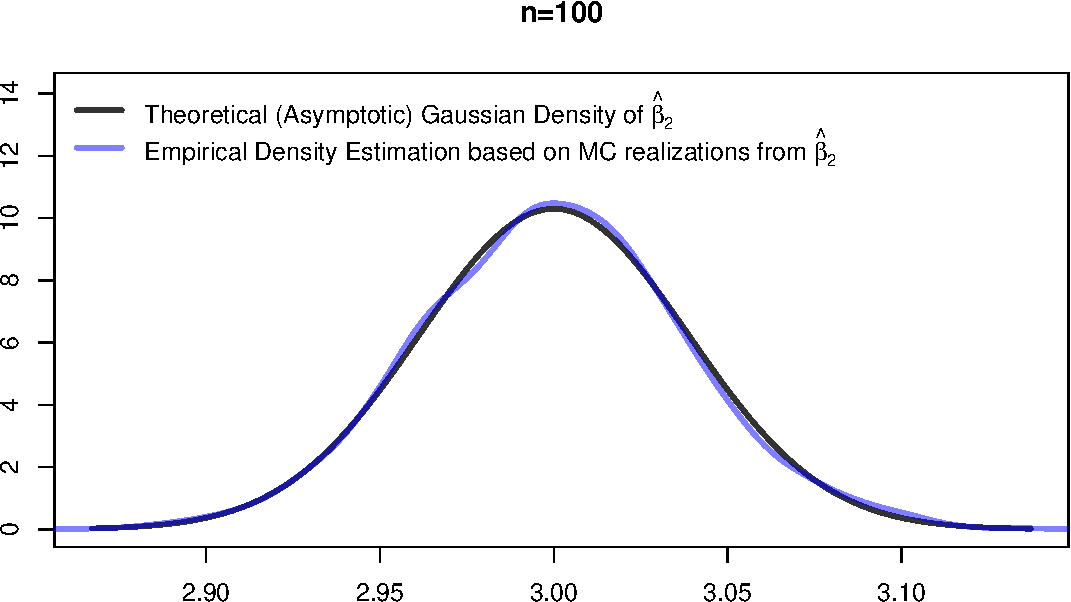
\includegraphics{./06-Asymptotics_files/figure-pdf/unnamed-chunk-5-1.pdf}

}

\end{figure}

Great! The nonparametric density estimation (estimated via
\texttt{density()}) computed from the \texttt{5000} simulated
realizations of \(\hat\beta_2\) is indicating that \(\hat\beta_2\) is
really normally distributed as described by our theoretical results in
Theorem~\ref{thm-OLSnormality1} (homoscedastic case) and in Equation
Equation~\ref{eq-OLSnormality1Rob} (heteroscedastic case).

However, is the asymptotic distribution of \(\hat\beta_2\) also usable
for (very) small samples like \(n=5\)? Let's check that:

\begin{Shaded}
\begin{Highlighting}[]
\FunctionTok{set.seed}\NormalTok{(}\DecValTok{123}\NormalTok{)}
\NormalTok{n           }\OtherTok{\textless{}{-}} \DecValTok{5}       \CommentTok{\# a small sample size}
\NormalTok{beta\_true   }\OtherTok{\textless{}{-}} \FunctionTok{c}\NormalTok{(}\DecValTok{2}\NormalTok{,}\DecValTok{3}\NormalTok{,}\DecValTok{4}\NormalTok{) }\CommentTok{\# true data vector}

\DocumentationTok{\#\# Mean and variance of the true asymptotic }
\DocumentationTok{\#\# normal distribution of beta\_hat\_2:}
\CommentTok{\# true mean}
\NormalTok{beta\_true\_2     }\OtherTok{\textless{}{-}}\NormalTok{ beta\_true[}\DecValTok{2}\NormalTok{] }
\CommentTok{\# true variance}
\NormalTok{var\_true\_beta\_2 }\OtherTok{\textless{}{-}}\NormalTok{ (}\FunctionTok{solve}\NormalTok{(}\FunctionTok{diag}\NormalTok{(}\FunctionTok{c}\NormalTok{(}\DecValTok{1}\NormalTok{, }\DecValTok{16}\SpecialCharTok{/}\DecValTok{3}\NormalTok{, }\DecValTok{25}\SpecialCharTok{/}\DecValTok{3}\NormalTok{)))}\SpecialCharTok{\%*\%} 
                          \FunctionTok{diag}\NormalTok{(}\FunctionTok{c}\NormalTok{(}\DecValTok{4}\SpecialCharTok{/}\DecValTok{9}\NormalTok{, }\DecValTok{64}\SpecialCharTok{/}\DecValTok{15}\NormalTok{, }\DecValTok{100}\SpecialCharTok{/}\DecValTok{27}\NormalTok{))}\SpecialCharTok{\%*\%} 
                    \FunctionTok{solve}\NormalTok{(}\FunctionTok{diag}\NormalTok{(}\FunctionTok{c}\NormalTok{(}\DecValTok{1}\NormalTok{, }\DecValTok{16}\SpecialCharTok{/}\DecValTok{3}\NormalTok{, }\DecValTok{25}\SpecialCharTok{/}\DecValTok{3}\NormalTok{))))[}\DecValTok{2}\NormalTok{,}\DecValTok{2}\NormalTok{]}\SpecialCharTok{/}\NormalTok{n}

\DocumentationTok{\#\# Let\textquotesingle{}s generate 5000 realizations from beta\_hat\_2, and check }
\DocumentationTok{\#\# whether their distribution is close to the true normal }
\DocumentationTok{\#\# distribution.}
\DocumentationTok{\#\# (We don\textquotesingle{}t condition on X since the theoretical limit }
\DocumentationTok{\#\# distribution is unconditional on X)}
\NormalTok{rep        }\OtherTok{\textless{}{-}} \DecValTok{5000} \CommentTok{\# MC replications}
\NormalTok{beta\_hat\_2 }\OtherTok{\textless{}{-}} \FunctionTok{rep}\NormalTok{(}\ConstantTok{NA}\NormalTok{, }\AttributeTok{times=}\NormalTok{rep)}
\DocumentationTok{\#\#}
\ControlFlowTok{for}\NormalTok{(r }\ControlFlowTok{in} \DecValTok{1}\SpecialCharTok{:}\NormalTok{rep)\{}
\NormalTok{    MC\_data }\OtherTok{\textless{}{-}} \FunctionTok{myDataGenerator}\NormalTok{(}\AttributeTok{n    =}\NormalTok{ n, }
                               \AttributeTok{beta =}\NormalTok{ beta\_true)}
\NormalTok{    lm\_obj        }\OtherTok{\textless{}{-}} \FunctionTok{lm}\NormalTok{(Y }\SpecialCharTok{\textasciitilde{}}\NormalTok{ X\_2 }\SpecialCharTok{+}\NormalTok{ X\_3, }\AttributeTok{data =}\NormalTok{ MC\_data)}
\NormalTok{    beta\_hat\_2[r] }\OtherTok{\textless{}{-}} \FunctionTok{coef}\NormalTok{(lm\_obj)[}\DecValTok{2}\NormalTok{]}
\NormalTok{\}}

\DocumentationTok{\#\# Compare:}
\DocumentationTok{\#\# True beta\_2 versus average of beta\_hat\_2 estimates}
\FunctionTok{c}\NormalTok{(beta\_true\_2, }\FunctionTok{round}\NormalTok{(}\FunctionTok{mean}\NormalTok{(beta\_hat\_2), }\DecValTok{4}\NormalTok{))}
\end{Highlighting}
\end{Shaded}

\begin{verbatim}
[1] 3.0000 2.9963
\end{verbatim}

OK, at least on average the \texttt{5000} simulated realizations of
\(\hat\beta_2\) are basically equal to the true mean
\(E(\hat\beta_2)=\beta_2=3\).

\begin{Shaded}
\begin{Highlighting}[]
\DocumentationTok{\#\# True variance of beta\_hat\_2 versus }
\DocumentationTok{\#\# empirical variance of beta\_hat\_2 estimates}
\FunctionTok{c}\NormalTok{(}\FunctionTok{round}\NormalTok{(var\_true\_beta\_2, }\DecValTok{4}\NormalTok{), }\FunctionTok{round}\NormalTok{(}\FunctionTok{var}\NormalTok{(beta\_hat\_2), }\DecValTok{4}\NormalTok{))}
\end{Highlighting}
\end{Shaded}

\begin{verbatim}
[1] 0.0300 0.0562
\end{verbatim}

Ouch! The theoretical large sample variance \(Var(\hat\beta_2)=0.03\) is
about 50\% smaller than the actual (small sample) variance of
\(\hat\beta_2\) approximated by the empirical variance of the
\texttt{5000} simulated realizations of \(\hat\beta_2\). That is, we
cannot simply use a large sample result in small samples.

\begin{Shaded}
\begin{Highlighting}[]
\DocumentationTok{\#\# True normal distribution of beta\_hat\_2 versus }
\DocumentationTok{\#\# empirical density of beta\_hat\_2 estimates}
\FunctionTok{library}\NormalTok{(}\StringTok{"scales"}\NormalTok{)}
\FunctionTok{curve}\NormalTok{(}\AttributeTok{expr =} \FunctionTok{dnorm}\NormalTok{(x, }\AttributeTok{mean =}\NormalTok{ beta\_true\_2, }
                   \AttributeTok{sd=}\FunctionTok{sqrt}\NormalTok{(var\_true\_beta\_2)), }
      \AttributeTok{xlab=}\StringTok{""}\NormalTok{,}\AttributeTok{ylab=}\StringTok{""}\NormalTok{, }\AttributeTok{col=}\FunctionTok{gray}\NormalTok{(.}\DecValTok{2}\NormalTok{), }\AttributeTok{lwd=}\DecValTok{3}\NormalTok{, }\AttributeTok{lty=}\DecValTok{1}\NormalTok{, }
\AttributeTok{xlim=}\FunctionTok{c}\NormalTok{(}\DecValTok{2}\NormalTok{,}\DecValTok{4}\NormalTok{), }\AttributeTok{ylim=}\FunctionTok{c}\NormalTok{(}\DecValTok{0}\NormalTok{,}\DecValTok{3}\NormalTok{),}\AttributeTok{main=}\FunctionTok{paste0}\NormalTok{(}\StringTok{"n="}\NormalTok{,n))}
\FunctionTok{lines}\NormalTok{(}\FunctionTok{density}\NormalTok{(beta\_hat\_2, }\AttributeTok{bw =} \FunctionTok{bw.SJ}\NormalTok{(beta\_hat\_2)), }
      \AttributeTok{col=}\FunctionTok{alpha}\NormalTok{(}\StringTok{"blue"}\NormalTok{,.}\DecValTok{5}\NormalTok{), }\AttributeTok{lwd=}\DecValTok{3}\NormalTok{)}
\FunctionTok{legend}\NormalTok{(}\StringTok{"topleft"}\NormalTok{, }\AttributeTok{lty=}\FunctionTok{c}\NormalTok{(}\DecValTok{1}\NormalTok{,}\DecValTok{1}\NormalTok{), }\AttributeTok{lwd=}\FunctionTok{c}\NormalTok{(}\DecValTok{3}\NormalTok{,}\DecValTok{3}\NormalTok{), }
     \AttributeTok{col=}\FunctionTok{c}\NormalTok{(}\FunctionTok{gray}\NormalTok{(.}\DecValTok{2}\NormalTok{), }\FunctionTok{alpha}\NormalTok{(}\StringTok{"blue"}\NormalTok{,.}\DecValTok{5}\NormalTok{)), }\AttributeTok{bty=}\StringTok{"n"}\NormalTok{, }\AttributeTok{legend=} 
\FunctionTok{c}\NormalTok{(}\FunctionTok{expression}\NormalTok{(}
  \StringTok{"Theoretical (Asymptotic) Gaussian Density of"}\SpecialCharTok{\textasciitilde{}}\FunctionTok{hat}\NormalTok{(beta)[}\DecValTok{2}\NormalTok{]), }
  \FunctionTok{expression}\NormalTok{(}
  \StringTok{"Empirical Density Estimation based on MC realizations from"}\SpecialCharTok{\textasciitilde{}}
  \FunctionTok{hat}\NormalTok{(beta)[}\DecValTok{2}\NormalTok{])))}
\end{Highlighting}
\end{Shaded}

\begin{figure}[H]

{\centering 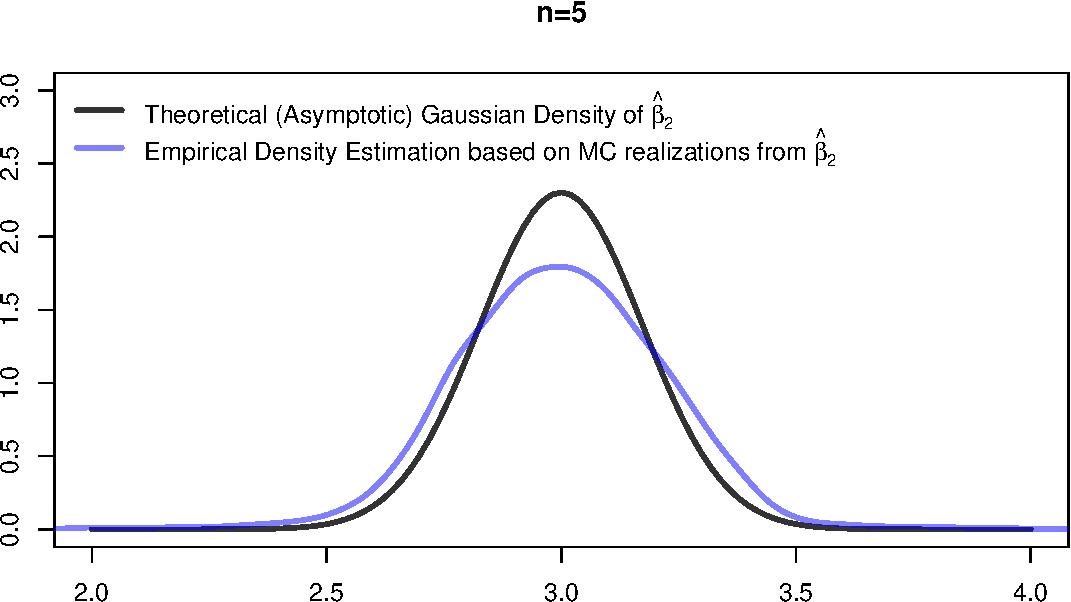
\includegraphics{./06-Asymptotics_files/figure-pdf/unnamed-chunk-8-1.pdf}

}

\end{figure}

Not good. The actual distribution has substantially fatter tails. That
is, if we would use the quantiles of the asymptotic distribution, we
would falsely reject the null-hypothesis too often (probability of type
I errors would be larger than the significance level).

\hypertarget{testing-multiple-and-single-parameters}{%
\subsection{Testing Multiple and Single
Parameters}\label{testing-multiple-and-single-parameters}}

In the following, we do inference about multiple parameters. We test the
(false) null hypothesis \begin{align*}
H_0:\;&\beta_2=3\quad\text{and}\quad\beta_3=5\\
\text{versus}\quad H_A:\;&\beta_2\neq 3\quad\text{and/or}\quad\beta_3\neq 5.
\end{align*} Or equivalently \begin{align*}
H_0:\;&R\beta -r = 0 \\
H_A:\;&R\beta -r \neq 0,
\end{align*} where

\[
R=\left(
\begin{matrix}
0&1&0\\
0&0&1\\
\end{matrix}\right)\quad\text{ and }\quad 
r=\left(\begin{matrix}3\\5\\\end{matrix}\right).
\]

The following \texttt{R} code can be used to test this hypothesis. Note
that we use HC3 robust variance estimation
\texttt{sandwich::vcovHC(lm\_obj,\ type="HC3")} to take into account
that the error terms are heteroscedastic.

\begin{Shaded}
\begin{Highlighting}[]
\FunctionTok{suppressMessages}\NormalTok{(}\FunctionTok{library}\NormalTok{(}\StringTok{"car"}\NormalTok{)) }\CommentTok{\# for linearHyothesis()}
\CommentTok{\# ?linearHypothesis}
\FunctionTok{library}\NormalTok{(}\StringTok{"sandwich"}\NormalTok{)}

\DocumentationTok{\#\# Generate data}
\NormalTok{MC\_data }\OtherTok{\textless{}{-}} \FunctionTok{myDataGenerator}\NormalTok{(}\AttributeTok{n    =} \DecValTok{100}\NormalTok{, }
                           \AttributeTok{beta =}\NormalTok{ beta\_true)}

\DocumentationTok{\#\# Estimate the linear regression model parameters}
\NormalTok{lm\_obj }\OtherTok{\textless{}{-}} \FunctionTok{lm}\NormalTok{(Y }\SpecialCharTok{\textasciitilde{}}\NormalTok{ X\_2 }\SpecialCharTok{+}\NormalTok{ X\_3, }\AttributeTok{data =}\NormalTok{ MC\_data)}

\NormalTok{vcovHC3\_mat }\OtherTok{\textless{}{-}}\NormalTok{ sandwich}\SpecialCharTok{::}\FunctionTok{vcovHC}\NormalTok{(lm\_obj, }\AttributeTok{type=}\StringTok{"HC3"}\NormalTok{)}

\DocumentationTok{\#\# Option 1:}
\NormalTok{car}\SpecialCharTok{::}\FunctionTok{linearHypothesis}\NormalTok{(}\AttributeTok{model =}\NormalTok{ lm\_obj, }
                      \AttributeTok{hypothesis.matrix =} \FunctionTok{c}\NormalTok{(}\StringTok{"X\_2=3"}\NormalTok{, }\StringTok{"X\_3=5"}\NormalTok{), }
                      \AttributeTok{vcov=}\NormalTok{vcovHC3\_mat)}
\end{Highlighting}
\end{Shaded}

\begin{verbatim}
Linear hypothesis test

Hypothesis:
X_2 = 3
X_3 = 5

Model 1: restricted model
Model 2: Y ~ X_2 + X_3

Note: Coefficient covariance matrix supplied.

  Res.Df Df      F    Pr(>F)    
1     99                        
2     97  2 1150.4 < 2.2e-16 ***
---
Signif. codes:  0 '***' 0.001 '**' 0.01 '*' 0.05 '.' 0.1 ' ' 1
\end{verbatim}

\begin{Shaded}
\begin{Highlighting}[]
\DocumentationTok{\#\# Option 2:}
\NormalTok{R }\OtherTok{\textless{}{-}} \FunctionTok{rbind}\NormalTok{(}\FunctionTok{c}\NormalTok{(}\DecValTok{0}\NormalTok{,}\DecValTok{1}\NormalTok{,}\DecValTok{0}\NormalTok{),}
           \FunctionTok{c}\NormalTok{(}\DecValTok{0}\NormalTok{,}\DecValTok{0}\NormalTok{,}\DecValTok{1}\NormalTok{))}
\NormalTok{car}\SpecialCharTok{::}\FunctionTok{linearHypothesis}\NormalTok{(}\AttributeTok{model =}\NormalTok{ lm\_obj, }
                      \AttributeTok{hypothesis.matrix =}\NormalTok{ R, }
                      \AttributeTok{rhs =} \FunctionTok{c}\NormalTok{(}\DecValTok{3}\NormalTok{,}\DecValTok{5}\NormalTok{),}
                      \AttributeTok{vcov=}\NormalTok{vcovHC3\_mat)}
\end{Highlighting}
\end{Shaded}

\begin{verbatim}
Linear hypothesis test

Hypothesis:
X_2 = 3
X_3 = 5

Model 1: restricted model
Model 2: Y ~ X_2 + X_3

Note: Coefficient covariance matrix supplied.

  Res.Df Df      F    Pr(>F)    
1     99                        
2     97  2 1150.4 < 2.2e-16 ***
---
Signif. codes:  0 '***' 0.001 '**' 0.01 '*' 0.05 '.' 0.1 ' ' 1
\end{verbatim}

The \(p\)-value is very small and allows us to reject the (false)
null-hypothesis at any of the usual significance levels.

Next, we do inference about a single parameter. We test \begin{align*}
H_0:&\beta_3=5\\
\text{versus}\quad H_A:&\beta_3\neq 5.
\end{align*}

\begin{Shaded}
\begin{Highlighting}[]
\CommentTok{\# Load libraries}
\FunctionTok{library}\NormalTok{(}\StringTok{"lmtest"}\NormalTok{)   }\CommentTok{\# for coeftest()}
\end{Highlighting}
\end{Shaded}

\begin{verbatim}
Loading required package: zoo
\end{verbatim}

\begin{verbatim}

Attaching package: 'zoo'
\end{verbatim}

\begin{verbatim}
The following objects are masked from 'package:base':

    as.Date, as.Date.numeric
\end{verbatim}

\begin{Shaded}
\begin{Highlighting}[]
\FunctionTok{library}\NormalTok{(}\StringTok{"sandwich"}\NormalTok{) }\CommentTok{\# for vcovHC()}

\DocumentationTok{\#\# Generate data}
\NormalTok{n }\OtherTok{\textless{}{-}} \DecValTok{100}
\NormalTok{MC\_data }\OtherTok{\textless{}{-}} \FunctionTok{myDataGenerator}\NormalTok{(}\AttributeTok{n    =}\NormalTok{ n, }
                           \AttributeTok{beta =}\NormalTok{ beta\_true)}

\DocumentationTok{\#\# Estimate the linear regression model parameters}
\NormalTok{lm\_obj }\OtherTok{\textless{}{-}} \FunctionTok{lm}\NormalTok{(Y }\SpecialCharTok{\textasciitilde{}}\NormalTok{ X\_2 }\SpecialCharTok{+}\NormalTok{ X\_3, }\AttributeTok{data =}\NormalTok{ MC\_data)}

\DocumentationTok{\#\# Robust t test}

\DocumentationTok{\#\# Robust standard error for \textbackslash{}hat\{\textbackslash{}beta\}\_3:}
\NormalTok{SE\_rob }\OtherTok{\textless{}{-}} \FunctionTok{sqrt}\NormalTok{(}\FunctionTok{vcovHC}\NormalTok{(lm\_obj, }\AttributeTok{type =} \StringTok{"HC3"}\NormalTok{)[}\DecValTok{3}\NormalTok{,}\DecValTok{3}\NormalTok{])}
\DocumentationTok{\#\# hypothetical (H0) value of \textbackslash{}beta\_3:}
\NormalTok{beta\_3\_H0 }\OtherTok{\textless{}{-}} \DecValTok{5}
\DocumentationTok{\#\# estimate for beta\_3:}
\NormalTok{beta\_3\_hat }\OtherTok{\textless{}{-}} \FunctionTok{coef}\NormalTok{(lm\_obj)[}\DecValTok{3}\NormalTok{]}
\DocumentationTok{\#\# robust t{-}test statistic}
\NormalTok{t\_test\_stat }\OtherTok{\textless{}{-}}\NormalTok{ (beta\_3\_hat }\SpecialCharTok{{-}}\NormalTok{ beta\_3\_H0)}\SpecialCharTok{/}\NormalTok{SE\_rob}
\DocumentationTok{\#\# p{-}value}
\NormalTok{K }\OtherTok{\textless{}{-}} \FunctionTok{length}\NormalTok{(}\FunctionTok{coef}\NormalTok{(lm\_obj))}
\DocumentationTok{\#\#}
\NormalTok{p\_value }\OtherTok{\textless{}{-}} \DecValTok{2} \SpecialCharTok{*} \FunctionTok{min}\NormalTok{(   }\FunctionTok{pt}\NormalTok{(}\AttributeTok{q =}\NormalTok{ t\_test\_stat, }\AttributeTok{df =}\NormalTok{ n }\SpecialCharTok{{-}}\NormalTok{ K), }
                   \DecValTok{1}\SpecialCharTok{{-}} \FunctionTok{pt}\NormalTok{(}\AttributeTok{q =}\NormalTok{ t\_test\_stat, }\AttributeTok{df =}\NormalTok{ n }\SpecialCharTok{{-}}\NormalTok{ K))}
\NormalTok{p\_value}
\end{Highlighting}
\end{Shaded}

\begin{verbatim}
[1] 4.330845e-65
\end{verbatim}

Again, the \(p\)-value is very small and allows us to reject the (false)
null-hypothesis at any of the usual significance levels.

\bookmarksetup{startatroot}

\hypertarget{references-2}{%
\chapter*{References}\label{references-2}}
\addcontentsline{toc}{chapter}{References}

\bookmarksetup{startatroot}

\hypertarget{ivr}{%
\chapter{Instrumental Variables Regression}\label{ivr}}

The current version of this chapter is basically completly taken from
the free online book: \url{www.econometrics-with-r.org} (Hanck et al.
2021)

\bigskip

Regression models may suffer from problems like omitted variables,
measurement errors and simultaneous causality. If so, the error term
\(\eps_i\) is correlated with the regressor, \(X_{ik}\) say, and the
corresponding coefficient of interest, \(\beta_k\), is estimated
\textbf{inconsistently}. If one is lucky, one can add, for instance, the
omitted variables to the regression to mitigate the risk of biased
estimations (\say{omitted variables bias}). However, if omitted
variables cannot be measured or are not available for other reasons,
multiple regression cannot solve the problem. The same issue arises if
there is \say{simultaneous causality}. When causality runs from \(X\) to
\(Y\) \emph{and vice versa} (e.g.~if
\(Y=\text{Demanded quantity of a good}\) and
\(X=\text{Price of this good}\)), there will be an estimation bias that
cannot be corrected for by multiple regression.

A general technique for obtaining a consistent estimator of the
coefficient of interest is instrumental variables (IV) regression. In
this chapter we focus on the IV regression tool called \emph{two-stage
least squares} (TSLS). The first sections briefly recap the general
mechanics and assumptions of IV regression and show how to perform TSLS
estimation using \textsf{R}. Next, IV regression is used for estimating
the elasticity of the demand for cigarettes --- a classical example
where multiple regression fails to do the job because of simultaneous
causality.

\hypertarget{TIVEWASRAASI}{%
\section{The IV Estimator with a Single Regressor and a Single
Instrument}\label{TIVEWASRAASI}}

Consider the simple regression model \begin{align}
  Y_i = \beta_1 + \beta_2 X_i + \eps_i \ \ , \ \ i=1,\dots,n, \label{eq:srm12}
\end{align} where the error term \(\eps_i\) is correlated with the
regressor \(X_i\) (\(X\) is the called \say{\textit{endogenous}}). In
this case Assumption 2 is violated, that is, strict exogeneity and
orthogonality between \(X_i\) and \(\eps_i\) do not hold. Therefore, OLS
estimation (also maximum likelihood and methods of moments estimation)
is inconsistent for the true \(\beta_2\). In the most simple case, IV
regression uses a single instrumental variable \(Z_i\) to obtain a
consistent estimator for \(\beta_2\).

\paragraph*{Conditions for valid instruments:}

\(Z_i\) must satisfy two conditions to be a valid instrument:

\begin{enumerate}
\item \textbf{Instrument relevance condition:}\\
$X_i$ and its instrument $Z_i$ \emph{must be} correlated: $\rho_{Z,X} \neq 0$.
\item \textbf{Instrument exogeneity condition:}\\
$E(\eps_i|Z_i)=0$. As a consequence: The instrument $Z_i$ \emph{must not be} correlated with the error term $\eps_i$: $\rho_{Z,\eps} = 0$.
\end{enumerate}

\hypertarget{the-two-stage-least-squares-estimator}{%
\subsection{The Two-Stage Least Squares
Estimator}\label{the-two-stage-least-squares-estimator}}

As can be guessed from its name, TSLS proceeds in two stages. In the
first stage, the variation in the endogenous regressor \(X_i\) is
decomposed into a \say{problem-free} component that is explained by the
(exogenous) instrument \(Z_i\) and a problematic component that is
correlated with the error \(\eps_i\). The second stage uses the
problem-free component of the variation in \(X_i\) to estimate
\(\beta_2\).

The first stage regression model is

\[
X_i = \pi_0 + \pi_1 Z_i + \nu_i,
\]

where \(\pi_0 + \pi_1 Z_i\) is the component of \(X_i\) that is
explained by \(Z_i\) while \(\nu_i\) is the component (an error term)
that cannot be explained by \(Z_i\) and exhibits correlation with
\(\eps_i\).

Using the OLS estimates \(\widehat{\pi}_0\) and \(\widehat{\pi}_1\) we
obtain predicted values
\(\widehat{X}_i=\hat\pi_0+\hat\pi_1 Z_i,\ i=1,\dots,n\). If \(Z_i\) is a
valid instrument, the \(\widehat{X}_i\) are problem-free in the sense
that \(\widehat{X}_i\) is \textbf{exogenous} in a regression of \(Y_i\)
on \(\widehat{X}_i\) which is done in the second stage regression. The
second stage produces \(\widehat{\beta}_1^{TSLS}\) and
\(\widehat{\beta}_2^{TSLS}\), the TSLS estimates of \(\beta_1\) and
\(\beta_2\).

For the case of a single instrument one can show that the TSLS estimator
of \(\beta_2\) is \begin{align}
\widehat{\beta}_2^{TSLS} = \frac{s_{ZY}}{s_{ZX}} = \frac{\frac{1}{n-1}\sum_{i=1}^n(Y_i - \overline{Y})(Z_i - \overline{Z})}{\frac{1}{n-1}\sum_{i=1}^n(X_i - \overline{X})(Z_i - \overline{Z})}, \label{eq:simpletsls}
\end{align} which is nothing but the ratio of the sample covariance
between \(Z_i\) and \(Y_i\) to the sample covariance between \(Z_i\) and
\(X_i\).

The estimator in \eqref{eq:simpletsls} is a consistent estimator for
\(\beta_2\) in \eqref{eq:srm12} under the assumption that \(Z_i\) is a
valid instrument. The CLT implies that the distribution of
\(\widehat{\beta}_2^{TSLS}\) can be approximated by a normal
distribution if the sample size \(n\) is large. This allows us to use
\(t\)-statistics, \(F\)-statistics, confidence intervals, etc.

\hypertarget{application-demand-for-cigarettes-12}{%
\subsection{Application: Demand For Cigarettes
(1/2)}\label{application-demand-for-cigarettes-12}}

The relation between the demand for and the price of commodities is a
simple yet widespread problem in economics. Health economics is
concerned with the study of how health-affecting behavior of individuals
is influenced by the health-care system and regulation policy. Probably
the most prominent example in public policy debates is smoking as it is
related to many illnesses and negative externalities.

It is plausible that cigarette consumption can be reduced by taxing
cigarettes more heavily. The question is by \emph{how much} taxes must
be increased to reach a certain reduction in cigarette consumption.
Economists use elasticities to answer this kind of question. Since the
price elasticity for the demand of cigarettes is unknown, it must be
estimated. A simple OLS regression of log quantity on log price cannot
be used to estimate the effect of interest since there is simultaneous
causality between demand and supply. Instead, IV regression can be used.

We use the data set \texttt{CigarettesSW} which comes with the package
\texttt{AER}. It is a panel data set that contains observations on
cigarette consumption and several economic indicators for all 48
continental federal states of the U.S. from 1985 to 1995. In the
following, however, we consider data for the cross section of states in
1995 only -- that is, we transform the panel data to a cross-sectional
data set. We start by loading the package, attaching the data set. An
overview about summary statistics for each of the variables is returned
by \texttt{summary(CigarettesSW)}. Use \texttt{?CigarettesSW} for a
detailed description of the variables.

\begin{Shaded}
\begin{Highlighting}[]
\CommentTok{\# load the data set and get an overview}
\FunctionTok{library}\NormalTok{(}\StringTok{"AER"}\NormalTok{)}
\FunctionTok{data}\NormalTok{(}\StringTok{"CigarettesSW"}\NormalTok{)}
\FunctionTok{summary}\NormalTok{(CigarettesSW)}
\end{Highlighting}
\end{Shaded}

\begin{verbatim}
     state      year         cpi          population           packs       
 AL     : 2   1985:48   Min.   :1.076   Min.   :  478447   Min.   : 49.27  
 AR     : 2   1995:48   1st Qu.:1.076   1st Qu.: 1622606   1st Qu.: 92.45  
 AZ     : 2             Median :1.300   Median : 3697472   Median :110.16  
 CA     : 2             Mean   :1.300   Mean   : 5168866   Mean   :109.18  
 CO     : 2             3rd Qu.:1.524   3rd Qu.: 5901500   3rd Qu.:123.52  
 CT     : 2             Max.   :1.524   Max.   :31493524   Max.   :197.99  
 (Other):84                                                                
     income               tax            price             taxs       
 Min.   :  6887097   Min.   :18.00   Min.   : 84.97   Min.   : 21.27  
 1st Qu.: 25520384   1st Qu.:31.00   1st Qu.:102.71   1st Qu.: 34.77  
 Median : 61661644   Median :37.00   Median :137.72   Median : 41.05  
 Mean   : 99878736   Mean   :42.68   Mean   :143.45   Mean   : 48.33  
 3rd Qu.:127313964   3rd Qu.:50.88   3rd Qu.:176.15   3rd Qu.: 59.48  
 Max.   :771470144   Max.   :99.00   Max.   :240.85   Max.   :112.63  
                                                                      
\end{verbatim}

We are interested in estimating \(\beta_2\) in \begin{align}
  \log(Q_i^{cigarettes}) = \beta_1 + \beta_2 \log(P_i^{cigarettes}) + \eps_i, \label{eq:cigstsls}
\end{align} where \(Q_i^{cigarettes}\) is the number of cigarette packs
per capita sold and \(P_i^{cigarettes}\) is the after-tax average real
price per pack of cigarettes in state \(i=1,\dots,n=48\).

The instrumental variable we are going to use for instrumenting the
endogenous regressor \(\log(P_i^{cigarettes})\) is \(SalesTax\), the
portion of taxes on cigarettes arising from the general sales tax.
\(SalesTax\) is measured in dollars per pack. The idea is that:

\begin{enumerate}
\item $SalesTax$ is a relevant instrument as it is included in the after-tax average price per pack. 
\item Also, it is plausible that $SalesTax$ is exogenous since the sales tax does not influence quantity sold directly but indirectly through the price.
\end{enumerate}

In the following, we perform some transformations in order to obtain
deflated cross section data for the year 1995. We also compute the
sample correlation between the sales tax and price per pack. The sample
correlation is a consistent estimator of the population correlation. The
estimate of approximately \(0.614\) indicates that \(SalesTax\) and
\(P_i^{cigarettes}\) exhibit positive correlation which meets our
expectations: higher sales taxes lead to higher prices. However, a
correlation analysis like this is not sufficient for checking whether
the instrument is relevant. We will later come back to the issue of
checking whether an instrument is relevant and exogenous; see Chapter
@ref(civ).

\begin{Shaded}
\begin{Highlighting}[]
\CommentTok{\# compute real per capita prices}
\NormalTok{CigarettesSW}\SpecialCharTok{$}\NormalTok{rprice }\OtherTok{\textless{}{-}} \FunctionTok{with}\NormalTok{(CigarettesSW, price }\SpecialCharTok{/}\NormalTok{ cpi)}

\CommentTok{\#  compute the sales tax}
\NormalTok{CigarettesSW}\SpecialCharTok{$}\NormalTok{salestax }\OtherTok{\textless{}{-}} \FunctionTok{with}\NormalTok{(CigarettesSW, (taxs }\SpecialCharTok{{-}}\NormalTok{ tax) }\SpecialCharTok{/}\NormalTok{ cpi)}

\CommentTok{\# check the correlation between sales tax and price}
\FunctionTok{cor}\NormalTok{(CigarettesSW}\SpecialCharTok{$}\NormalTok{salestax, CigarettesSW}\SpecialCharTok{$}\NormalTok{price)}
\end{Highlighting}
\end{Shaded}

\begin{verbatim}
[1] 0.6141228
\end{verbatim}

\begin{Shaded}
\begin{Highlighting}[]
\CommentTok{\# generate a subset for the year 1995}
\NormalTok{c1995 }\OtherTok{\textless{}{-}} \FunctionTok{subset}\NormalTok{(CigarettesSW, year }\SpecialCharTok{==} \StringTok{"1995"}\NormalTok{)}
\end{Highlighting}
\end{Shaded}

The first stage regression is

\[
\log(P_i^{cigarettes}) = \pi_0 + \pi_1 SalesTax_i + \nu_i.
\]

We estimate this model in \textsf{R} using \texttt{lm()}. In the second
stage we run a regression of \(\log(Q_i^{cigarettes})\) on
\(\widehat{\log(P_i^{cigarettes})}\) to obtain
\(\widehat{\beta}_1^{TSLS}\) and \(\widehat{\beta}_2^{TSLS}\).

\begin{Shaded}
\begin{Highlighting}[]
\CommentTok{\# perform the first stage regression}
\NormalTok{cig\_s1 }\OtherTok{\textless{}{-}} \FunctionTok{lm}\NormalTok{(}\FunctionTok{log}\NormalTok{(rprice) }\SpecialCharTok{\textasciitilde{}}\NormalTok{ salestax, }\AttributeTok{data =}\NormalTok{ c1995)}

\FunctionTok{coeftest}\NormalTok{(cig\_s1, }\AttributeTok{vcov =}\NormalTok{ vcovHC, }\AttributeTok{type =} \StringTok{"HC1"}\NormalTok{)}
\end{Highlighting}
\end{Shaded}

\begin{verbatim}

t test of coefficients:

             Estimate Std. Error  t value  Pr(>|t|)    
(Intercept) 4.6165463  0.0289177 159.6444 < 2.2e-16 ***
salestax    0.0307289  0.0048354   6.3549 8.489e-08 ***
---
Signif. codes:  0 '***' 0.001 '**' 0.01 '*' 0.05 '.' 0.1 ' ' 1
\end{verbatim}

The first stage regression is

\[
\widehat{\log(P_i^{cigarettes})} = \underset{(0.03)}{4.62} + \underset{(0.005)}{0.031}\; SalesTax_i
\]

which predicts the relation between sales tax price per cigarettes to be
positive. How much of the observed variation in \(\log(P^{cigarettes})\)
is explained by the instrument \(SalesTax\)? This can be answered by
looking at the regression's \(R^2\) which states that about \(47\%\) of
the variation in after tax prices is explained by the variation of the
sales tax across states.

\begin{Shaded}
\begin{Highlighting}[]
\CommentTok{\# inspect the R\^{}2 of the first stage regression}
\FunctionTok{summary}\NormalTok{(cig\_s1)}\SpecialCharTok{$}\NormalTok{r.squared}
\end{Highlighting}
\end{Shaded}

\begin{verbatim}
[1] 0.4709961
\end{verbatim}

We next store \(\widehat{\log(P_i^{cigarettes})}\), the fitted values
obtained by the first stage regression \texttt{cig\_s1}, in the variable
\texttt{lcigp\_pred}.

\begin{Shaded}
\begin{Highlighting}[]
\CommentTok{\# store the predicted values}
\NormalTok{lcigp\_pred }\OtherTok{\textless{}{-}}\NormalTok{ cig\_s1}\SpecialCharTok{$}\NormalTok{fitted.values}
\end{Highlighting}
\end{Shaded}

Next, we run the second stage regression which gives us the TSLS
estimates we seek.

\begin{Shaded}
\begin{Highlighting}[]
\CommentTok{\# run the stage 2 regression}
\NormalTok{cig\_s2 }\OtherTok{\textless{}{-}} \FunctionTok{lm}\NormalTok{(}\FunctionTok{log}\NormalTok{(c1995}\SpecialCharTok{$}\NormalTok{packs) }\SpecialCharTok{\textasciitilde{}}\NormalTok{ lcigp\_pred)}
\FunctionTok{coeftest}\NormalTok{(cig\_s2, }\AttributeTok{vcov =}\NormalTok{ vcovHC, }\AttributeTok{type =} \StringTok{"HC1"}\NormalTok{)}
\end{Highlighting}
\end{Shaded}

\begin{verbatim}

t test of coefficients:

            Estimate Std. Error t value  Pr(>|t|)    
(Intercept)   9.7199     1.5971  6.0859 2.153e-07 ***
lcigp_pred   -1.0836     0.3337 -3.2472  0.002178 ** 
---
Signif. codes:  0 '***' 0.001 '**' 0.01 '*' 0.05 '.' 0.1 ' ' 1
\end{verbatim}

Thus estimating the model \eqref{eq:cigstsls} using TSLS yields
\begin{align}
  \widehat{\log(Q_i^{cigarettes})} = \underset{(1.60)}{9.72} - \underset{(0.33)}{1.08} \widehat{\log(P_i^{cigarettes})}, \label{eq:ecigstsls}
\end{align}

The function \texttt{ivreg()} from the package \texttt{AER} carries out
TSLS procedure automatically. It is used similarly as \texttt{lm()}.
Instruments can be added to the usual specification of the regression
formula using a vertical bar separating the model equation from the
instruments. Thus, for the regression at hand the correct formula is
\texttt{log(packs)\ \textasciitilde{}\ log(rprice)\ \textbar{}\ salestax}.

\begin{Shaded}
\begin{Highlighting}[]
\CommentTok{\# perform TSLS using \textquotesingle{}ivreg()\textquotesingle{}}
\NormalTok{cig\_ivreg }\OtherTok{\textless{}{-}} \FunctionTok{ivreg}\NormalTok{(}\FunctionTok{log}\NormalTok{(packs) }\SpecialCharTok{\textasciitilde{}} \FunctionTok{log}\NormalTok{(rprice) }\SpecialCharTok{|}\NormalTok{ salestax, }
                   \AttributeTok{data =}\NormalTok{ c1995)}

\FunctionTok{coeftest}\NormalTok{(cig\_ivreg, }\AttributeTok{vcov =}\NormalTok{ vcovHC, }\AttributeTok{type =} \StringTok{"HC1"}\NormalTok{)}
\end{Highlighting}
\end{Shaded}

\begin{verbatim}

t test of coefficients:

            Estimate Std. Error t value  Pr(>|t|)    
(Intercept)  9.71988    1.52832  6.3598 8.346e-08 ***
log(rprice) -1.08359    0.31892 -3.3977  0.001411 ** 
---
Signif. codes:  0 '***' 0.001 '**' 0.01 '*' 0.05 '.' 0.1 ' ' 1
\end{verbatim}

We find that the coefficient estimates coincide for both approaches.

\paragraph*{Two Notes on the Computation of TSLS Standard Errors:}
\begin{enumerate}
\item We have demonstrated that running the individual regressions for each stage of TSLS using `lm()` leads to the same coefficient estimates as when using `ivreg()`. However, the standard errors reported for the second-stage regression, e.g., by `coeftest()` or `summary()`, are \textbf{invalid}: neither adjusts for using predictions from the first-stage regression as regressors in the second-stage regression. Fortunately, `ivreg()` performs the necessary adjustment automatically. This is another advantage over manual step-by-step estimation which we have done above for demonstrating the mechanics of the procedure.
\item Just like in multiple regression it is important to compute heteroskedasticity-robust standard errors as we have done above using `vcovHC()`.
\end{enumerate}

The TSLS estimate for \(\beta_2\) in \eqref{eq:ecigstsls} suggests that
an increase in cigarette prices by one percent reduces cigarette
consumption by roughly \(1.08\) percentage points, which is fairly
elastic. However, we should keep in mind that this estimate might not be
trustworthy even though we used IV estimation: there still might be a
bias due to \textbf{omitted variables}. Thus a multiple IV regression
approach is needed to reduce the risk of omitted variable biases.

\hypertarget{TGIVRM}{%
\section{The General IV Regression Model}\label{TGIVRM}}

The simple IV regression model is easily extended to a multiple
regression model which we refer to as the general IV regression model.
In this model we distinguish between four types of variables: the
dependent variable, included exogenous variables, included endogenous
variables and instrumental variables: \begin{align}
  Y_i = \beta_1 + \beta_2 X_{2i} + \dots + \beta_K X_{Ki} + \beta_{K+1} W_{1i} + \dots + \beta_{K+r} W_{ri} + \eps_i, \label{eq:givmodel}
\end{align} with \(i=1,\dots,n\) is the general instrumental variables
regression model where

\begin{itemize}
\item $Y_i$ is the dependent variable
\item $\beta_1,\dots,\beta_{K+r}$ are $K+r$ unknown regression coefficients
\item $X_{2i},\dots,X_{Ki}$ are $K-1$ endogenous regressors 
\item $W_{1i},\dots,W_{ri}$ are $r$ exogenous regressors which are uncorrelated with $\eps_i$
\item $\eps_i$ is the error term
\item $Z_{1i},\dots,Z_{mi}$ are $m$ instrumental variables
\end{itemize}
\vspace{0.5cm}

The coefficients are \textbf{overidentified} if \(m>(K-1)\). If
\(m<(K-1)\), the coefficients are \textbf{underidentified} and when
\(m=(K-1)\) they are \textbf{exactly identified}. For estimation of the
IV regression model we require exact identification or
overidentification.

Estimating regression models with TSLS using multiple instruments by
means of \texttt{ivreg()} is straightforward. There are, however, some
subtleties in correctly specifying the regression formula. Assume that
you want to estimate the model

\[
Y_i = \beta_1 + \beta_2 X_{2i} + \beta_3 X_{3i} + \beta_4 W_{1i} + \eps_i
\]

where \(X_{2i}\) and \(X_{3i}\) are endogenous regressors that shall be
instrumented by \(Z_{1i}\), \(Z_{2i}\) and \(Z_{3i}\), and where
\(W_{1i}\) is an exogenous regressor. Say the corresponding data is
available in a \texttt{data.frame} with column names \texttt{y},
\texttt{x2}, \texttt{x3}, \texttt{w1}, \texttt{z1}, \texttt{z2} and
\texttt{z3}. It might be tempting to specify the argument
\texttt{formula} in your call of \texttt{ivreg()} as
\texttt{y\ \textasciitilde{}\ x2\ +\ x3\ +\ w1\ \textbar{}\ z1\ +\ z2\ +\ z3}
which is, however, \textbf{wrong}. As explained in the documentation of
\texttt{ivreg()} (see \texttt{?ivreg}), it is necessary to list
\emph{all} exogenous variables as instruments too, that is joining them
by \texttt{+}'s on the right of the vertical bar:
\texttt{y\ \textasciitilde{}\ x2\ +\ x3\ +\ w1\ \textbar{}\ w1\ +\ z1\ +\ z2\ +\ z3},
where \texttt{w1} is ``instrumenting itself''.

Similarly to the simple IV regression model, the general IV model
\eqref{eq:givmodel} can be estimated using the two-stage least squares
estimator:

\begin{itemize}
\item \textbf{First-stage regression(s):}\\
Run an OLS regression for each of the endogenous variables ($X_{2i},\dots,X_{Ki}$) on all instrumental variables ($Z_{1i},\dots,Z_{mi}$), all exogenous variables ($W_{1i},\dots,W_{ri}$) \textbf{and an intercept}. Compute the fitted values ($\widehat{X}_{2i},\dots,\widehat{X}_{Ki}$).
\item \textbf{Second-stage regression:}\\
Regress the dependent variable on the predicted values of all endogenous regressors, all exogenous variables and an intercept using OLS. This gives $\widehat{\beta}_{1}^{TSLS},\dots,\widehat{\beta}_{K+r}^{TSLS}$, the TSLS estimates of the model coefficients.
\end{itemize}

In the general IV regression model, the instrument relevance and
instrument exogeneity assumptions are equivalent to the case of the
simple regression model with a single endogenous regressor and only one
instrument. That is, for \(Z_{1i},\dots,Z_{mi}\) to be a set of valid
instruments, the following two conditions must be fulfilled:

\begin{enumerate}
\item \textbf{Instrument Relevance}\\
If there are $K-1$ endogenous variables, $r$ exogenous variables and $m\geq K-1$ instruments and the $\widehat{X}_{2i}^*,\dots,\widehat{X}_{Ki}^*$ are the predicted values from the $K-1$ population first stage regressions, it must hold that $$(\widehat{X}_{2i}^*,\dots,\widehat{X}_{Ki}^*, W_{1i}, \dots, W_{ri},1)$$ are not perfectly multicollinear, where \say{$1$} denotes the constant regressor (intercept) which equals $1$ for all observations.\\
\textit{Explanations}:  Let's say there is only one endogenous regressor $X_i$. If all the instruments $Z_{1i},\dots,Z_{mi}$ are irrelevant, all the $\widehat{X}^*_i$ are just the mean of $X$ such that there is perfect multicollinearity with the constant intercept $1$.\\
\item \textbf{Instrument Exogeneity}\\
$E(\eps_i|Z_{1i},\dots,Z_{im})=0$. Consequently, all $m$ instruments must be uncorrelated with the error term, 


$$
\rho_{Z_{1},\eps} = 0,\dots,\rho_{Z_{m},\eps} = 0.
$$


\end{enumerate}

One can show that if the IV regression assumptions hold, the TSLS
estimator in \eqref{eq:givmodel} is consistent and normally distributed
when the sample size \(n\) is large. That is, if we have valid
instruments, we obtain valid statistical inference using \(t\)-tests,
\(F\)-tests and confidence intervals for the model coefficients.

\hypertarget{application-demand-for-cigarettes-22}{%
\subsection{Application: Demand for Cigarettes
(2/2)}\label{application-demand-for-cigarettes-22}}

The estimated elasticity of the demand for cigarettes in
\eqref{eq:srm12} is \(1.08\). Although \eqref{eq:srm12} was estimated
using IV regression it is plausible that this IV estimate is biased. The
TSLS estimator is inconsistent for the true \(\beta_2\) if the
instrument (here: the real sales tax per pack) is invalid, i.e., if the
instrument correlates with the error term. This is likely to be the case
here since there are economic factors, like state income, which impact
the demand for cigarettes and correlate with the sales tax. States with
high personal income tend to generate tax revenues by income taxes and
less by sales taxes. Consequently, state income should be included in
the regression model. \begin{align}
  \log(Q_i^{cigarettes}) = \beta_1 + \beta_2 \log(P_i^{cigarettes}) + \beta_3 \log(income_i) + \eps_i \label{eq:mcigstsls1}
\end{align}

Before estimating \eqref{eq:mcigstsls1} using \texttt{ivreg()} we define
\(income\) as real per capita income \texttt{rincome} and append it to
the data set \texttt{CigarettesSW}.

\begin{Shaded}
\begin{Highlighting}[]
\CommentTok{\# add real income to the dataset (cpi: consumer price index)}
\NormalTok{CigarettesSW}\SpecialCharTok{$}\NormalTok{rincome }\OtherTok{\textless{}{-}} \FunctionTok{with}\NormalTok{(CigarettesSW, }
\NormalTok{                             income }\SpecialCharTok{/}\NormalTok{ population }\SpecialCharTok{/}\NormalTok{ cpi)}

\NormalTok{c1995 }\OtherTok{\textless{}{-}} \FunctionTok{subset}\NormalTok{(CigarettesSW, year }\SpecialCharTok{==} \StringTok{"1995"}\NormalTok{)}
\end{Highlighting}
\end{Shaded}

\begin{Shaded}
\begin{Highlighting}[]
\CommentTok{\# estimate the model}
\NormalTok{cig\_ivreg2 }\OtherTok{\textless{}{-}} \FunctionTok{ivreg}\NormalTok{(}\FunctionTok{log}\NormalTok{(packs) }\SpecialCharTok{\textasciitilde{}} \FunctionTok{log}\NormalTok{(rprice) }\SpecialCharTok{+} 
                                 \FunctionTok{log}\NormalTok{(rincome) }\SpecialCharTok{|} \FunctionTok{log}\NormalTok{(rincome) }\SpecialCharTok{+} 
\NormalTok{                    salestax, }\AttributeTok{data =}\NormalTok{ c1995)}

\FunctionTok{coeftest}\NormalTok{(cig\_ivreg2, }\AttributeTok{vcov =}\NormalTok{ vcovHC, }\AttributeTok{type =} \StringTok{"HC1"}\NormalTok{)}
\end{Highlighting}
\end{Shaded}

\begin{verbatim}

t test of coefficients:

             Estimate Std. Error t value  Pr(>|t|)    
(Intercept)   9.43066    1.25939  7.4883 1.935e-09 ***
log(rprice)  -1.14338    0.37230 -3.0711  0.003611 ** 
log(rincome)  0.21452    0.31175  0.6881  0.494917    
---
Signif. codes:  0 '***' 0.001 '**' 0.01 '*' 0.05 '.' 0.1 ' ' 1
\end{verbatim}

We obtain \begin{align}
  \widehat{\log(Q_i^{cigarettes})} = \underset{(1.26)}{9.42} - \underset{(0.37)}{1.14} \log(P_i^{cigarettes}) + \underset{(0.31)}{0.21} \log(income_i). \label{eq:emcigstsls2}
\end{align}

In the following we add the cigarette-specific taxes (\(cigtax_i\)) as a
further instrumental variable and estimate again using TSLS.

\begin{Shaded}
\begin{Highlighting}[]
\CommentTok{\# add cigtax to the data set}
\NormalTok{CigarettesSW}\SpecialCharTok{$}\NormalTok{cigtax }\OtherTok{\textless{}{-}} \FunctionTok{with}\NormalTok{(CigarettesSW, tax}\SpecialCharTok{/}\NormalTok{cpi)}

\NormalTok{c1995 }\OtherTok{\textless{}{-}} \FunctionTok{subset}\NormalTok{(CigarettesSW, year }\SpecialCharTok{==} \StringTok{"1995"}\NormalTok{)}
\end{Highlighting}
\end{Shaded}

\begin{Shaded}
\begin{Highlighting}[]
\CommentTok{\# estimate the model}
\NormalTok{cig\_ivreg3 }\OtherTok{\textless{}{-}} \FunctionTok{ivreg}\NormalTok{(}\FunctionTok{log}\NormalTok{(packs) }\SpecialCharTok{\textasciitilde{}} \FunctionTok{log}\NormalTok{(rprice) }\SpecialCharTok{+} \FunctionTok{log}\NormalTok{(rincome) }\SpecialCharTok{|} 
                    \FunctionTok{log}\NormalTok{(rincome) }\SpecialCharTok{+}\NormalTok{ salestax }\SpecialCharTok{+}\NormalTok{ cigtax, }
                    \AttributeTok{data =}\NormalTok{ c1995)}

\FunctionTok{coeftest}\NormalTok{(cig\_ivreg3, }\AttributeTok{vcov =}\NormalTok{ vcovHC, }\AttributeTok{type =} \StringTok{"HC1"}\NormalTok{)}
\end{Highlighting}
\end{Shaded}

\begin{verbatim}

t test of coefficients:

             Estimate Std. Error t value  Pr(>|t|)    
(Intercept)   9.89496    0.95922 10.3157 1.947e-13 ***
log(rprice)  -1.27742    0.24961 -5.1177 6.211e-06 ***
log(rincome)  0.28040    0.25389  1.1044    0.2753    
---
Signif. codes:  0 '***' 0.001 '**' 0.01 '*' 0.05 '.' 0.1 ' ' 1
\end{verbatim}

Using the two instruments \(salestax_i\) and \(cigtax_i\) we have
\(m=2\) for one endogenous regressor -- so the coefficient on the
endogenous regressor \(\log(P_i^{cigarettes})\) is
\emph{overidentified}. The TSLS estimate of \eqref{eq:mcigstsls1} is

\begin{align}
\widehat{\log(Q_i^{cigarettes})} = \underset{(0.96)}{9.89} - \underset{(0.25)}{1.28} \log(P_i^{cigarettes}) + \underset{(0.25)}{0.28} \log(income_i). \label{eq:emcigstsls3}
\end{align}

Should we trust the estimates presented in \eqref{eq:emcigstsls2} or
rather rely on \eqref{eq:emcigstsls3}? The estimates obtained using both
instruments are more precise since in \eqref{eq:emcigstsls3} all
standard errors reported are smaller than in \eqref{eq:emcigstsls2}. In
fact, the standard error for the estimate of the demand elasticity is
only two thirds of the standard error when the sales tax is the only
instrument used. This is due to more information being used in
estimation \eqref{eq:emcigstsls3}. \emph{If} the instruments are valid,
\eqref{eq:emcigstsls3} can be considered more reliable.

However, without insights regarding the validity of the instruments it
is not sensible to make such a statement. This stresses why checking
instrument validity is essential. Chapter @ref(civ) briefly discusses
guidelines in checking instrument validity and presents approaches that
allow to test for instrument relevance and exogeneity under certain
conditions. These are then used in an application to the demand for
cigarettes in Chapter @ref(attdfc).

\hypertarget{civ}{%
\section{Checking Instrument Validity}\label{civ}}

\hypertarget{instrument-relevance}{%
\subsection{Instrument Relevance}\label{instrument-relevance}}

Instruments that explain little variation in the endogenous regressor
\(X_i\) are called \emph{weak instruments}. Weak instruments provide
little information about the variation in \(X_i\) that is exploited by
IV regression to estimate the effect of interest: the estimate of the
coefficient on the endogenous regressor is estimated inaccurately.
Moreover, weak instruments cause the distribution of the estimator to
deviate considerably from a normal distribution even in large samples
such that the usual methods for obtaining inference about the true
coefficient on \(X_i\) may produce wrong results.

\paragraph*{A Rule of Thumb for Checking for Weak Instruments:}

Consider the case of a single endogenous regressor \(X_i\) and \(m\)
instruments \(Z_{1i},\dots,Z_{mi}\). If the coefficients on all
instruments in the population first-stage regression of a TSLS
estimation are zero, the instruments do not explain any of the variation
in the \(X_i\) which clearly violates assumption that instruments must
be relevant. Although the latter case is unlikely to be encountered in
practice, we should ask ourselves to what extent the assumption of
instrument relevance should be fulfilled. While this is hard to answer
for general IV regression, in the case of a \textit{single} endogenous
regressor \(X_i\) one may use \textbf{the following rule of thumb}:
Compute the \(F\)-statistic which corresponds to the hypothesis that the
coefficients on \(Z_{1i},\dots,Z_{mi}\) are all zero in the first-stage
regression. If the \(F\)-statistic is less than \(10\), the instruments
are \say{weak} such that the TSLS estimate of the coefficient on \(X_i\)
is probably biased and no valid statistical inference about its true
value can be made.

This rule of thumb is easily implemented in \textsf{R}. Run the
first-stage regression using \texttt{lm()} and subsequently compute the
heteroskedasticity-robust \(F\)-statistic by means of
\texttt{linearHypothesis()}. This is part of the application to the
demand for cigarettes discussed in Chapter @ref(attdfc).

\hypertarget{if-instruments-are-weak}{%
\subsubsection*{If Instruments are Weak}\label{if-instruments-are-weak}}
\addcontentsline{toc}{subsubsection}{If Instruments are Weak}

There are two ways to proceed if instruments are weak:

\begin{enumerate}
\def\labelenumi{\arabic{enumi}.}
\item
  Discard the weak instruments and/or find stronger instruments. While
  the former is only an option if the unknown coefficients remain
  identified when the weak instruments are discarded, the latter can be
  very difficult and even may require a redesign of the whole study.
\item
  Stick with the weak instruments but use methods that improve upon TSLS
  in this scenario, for example limited information maximum likelihood
  estimation. (Out of the scope of this course.)
\item
  Use tests that allow for inferences robust to weak instruments:
  \textbf{Anderson-Rubin test}
\end{enumerate}

\hypertarget{instrument-validity}{%
\subsection{Instrument Validity}\label{instrument-validity}}

If there is correlation between an instrument and the error term, IV
regression is not consistent. The overidentifying restrictions test
(also called the \(J\)-test) is an approach to test the hypothesis that
\textbf{additional} instruments are exogenous. For the \(J\)-test to be
applicable there need to be more instruments than endogenous regressors.

\paragraph*{The $J$-Statistic (or Sargan-Hansen test)}

Take \(\hat{\eps}_i^{TSLS},\ i = 1,\dots,n\), the residuals of the TSLS
estimation of the general IV regression model \eqref{eq:givmodel}. Run
the OLS regression \begin{align}
\hat{\eps}_i^{TSLS} =& \delta_0 + \delta_1 Z_{1i} + \dots + \delta_m Z_{mi} + \delta_{m+1} W_{1i} + \dots + \delta_{m+r} W_{ri} + e_i \label{eq:jstatreg}
\end{align} and test the joint hypothesis

\[
H_0: \delta_1 = \dots \delta_{m} = 0
\]

which states that all instruments are exogenous. This can be done using
the corresponding \(F\)-statistic by computing

\[
J = m  F.
\]

This test is the overidentifying restrictions test and the statistic is
called the \(J\)-statistic with

\[
J \overset{H_0}{\to}_d \chi^2_{m-(K-1)}\quad\text{as}\quad n\to\infty
\]

under the \textbf{assumption of homoskedasticity}. The degrees of
freedom \(m-(K-1)\) state the degree of overidentification since this is
the number of instruments \(m\) minus the number of endogenous
regressors \(K-1\).

It is important to note that the \(J\)-statistic is only
\(\chi^2_{m-(K-1)}\) distributed when the error term \(\eps_i\) in the
regression @ref(eq:jstatreg) is homoskedastic. A discussion of the
heteroskedasticity-robust \(J\)-statistic is beyond the scope of this
chapter. The application in the next section shows how to apply the
\(J\)-test using \texttt{linearHypothesis()}.

\hypertarget{attdfc}{%
\section{Application to the Demand for Cigarettes}\label{attdfc}}

Are the general sales tax and the cigarette-specific tax valid
instruments? If not, TSLS is not helpful to estimate the demand
elasticity for cigarettes discussed in Chapter @ref(TGIVRM). As
discussed in Chapter @ref(TIVEWASRAASI), both variables are likely to be
relevant but whether they are exogenous is a different question.

One can argue that cigarette-specific taxes could be endogenous because
there might be state specific historical factors like economic
importance of the tobacco farming and cigarette production industry that
lobby for low cigarette specific taxes. Since it is plausible that
tobacco growing states have higher rates of smoking than others, this
would lead to endogeneity of cigarette specific taxes. If we had data on
the size on the tobacco and cigarette industry, we could solve this
potential issue by including the information in the regression.
Unfortunately, this is not the case.

However, since the role of the tobacco and cigarette industry is a
factor that can be assumed to differ across states but not over time we
may exploit the panel structure of \texttt{CigarettesSW}. Alternatively,
a (non-panel) regression using data on \emph{changes} between two time
periods eliminates such state specific and time invariant effects. Next,
we consider such changes in variables between 1985 and 1995. That is, we
are interested in estimating the \emph{long-run elasticity} of the
demand for cigarettes.

The model to be estimated by TSLS using the general sales tax and the
cigarette-specific sales tax as instruments hence is \begin{align}
\begin{split}
  \log(Q_{i,1995}^{cigarettes}) - \log(Q_{i,1985}^{cigarettes}) =
  & \, \beta_1 + \beta_2 \left[\log(P_{i,1995}^{cigarettes}) - \log(P_{i,1985}^{cigarettes}) \right] \\ 
  &+ \beta_3 \left[\log(income_{i,1995}) - \log(income_{i,1985})\right] + \eps_i. \end{split}(\#eq:diffivreg)
\end{align}

We first create differences from 1985 to 1995 for the dependent
variable, the regressors and both instruments.

\begin{Shaded}
\begin{Highlighting}[]
\CommentTok{\# subset data for year 1985}
\NormalTok{c1985 }\OtherTok{\textless{}{-}} \FunctionTok{subset}\NormalTok{(CigarettesSW, year }\SpecialCharTok{==} \StringTok{"1985"}\NormalTok{)}

\CommentTok{\# define differences in variables}
\NormalTok{packsdiff }\OtherTok{\textless{}{-}} \FunctionTok{log}\NormalTok{(c1995}\SpecialCharTok{$}\NormalTok{packs) }\SpecialCharTok{{-}} \FunctionTok{log}\NormalTok{(c1985}\SpecialCharTok{$}\NormalTok{packs)}

\NormalTok{pricediff }\OtherTok{\textless{}{-}} \FunctionTok{log}\NormalTok{(c1995}\SpecialCharTok{$}\NormalTok{price}\SpecialCharTok{/}\NormalTok{c1995}\SpecialCharTok{$}\NormalTok{cpi) }\SpecialCharTok{{-}} \FunctionTok{log}\NormalTok{(c1985}\SpecialCharTok{$}\NormalTok{price}\SpecialCharTok{/}\NormalTok{c1985}\SpecialCharTok{$}\NormalTok{cpi)}

\NormalTok{incomediff }\OtherTok{\textless{}{-}} \FunctionTok{log}\NormalTok{(c1995}\SpecialCharTok{$}\NormalTok{income}\SpecialCharTok{/}\NormalTok{c1995}\SpecialCharTok{$}\NormalTok{population}\SpecialCharTok{/}\NormalTok{c1995}\SpecialCharTok{$}\NormalTok{cpi) }\SpecialCharTok{{-}}
\FunctionTok{log}\NormalTok{(c1985}\SpecialCharTok{$}\NormalTok{income}\SpecialCharTok{/}\NormalTok{c1985}\SpecialCharTok{$}\NormalTok{population}\SpecialCharTok{/}\NormalTok{c1985}\SpecialCharTok{$}\NormalTok{cpi)}

\NormalTok{salestaxdiff }\OtherTok{\textless{}{-}}\NormalTok{ (c1995}\SpecialCharTok{$}\NormalTok{taxs }\SpecialCharTok{{-}}\NormalTok{ c1995}\SpecialCharTok{$}\NormalTok{tax)}\SpecialCharTok{/}\NormalTok{c1995}\SpecialCharTok{$}\NormalTok{cpi }\SpecialCharTok{{-}}\NormalTok{ (c1985}\SpecialCharTok{$}\NormalTok{taxs }\SpecialCharTok{{-}}\NormalTok{ c1985}\SpecialCharTok{$}\NormalTok{tax)}\SpecialCharTok{/}\NormalTok{c1985}\SpecialCharTok{$}\NormalTok{cpi}

\NormalTok{cigtaxdiff }\OtherTok{\textless{}{-}}\NormalTok{ c1995}\SpecialCharTok{$}\NormalTok{tax}\SpecialCharTok{/}\NormalTok{c1995}\SpecialCharTok{$}\NormalTok{cpi }\SpecialCharTok{{-}}\NormalTok{ c1985}\SpecialCharTok{$}\NormalTok{tax}\SpecialCharTok{/}\NormalTok{c1985}\SpecialCharTok{$}\NormalTok{cpi}
\end{Highlighting}
\end{Shaded}

We now perform three different IV estimations of @ref(eq:diffivreg)
using \texttt{ivreg()}:

\begin{enumerate}
\def\labelenumi{\arabic{enumi}.}
\item
  TSLS using only the difference in the sales taxes between 1985 and
  1995 as the instrument.
\item
  TSLS using only the difference in the cigarette-specific sales taxes
  1985 and 1995 as the instrument.
\item
  TSLS using both the difference in the sales taxes 1985 and 1995 and
  the difference in the cigarette-specific sales taxes 1985 and 1995 as
  instruments.
\end{enumerate}

\begin{Shaded}
\begin{Highlighting}[]
\CommentTok{\# estimate the three models}
\NormalTok{cig\_ivreg\_diff1 }\OtherTok{\textless{}{-}} \FunctionTok{ivreg}\NormalTok{(packsdiff }\SpecialCharTok{\textasciitilde{}}\NormalTok{ pricediff }\SpecialCharTok{+} 
\NormalTok{                           incomediff }\SpecialCharTok{|}\NormalTok{ incomediff }\SpecialCharTok{+} 
\NormalTok{                         salestaxdiff)}

\NormalTok{cig\_ivreg\_diff2 }\OtherTok{\textless{}{-}} \FunctionTok{ivreg}\NormalTok{(packsdiff }\SpecialCharTok{\textasciitilde{}}\NormalTok{ pricediff }\SpecialCharTok{+} 
\NormalTok{                           incomediff }\SpecialCharTok{|}\NormalTok{ incomediff }\SpecialCharTok{+} 
\NormalTok{                         cigtaxdiff)}

\NormalTok{cig\_ivreg\_diff3 }\OtherTok{\textless{}{-}} \FunctionTok{ivreg}\NormalTok{(packsdiff }\SpecialCharTok{\textasciitilde{}}\NormalTok{ pricediff }\SpecialCharTok{+} 
\NormalTok{                           incomediff }\SpecialCharTok{|}\NormalTok{ incomediff }\SpecialCharTok{+} 
\NormalTok{                         salestaxdiff }\SpecialCharTok{+}\NormalTok{ cigtaxdiff)}
\end{Highlighting}
\end{Shaded}

As usual we use \texttt{coeftest()} in conjunction with
\texttt{vcovHC()} to obtain robust coefficient summaries for all models.

\begin{Shaded}
\begin{Highlighting}[]
\CommentTok{\# robust coefficient summary for 1.}
\FunctionTok{coeftest}\NormalTok{(cig\_ivreg\_diff1, }\AttributeTok{vcov =}\NormalTok{ vcovHC, }\AttributeTok{type =} \StringTok{"HC1"}\NormalTok{)}
\end{Highlighting}
\end{Shaded}

\begin{verbatim}

t test of coefficients:

             Estimate Std. Error t value  Pr(>|t|)    
(Intercept) -0.117962   0.068217 -1.7292   0.09062 .  
pricediff   -0.938014   0.207502 -4.5205 4.454e-05 ***
incomediff   0.525970   0.339494  1.5493   0.12832    
---
Signif. codes:  0 '***' 0.001 '**' 0.01 '*' 0.05 '.' 0.1 ' ' 1
\end{verbatim}

\begin{Shaded}
\begin{Highlighting}[]
\CommentTok{\# robust coefficient summary for 2.}
\FunctionTok{coeftest}\NormalTok{(cig\_ivreg\_diff2, }\AttributeTok{vcov =}\NormalTok{ vcovHC, }\AttributeTok{type =} \StringTok{"HC1"}\NormalTok{)}
\end{Highlighting}
\end{Shaded}

\begin{verbatim}

t test of coefficients:

             Estimate Std. Error t value  Pr(>|t|)    
(Intercept) -0.017049   0.067217 -0.2536    0.8009    
pricediff   -1.342515   0.228661 -5.8712 4.848e-07 ***
incomediff   0.428146   0.298718  1.4333    0.1587    
---
Signif. codes:  0 '***' 0.001 '**' 0.01 '*' 0.05 '.' 0.1 ' ' 1
\end{verbatim}

\begin{Shaded}
\begin{Highlighting}[]
\CommentTok{\# robust coefficient summary for 3.}
\FunctionTok{coeftest}\NormalTok{(cig\_ivreg\_diff3, }\AttributeTok{vcov =}\NormalTok{ vcovHC, }\AttributeTok{type =} \StringTok{"HC1"}\NormalTok{)}
\end{Highlighting}
\end{Shaded}

\begin{verbatim}

t test of coefficients:

             Estimate Std. Error t value  Pr(>|t|)    
(Intercept) -0.052003   0.062488 -0.8322    0.4097    
pricediff   -1.202403   0.196943 -6.1053 2.178e-07 ***
incomediff   0.462030   0.309341  1.4936    0.1423    
---
Signif. codes:  0 '***' 0.001 '**' 0.01 '*' 0.05 '.' 0.1 ' ' 1
\end{verbatim}

We proceed by generating a tabulated summary of the estimation results
using \texttt{stargazer()}.

\begin{Shaded}
\begin{Highlighting}[]
\FunctionTok{library}\NormalTok{(stargazer)}
\CommentTok{\# gather robust standard errors in a list}
\NormalTok{rob\_se }\OtherTok{\textless{}{-}} \FunctionTok{list}\NormalTok{(}\FunctionTok{sqrt}\NormalTok{(}\FunctionTok{diag}\NormalTok{(}\FunctionTok{vcovHC}\NormalTok{(cig\_ivreg\_diff1, }\AttributeTok{type =} \StringTok{"HC1"}\NormalTok{))),}
               \FunctionTok{sqrt}\NormalTok{(}\FunctionTok{diag}\NormalTok{(}\FunctionTok{vcovHC}\NormalTok{(cig\_ivreg\_diff2, }\AttributeTok{type =} \StringTok{"HC1"}\NormalTok{))),}
               \FunctionTok{sqrt}\NormalTok{(}\FunctionTok{diag}\NormalTok{(}\FunctionTok{vcovHC}\NormalTok{(cig\_ivreg\_diff3, }\AttributeTok{type =} \StringTok{"HC1"}\NormalTok{))))}

\CommentTok{\# generate table}
\FunctionTok{stargazer}\NormalTok{(cig\_ivreg\_diff1, cig\_ivreg\_diff2, cig\_ivreg\_diff3,}
  \AttributeTok{header =} \ConstantTok{FALSE}\NormalTok{, }
  \AttributeTok{type =} \StringTok{"latex"}\NormalTok{,}
  \AttributeTok{omit.table.layout =} \StringTok{"n"}\NormalTok{,}
  \AttributeTok{digits =} \DecValTok{3}\NormalTok{, }
  \AttributeTok{column.labels =} \FunctionTok{c}\NormalTok{(}\StringTok{"IV: salestax"}\NormalTok{, }\StringTok{"IV: cigtax"}\NormalTok{, }
                    \StringTok{"IVs: salestax, cigtax"}\NormalTok{),}
  \AttributeTok{dep.var.labels.include =} \ConstantTok{FALSE}\NormalTok{,}
  \AttributeTok{dep.var.caption =} 
\StringTok{"Dependent Variable: 1985{-}1995 Difference in Log per Pack Price"}\NormalTok{,}
  \AttributeTok{se =}\NormalTok{ rob\_se)}
\end{Highlighting}
\end{Shaded}

\begin{table}[!htbp] \centering 
  \caption{TSLS Estimates of the Long-Term Elasticity of the Demand for Cigarettes using Panel Data} 
  \label{} 
\begin{tabular}{@{\extracolsep{0pt}}lccc} 
\\[-1.8ex]\hline 
\hline \\[-1.8ex] 
 & \multicolumn{3}{c}{Dep. variable: 1985-95 diff in log price/pack} \\ 
\cline{2-4} 
 & IV: salestax & IV: cigtax & IVs: salestax, cigtax \\ 
\\[-1.8ex] & (1) & (2) & (3)\\ 
\hline \\[-1.8ex] 
 pricediff & $-$0.938$^{***}$ & $-$1.343$^{***}$ & $-$1.202$^{***}$ \\ 
  & (0.208) & (0.229) & (0.197) \\ 
  incomediff & 0.526 & 0.428 & 0.462 \\ 
  & (0.339) & (0.299) & (0.309) \\ 
  Constant & $-$0.118$^{*}$ & $-$0.017 & $-$0.052 \\ 
  & (0.068) & (0.067) & (0.062) \\ 
 \hline \\[-1.8ex] 
Observations & 48 & 48 & 48 \\ 
R$^{2}$ & 0.550 & 0.520 & 0.547 \\ 
Adjusted R$^{2}$ & 0.530 & 0.498 & 0.526 \\ 
Residual Std. Error (df = 45) & 0.091 & 0.094 & 0.091 \\ 
\hline 
\hline \\[-1.8ex] 
\end{tabular} 
\end{table}

Table @ref(tab:tslseotlteotdfcupd) reports negative estimates of the
coefficient on \texttt{pricediff} that are quite different in magnitude.
Which one should we trust? This hinges on the validity of the
instruments used. To assess this we compute \(F\)-statistics for the
first-stage regressions of all three models to check instrument
relevance.

\begin{Shaded}
\begin{Highlighting}[]
\CommentTok{\# first{-}stage regressions}
\NormalTok{mod\_relevance1 }\OtherTok{\textless{}{-}} \FunctionTok{lm}\NormalTok{(pricediff }\SpecialCharTok{\textasciitilde{}}\NormalTok{ salestaxdiff }\SpecialCharTok{+}\NormalTok{ incomediff)}
\NormalTok{mod\_relevance2 }\OtherTok{\textless{}{-}} \FunctionTok{lm}\NormalTok{(pricediff }\SpecialCharTok{\textasciitilde{}}\NormalTok{ cigtaxdiff   }\SpecialCharTok{+}\NormalTok{ incomediff)}
\NormalTok{mod\_relevance3 }\OtherTok{\textless{}{-}} \FunctionTok{lm}\NormalTok{(pricediff }\SpecialCharTok{\textasciitilde{}}\NormalTok{ incomediff   }\SpecialCharTok{+}\NormalTok{ salestaxdiff }\SpecialCharTok{+} 
\NormalTok{                                                cigtaxdiff)}
\end{Highlighting}
\end{Shaded}

\begin{Shaded}
\begin{Highlighting}[]
\CommentTok{\# check instrument relevance for model (1)}
\FunctionTok{linearHypothesis}\NormalTok{(mod\_relevance1, }
                 \StringTok{"salestaxdiff = 0"}\NormalTok{, }
                 \AttributeTok{vcov =}\NormalTok{ vcovHC, }\AttributeTok{type =} \StringTok{"HC1"}\NormalTok{)}
\end{Highlighting}
\end{Shaded}

\begin{verbatim}
Linear hypothesis test

Hypothesis:
salestaxdiff = 0

Model 1: restricted model
Model 2: pricediff ~ salestaxdiff + incomediff

Note: Coefficient covariance matrix supplied.

  Res.Df Df      F    Pr(>F)    
1     46                        
2     45  1 28.445 3.009e-06 ***
---
Signif. codes:  0 '***' 0.001 '**' 0.01 '*' 0.05 '.' 0.1 ' ' 1
\end{verbatim}

\begin{Shaded}
\begin{Highlighting}[]
\CommentTok{\# check instrument relevance for model (2)}
\FunctionTok{linearHypothesis}\NormalTok{(mod\_relevance2, }
                 \StringTok{"cigtaxdiff = 0"}\NormalTok{, }
                 \AttributeTok{vcov =}\NormalTok{ vcovHC, }\AttributeTok{type =} \StringTok{"HC1"}\NormalTok{)}
\end{Highlighting}
\end{Shaded}

\begin{verbatim}
Linear hypothesis test

Hypothesis:
cigtaxdiff = 0

Model 1: restricted model
Model 2: pricediff ~ cigtaxdiff + incomediff

Note: Coefficient covariance matrix supplied.

  Res.Df Df      F   Pr(>F)    
1     46                       
2     45  1 98.034 7.09e-13 ***
---
Signif. codes:  0 '***' 0.001 '**' 0.01 '*' 0.05 '.' 0.1 ' ' 1
\end{verbatim}

\begin{Shaded}
\begin{Highlighting}[]
\CommentTok{\# check instrument relevance for model (3)}
\FunctionTok{linearHypothesis}\NormalTok{(mod\_relevance3, }
                 \FunctionTok{c}\NormalTok{(}\StringTok{"salestaxdiff = 0"}\NormalTok{, }\StringTok{"cigtaxdiff = 0"}\NormalTok{), }
                 \AttributeTok{vcov =}\NormalTok{ vcovHC, }\AttributeTok{type =} \StringTok{"HC1"}\NormalTok{)}
\end{Highlighting}
\end{Shaded}

\begin{verbatim}
Linear hypothesis test

Hypothesis:
salestaxdiff = 0
cigtaxdiff = 0

Model 1: restricted model
Model 2: pricediff ~ incomediff + salestaxdiff + cigtaxdiff

Note: Coefficient covariance matrix supplied.

  Res.Df Df      F    Pr(>F)    
1     46                        
2     44  2 76.916 4.339e-15 ***
---
Signif. codes:  0 '***' 0.001 '**' 0.01 '*' 0.05 '.' 0.1 ' ' 1
\end{verbatim}

All \(F\)-statistics are larger than \(10\); so, the rule of thumb for
detecting weak instruments would suggest that the instruments are not
weak.

Next, we also conduct the overidentifying restrictions test for model
three which is the only model where the coefficient on the difference in
log prices is overidentified (\(m=2\), \((K-1)=1\)) such that the
\(J\)-statistic can be computed. To do this we take the residuals stored
in \texttt{cig\_ivreg\_diff3} and regress them on both instruments and
the presumably exogenous regressor \texttt{incomediff}. We again use
\texttt{linearHypothesis()} to test whether the coefficients on both
instruments are zero which is necessary for the exogeneity assumption to
be fulfilled. Note that with \texttt{test\ =\ "Chisq"} we obtain a
chi-squared distributed test statistic instead of an \(F\)-statistic.

\begin{Shaded}
\begin{Highlighting}[]
\CommentTok{\# compute the J{-}statistic}
\NormalTok{cig\_iv\_OR }\OtherTok{\textless{}{-}} \FunctionTok{lm}\NormalTok{(}\FunctionTok{residuals}\NormalTok{(cig\_ivreg\_diff3) }\SpecialCharTok{\textasciitilde{}}\NormalTok{ incomediff }\SpecialCharTok{+} 
\NormalTok{                                 salestaxdiff }\SpecialCharTok{+}\NormalTok{ cigtaxdiff)}

\NormalTok{cig\_OR\_test }\OtherTok{\textless{}{-}} \FunctionTok{linearHypothesis}\NormalTok{(cig\_iv\_OR, }
                               \FunctionTok{c}\NormalTok{(}\StringTok{"salestaxdiff = 0"}\NormalTok{, }
                                 \StringTok{"cigtaxdiff = 0"}\NormalTok{), }
                               \AttributeTok{test =} \StringTok{"Chisq"}\NormalTok{)}
\NormalTok{cig\_OR\_test}
\end{Highlighting}
\end{Shaded}

\begin{verbatim}
Linear hypothesis test

Hypothesis:
salestaxdiff = 0
cigtaxdiff = 0

Model 1: restricted model
Model 2: residuals(cig_ivreg_diff3) ~ incomediff + salestaxdiff + cigtaxdiff

  Res.Df     RSS Df Sum of Sq Chisq Pr(>Chisq)  
1     46 0.37472                                
2     44 0.33695  2  0.037769 4.932    0.08492 .
---
Signif. codes:  0 '***' 0.001 '**' 0.01 '*' 0.05 '.' 0.1 ' ' 1
\end{verbatim}

\textbf{Caution}: In this case the \(p\)-value reported by
\texttt{linearHypothesis()} is wrong because the degrees of freedom are
set to \(2\). This differs from the degree of overidentification
(\(m-(K-1)=2-(2-1)=1\)) so the \(J\)-statistic is \(\chi^2_1\)
distributed instead of following a \(\chi^2_2\) distribution as assumed
defaultly by \texttt{linearHypothesis()}. We may compute the correct
\(p\)-value using \texttt{pchisq()}.

\begin{Shaded}
\begin{Highlighting}[]
\CommentTok{\# compute correct p{-}value for J{-}statistic}
\FunctionTok{pchisq}\NormalTok{(cig\_OR\_test[}\DecValTok{2}\NormalTok{, }\DecValTok{5}\NormalTok{], }\AttributeTok{df =} \DecValTok{1}\NormalTok{, }\AttributeTok{lower.tail =} \ConstantTok{FALSE}\NormalTok{)}
\end{Highlighting}
\end{Shaded}

\begin{verbatim}
[1] 0.02636406
\end{verbatim}

Since this value is smaller than \(0.05\) we reject the hypothesis that
both instruments are exogenous at the level of \(5\%\). This means one
of the following:

\begin{enumerate}
\def\labelenumi{\arabic{enumi}.}
\tightlist
\item
  The sales tax is an invalid instrument for the per-pack price.
\item
  The cigarettes-specific sales tax is an invalid instrument for the
  per-pack price.
\item
  Both instruments are invalid.
\end{enumerate}

One can argue that the assumption of instrument exogeneity is more
likely to hold for the general sales tax such that the IV estimate of
the long-run elasticity of demand for cigarettes we consider the most
trustworthy is \(-0.94\), the TSLS estimate obtained using the general
sales tax as the only instrument.

The interpretation of this estimate is that over a 10-year period, an
increase in the average price per package by one percent is expected to
decrease consumption by about \(0.94\) percentage points. This suggests
that, in the long run, price increases can reduce cigarette consumption
considerably.

\hypertarget{refs}{}
\begin{CSLReferences}{1}{0}
\leavevmode\vadjust pre{\hypertarget{ref-Hanck_et_al_2019}{}}%
Hanck, Christoph, Martin Arnold, Alexander Gerber, and Martin Schmelzer.
2021. {``Introduction to Econometrics with {R}.''}
\href{https://www.econometrics-with-r.org}{www.econometrics-with-r.org}.

\leavevmode\vadjust pre{\hypertarget{ref-Hayashi2000}{}}%
Hayashi, Fumio. 2000. \emph{Econometrics}. Princeton University Press.

\leavevmode\vadjust pre{\hypertarget{ref-LB2000}{}}%
Lindsay, Bruce G., and Prasanta Basak. 2000. {``Moments Determine the
Tail of a Distribution (but Not Much Else).''} \emph{The American
Statistician} 54 (4): 248--51.

\leavevmode\vadjust pre{\hypertarget{ref-Wasserman2004}{}}%
Wasserman, Larry. 2004. \emph{All of Statistics: A Concise Course in
Statistical Inference}. Vol. 26. Springer.

\end{CSLReferences}



\end{document}
